\chapter{All Plots for \cref{chap:patas}}

\section*{Note on Figure Naming Convention}
\label{sec:appendixB-naming}

To keep figure captions compact throughout this appendix, each figure is
labeled with a configuration string of the form

\begin{quote}
\texttt{<dataset>\_<hidden units>\_<features op>\_<label op>\_<\(\epsilon\)>\_<patch size>}
\end{quote}

where the fields are defined as follows:

\begin{itemize}
    \item \textbf{Dataset}: the dataset used for the experiment (e.g., \texttt{cancer}, \texttt{mnist}).
    \item \textbf{Hidden units}: the number of hidden units in the network used for the experiment (e.g., \texttt{16}).
    \item \textbf{Features opinion}: the subjective-logic opinion $(b,d,u)$ assigned to the input features, given either as an explicit comma-separated triple (e.g., \texttt{0.25,0.0,0.75}) or as one of the named presets listed in Table~\ref{tab:opinion-presets}.
    \item \textbf{Label opinion}: the subjective-logic opinion $(b,d,u)$ assigned to the labels, using the same explicit-triple or named-preset notation as the features opinion.
    \item \boldmath{$\epsilon$} (optional): the sensitivity parameter used for the PaTAS plots only. Not applicable, and therefore omitted, for non-PaTAS experiments.
    \item \textbf{Patch size} (optional): the size of the poisoned patch applied to the input data, relevant only for the data-poisoning experiments. When data poisoning is not applied, this field is set to \texttt{None} (e.g., \texttt{PatchSize\_None} in the figure filenames).
\end{itemize}

For example, \texttt{cancer\_16\_0.25,0.0,0.75\_0.25,0.0,0.75} (with patch
size \texttt{None}) denotes an experiment on the \texttt{cancer} dataset
with a 16-hidden-unit network, where both features and labels were
assigned the opinion $(b,d,u) = (0.25, 0.0, 0.75)$ and no data poisoning
was applied. Similarly, \texttt{cancer\_16\_trust\_distrust} denotes the
same dataset and network size with the features opinion set to the
\emph{trust} preset and the label opinion set to the \emph{distrust}
preset (Table~\ref{tab:opinion-presets}).


For example, \texttt{cancer\_16\_0.25,0.0,0.75\_0.25,0.0,0.75} denotes an
experiment on the \texttt{cancer} dataset with a 16-hidden-unit network,
where both inputs and labels were assigned the opinion
$(b,d,u) = (0.25, 0.0, 0.75)$. Similarly,
\texttt{cancer\_16\_trust\_distrust} denotes the same dataset and network
size with the input opinion set to the \emph{trust} preset and the label
opinion set to the \emph{distrust} preset (Table~\ref{tab:opinion-presets}).

\begin{table}[h]
\centering
\caption{Named opinion presets used in figure captions throughout this appendix.}
\label{tab:opinion-presets}
\begin{tabular}{lccc}
\toprule
\textbf{Preset name} & $b$ & $d$ & $u$ \\
\midrule
trust    & 1 & 0 & 0 \\
distrust & 0 & 1 & 0 \\
vacuous  & 0 & 0 & 1 \\
\bottomrule
\end{tabular}
\end{table}

\section{NN Training Results}

\subsection{Accuracy Evolution}

\begin{figure}[htbp]
\centering
\begingroup
\captionsetup[subfloat]{justification=centering,singlelinecheck=false, font=scriptsize}
\subfloat[{cancer\_16\_0.25,0.0,0.75\_0.25,0.0,0.75}]{%
  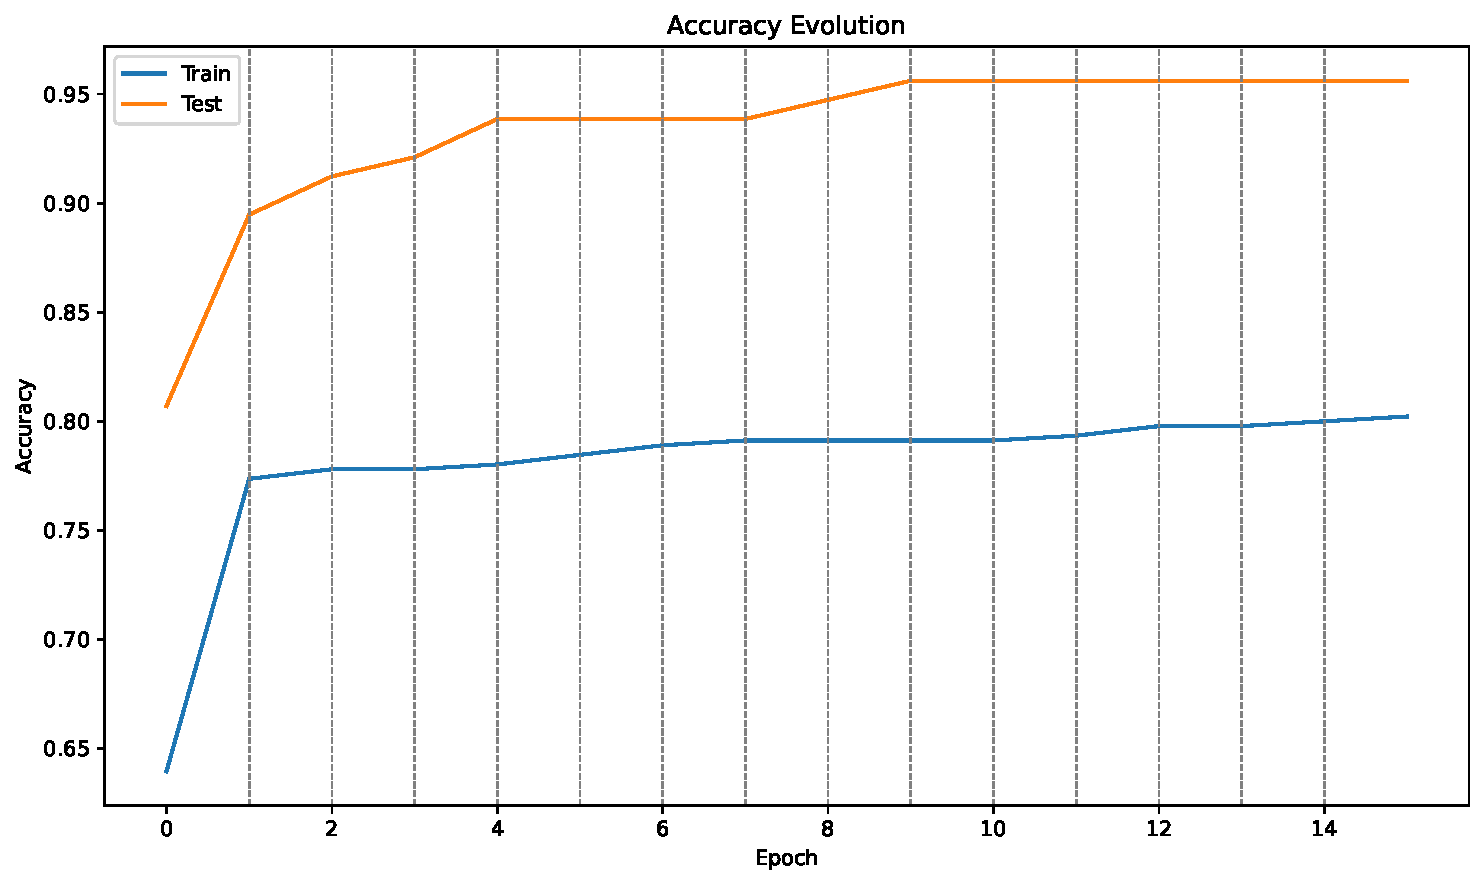
\includegraphics[width=0.3\textwidth]{latex/NN_Train_cancer_16_0.25_0.0_0.75_0.25_0.0_0.75_PathSize_None__accuracy_evolution.pdf}%
}
\subfloat[{cancer\_16\_0.25,0.25,0.5\_0.25,0.25,0.5}]{%
  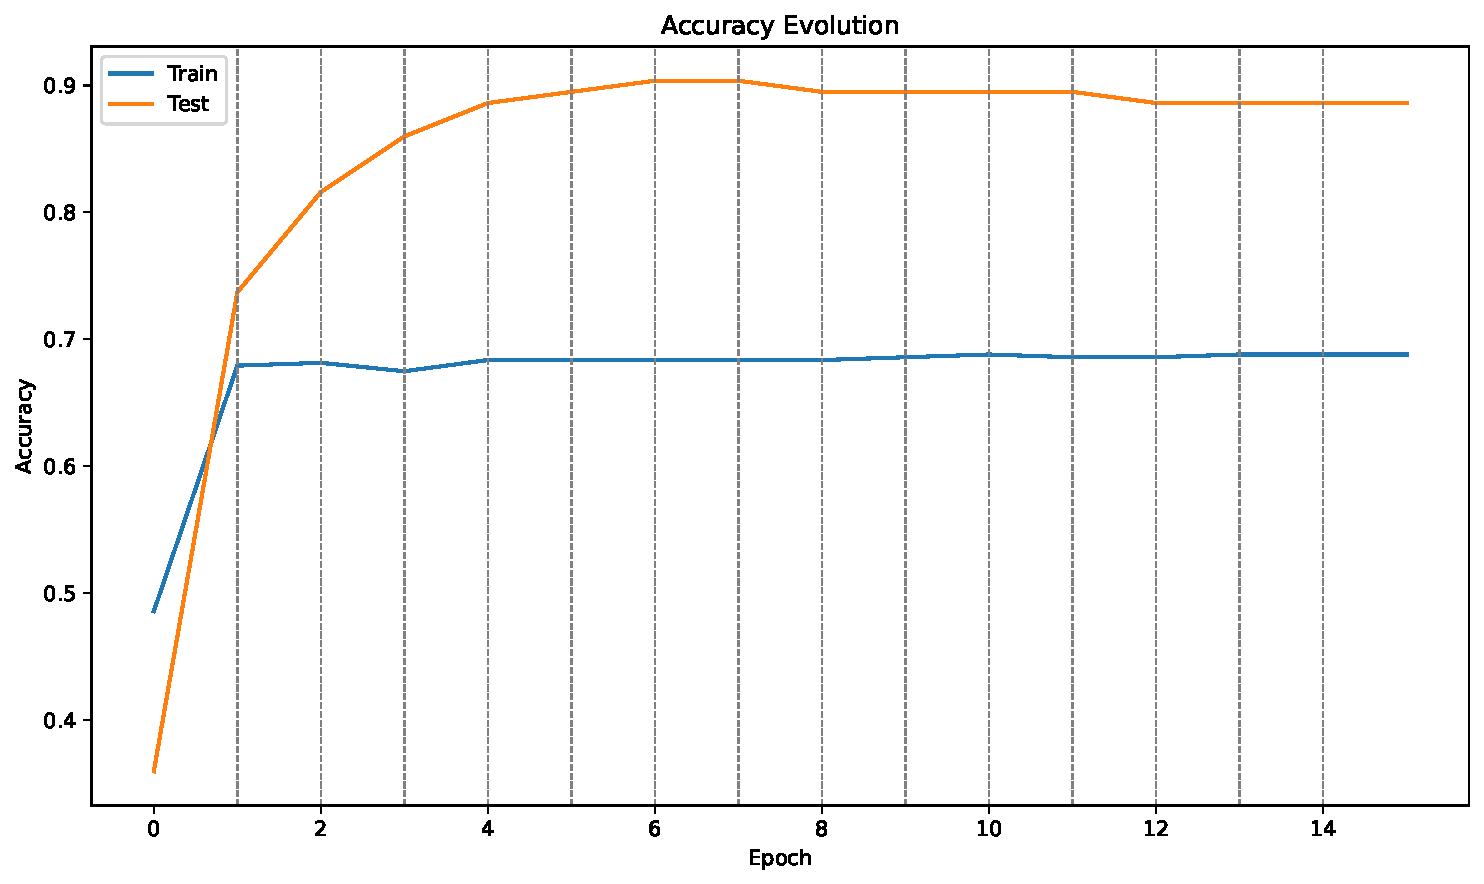
\includegraphics[width=0.3\textwidth]{latex/NN_Train_cancer_16_0.25_0.25_0.5_0.25_0.25_0.5_PathSize_None__accuracy_evolution.pdf}%
}
\subfloat[{cancer\_16\_distrust\_distrust}]{%
  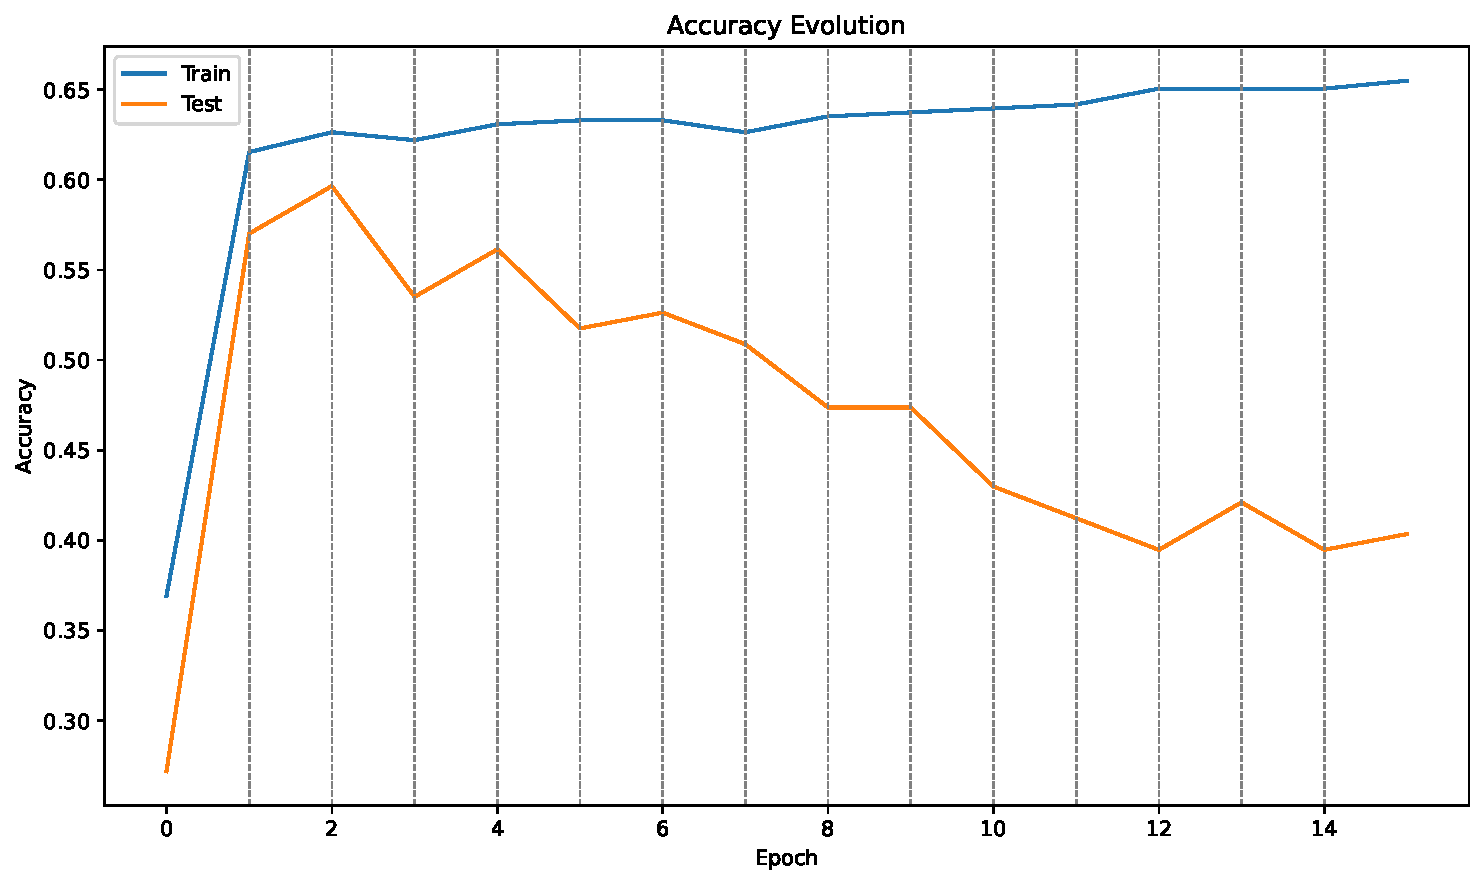
\includegraphics[width=0.3\textwidth]{latex/NN_Train_cancer_16_distrust_distrust_PathSize_None__accuracy_evolution.pdf}%
}
\\
\subfloat[{cancer\_16\_distrust\_trust}]{%
  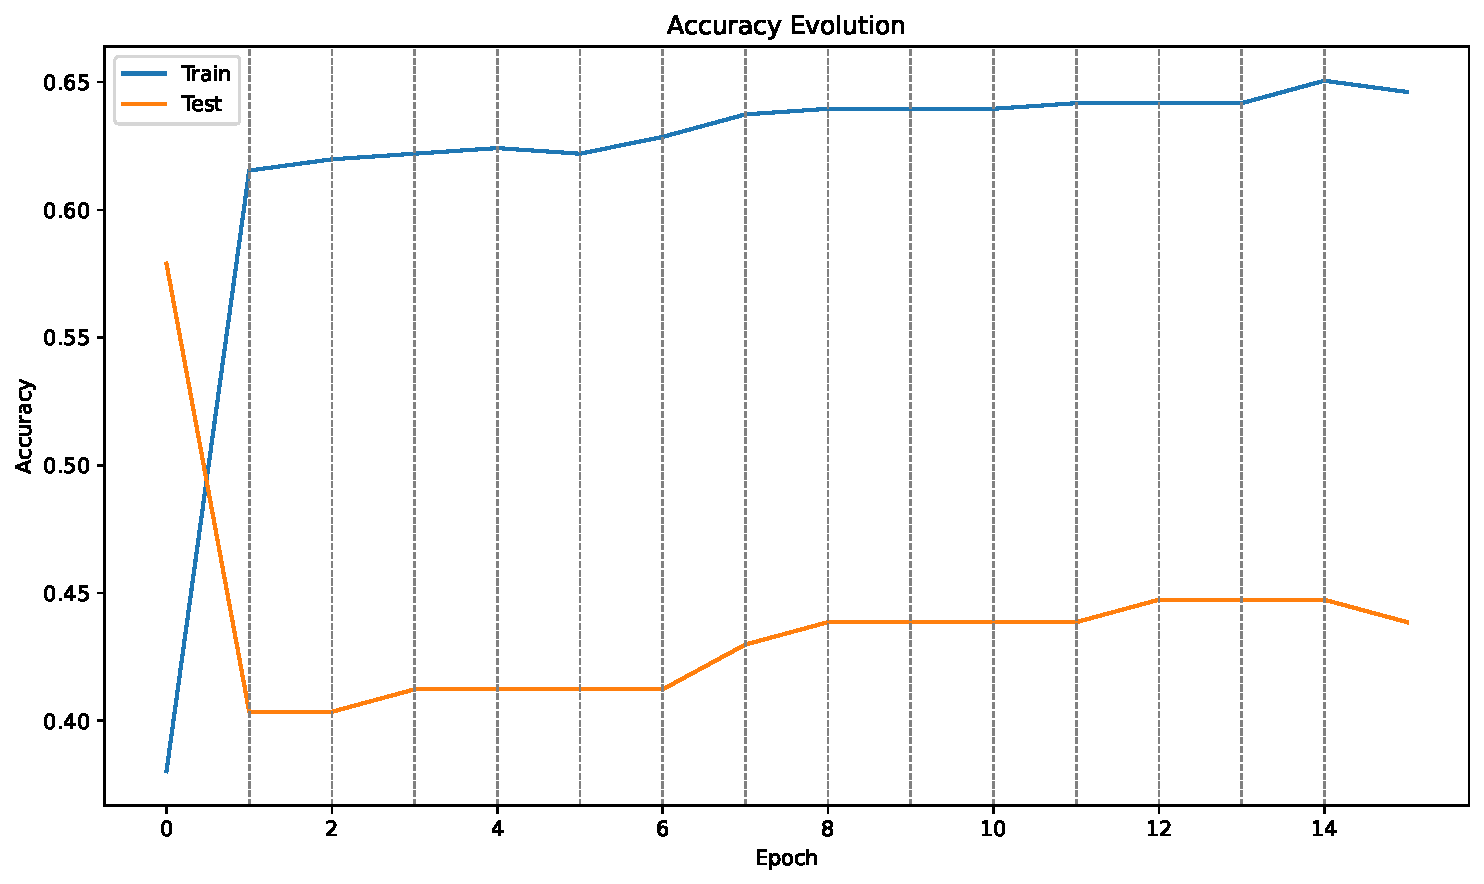
\includegraphics[width=0.3\textwidth]{latex/NN_Train_cancer_16_distrust_trust_PathSize_None__accuracy_evolution.pdf}%
}
\subfloat[{cancer\_16\_distrust\_vacuous}]{%
  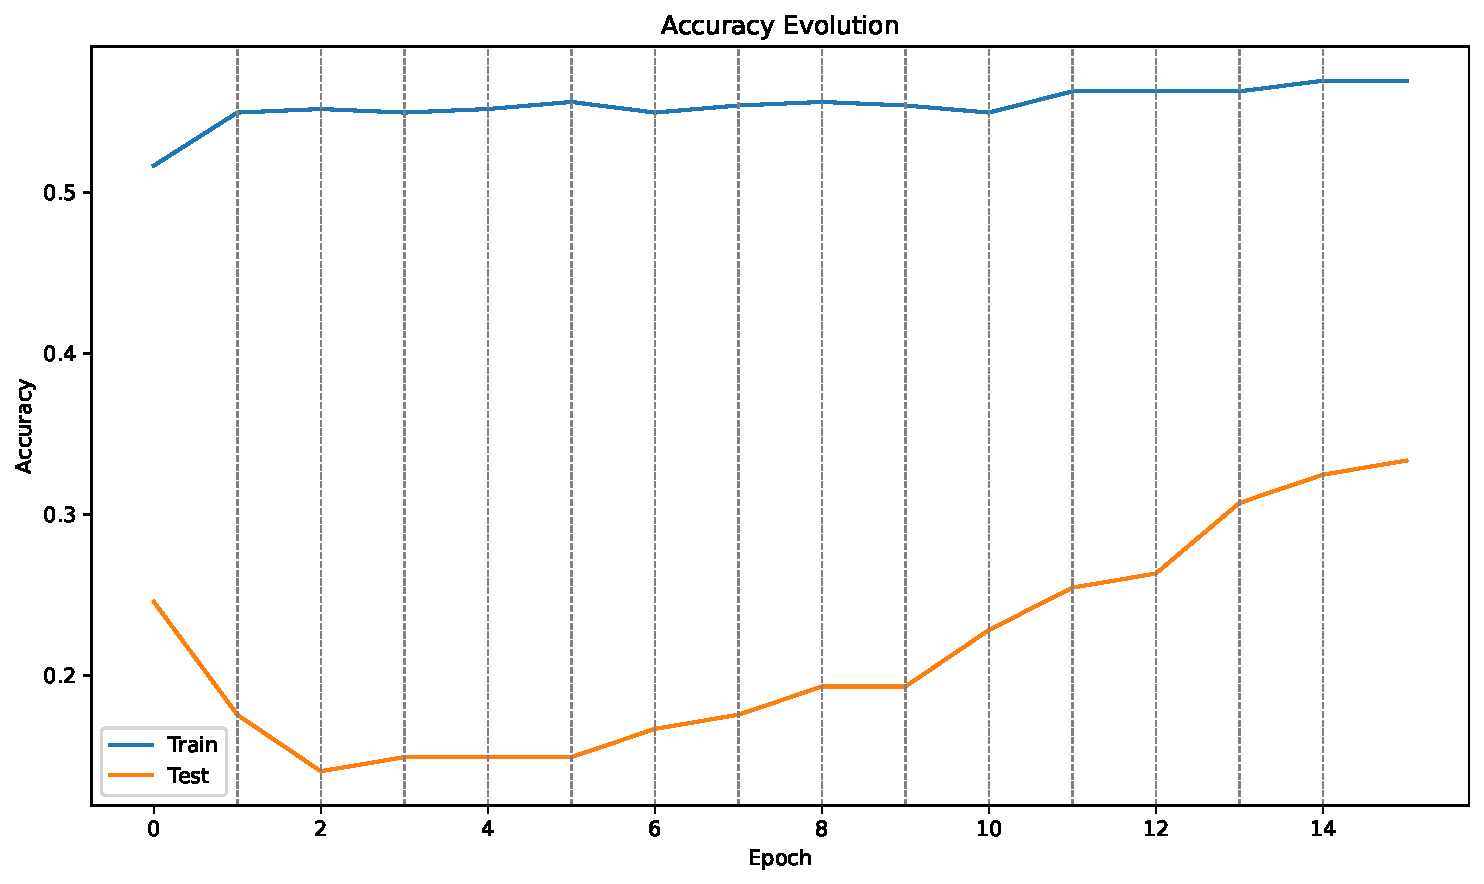
\includegraphics[width=0.3\textwidth]{latex/NN_Train_cancer_16_distrust_vacuous_PathSize_None__accuracy_evolution.pdf}%
}
\subfloat[{cancer\_16\_trust\_distrust}]{%
  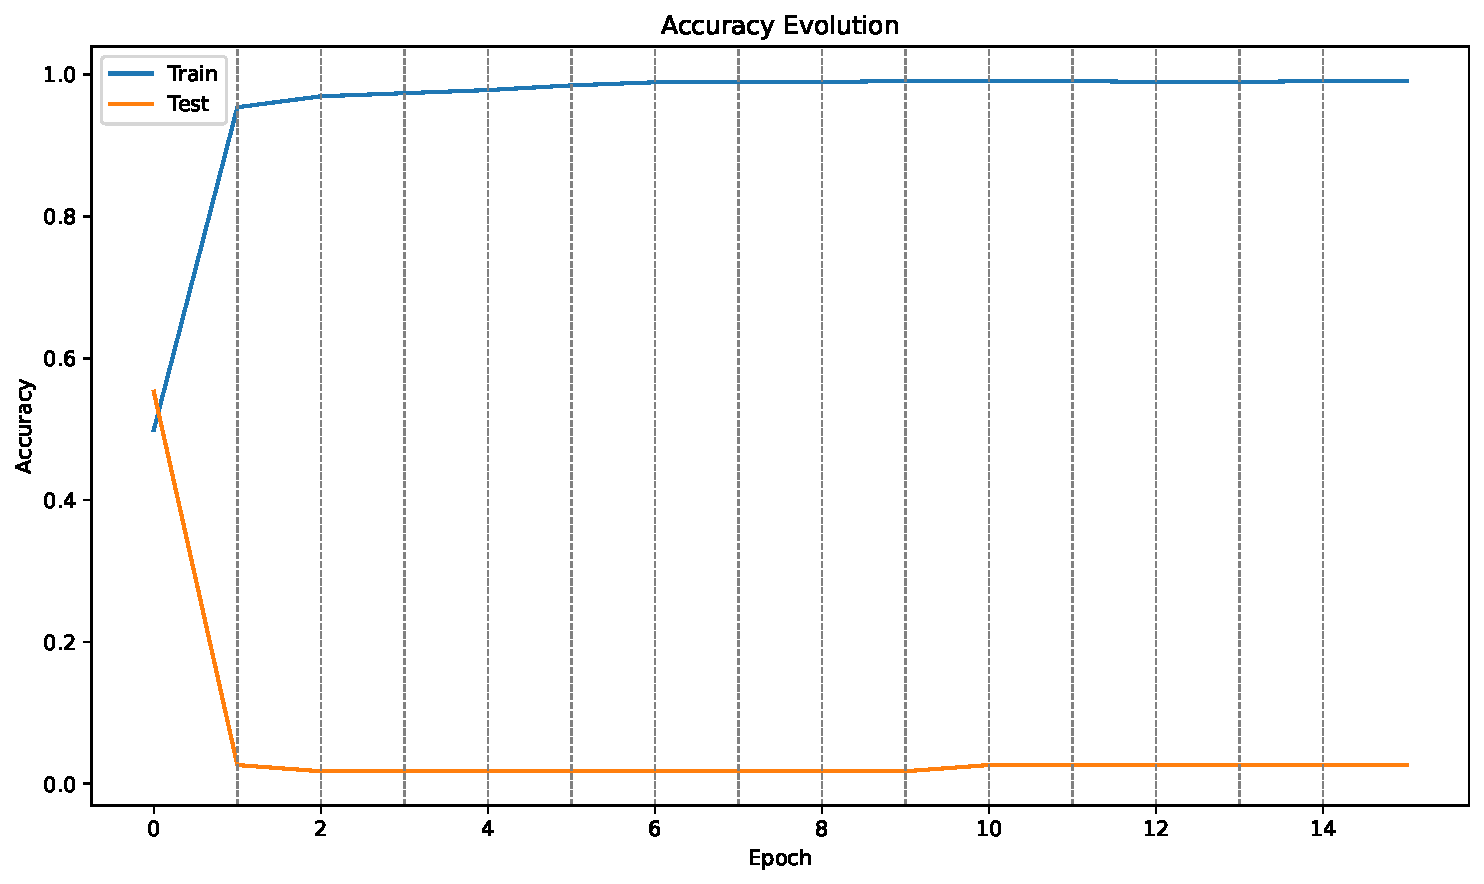
\includegraphics[width=0.3\textwidth]{latex/NN_Train_cancer_16_trust_distrust_PathSize_None__accuracy_evolution.pdf}%
}
\\
\subfloat[{cancer\_16\_trust\_trust}]{%
  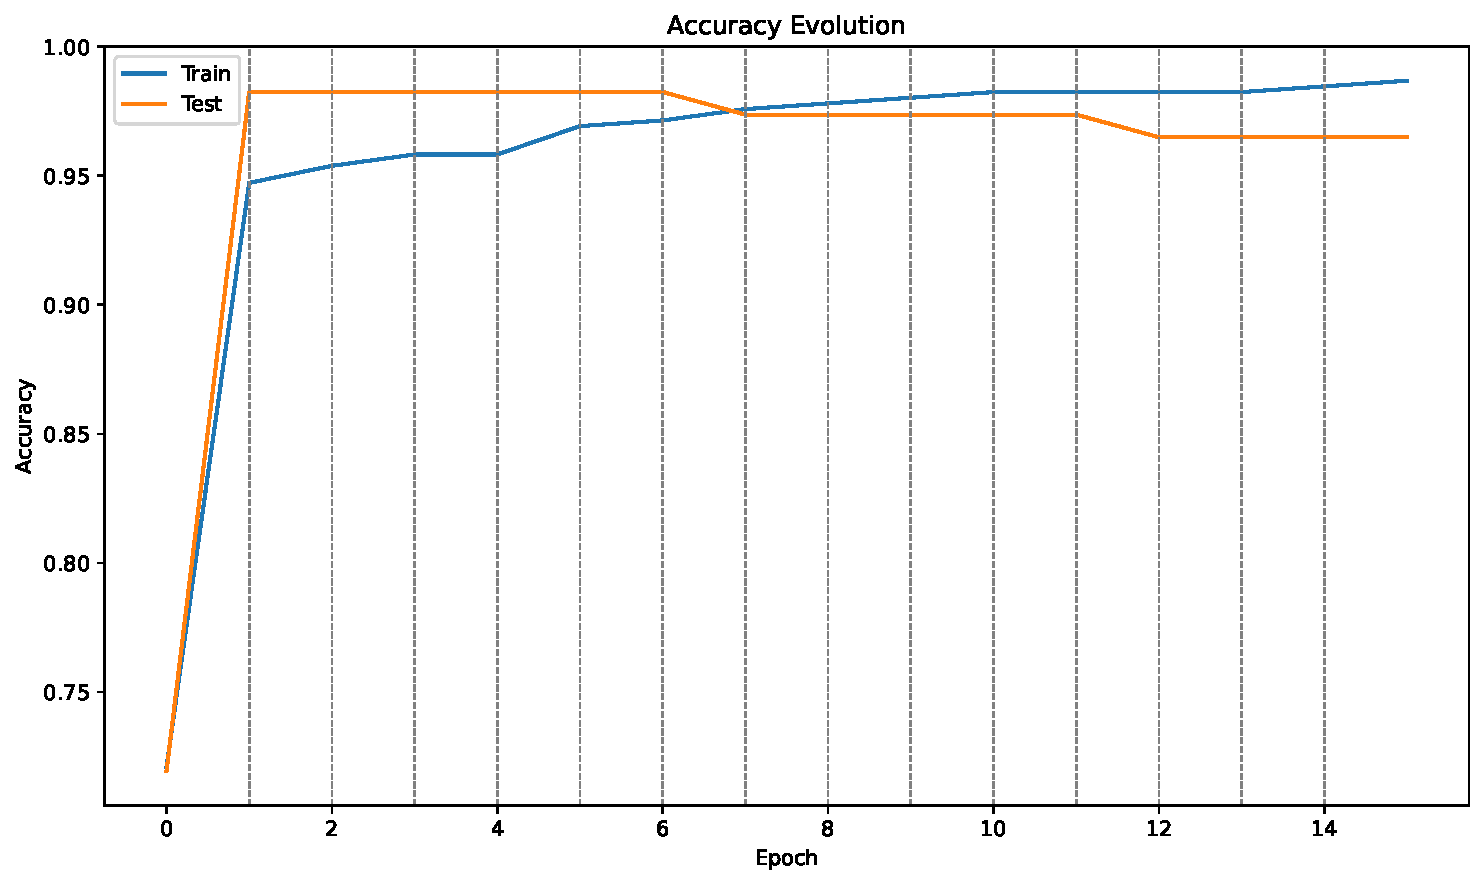
\includegraphics[width=0.3\textwidth]{latex/NN_Train_cancer_16_trust_trust_PathSize_None__accuracy_evolution.pdf}%
}
\subfloat[{cancer\_16\_trust\_vacuous}]{%
  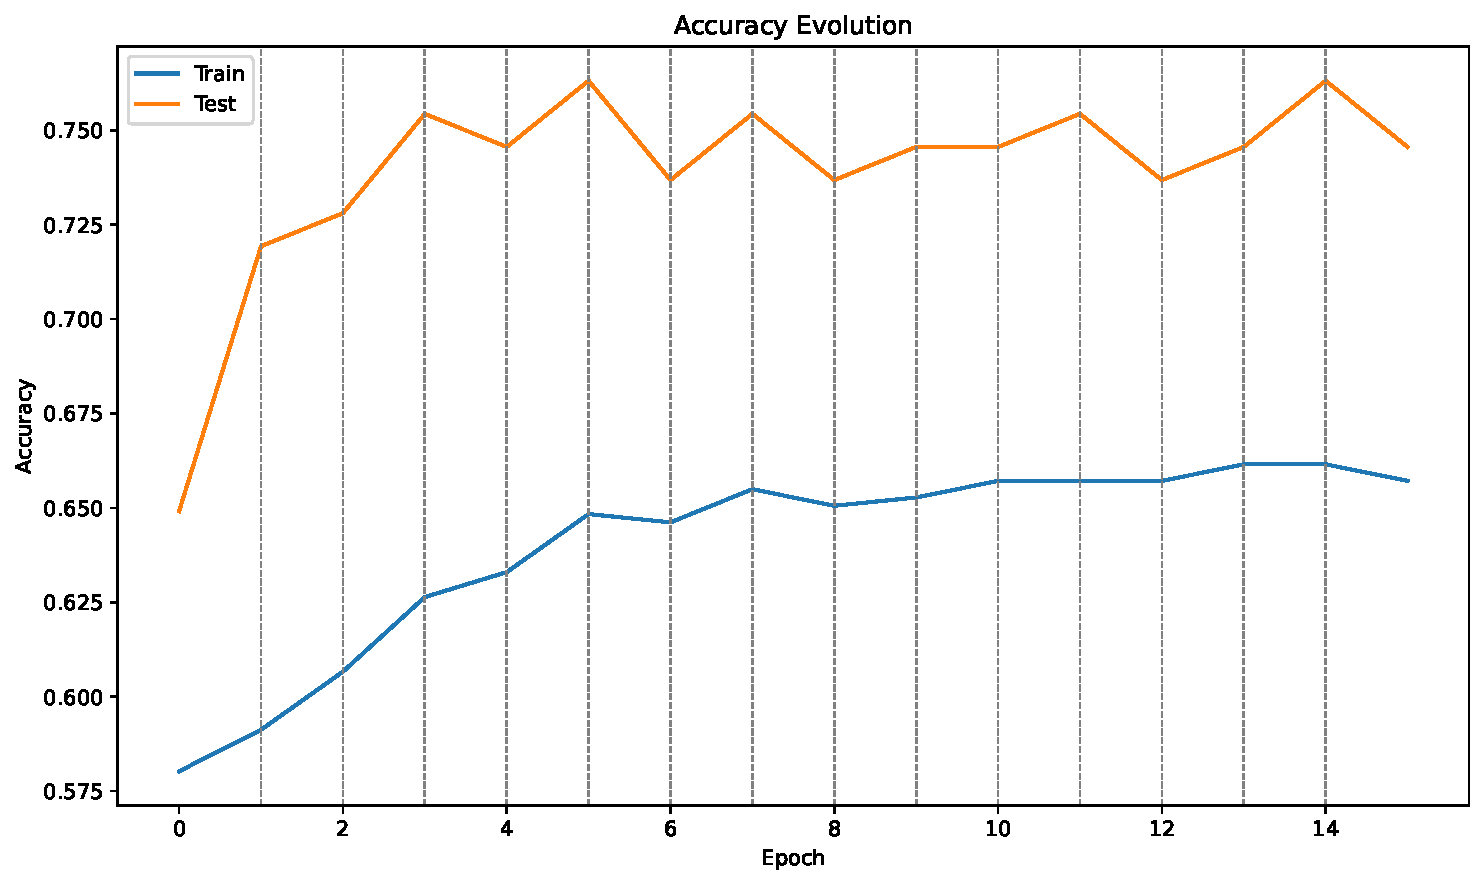
\includegraphics[width=0.3\textwidth]{latex/NN_Train_cancer_16_trust_vacuous_PathSize_None__accuracy_evolution.pdf}%
}
\subfloat[{cancer\_16\_vacuous\_distrust}]{%
  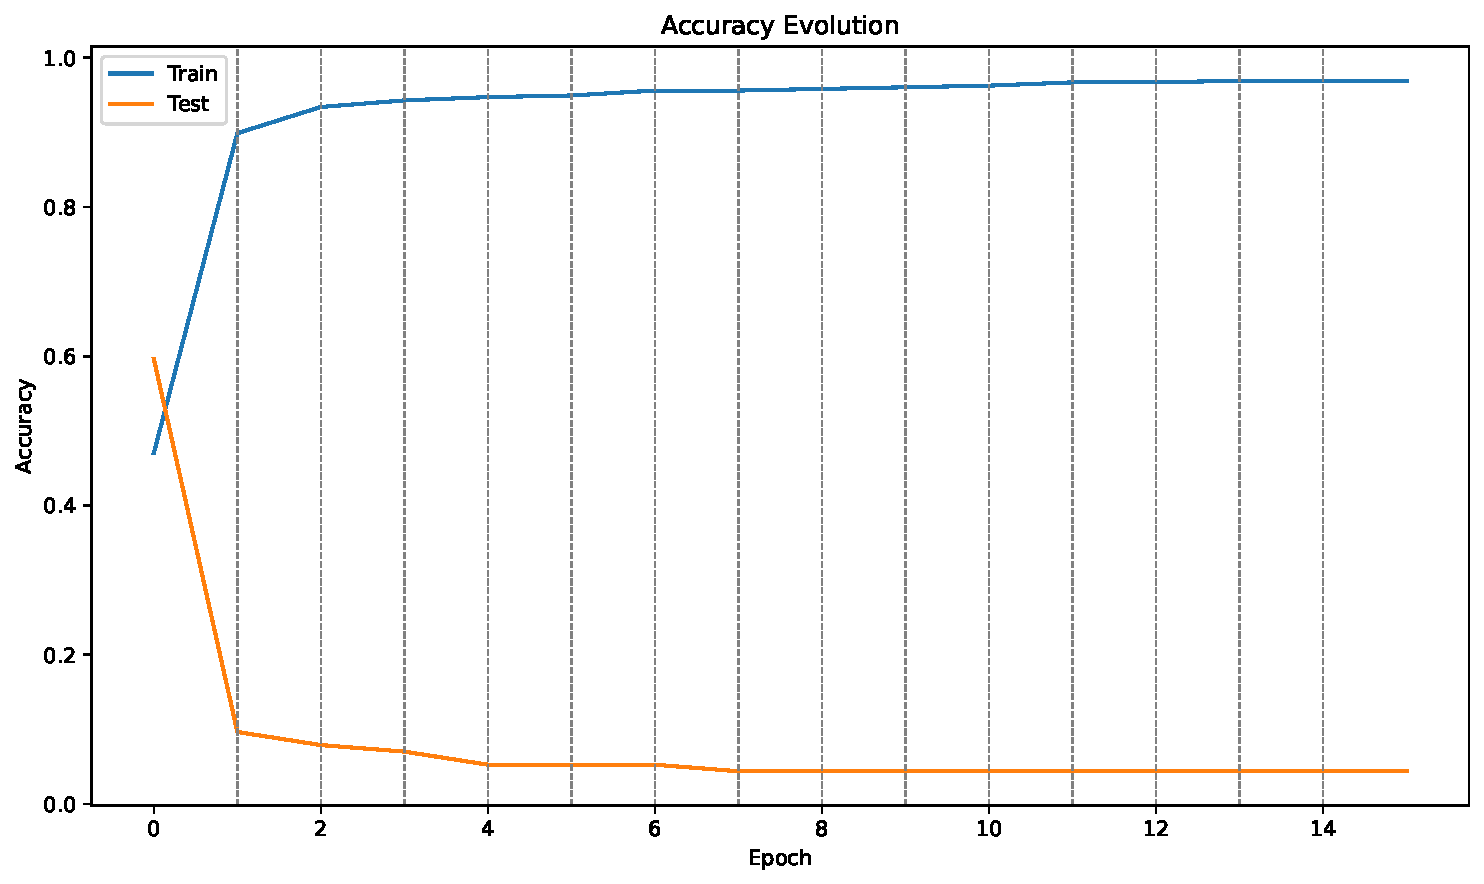
\includegraphics[width=0.3\textwidth]{latex/NN_Train_cancer_16_vacuous_distrust_PathSize_None__accuracy_evolution.pdf}%
}
\endgroup
\\
\caption{Accuracy Evolution (1/3)}
\end{figure}

\begin{figure}[htbp]
\centering
\begingroup
\captionsetup[subfloat]{justification=centering,singlelinecheck=false, font=scriptsize}
\subfloat[{cancer\_16\_vacuous\_trust}]{%
  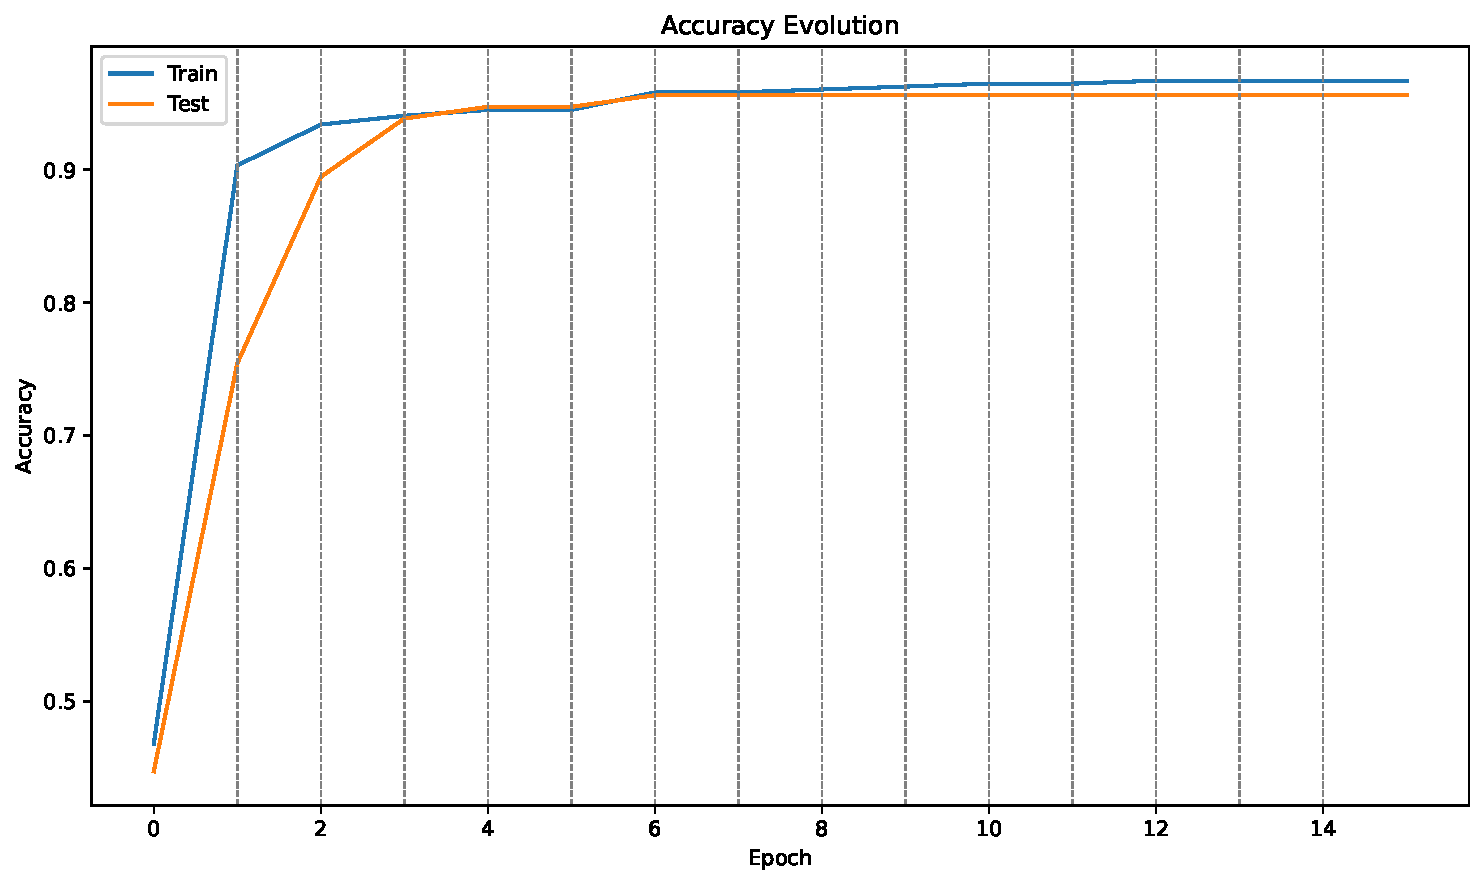
\includegraphics[width=0.3\textwidth]{latex/NN_Train_cancer_16_vacuous_trust_PathSize_None__accuracy_evolution.pdf}%
}
\subfloat[{cancer\_16\_vacuous\_vacuous}]{%
  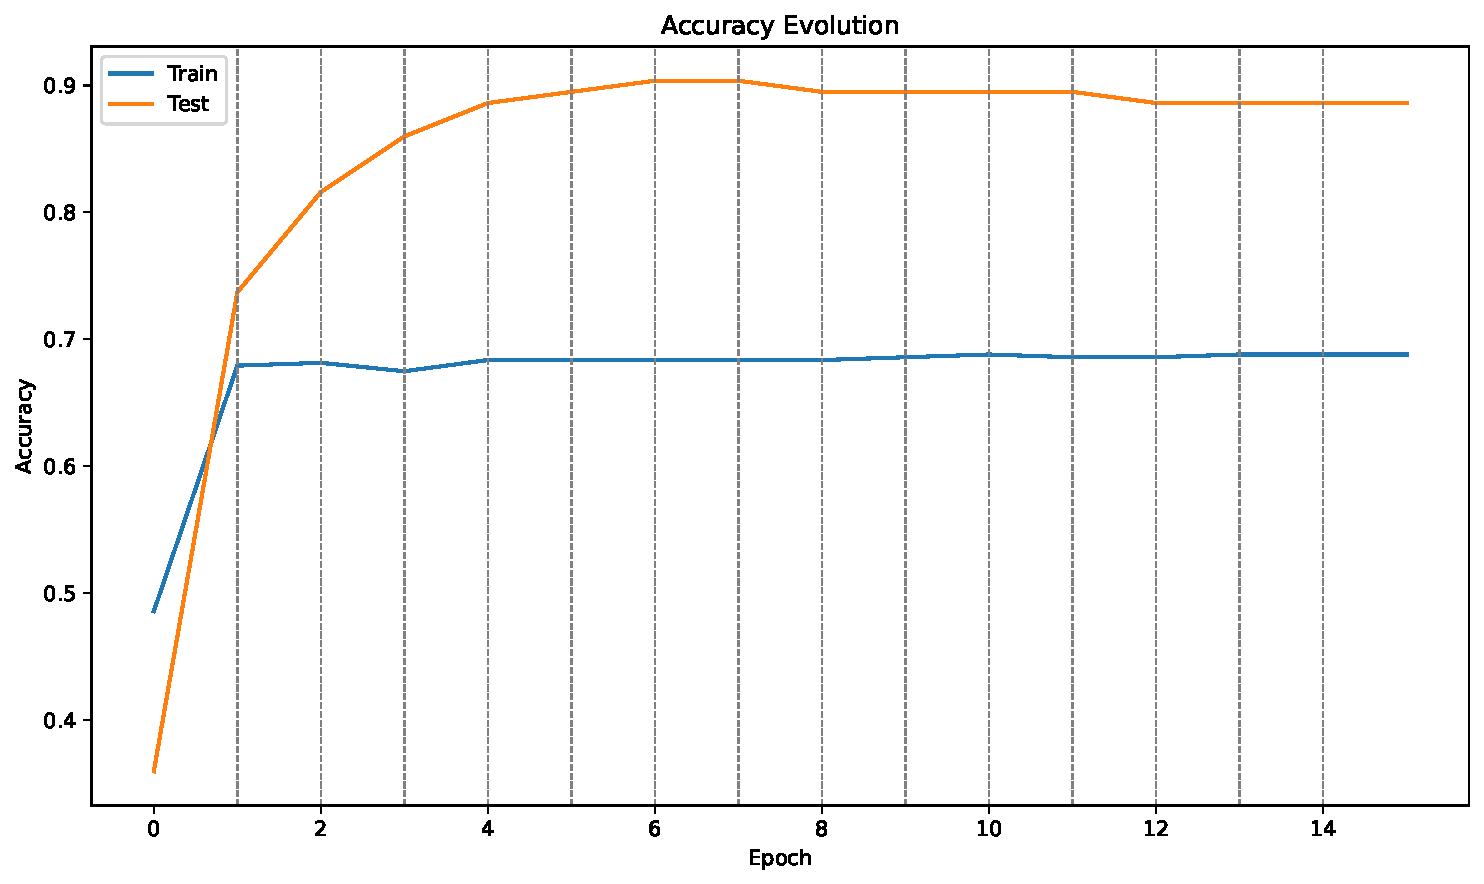
\includegraphics[width=0.3\textwidth]{latex/NN_Train_cancer_16_vacuous_vacuous_PathSize_None__accuracy_evolution.pdf}%
}
\subfloat[{mnist\_128\_trust\_trust, ps=1}]{%
  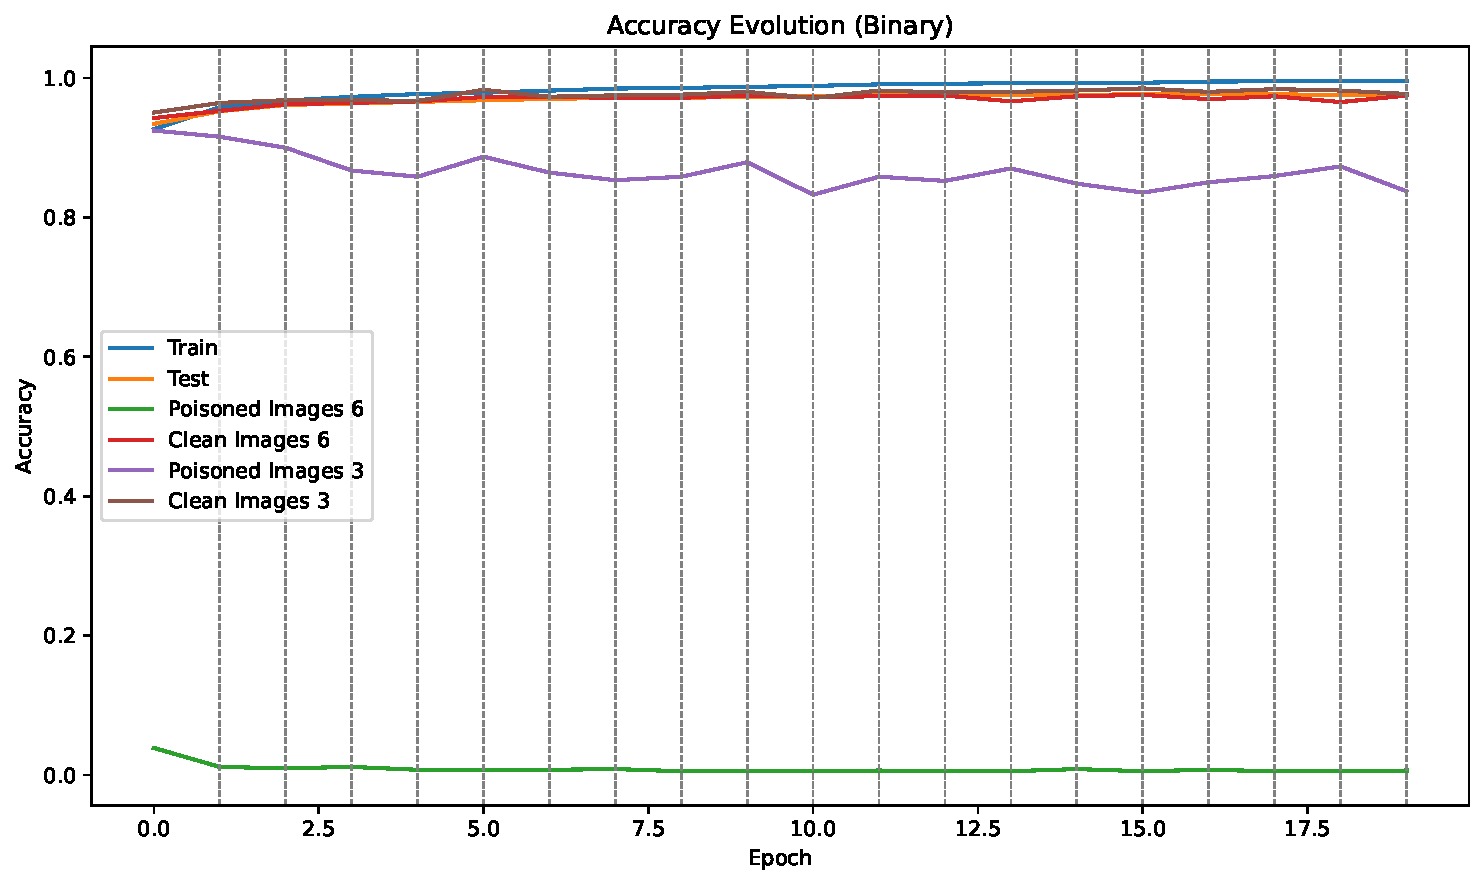
\includegraphics[width=0.3\textwidth]{latex/NN_Train_mnist_128_trust_trust_PathSize_1__accuracy_evolution.pdf}%
}
\\
\subfloat[{mnist\_128\_trust\_trust, ps=10}]{%
  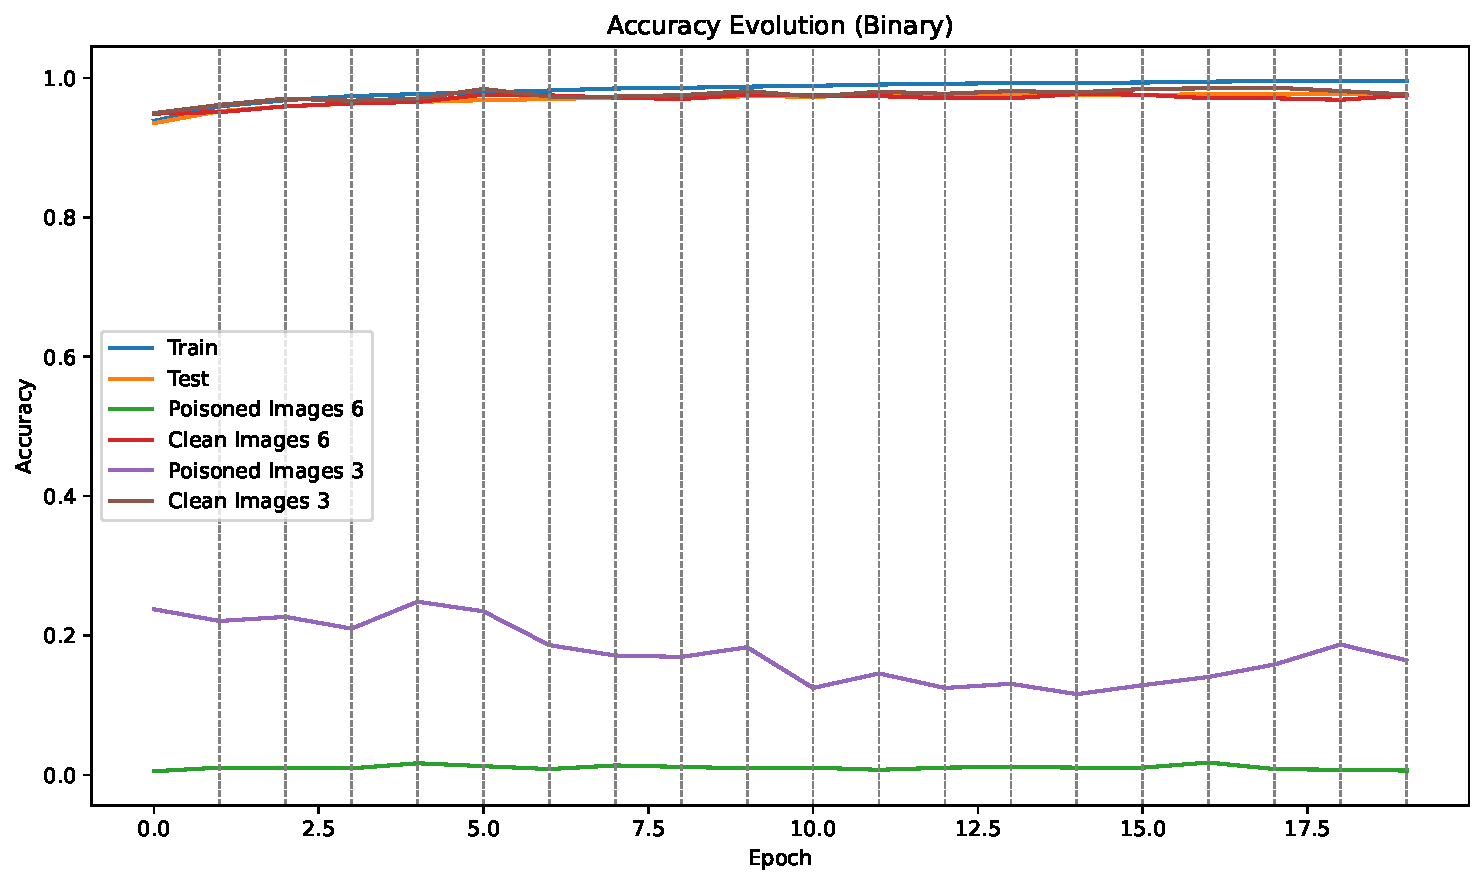
\includegraphics[width=0.3\textwidth]{latex/NN_Train_mnist_128_trust_trust_PathSize_10__accuracy_evolution.pdf}%
}
\subfloat[{mnist\_128\_trust\_trust, ps=27}]{%
  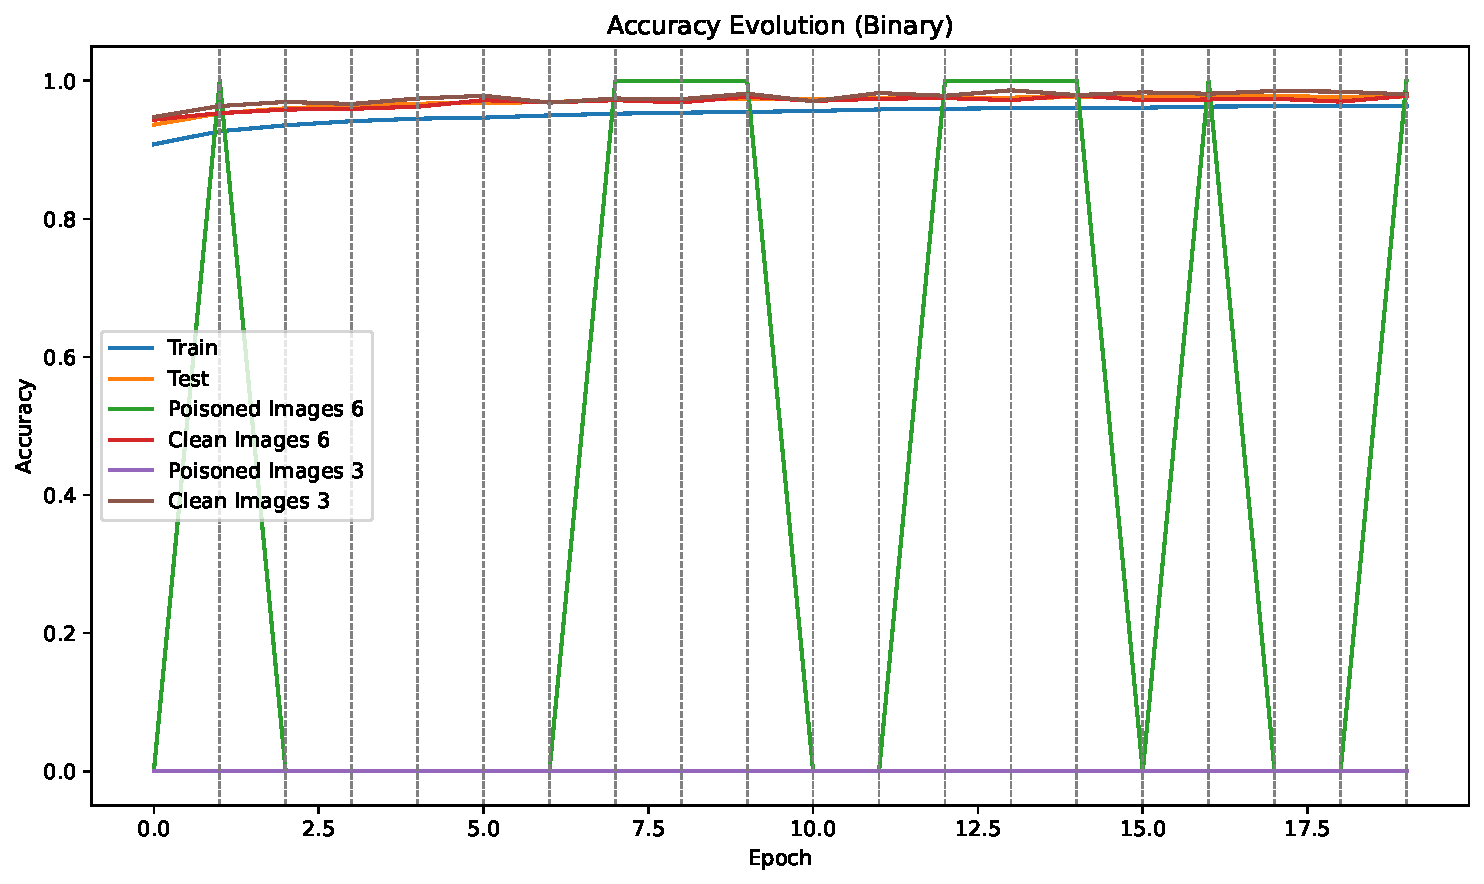
\includegraphics[width=0.3\textwidth]{latex/NN_Train_mnist_128_trust_trust_PathSize_27__accuracy_evolution.pdf}%
}
\subfloat[{mnist\_128\_trust\_trust, ps=4}]{%
  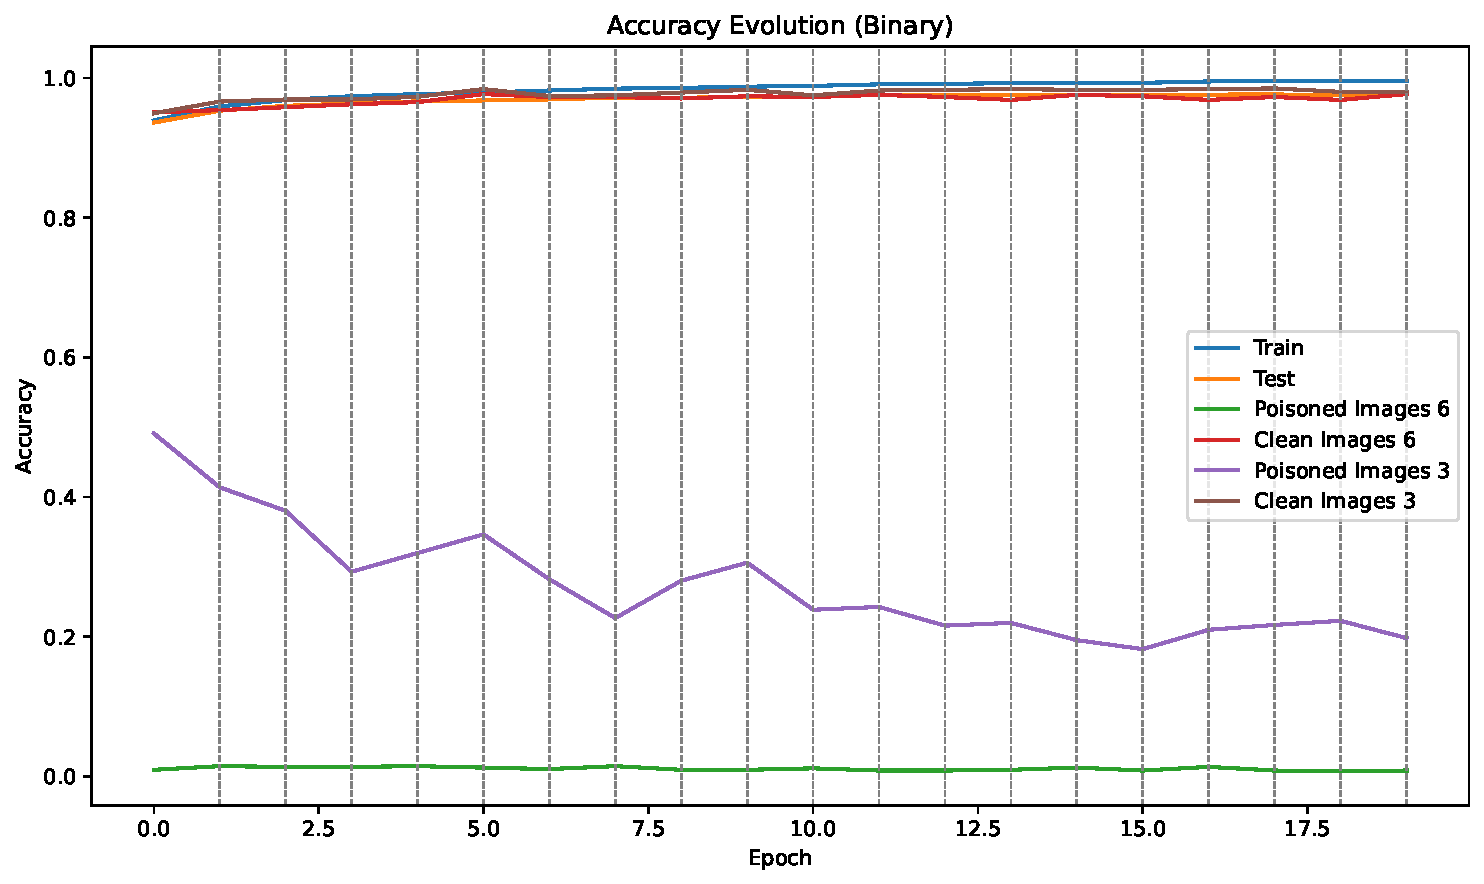
\includegraphics[width=0.3\textwidth]{latex/NN_Train_mnist_128_trust_trust_PathSize_4__accuracy_evolution.pdf}%
}
\\
\subfloat[{mnist\_128\_vacuous\_vacuous}]{%
  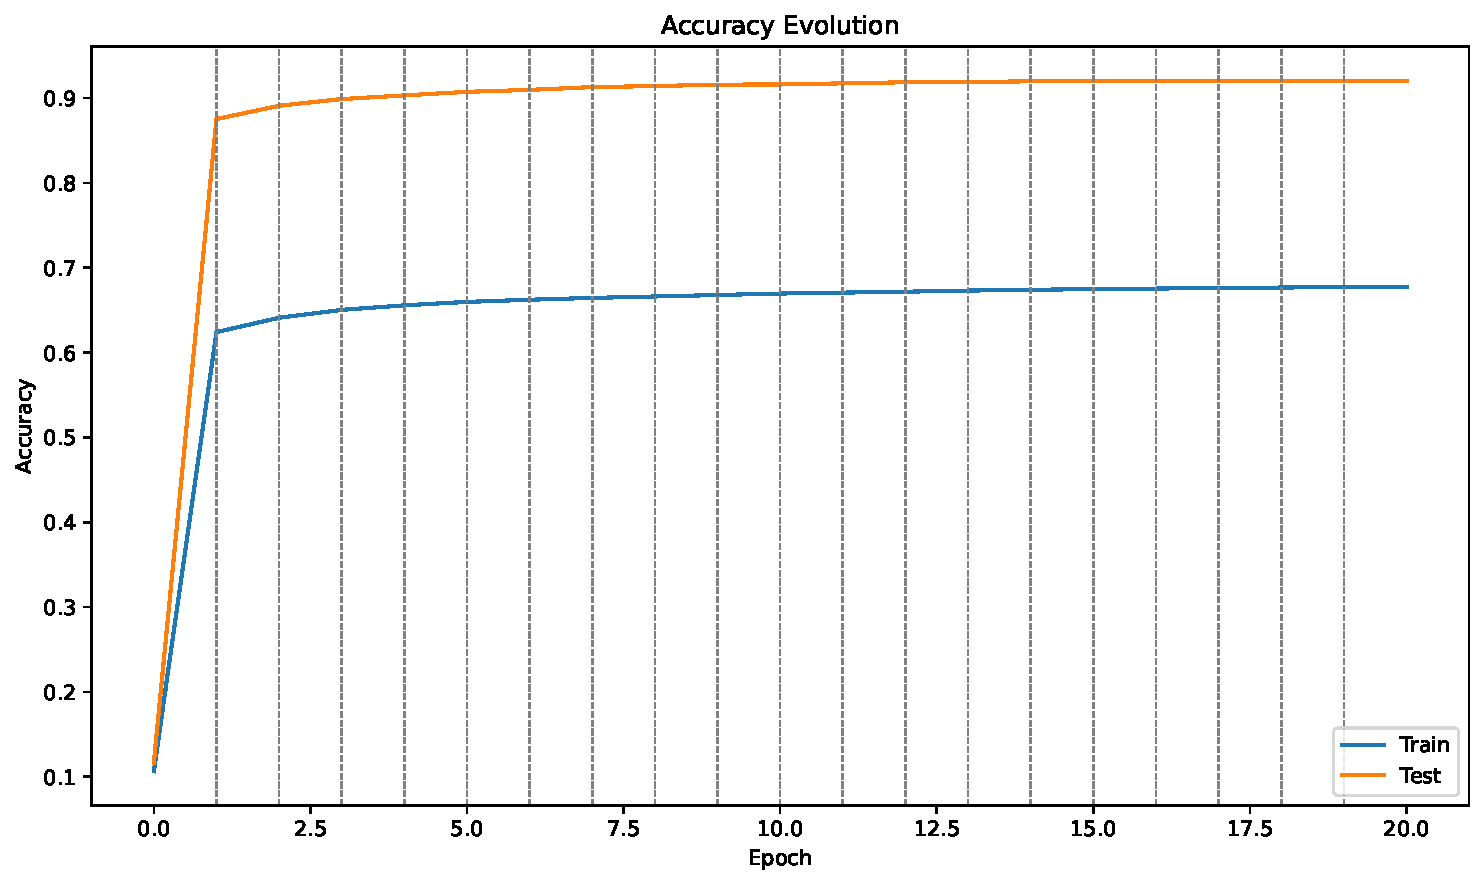
\includegraphics[width=0.3\textwidth]{latex/NN_Train_mnist_128_vacuous_vacuous_PathSize_None__accuracy_evolution.pdf}%
}
\subfloat[{mnist\_16\_16\_trust\_trust}]{%
  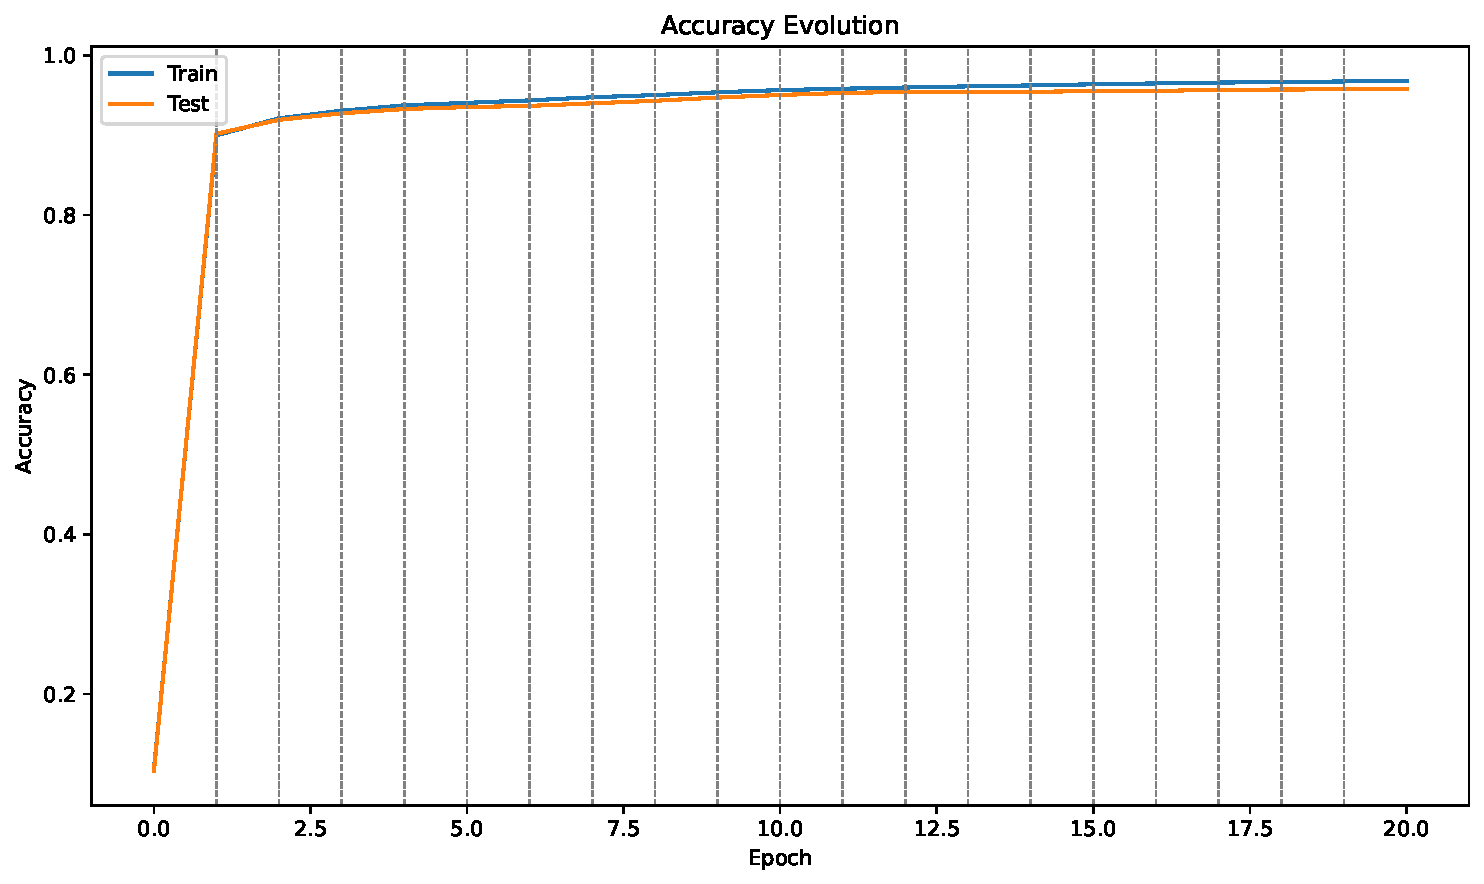
\includegraphics[width=0.3\textwidth]{latex/NN_Train_mnist_16_16_trust_trust_PathSize_None__accuracy_evolution.pdf}%
}
\subfloat[{mnist\_16\_16\_vacuous\_vacuous}]{%
  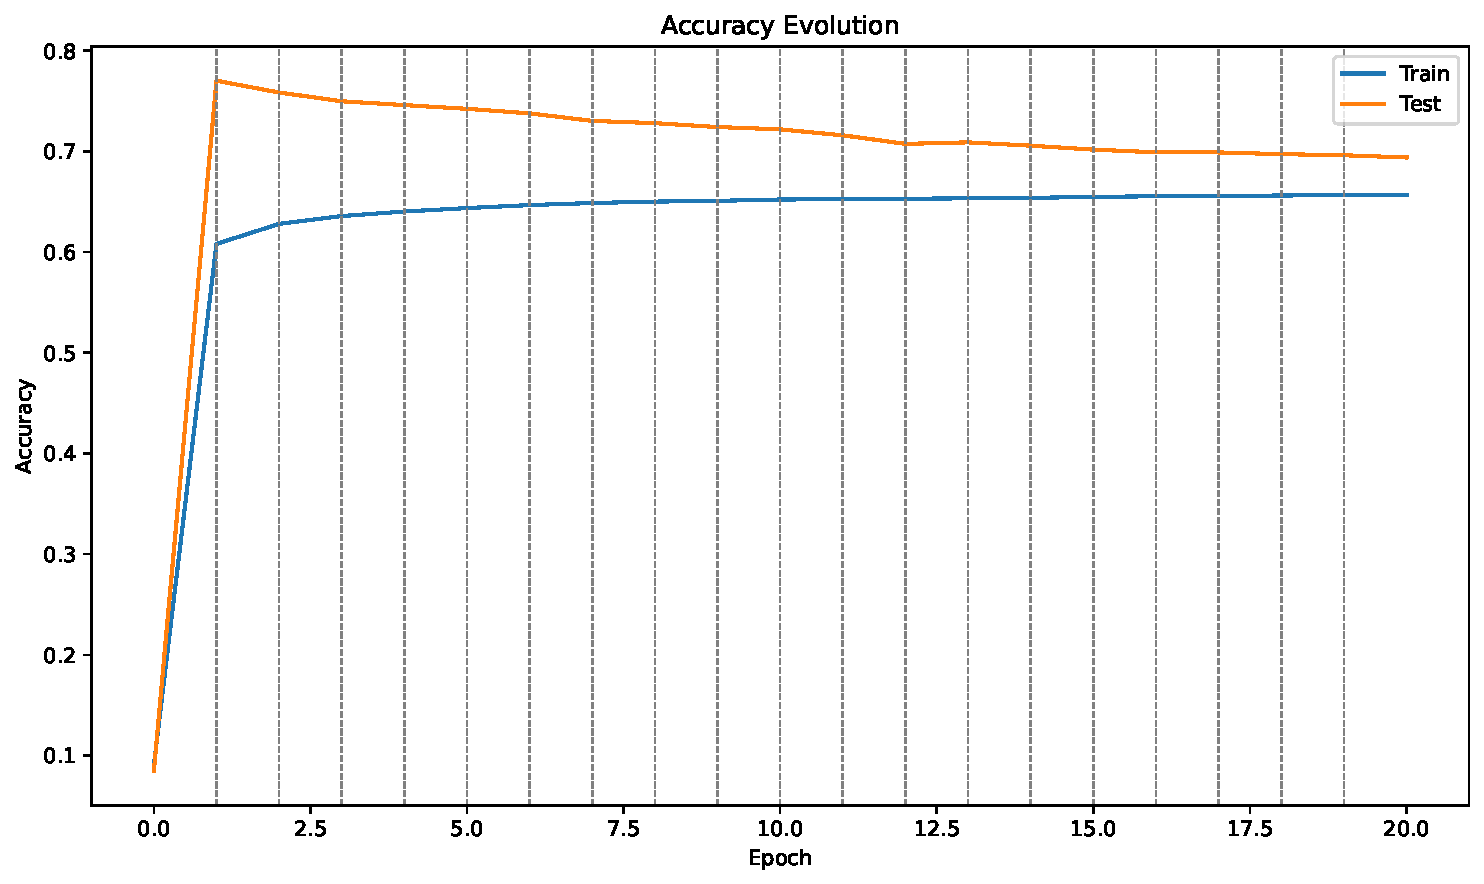
\includegraphics[width=0.3\textwidth]{latex/NN_Train_mnist_16_16_vacuous_vacuous_PathSize_None__accuracy_evolution.pdf}%
}
\endgroup
\\
\caption{Accuracy Evolution (2/3)}
\end{figure}

\begin{figure}[htbp]
\centering
\begingroup
\captionsetup[subfloat]{justification=centering,singlelinecheck=false, font=scriptsize}
\subfloat[{mnist\_16\_trust\_trust}]{%
  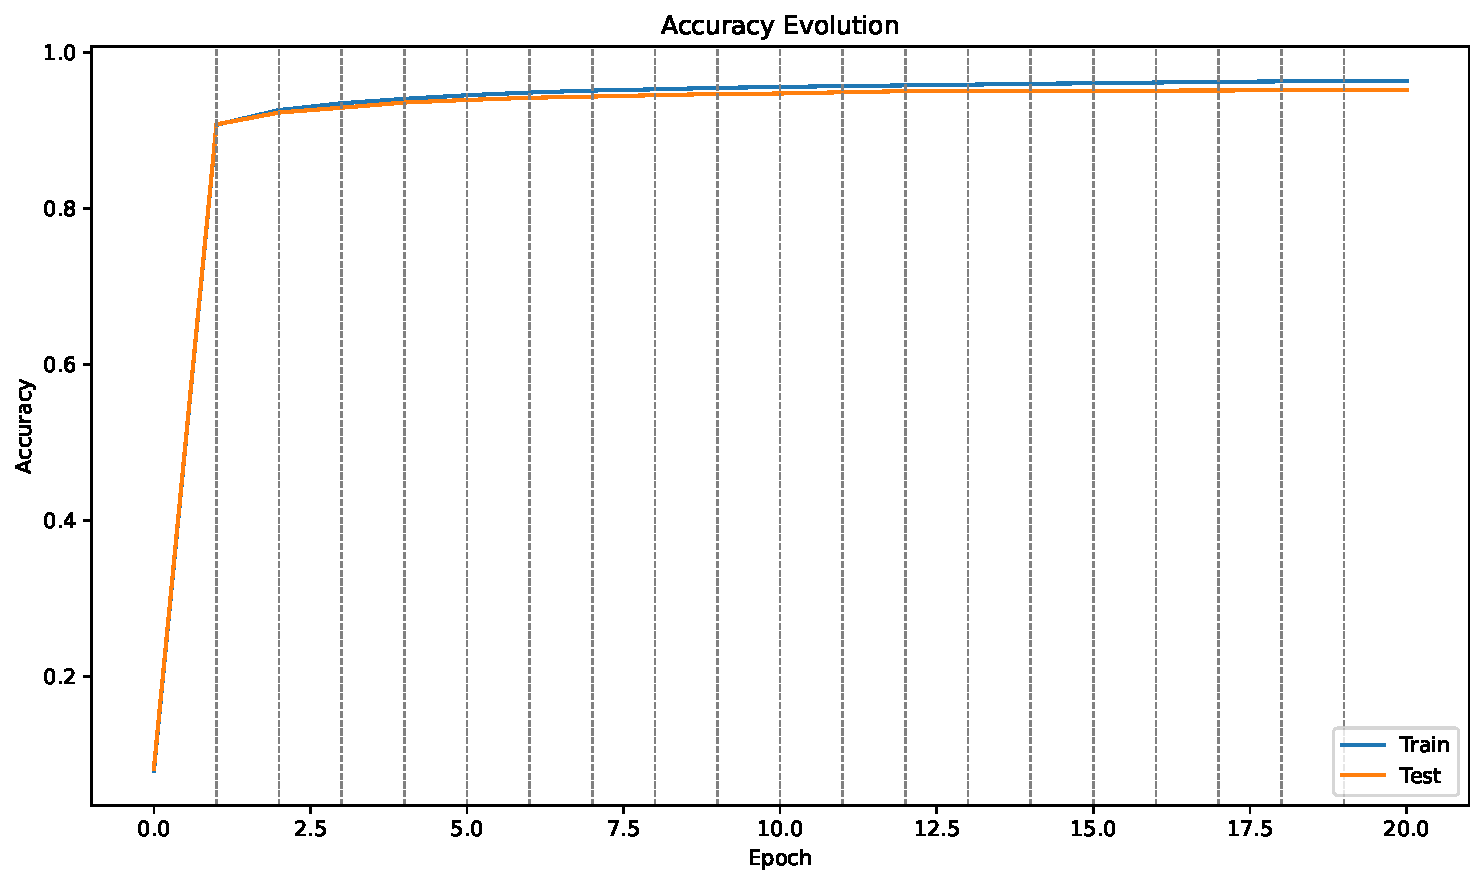
\includegraphics[width=0.3\textwidth]{latex/NN_Train_mnist_16_trust_trust_PathSize_None__accuracy_evolution.pdf}%
}
\subfloat[{mnist\_16\_vacuous\_vacuous}]{%
  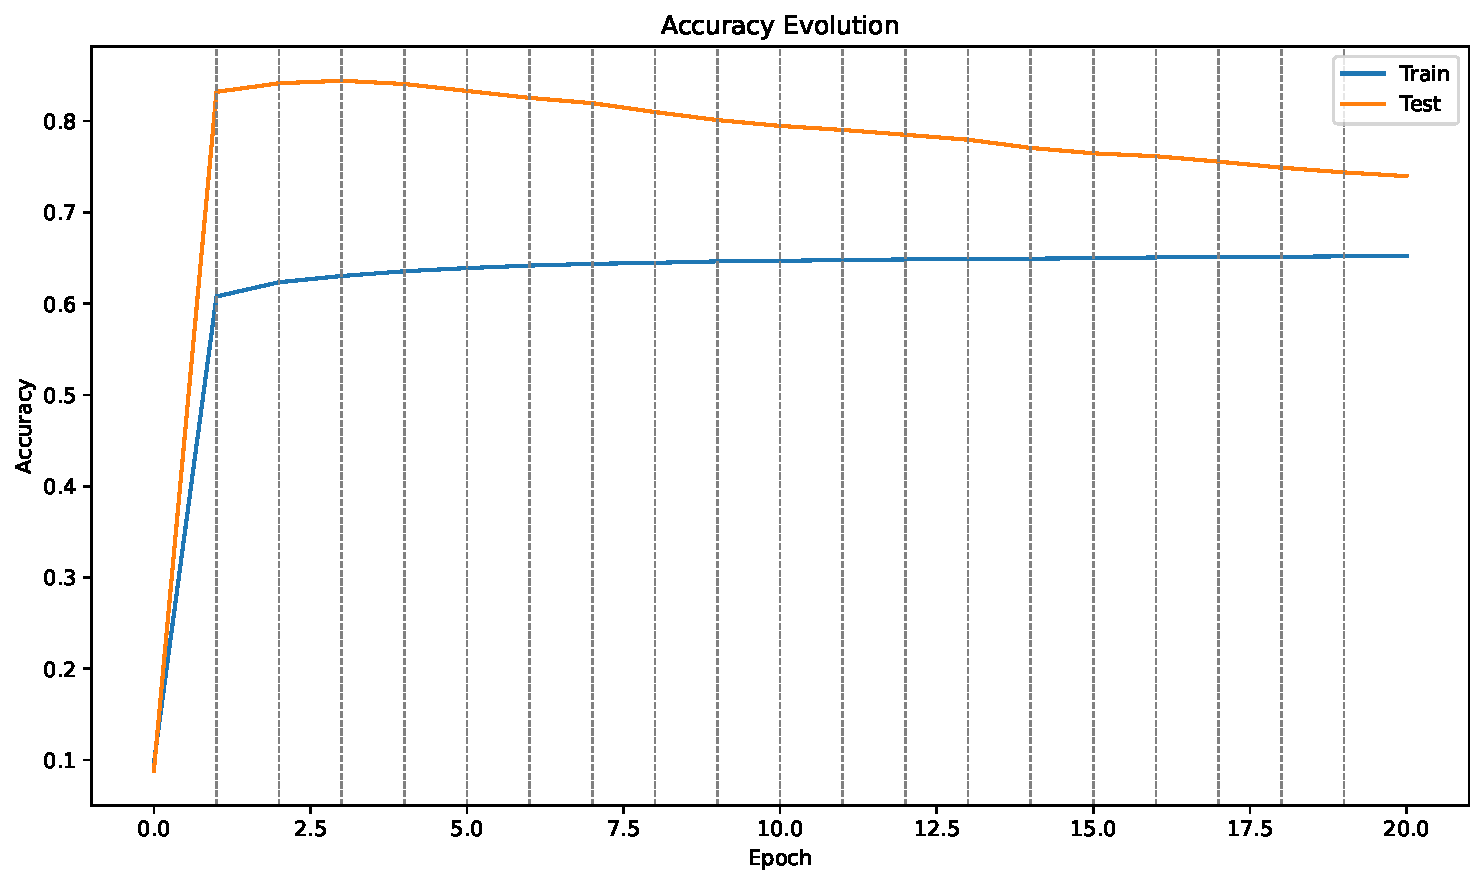
\includegraphics[width=0.3\textwidth]{latex/NN_Train_mnist_16_vacuous_vacuous_PathSize_None__accuracy_evolution.pdf}%
}
\subfloat[{mnist\_32\_vacuous\_vacuous}]{%
  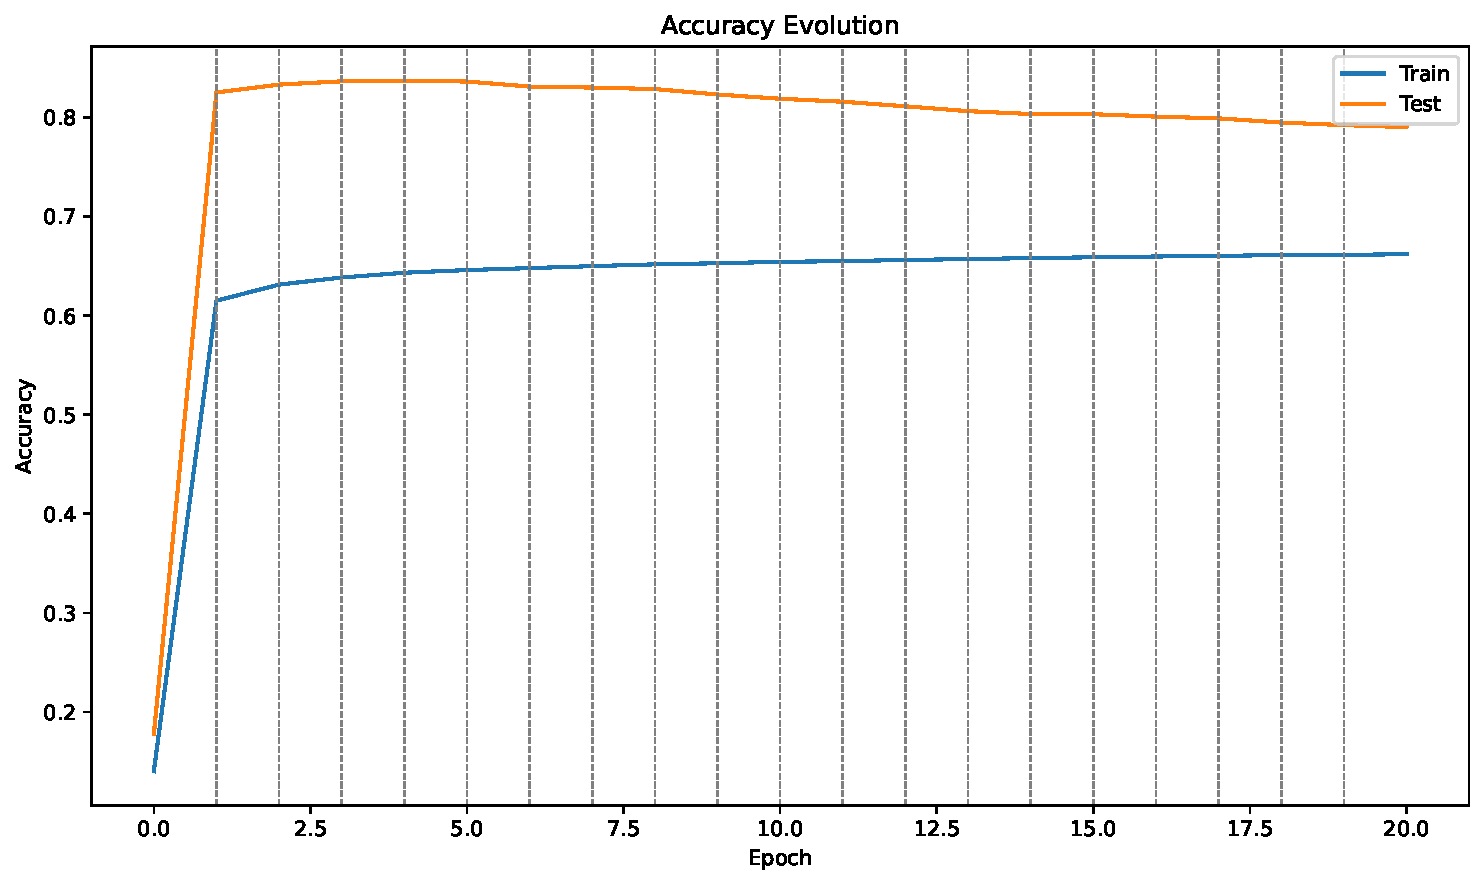
\includegraphics[width=0.3\textwidth]{latex/NN_Train_mnist_32_vacuous_vacuous_PathSize_None__accuracy_evolution.pdf}%
}
\\
\subfloat[{mnist\_64\_vacuous\_vacuous}]{%
  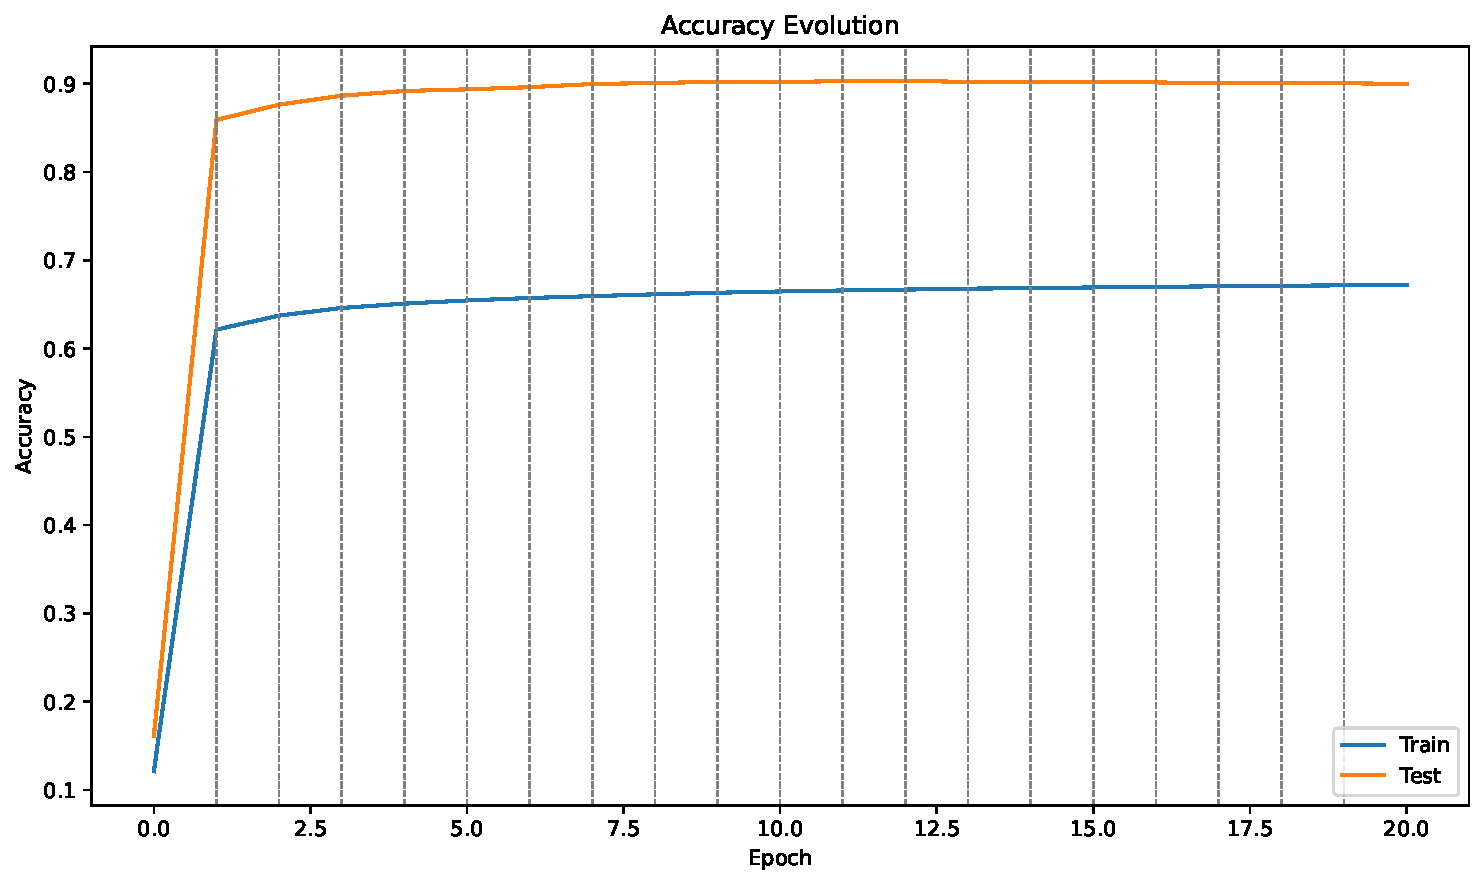
\includegraphics[width=0.3\textwidth]{latex/NN_Train_mnist_64_vacuous_vacuous_PathSize_None__accuracy_evolution.pdf}%
}
\endgroup
\caption{Accuracy Evolution (3/3)}
\end{figure}


\section{\acs{PaTAS} Evaluation Results}

\subsection{Cancer Dataset}

\subsubsection{(0.25, 0.0, 0.75) -- (0.25, 0.0, 0.75)}

\begin{figure}[htbp]
\centering
  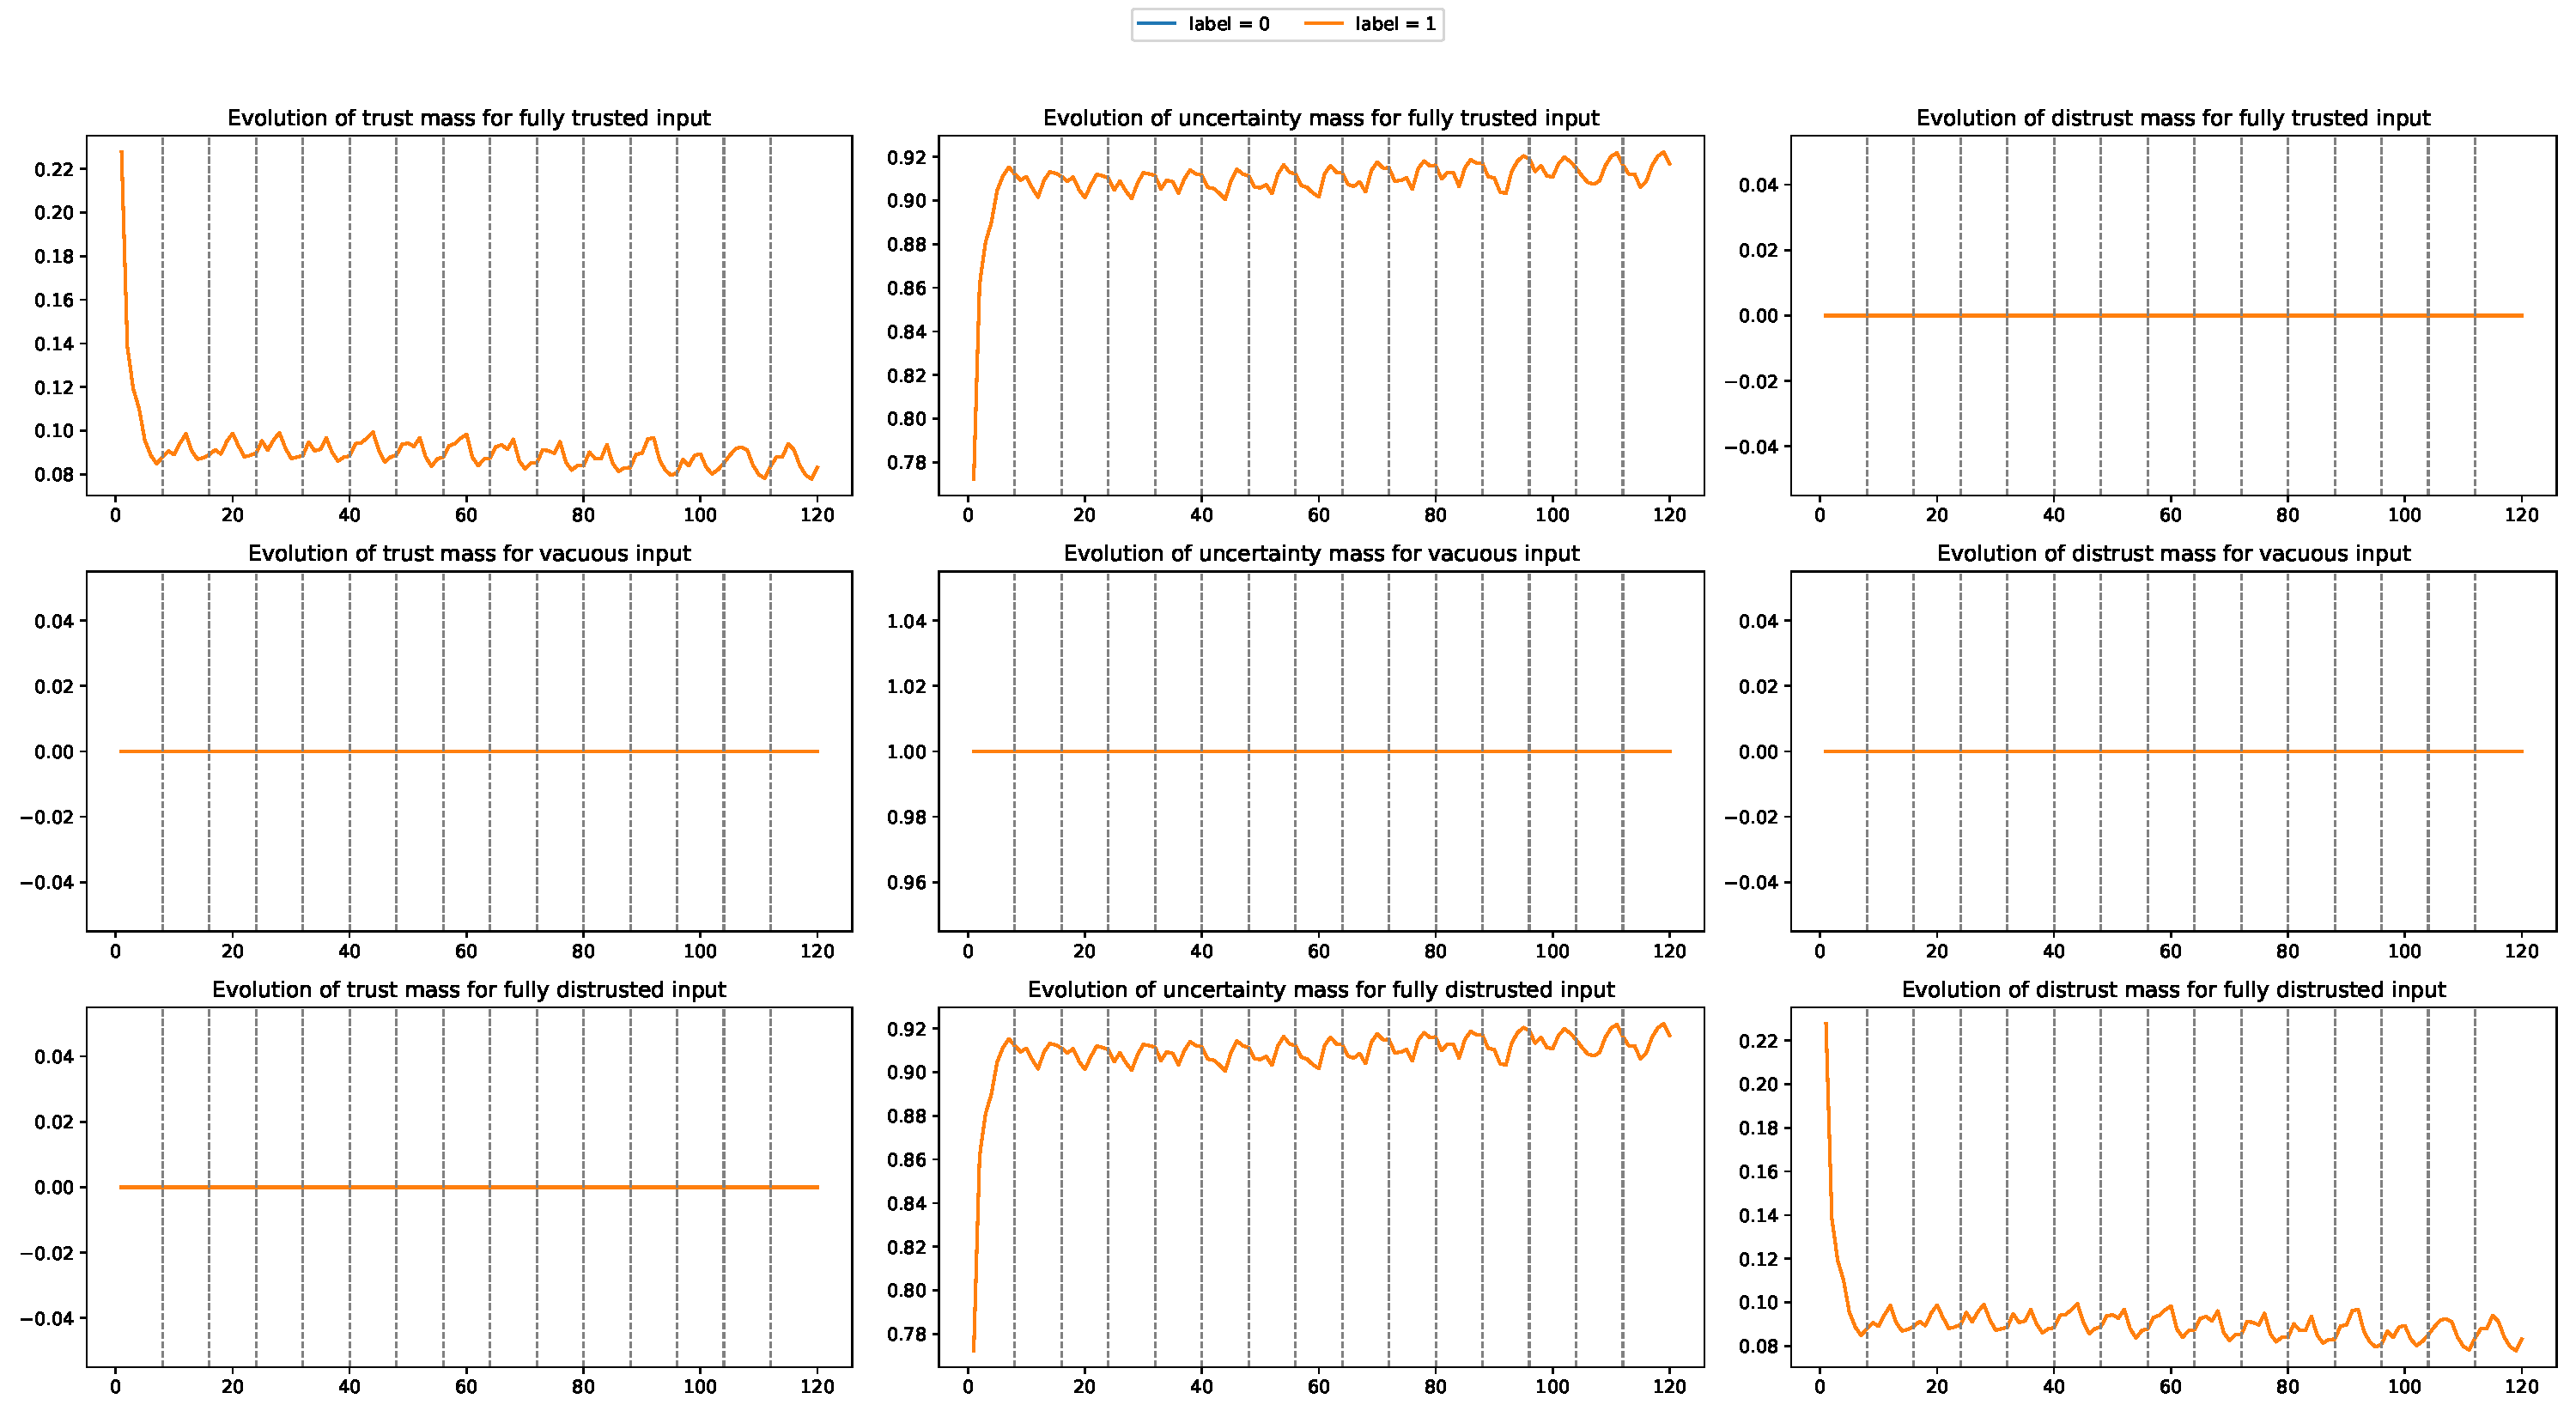
\includegraphics[width=0.8\textwidth]{latex/PTAS_Eval_cancer_16_0.25_0.0_0.75_0.25_0.0_0.75_eps_0.001_PathSize_None__plot_ptas.pdf}
\caption{cancer\_16\_0.25,0.0,0.75\_0.25,0.0,0.75, $\varepsilon$=0.001}
\end{figure}

\begin{figure}[htbp]
\centering
  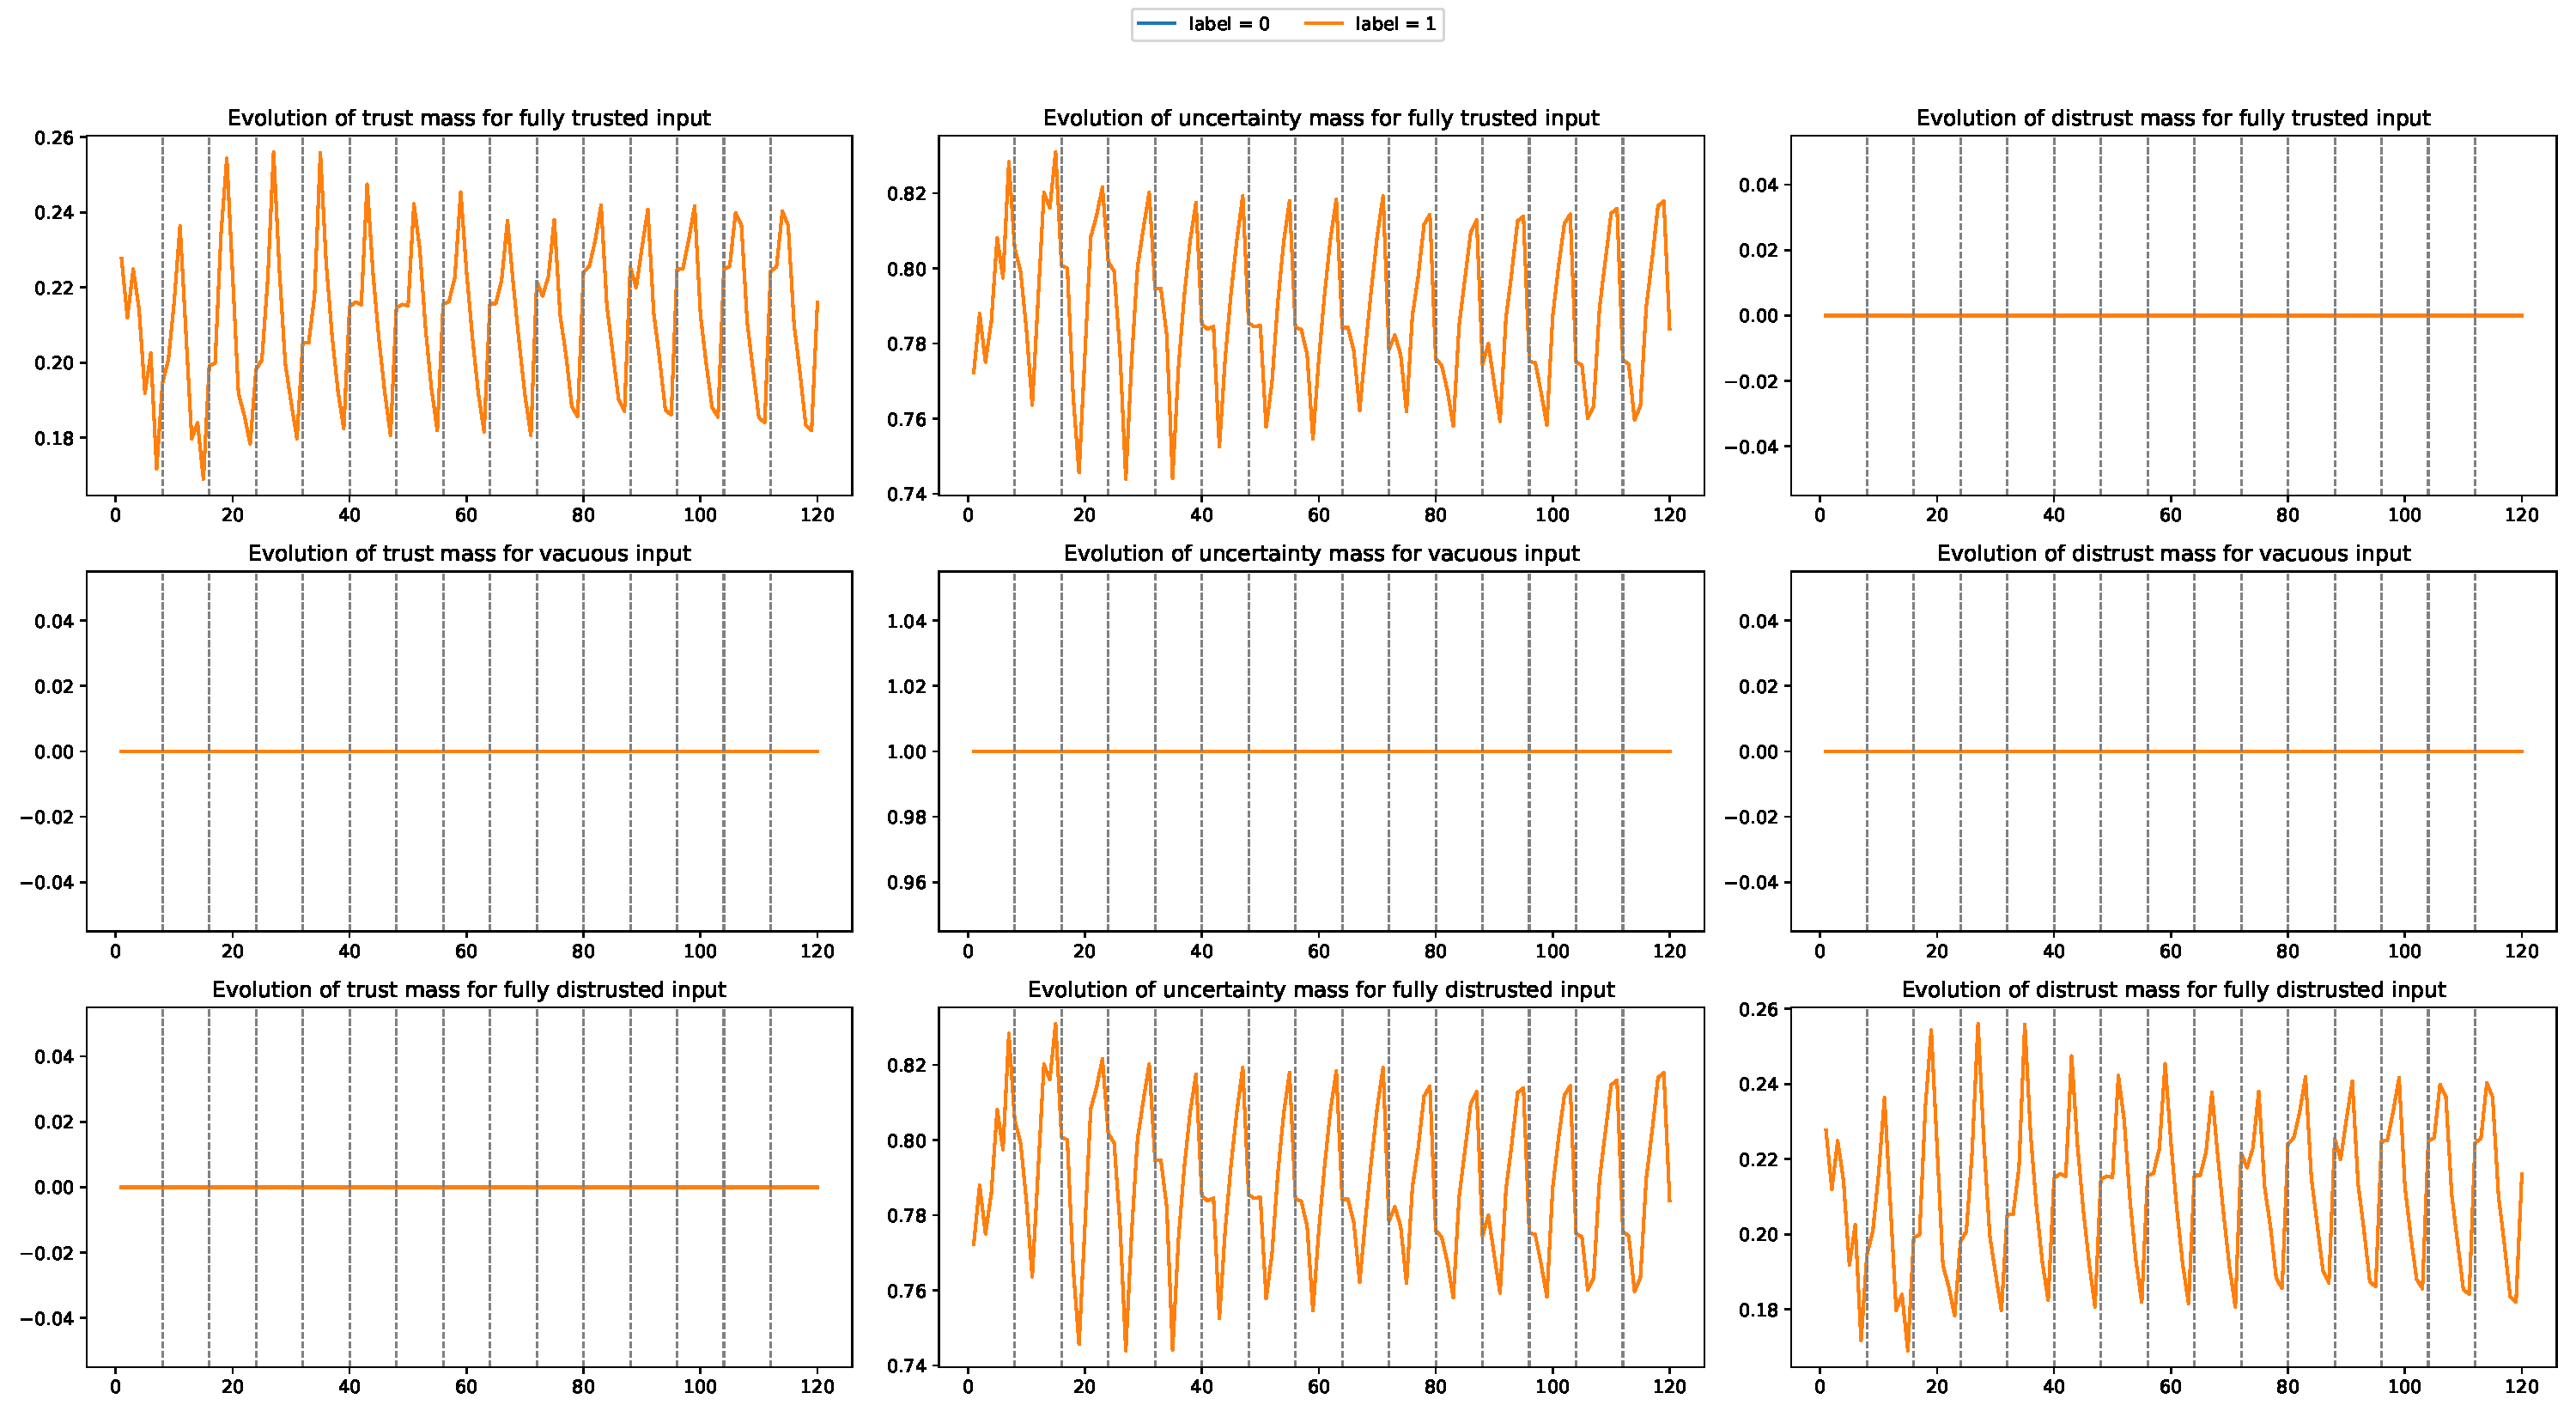
\includegraphics[width=0.8\textwidth]{latex/PTAS_Eval_cancer_16_0.25_0.0_0.75_0.25_0.0_0.75_eps_0.01_PathSize_None__plot_ptas.pdf}
\caption{cancer\_16\_0.25,0.0,0.75\_0.25,0.0,0.75, $\varepsilon$=0.01}
\end{figure}

\begin{figure}[htbp]
\centering
  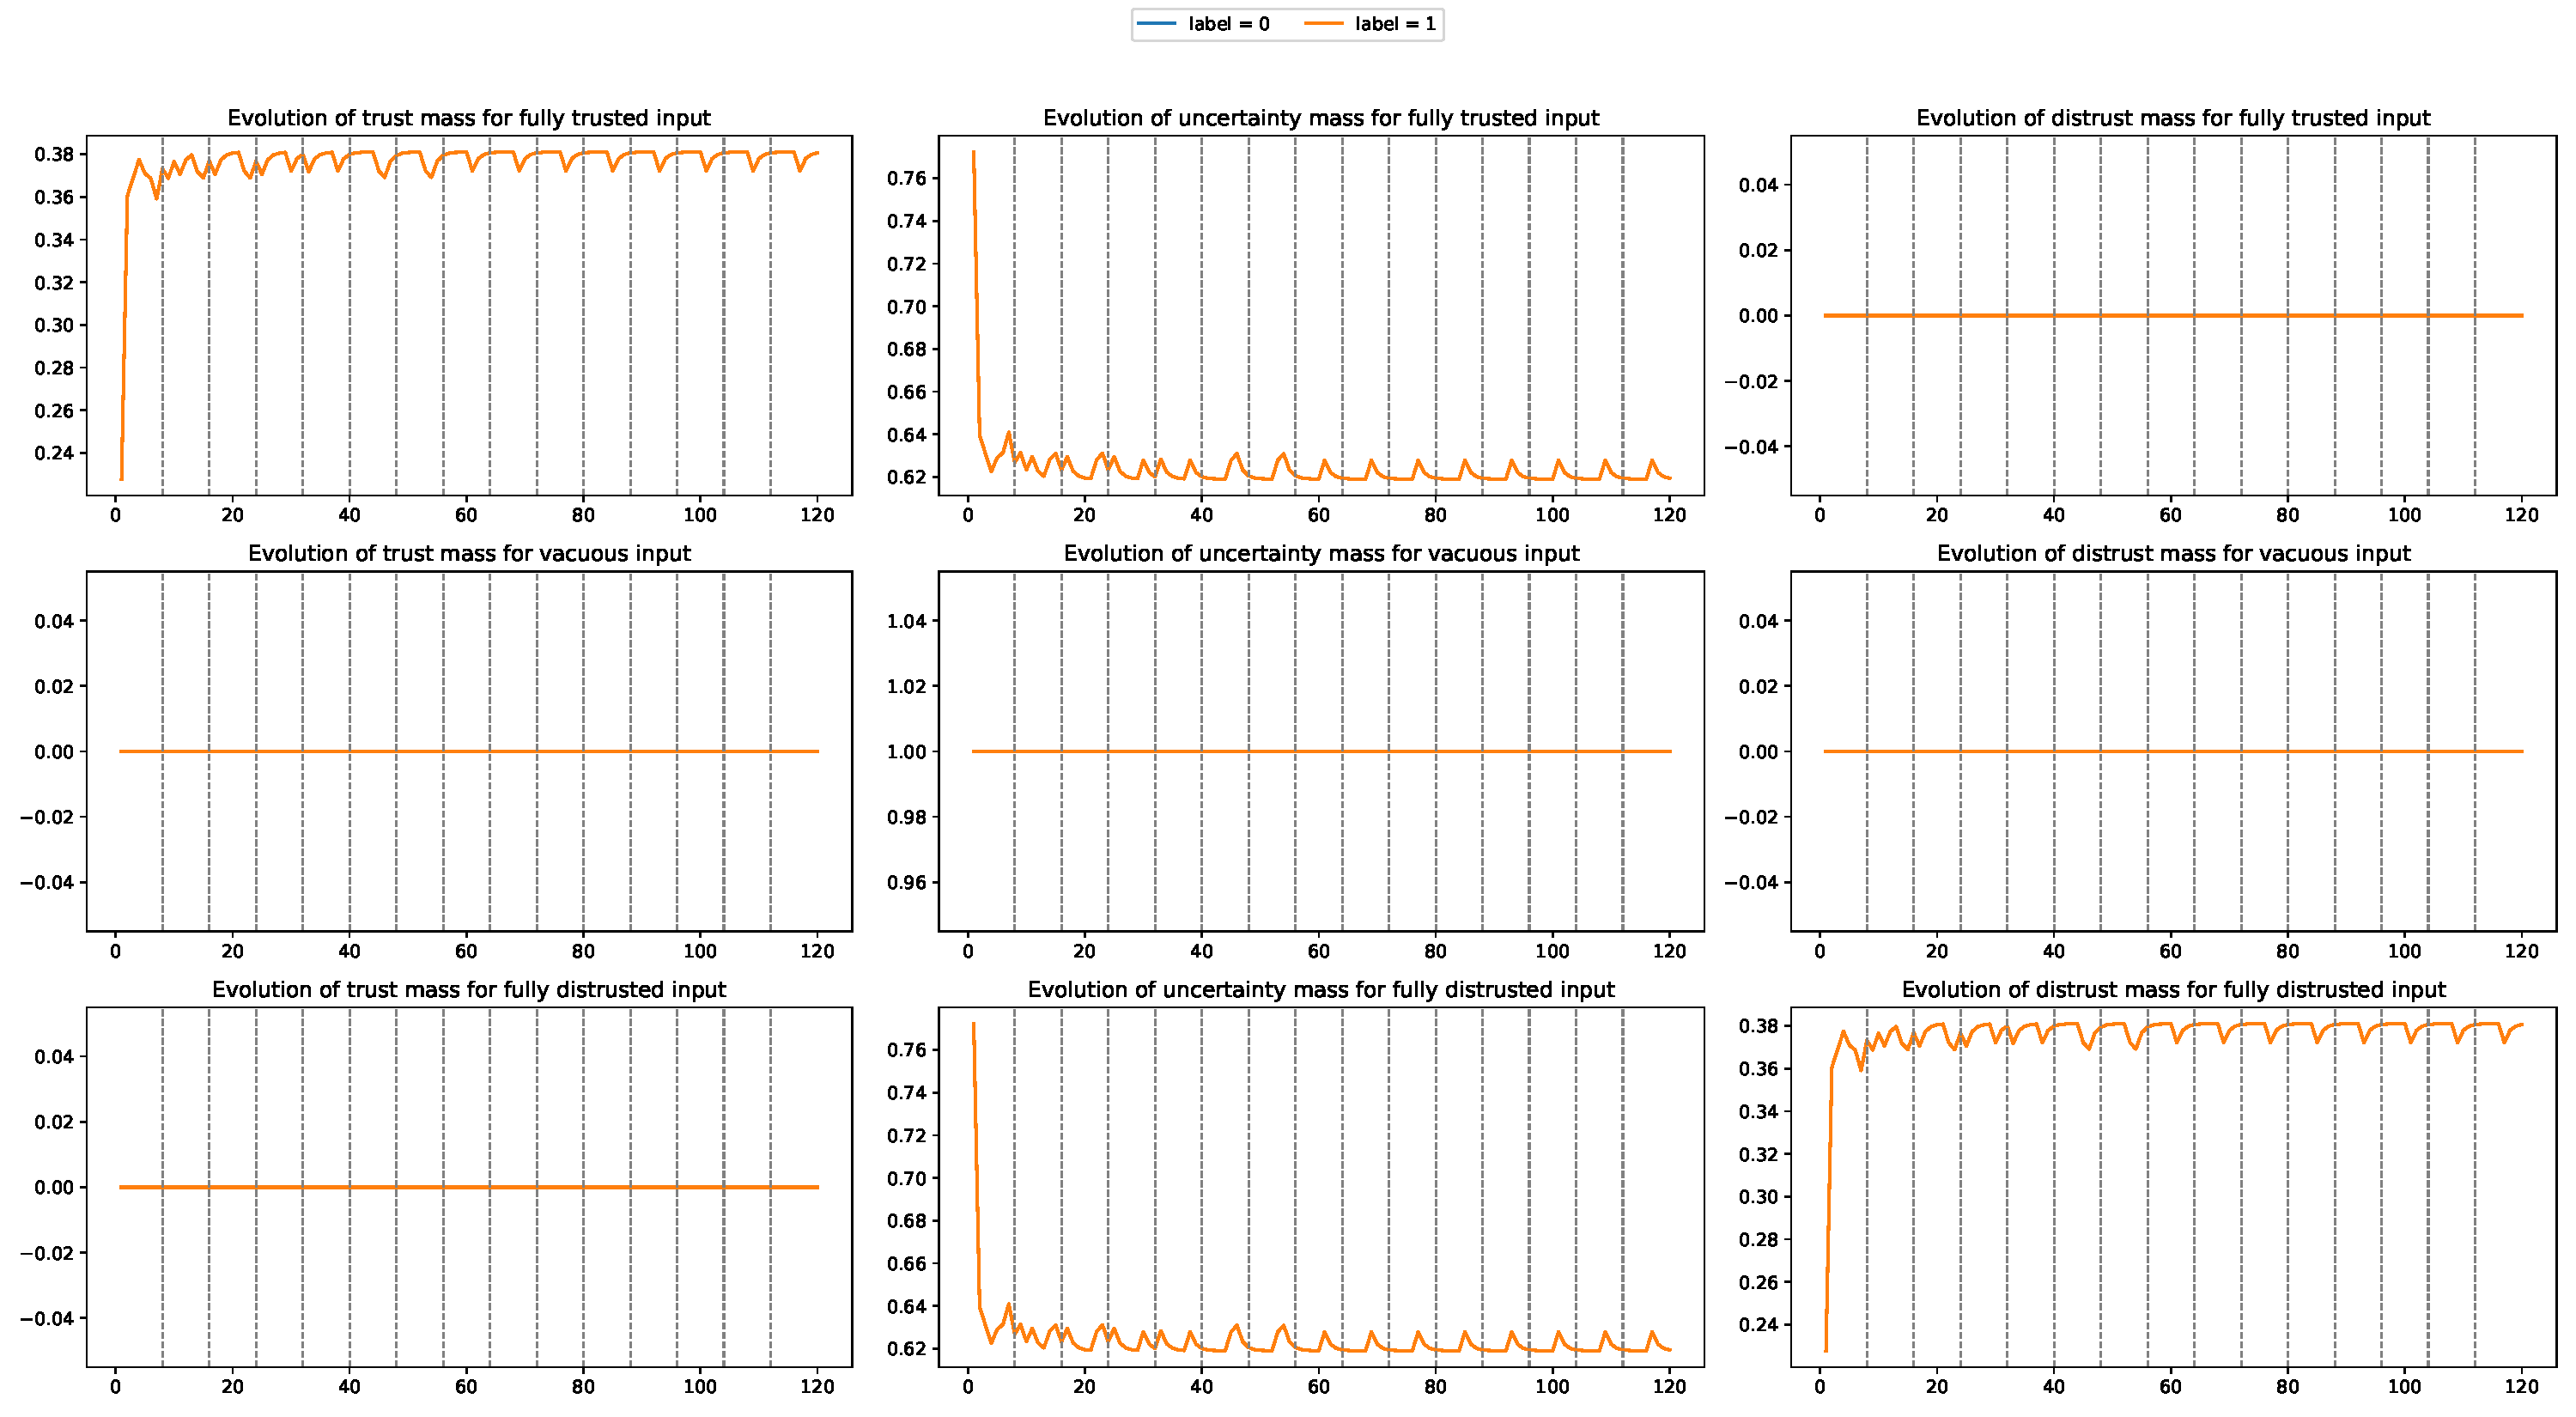
\includegraphics[width=0.8\textwidth]{latex/PTAS_Eval_cancer_16_0.25_0.0_0.75_0.25_0.0_0.75_eps_0.1_PathSize_None__plot_ptas.pdf}
\caption{cancer\_16\_0.25,0.0,0.75\_0.25,0.0,0.75, $\varepsilon$=0.1}
\end{figure}

\begin{figure}[htbp]
\centering
  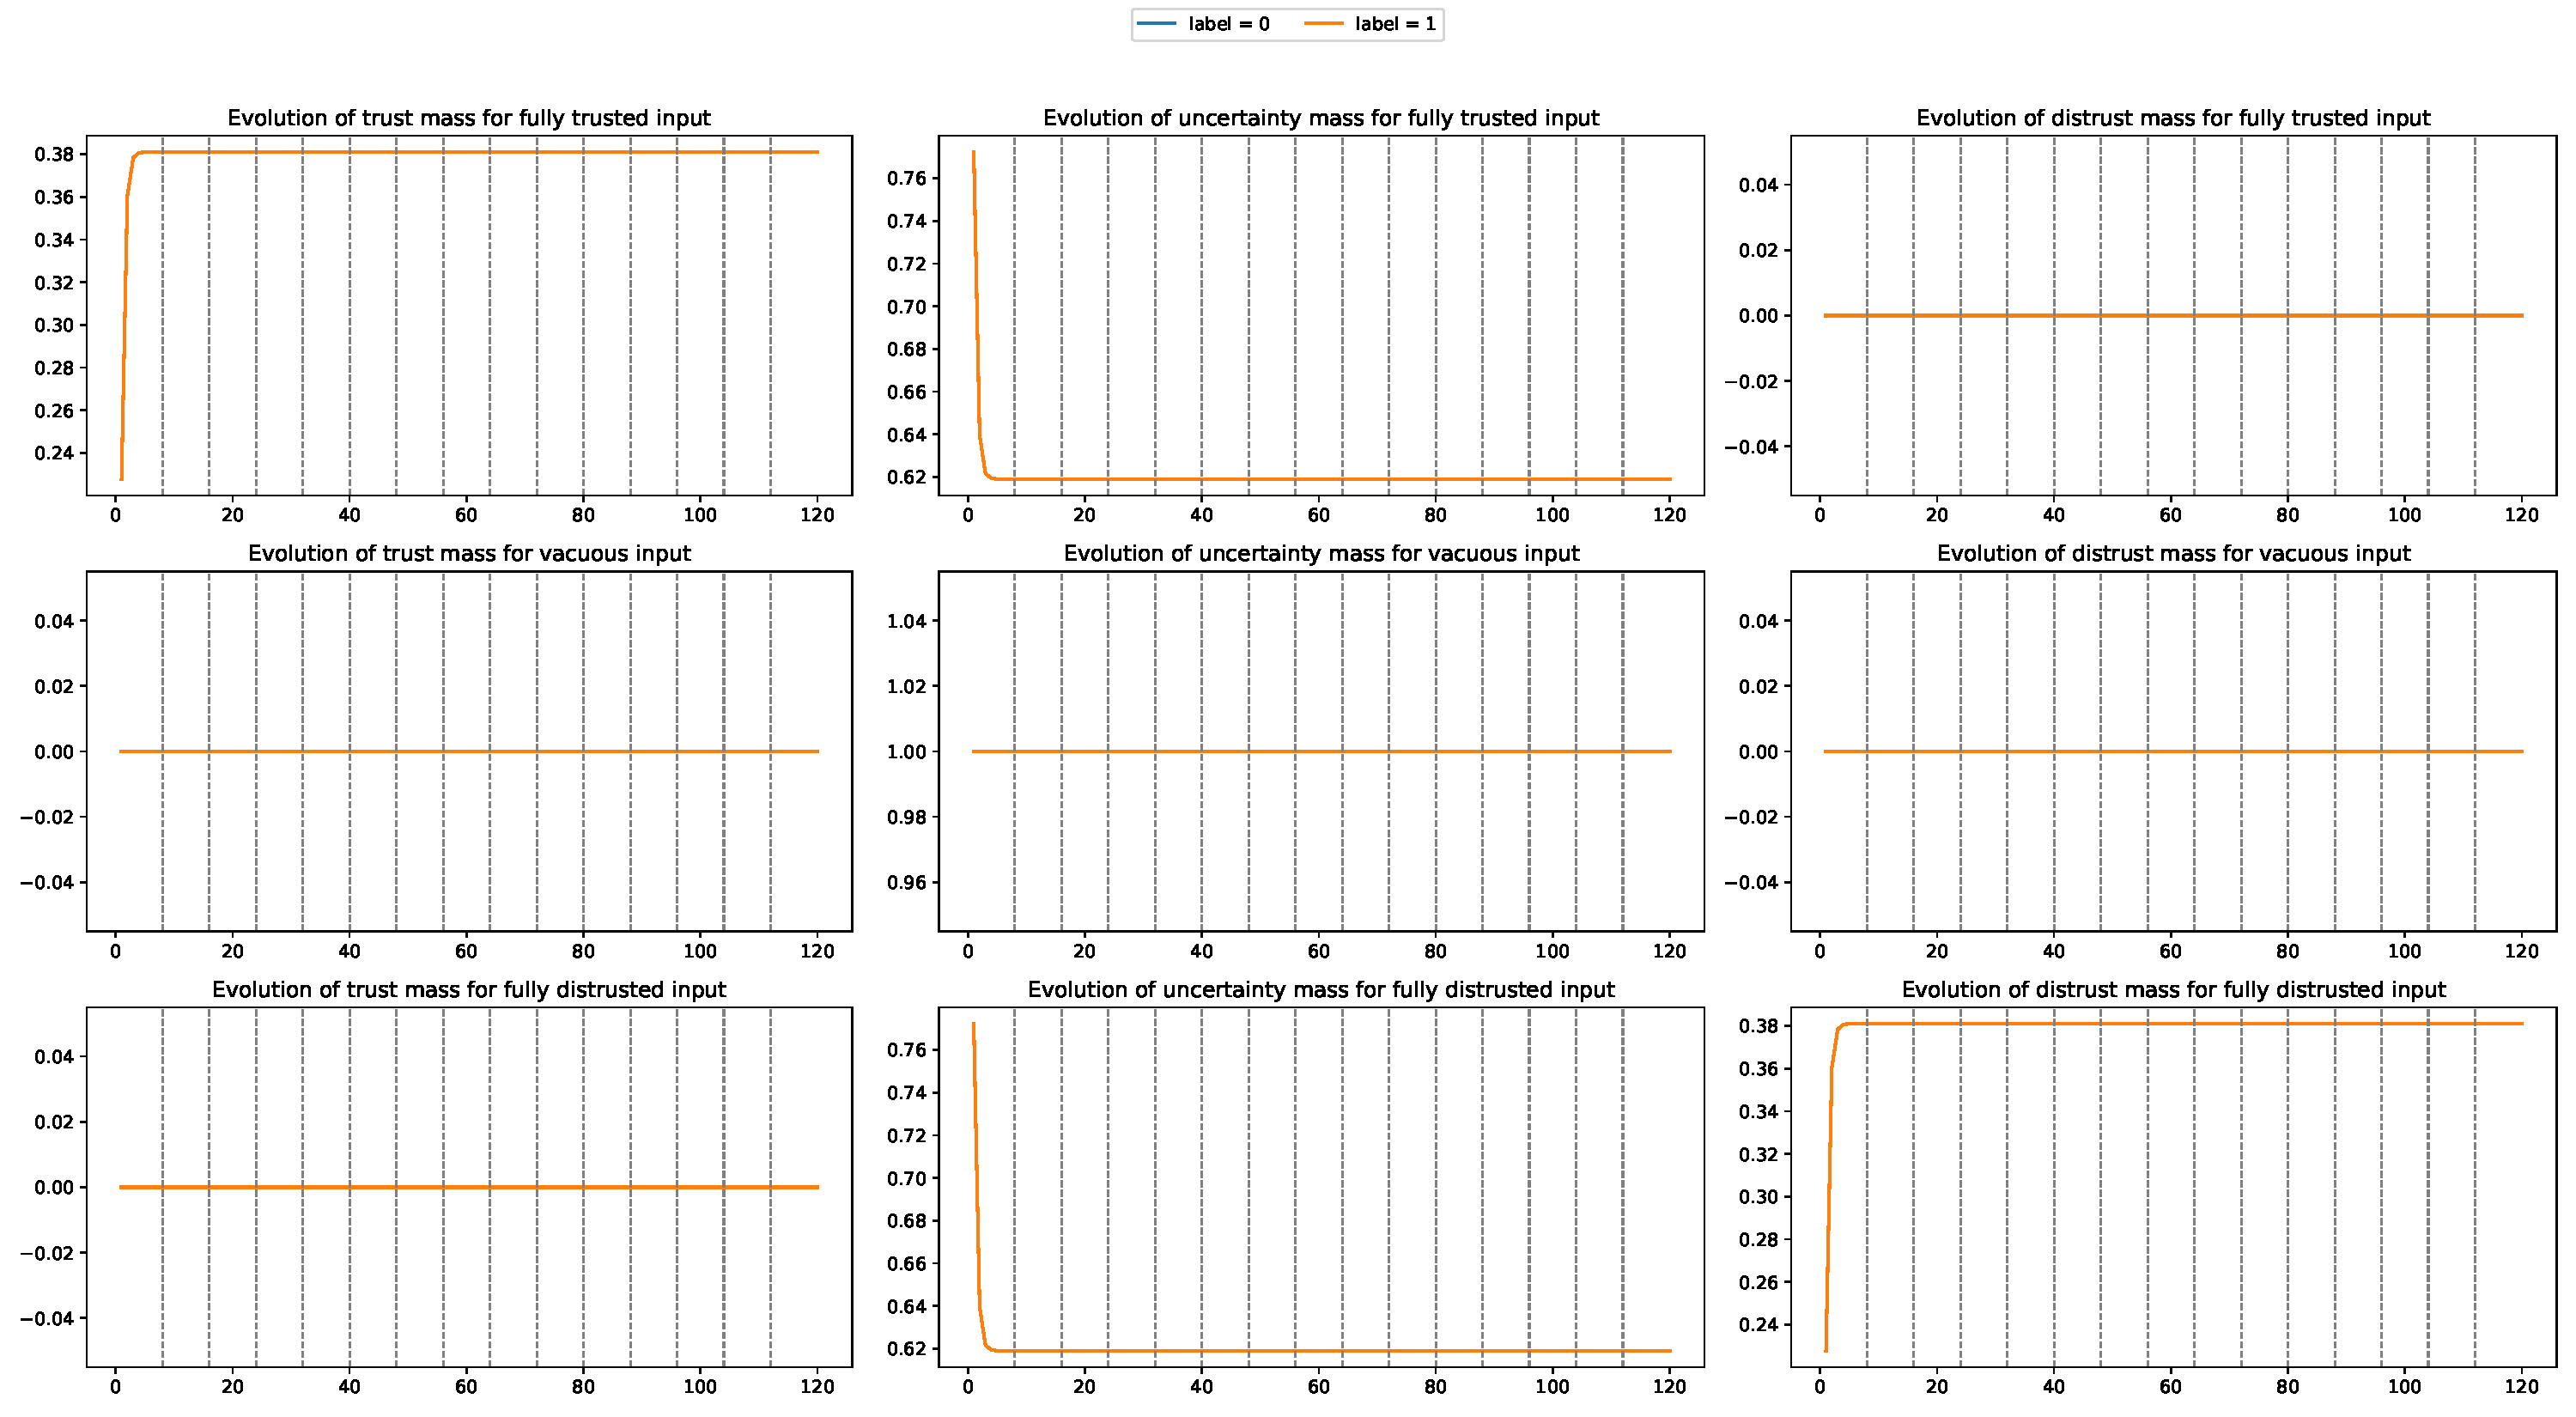
\includegraphics[width=0.8\textwidth]{latex/PTAS_Eval_cancer_16_0.25_0.0_0.75_0.25_0.0_0.75_eps_1_PathSize_None__plot_ptas.pdf}
\caption{cancer\_16\_0.25,0.0,0.75\_0.25,0.0,0.75, $\varepsilon$=1}
\end{figure}

\subsubsection{(0.25, 0.25, 0.5) -- (0.25, 0.25, 0.5)}

\begin{figure}[htbp]
\centering
  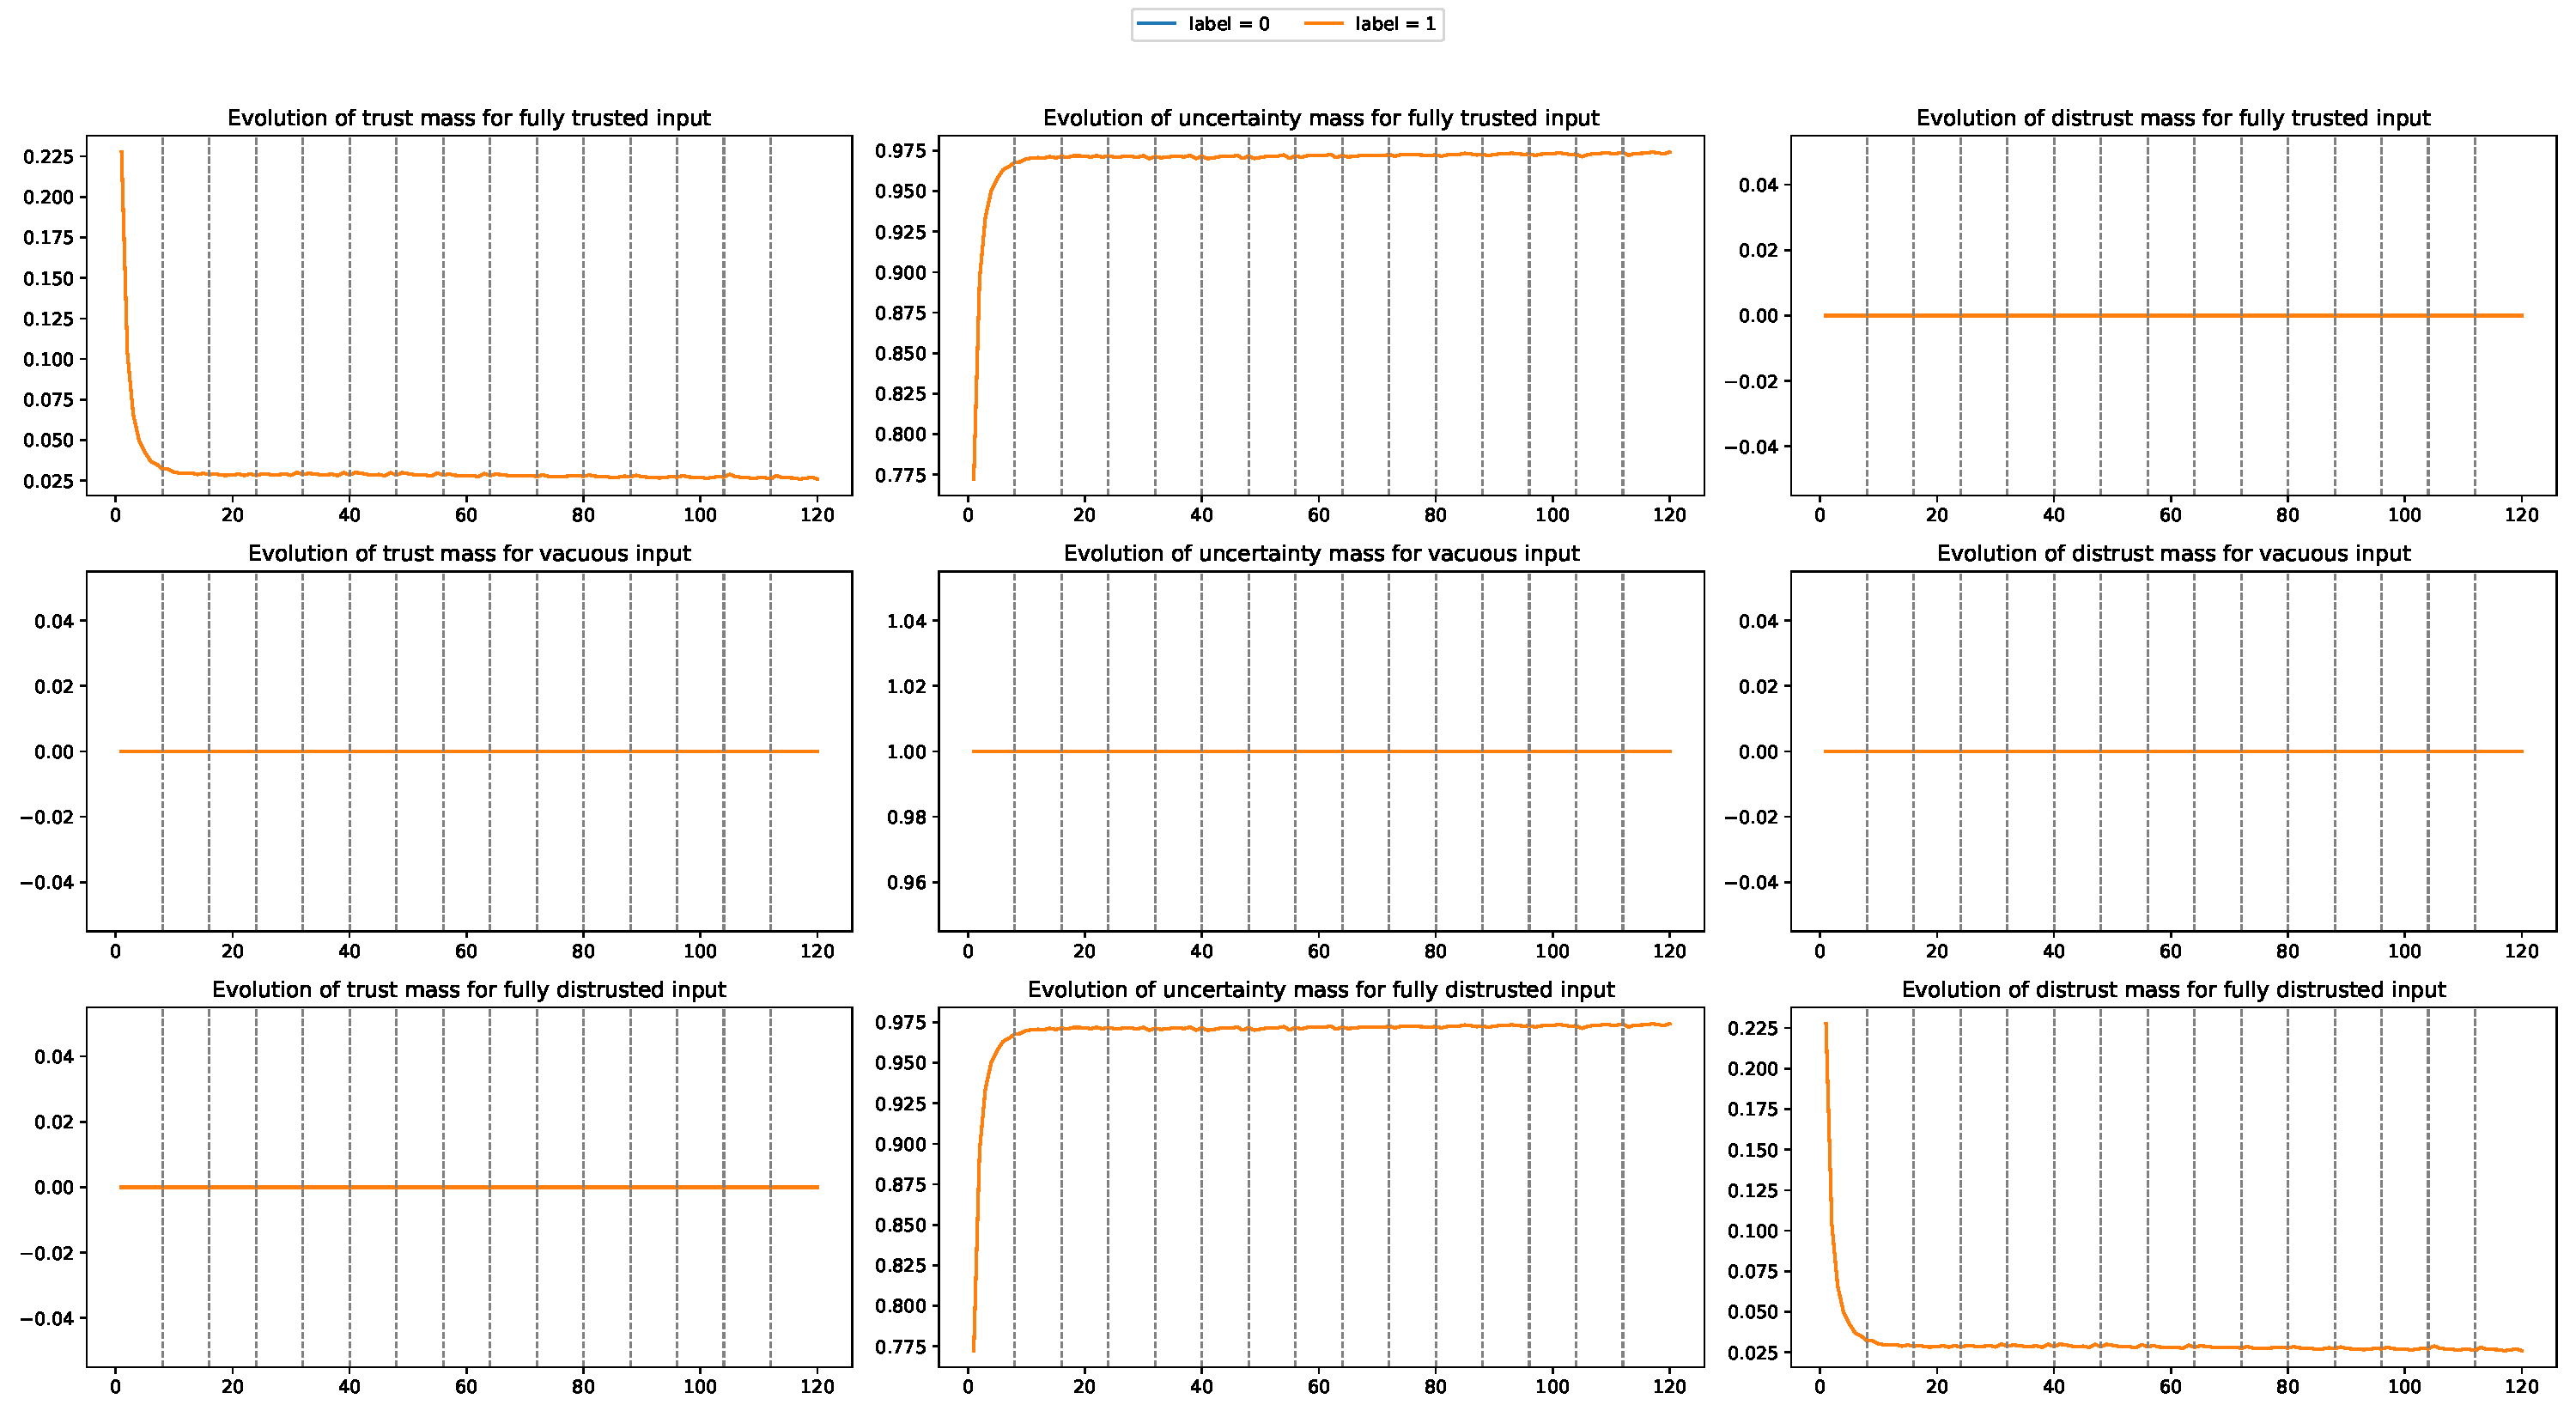
\includegraphics[width=0.8\textwidth]{latex/PTAS_Eval_cancer_16_0.25_0.25_0.5_0.25_0.25_0.5_eps_0.001_PathSize_None__plot_ptas.pdf}
\caption{cancer\_16\_0.25,0.25,0.5\_0.25,0.25,0.5, $\varepsilon$=0.001}
\end{figure}

\begin{figure}[htbp]
\centering
  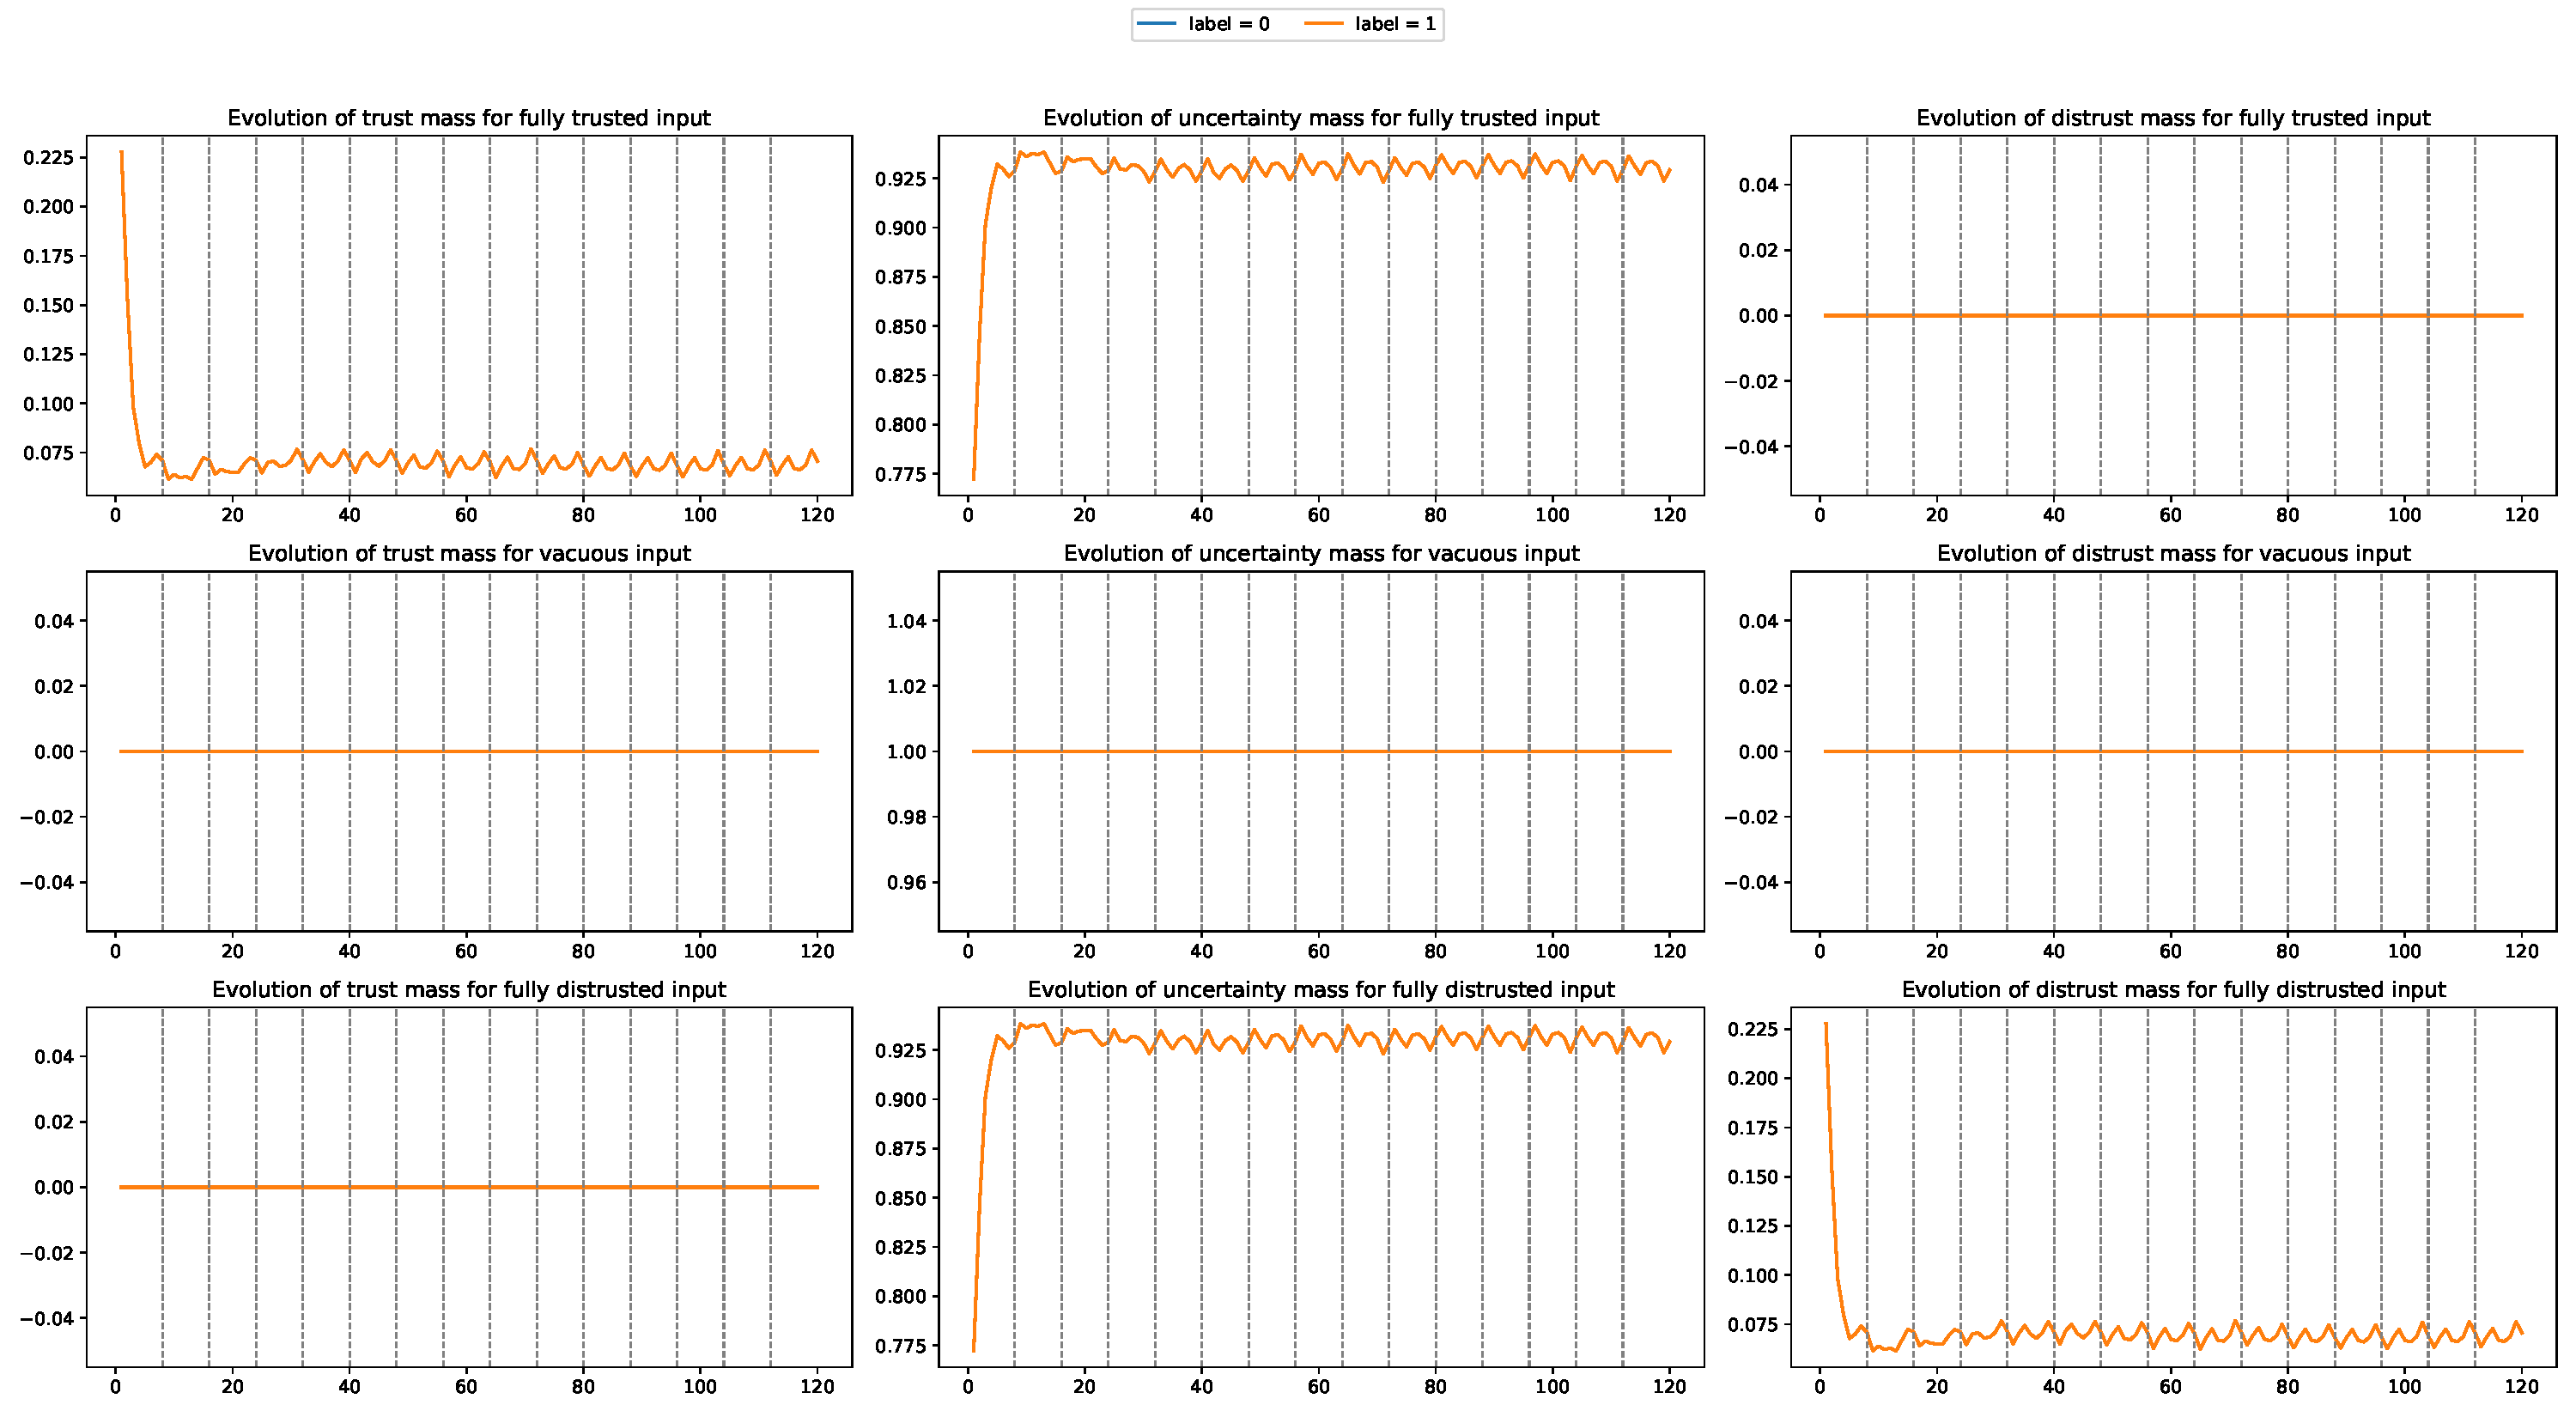
\includegraphics[width=0.8\textwidth]{latex/PTAS_Eval_cancer_16_0.25_0.25_0.5_0.25_0.25_0.5_eps_0.01_PathSize_None__plot_ptas.pdf}
\caption{cancer\_16\_0.25,0.25,0.5\_0.25,0.25,0.5, $\varepsilon$=0.01}
\end{figure}

\begin{figure}[htbp]
\centering
  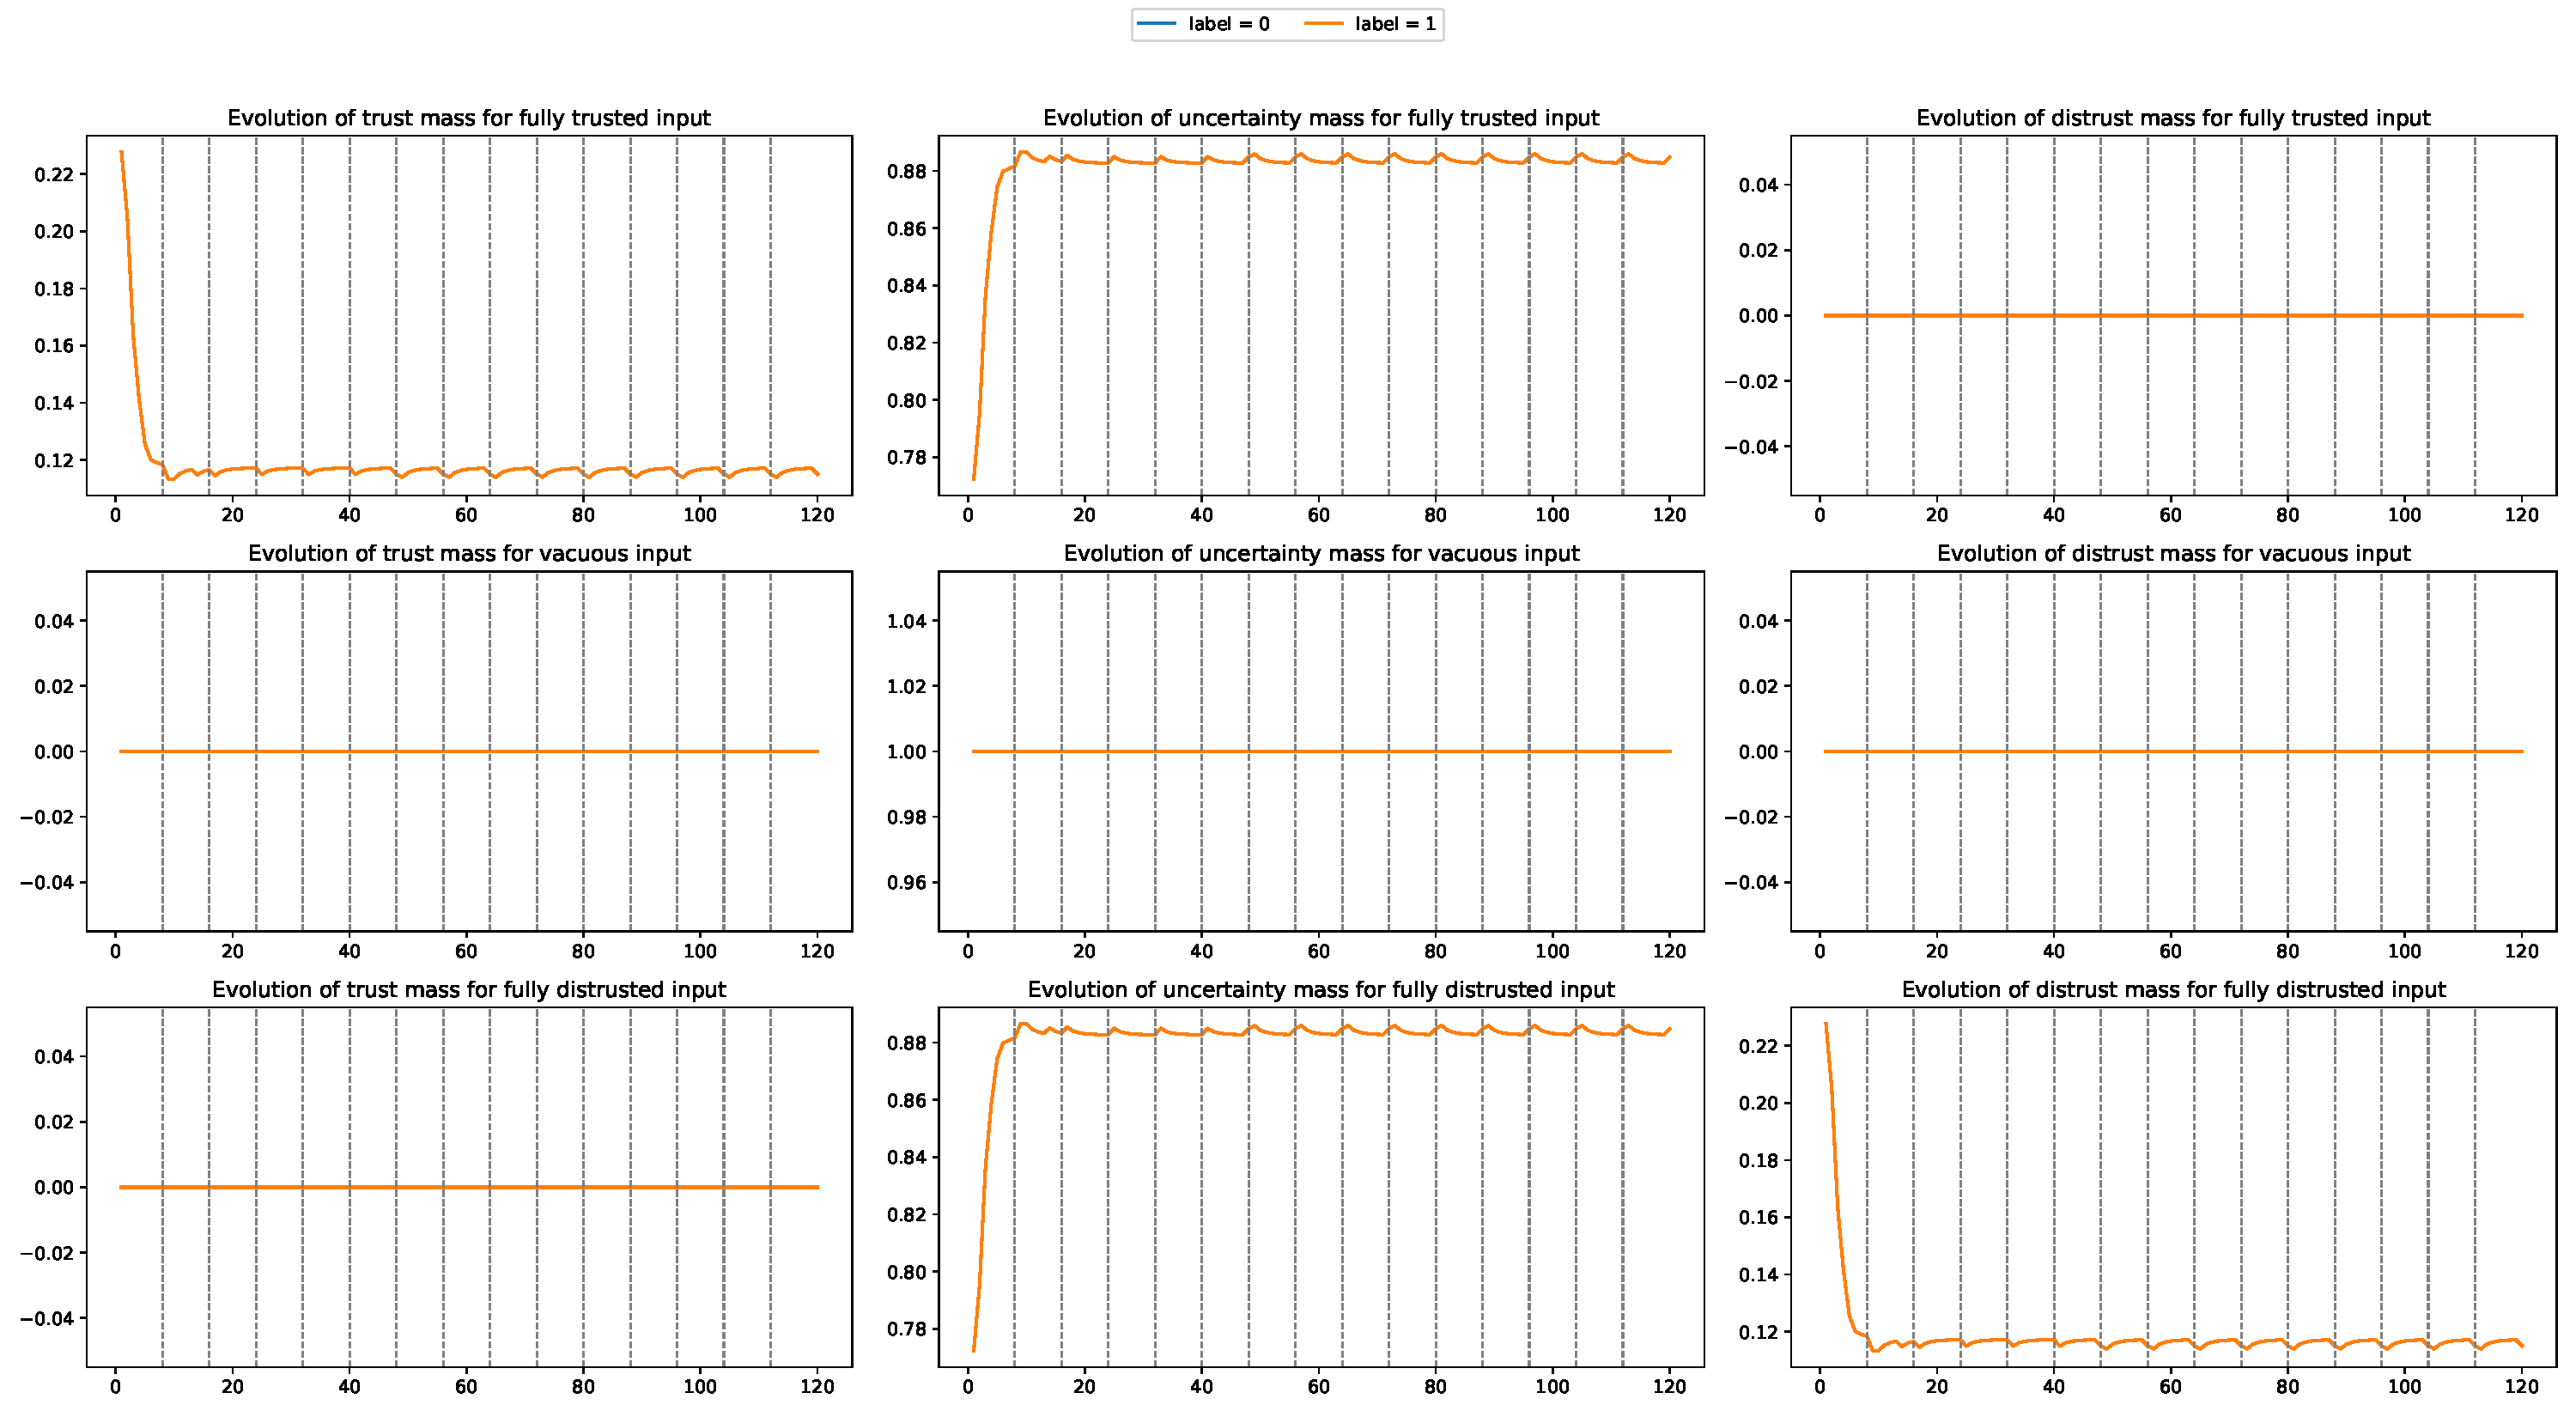
\includegraphics[width=0.8\textwidth]{latex/PTAS_Eval_cancer_16_0.25_0.25_0.5_0.25_0.25_0.5_eps_0.1_PathSize_None__plot_ptas.pdf}
\caption{cancer\_16\_0.25,0.25,0.5\_0.25,0.25,0.5, $\varepsilon$=0.1}
\end{figure}

\begin{figure}[htbp]
\centering
  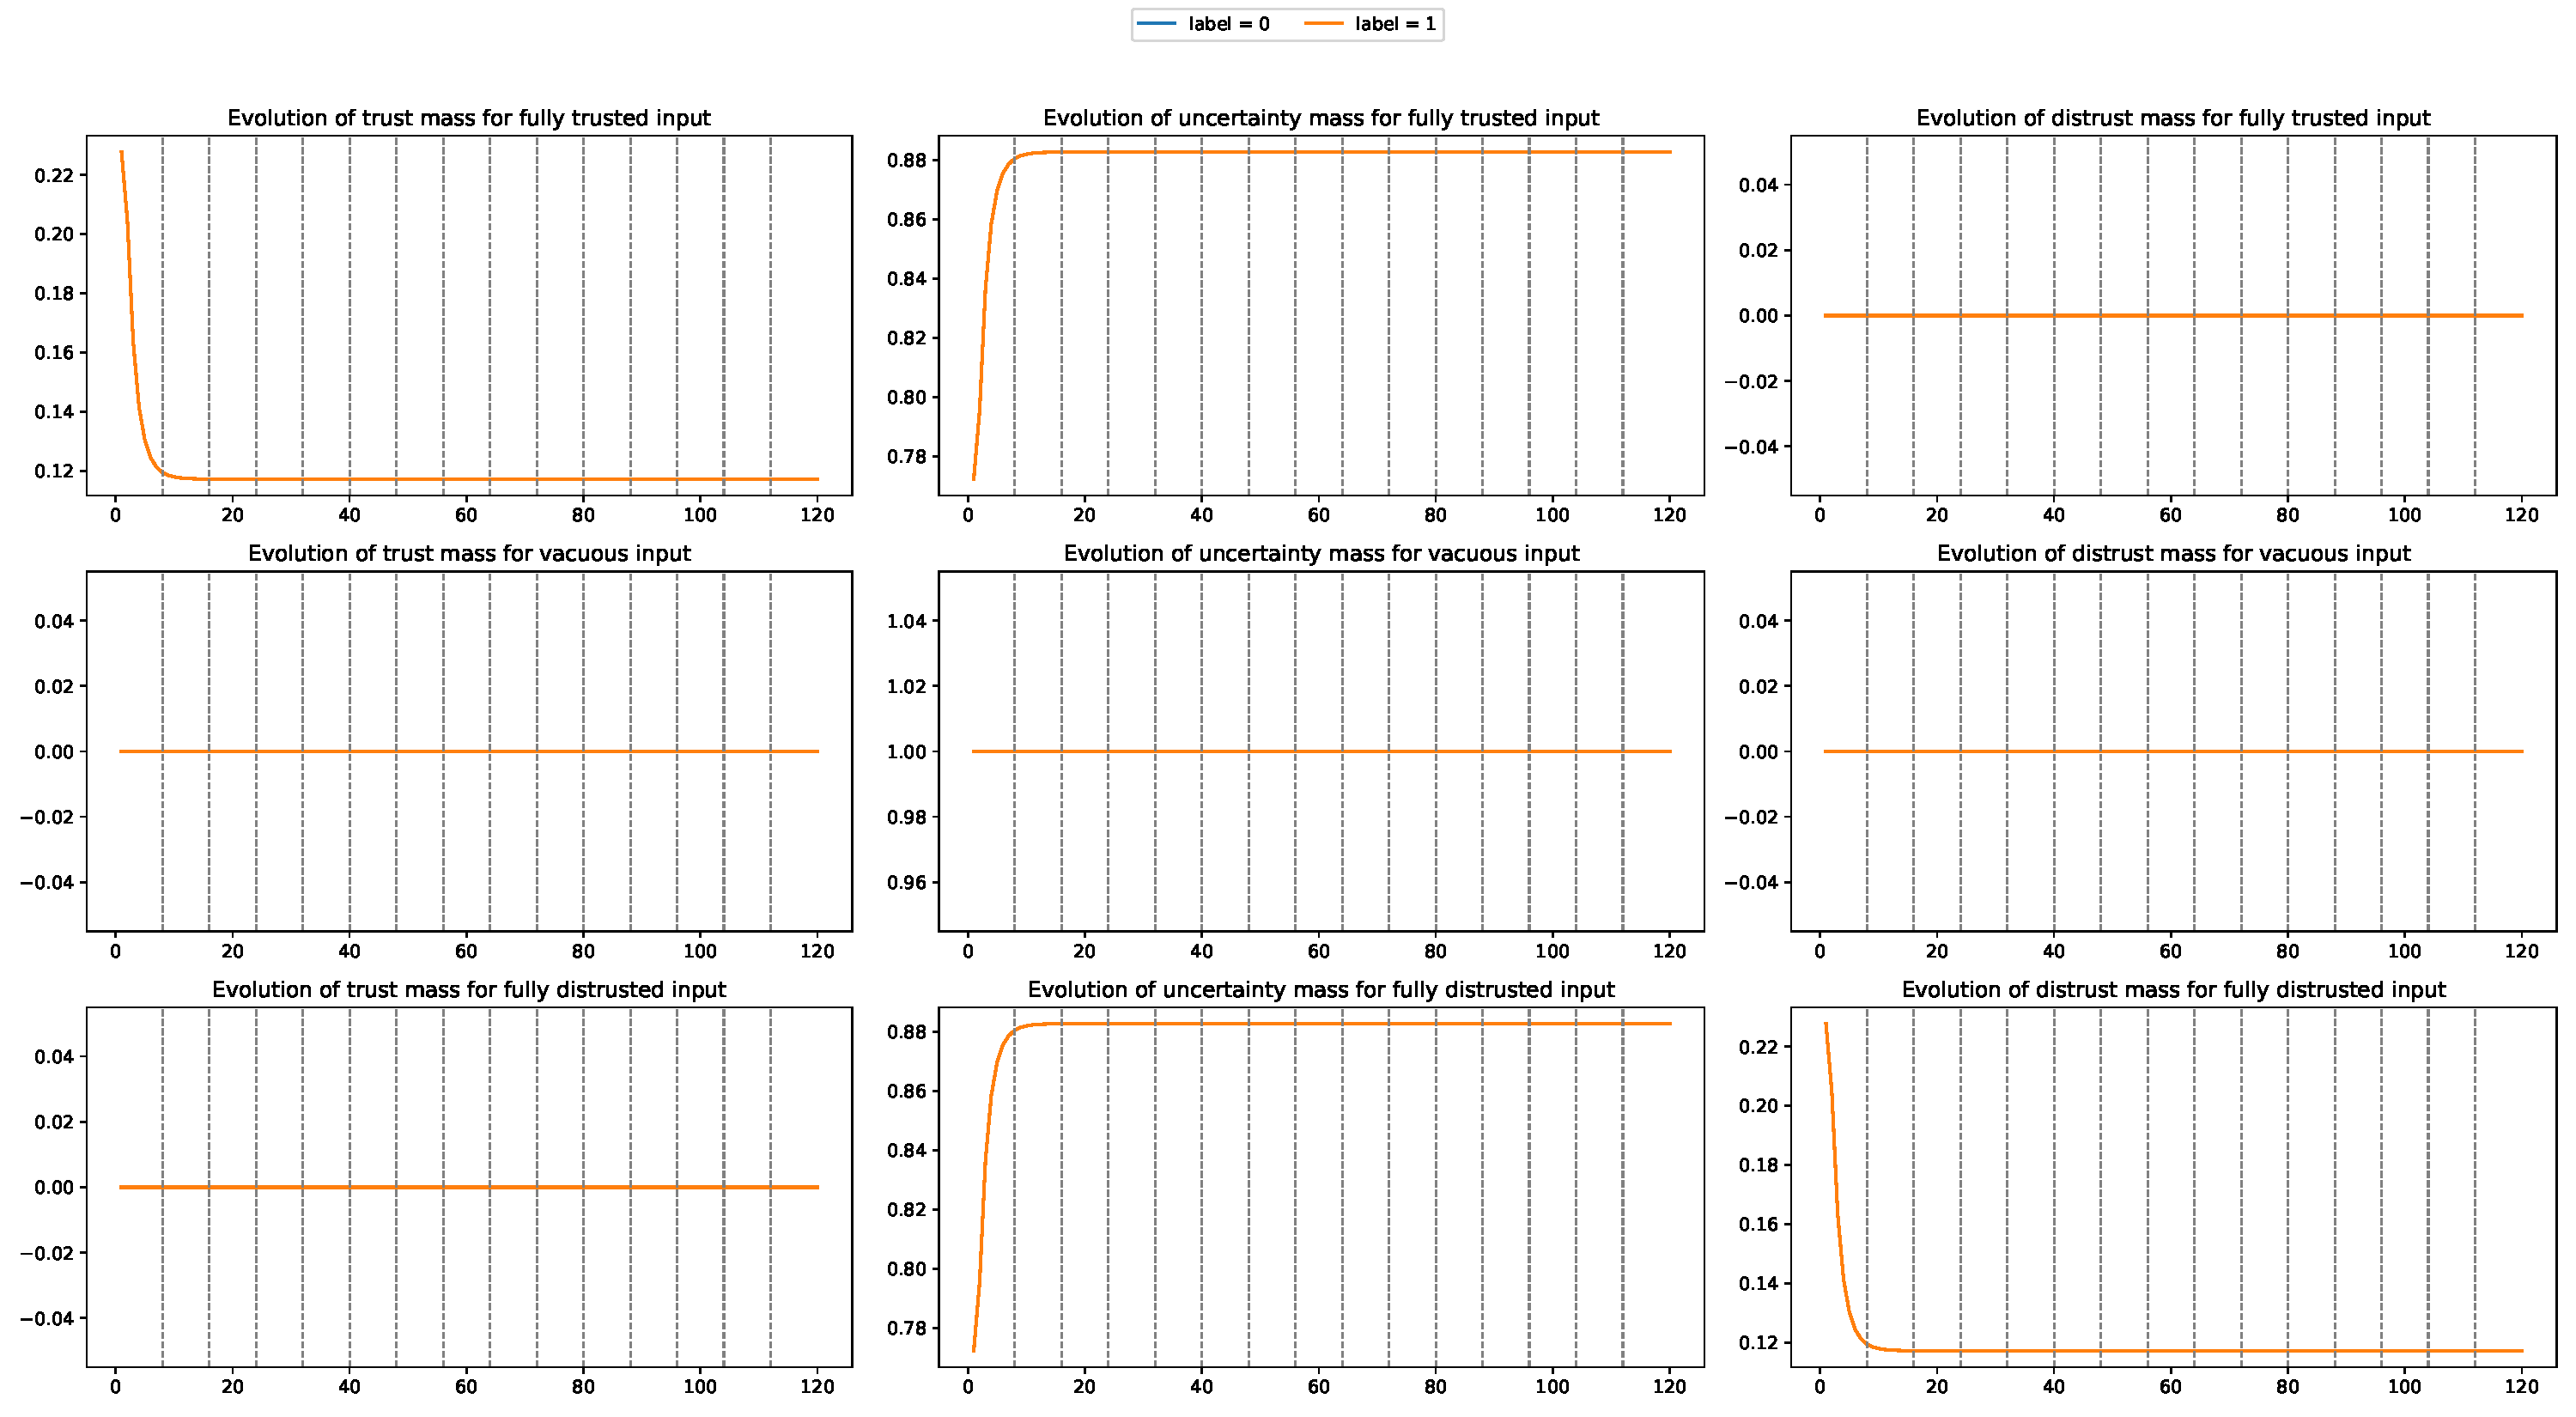
\includegraphics[width=0.8\textwidth]{latex/PTAS_Eval_cancer_16_0.25_0.25_0.5_0.25_0.25_0.5_eps_1_PathSize_None__plot_ptas.pdf}
\caption{cancer\_16\_0.25,0.25,0.5\_0.25,0.25,0.5, $\varepsilon$=1}
\end{figure}

\subsubsection{distrust -- distrust}

\begin{figure}[htbp]
\centering
  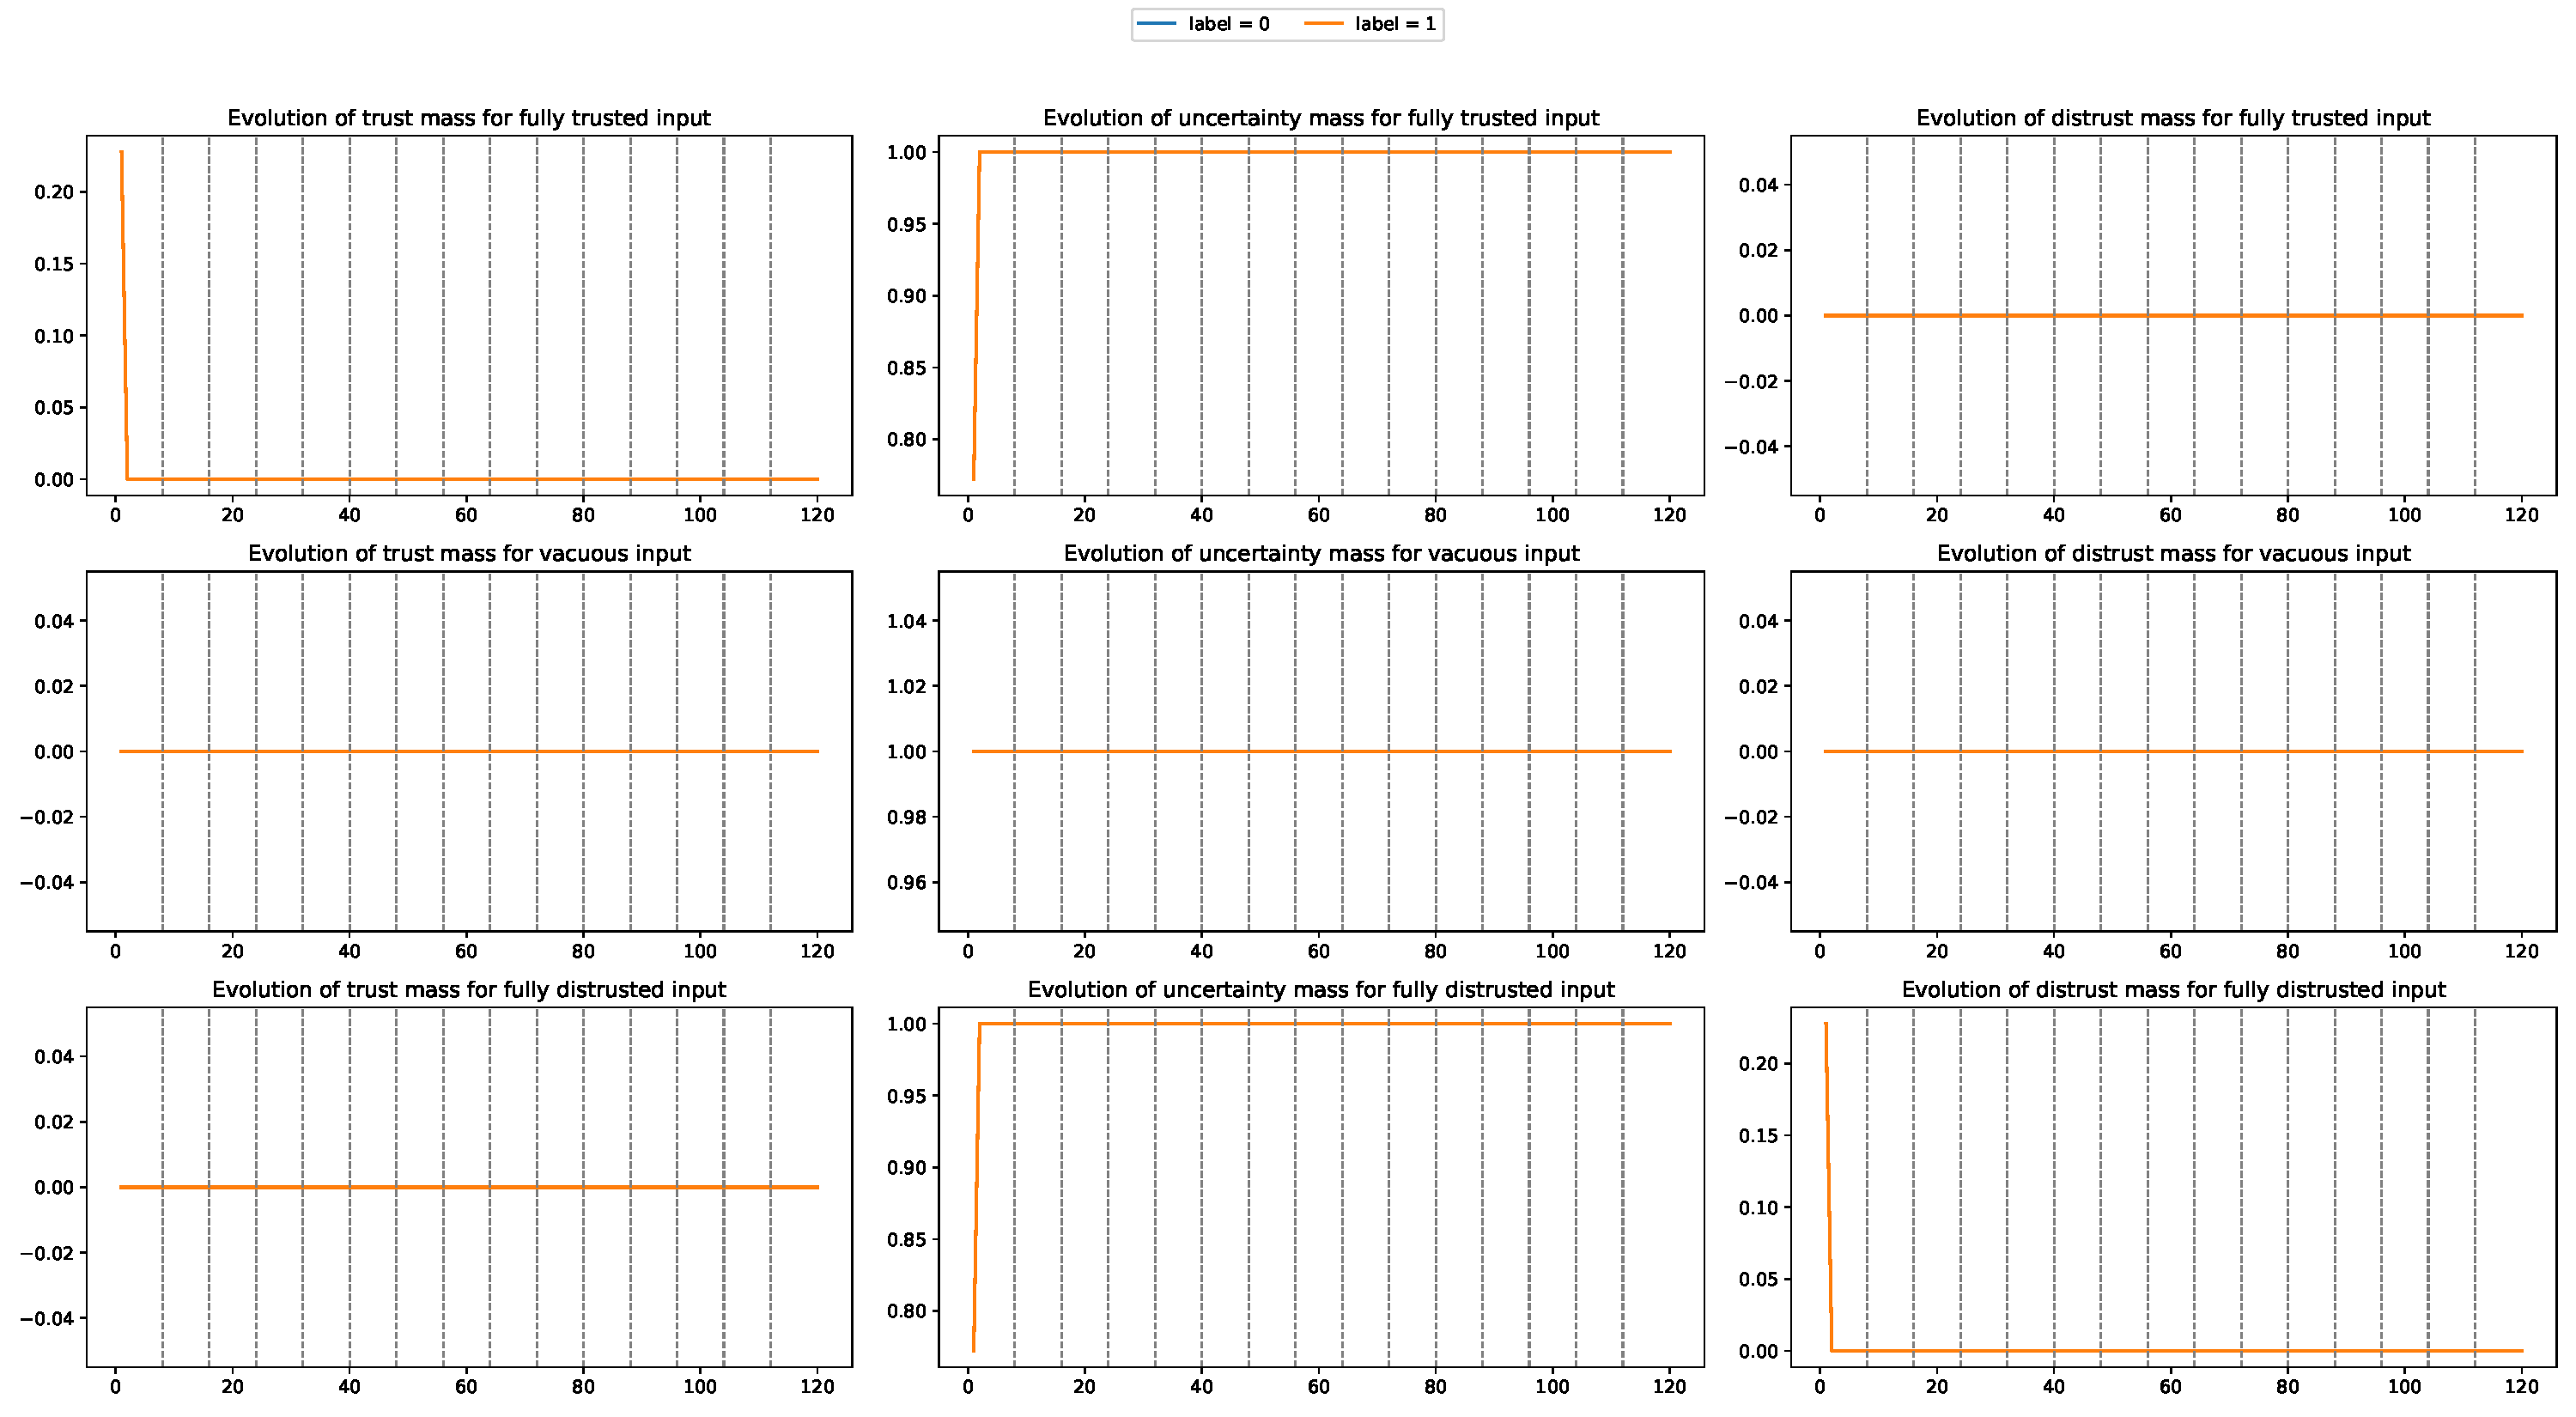
\includegraphics[width=0.8\textwidth]{latex/PTAS_Eval_cancer_16_distrust_distrust_eps_0.001_PathSize_None__plot_ptas.pdf}
\caption{cancer\_16\_distrust\_distrust, $\varepsilon$=0.001}
\end{figure}

\begin{figure}[htbp]
\centering
  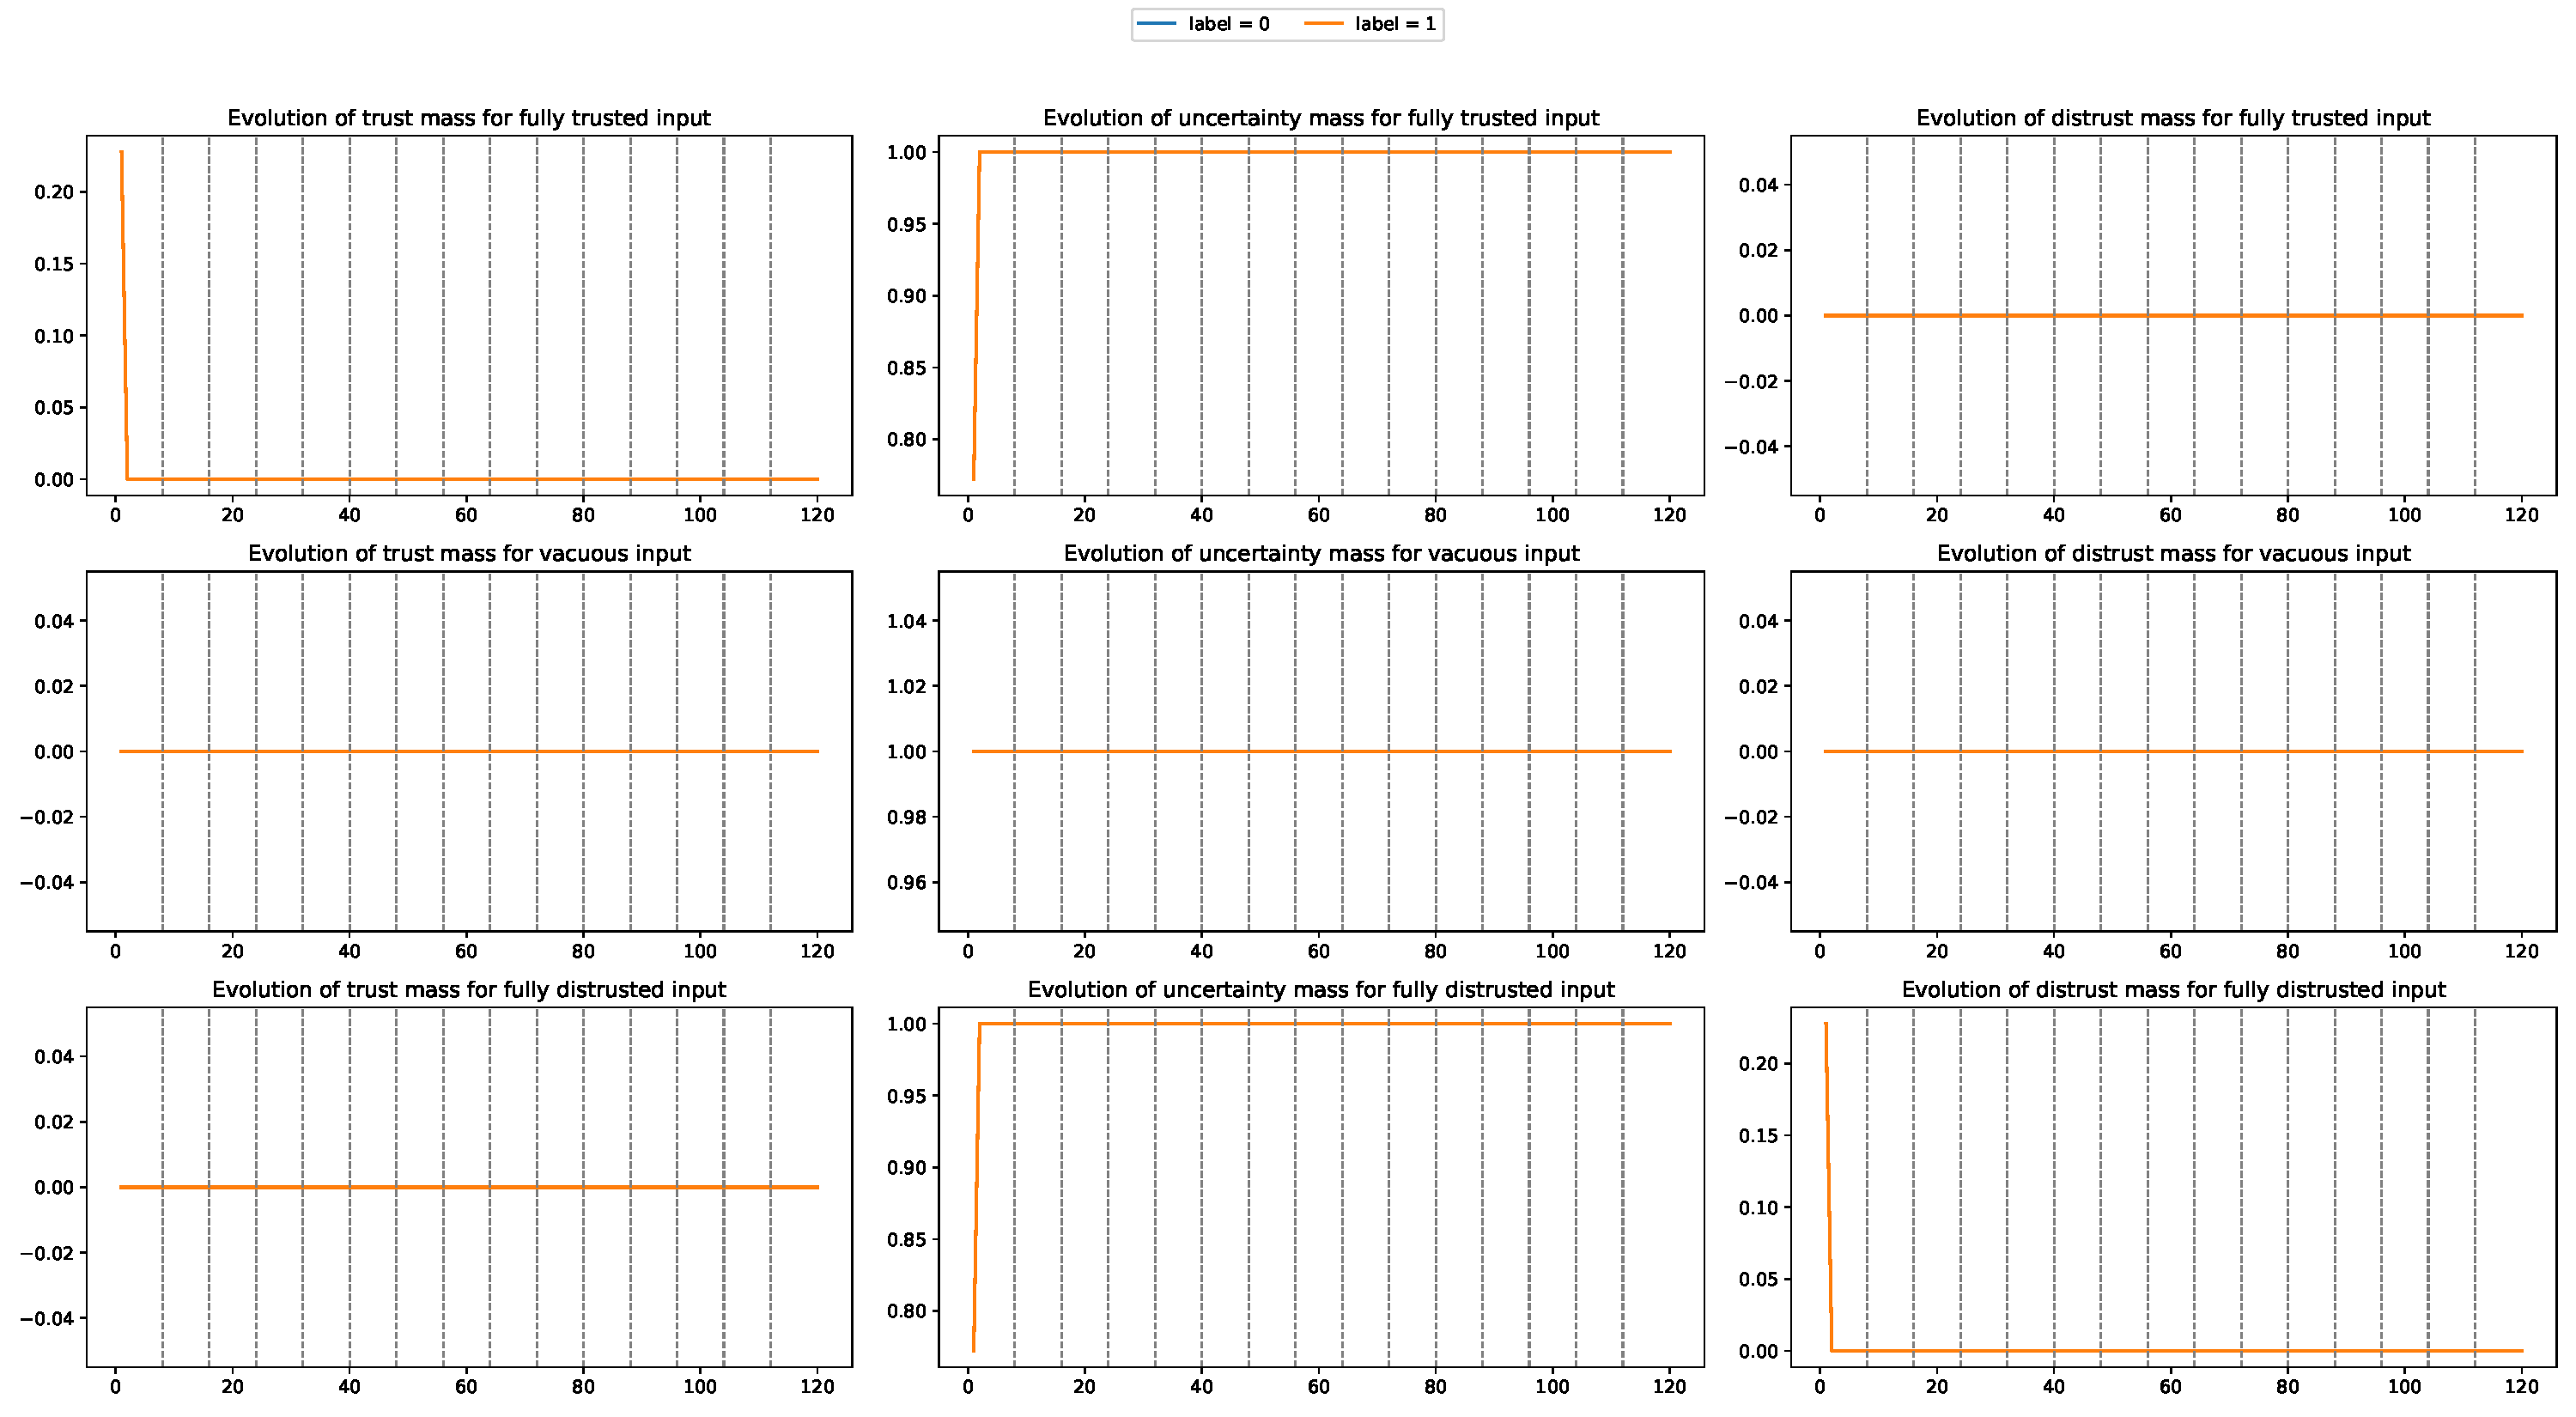
\includegraphics[width=0.8\textwidth]{latex/PTAS_Eval_cancer_16_distrust_distrust_eps_0.01_PathSize_None__plot_ptas.pdf}
\caption{cancer\_16\_distrust\_distrust, $\varepsilon$=0.01}
\end{figure}

\begin{figure}[htbp]
\centering
  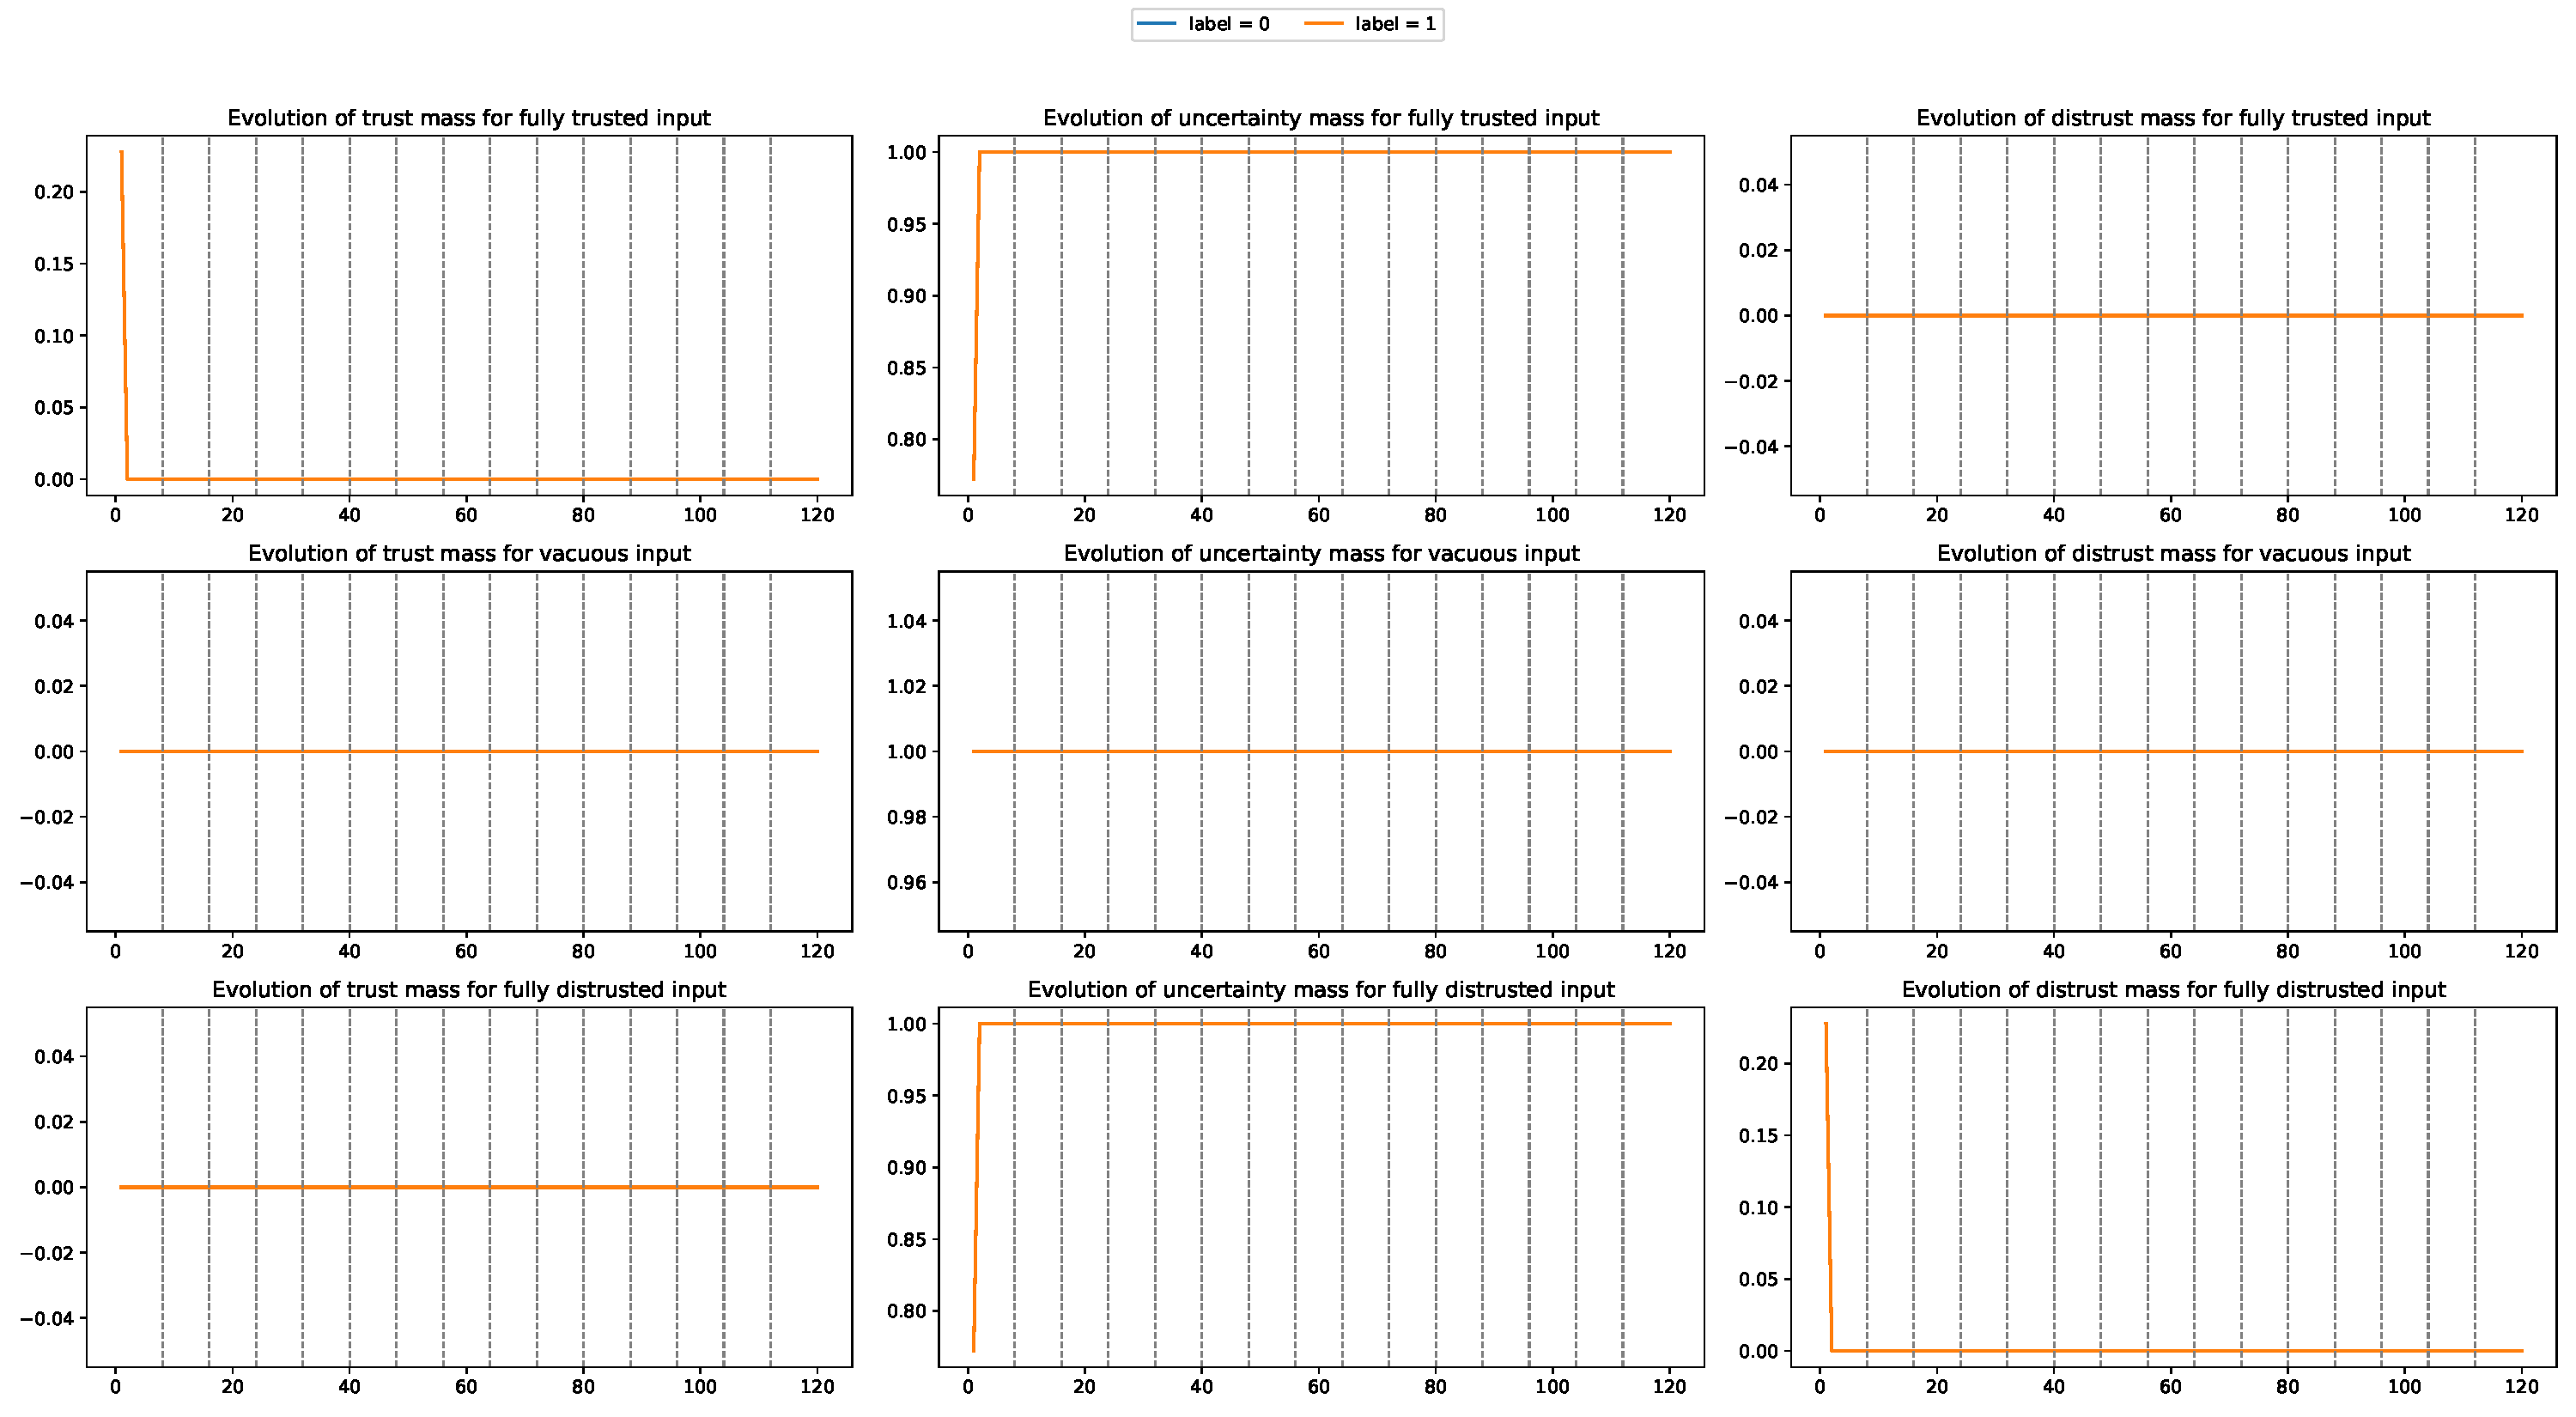
\includegraphics[width=0.8\textwidth]{latex/PTAS_Eval_cancer_16_distrust_distrust_eps_0.1_PathSize_None__plot_ptas.pdf}
\caption{cancer\_16\_distrust\_distrust, $\varepsilon$=0.1}
\end{figure}

\begin{figure}[htbp]
\centering
  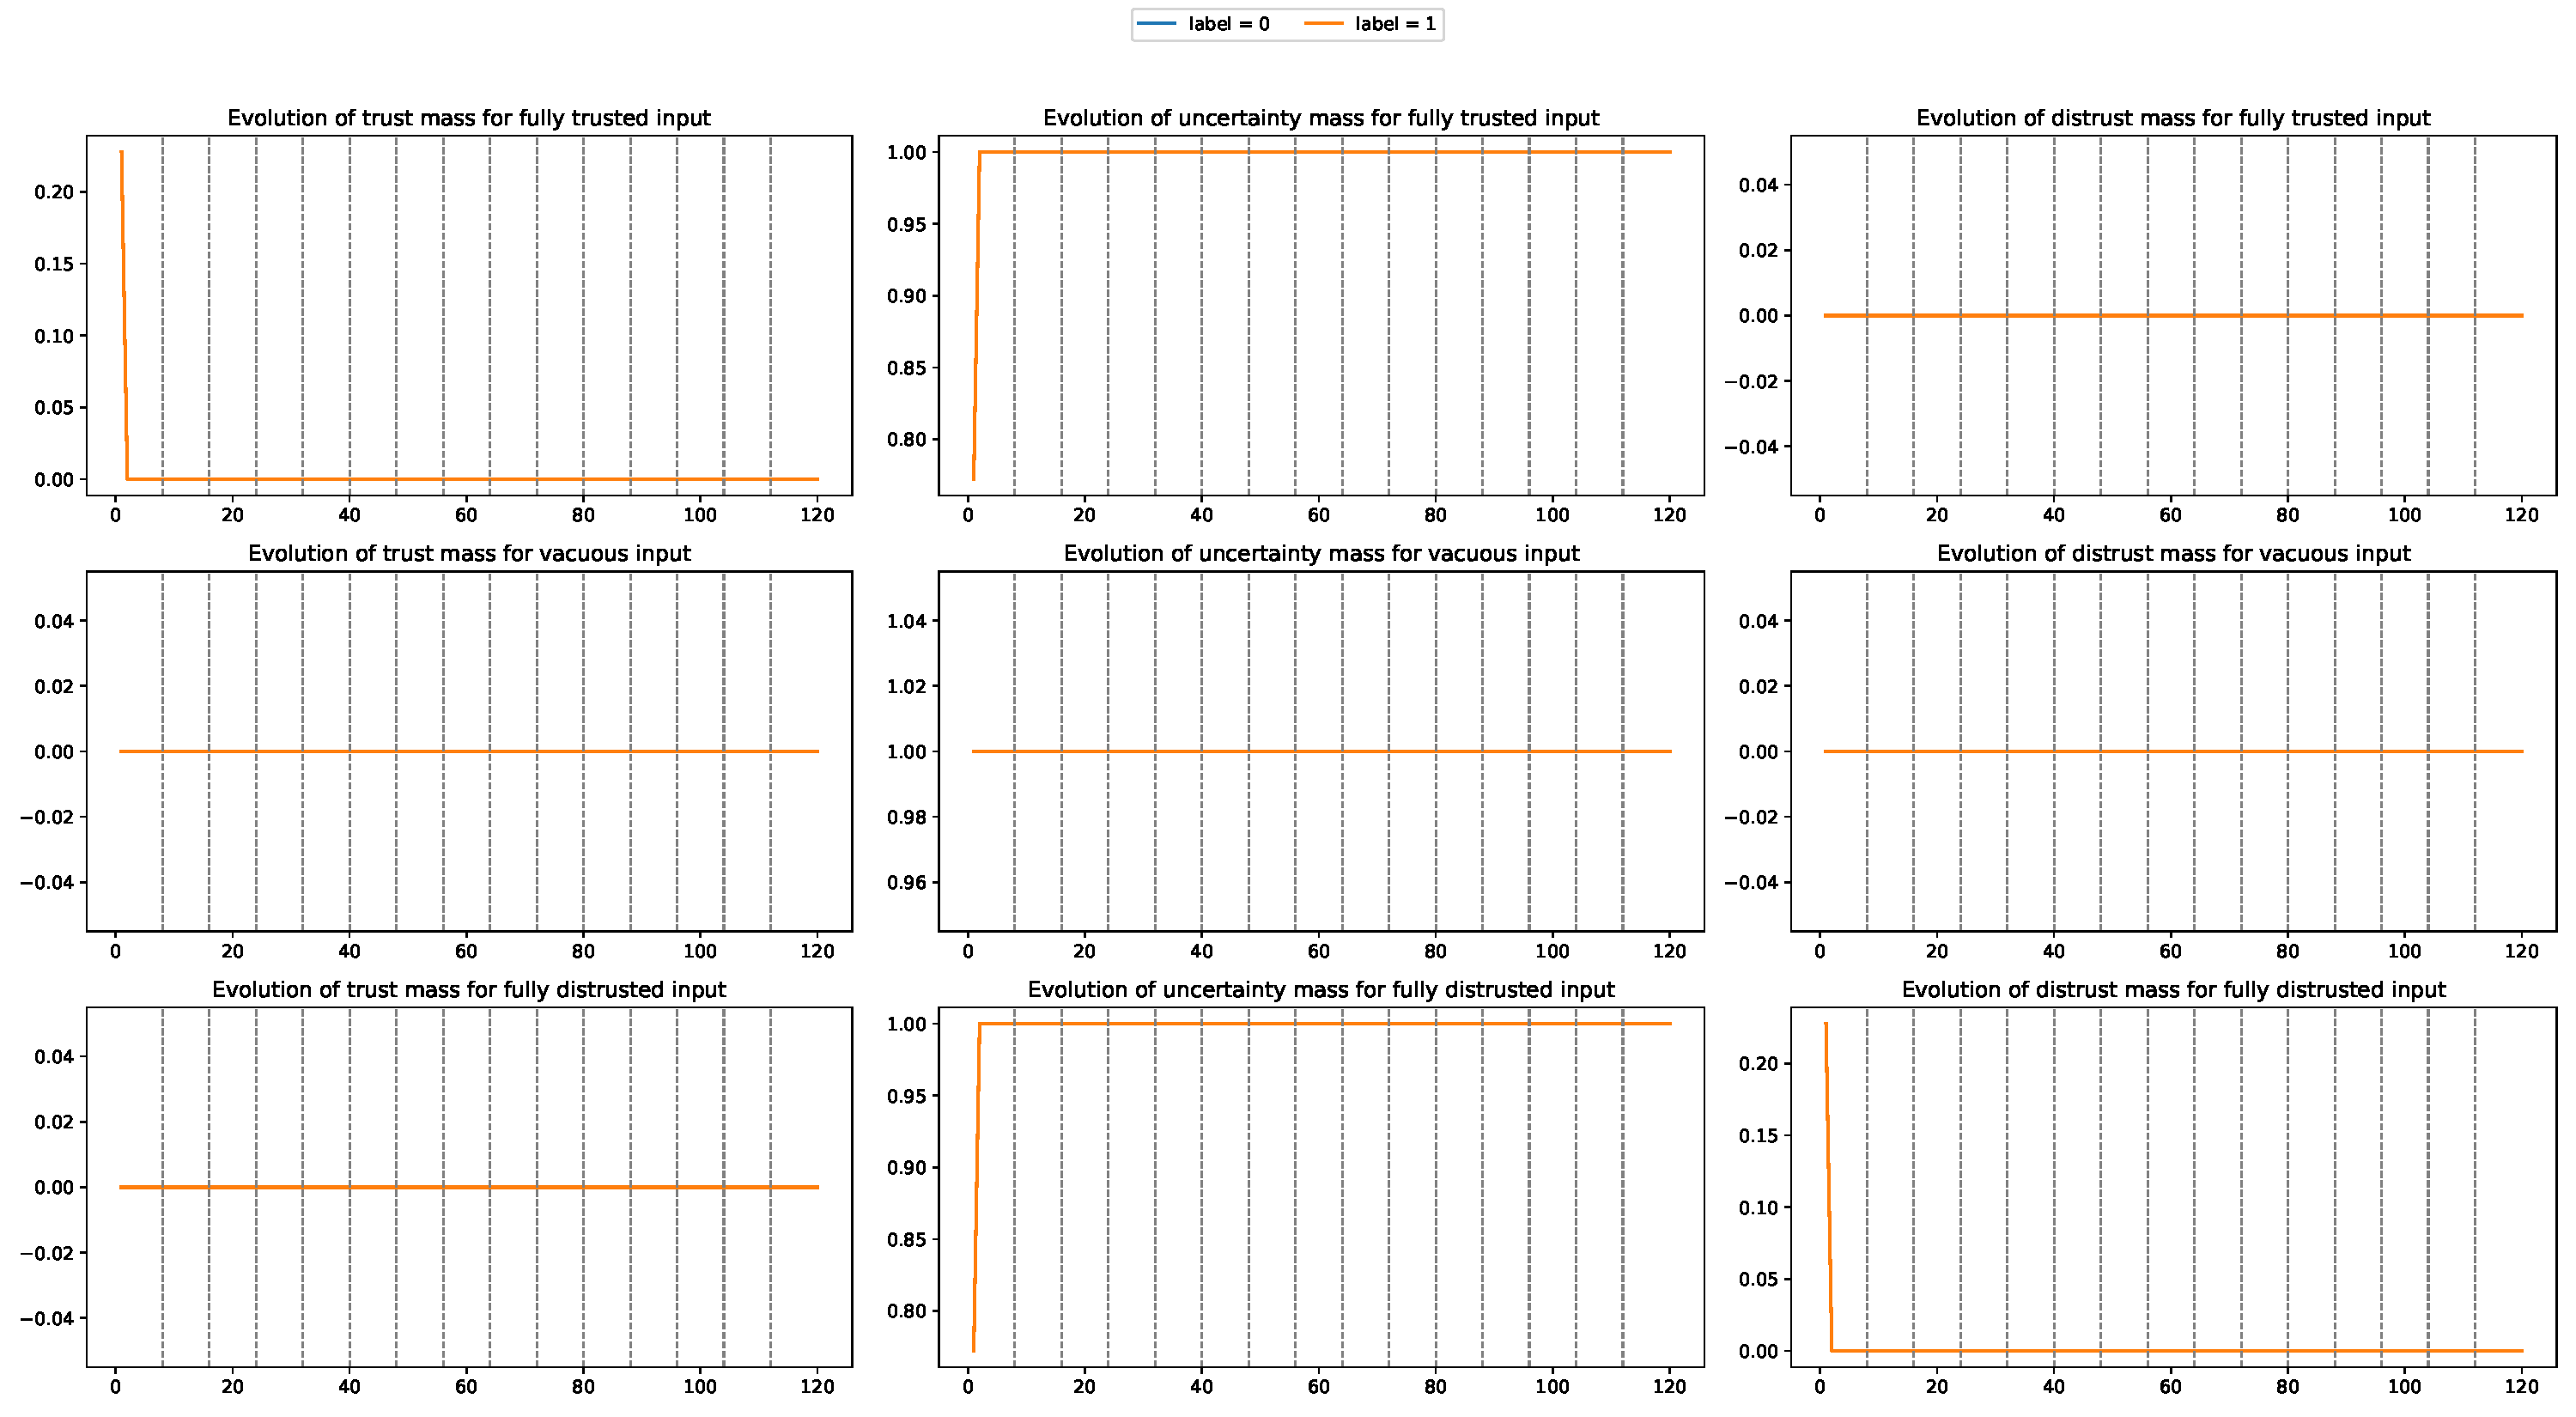
\includegraphics[width=0.8\textwidth]{latex/PTAS_Eval_cancer_16_distrust_distrust_eps_1_PathSize_None__plot_ptas.pdf}
\caption{cancer\_16\_distrust\_distrust, $\varepsilon$=1}
\end{figure}

\subsubsection{distrust -- trust}

\begin{figure}[htbp]
\centering
  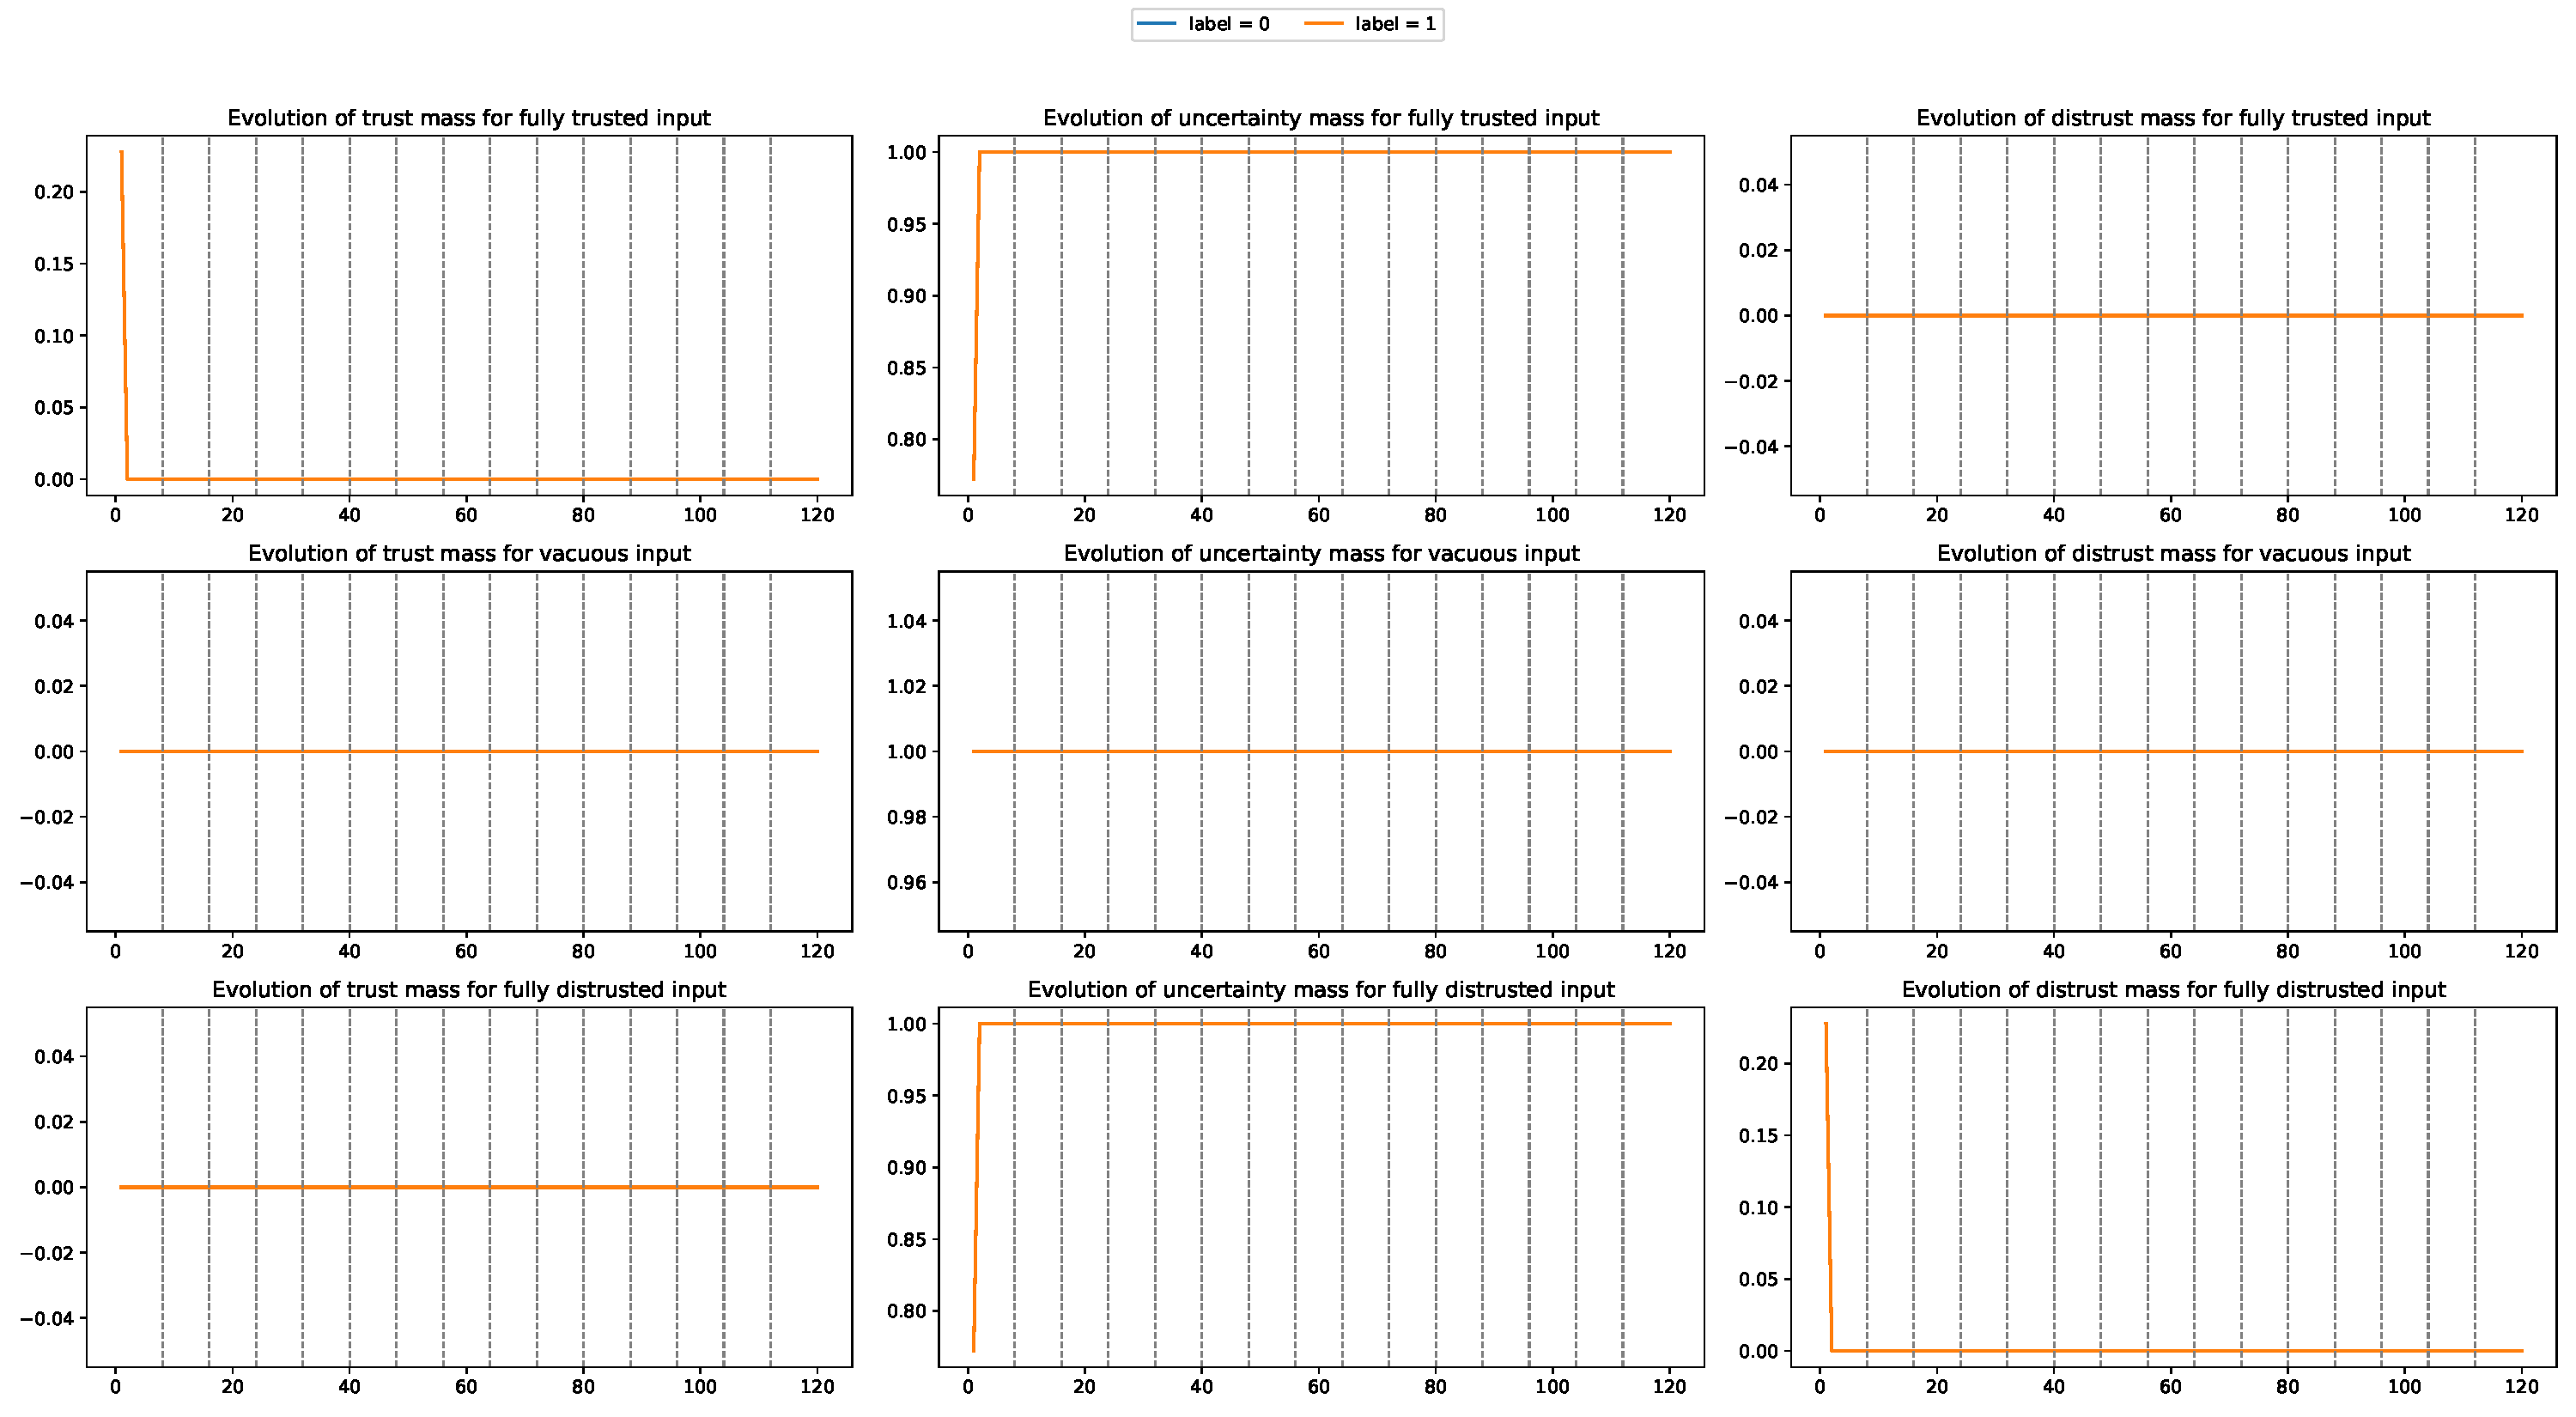
\includegraphics[width=0.8\textwidth]{latex/PTAS_Eval_cancer_16_distrust_trust_eps_0.001_PathSize_None__plot_ptas.pdf}
\caption{cancer\_16\_distrust\_trust, $\varepsilon$=0.001}
\end{figure}

\begin{figure}[htbp]
\centering
  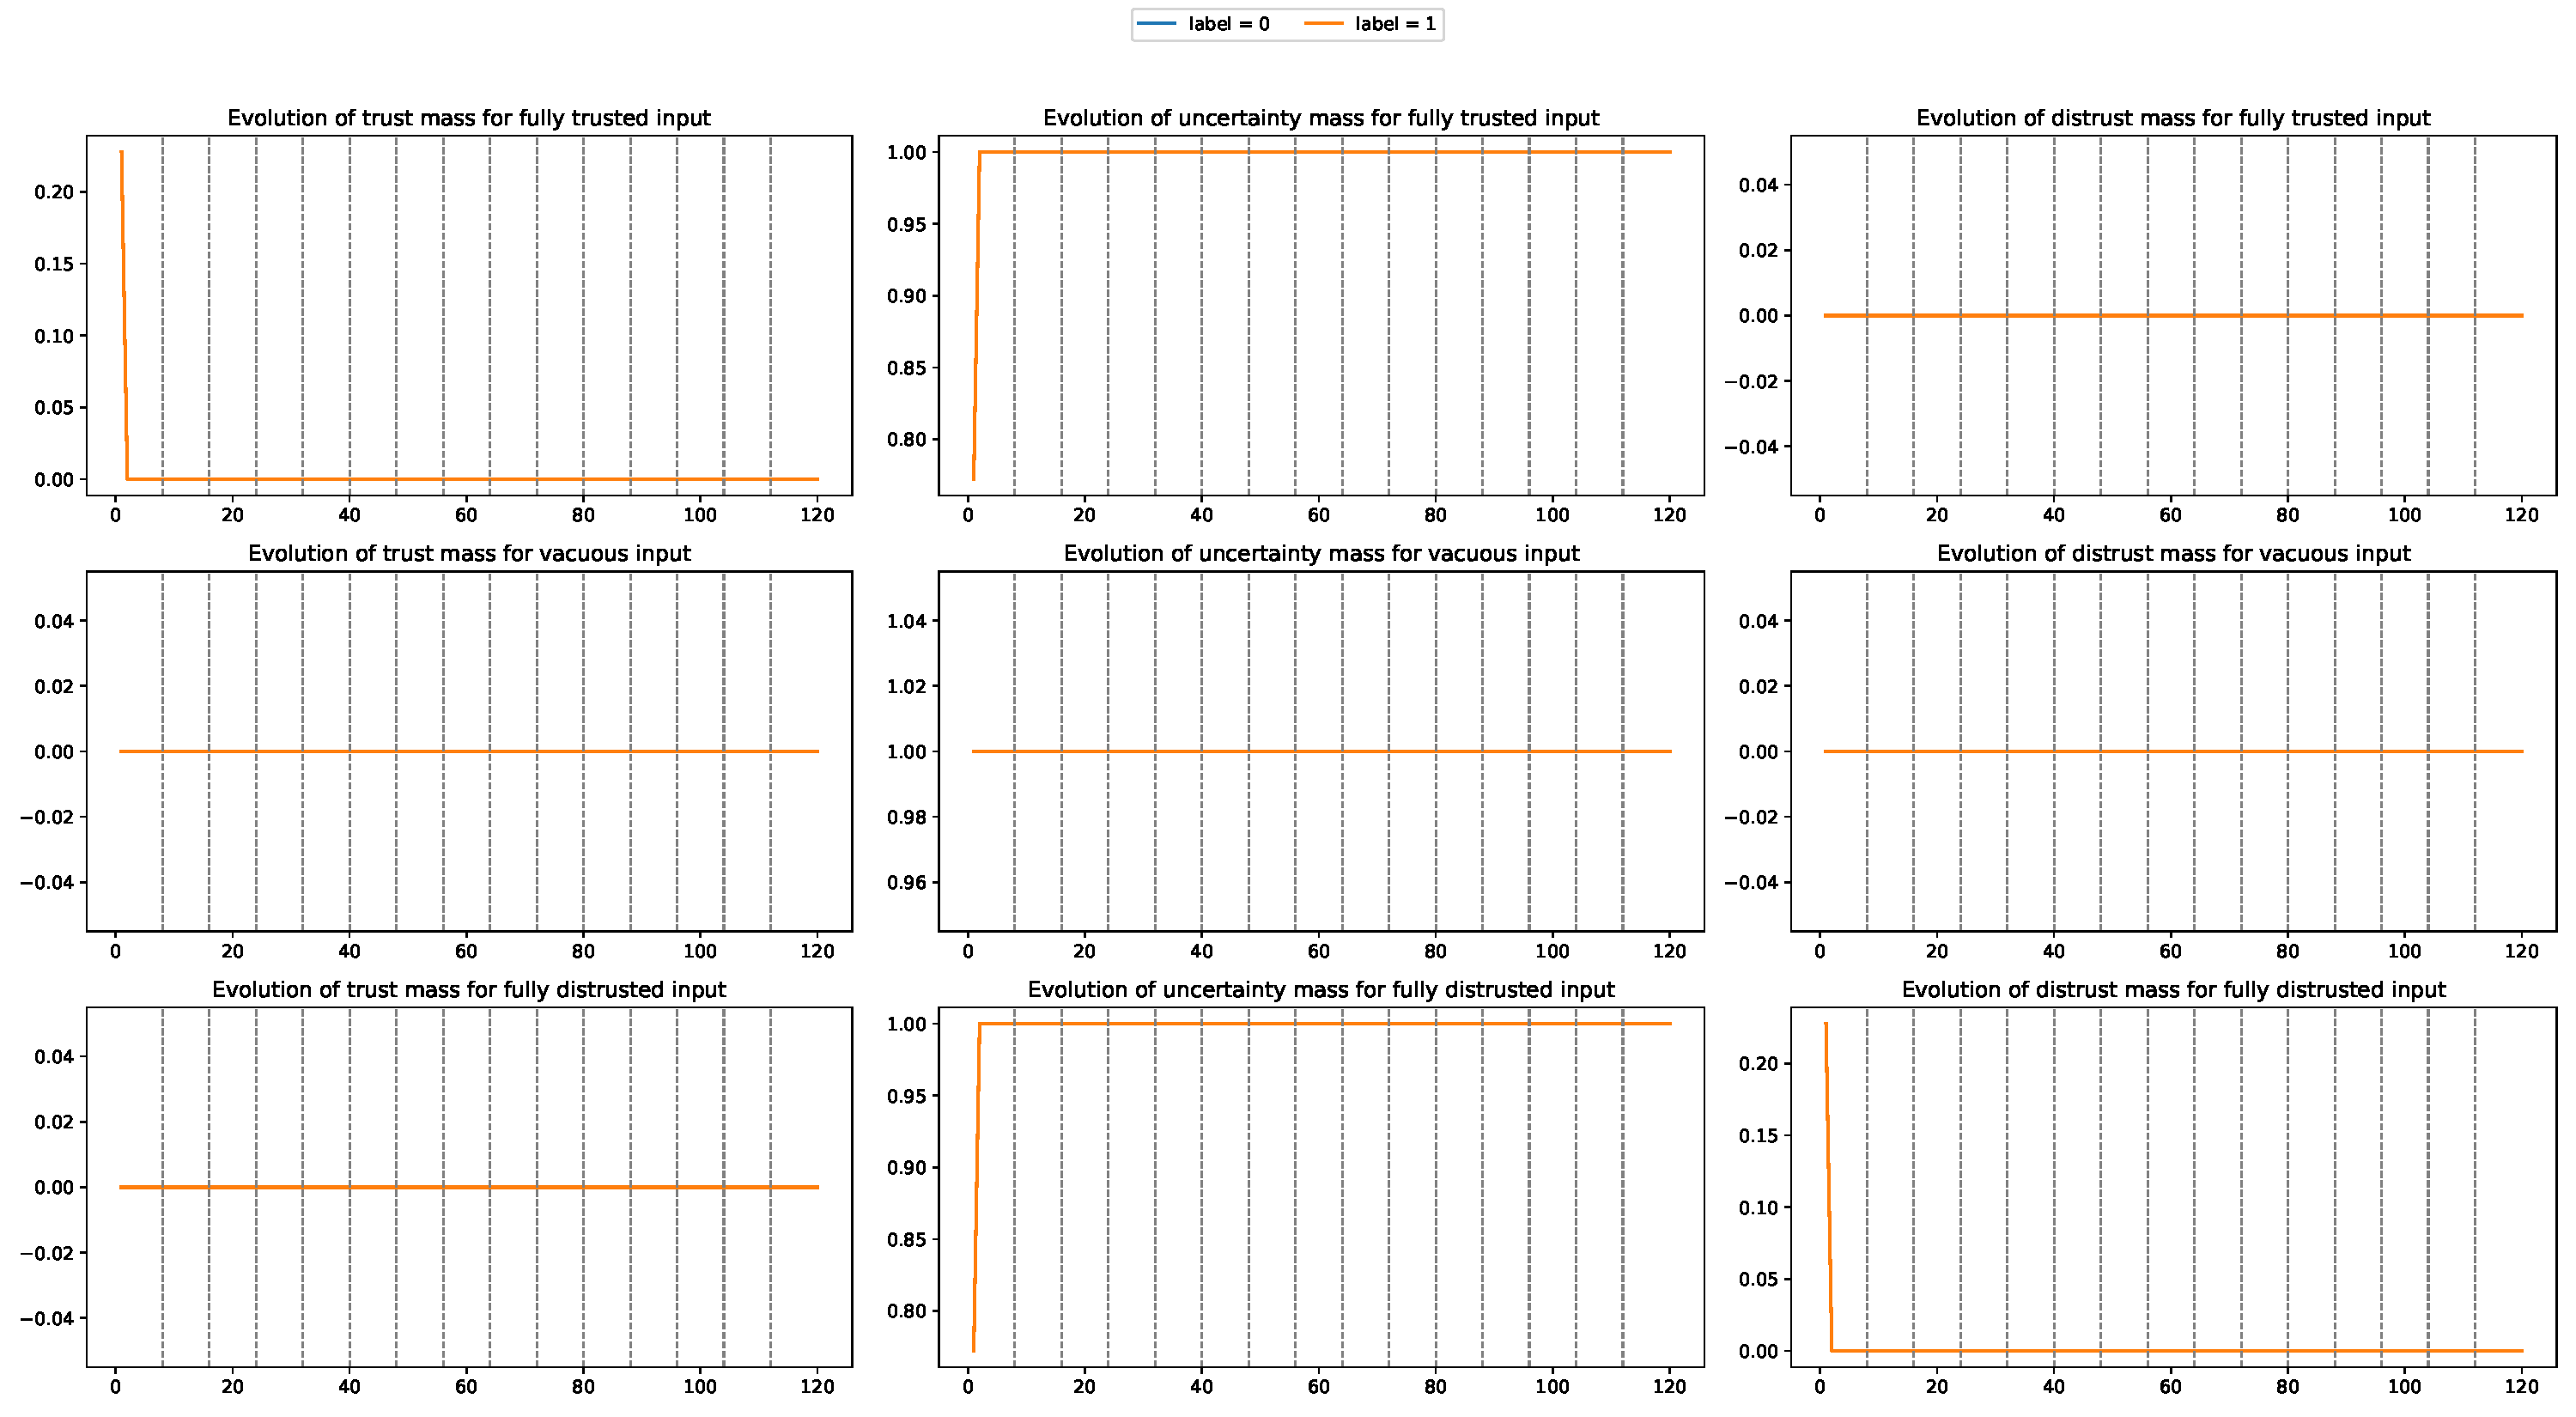
\includegraphics[width=0.8\textwidth]{latex/PTAS_Eval_cancer_16_distrust_trust_eps_0.01_PathSize_None__plot_ptas.pdf}
\caption{cancer\_16\_distrust\_trust, $\varepsilon$=0.01}
\end{figure}

\begin{figure}[htbp]
\centering
  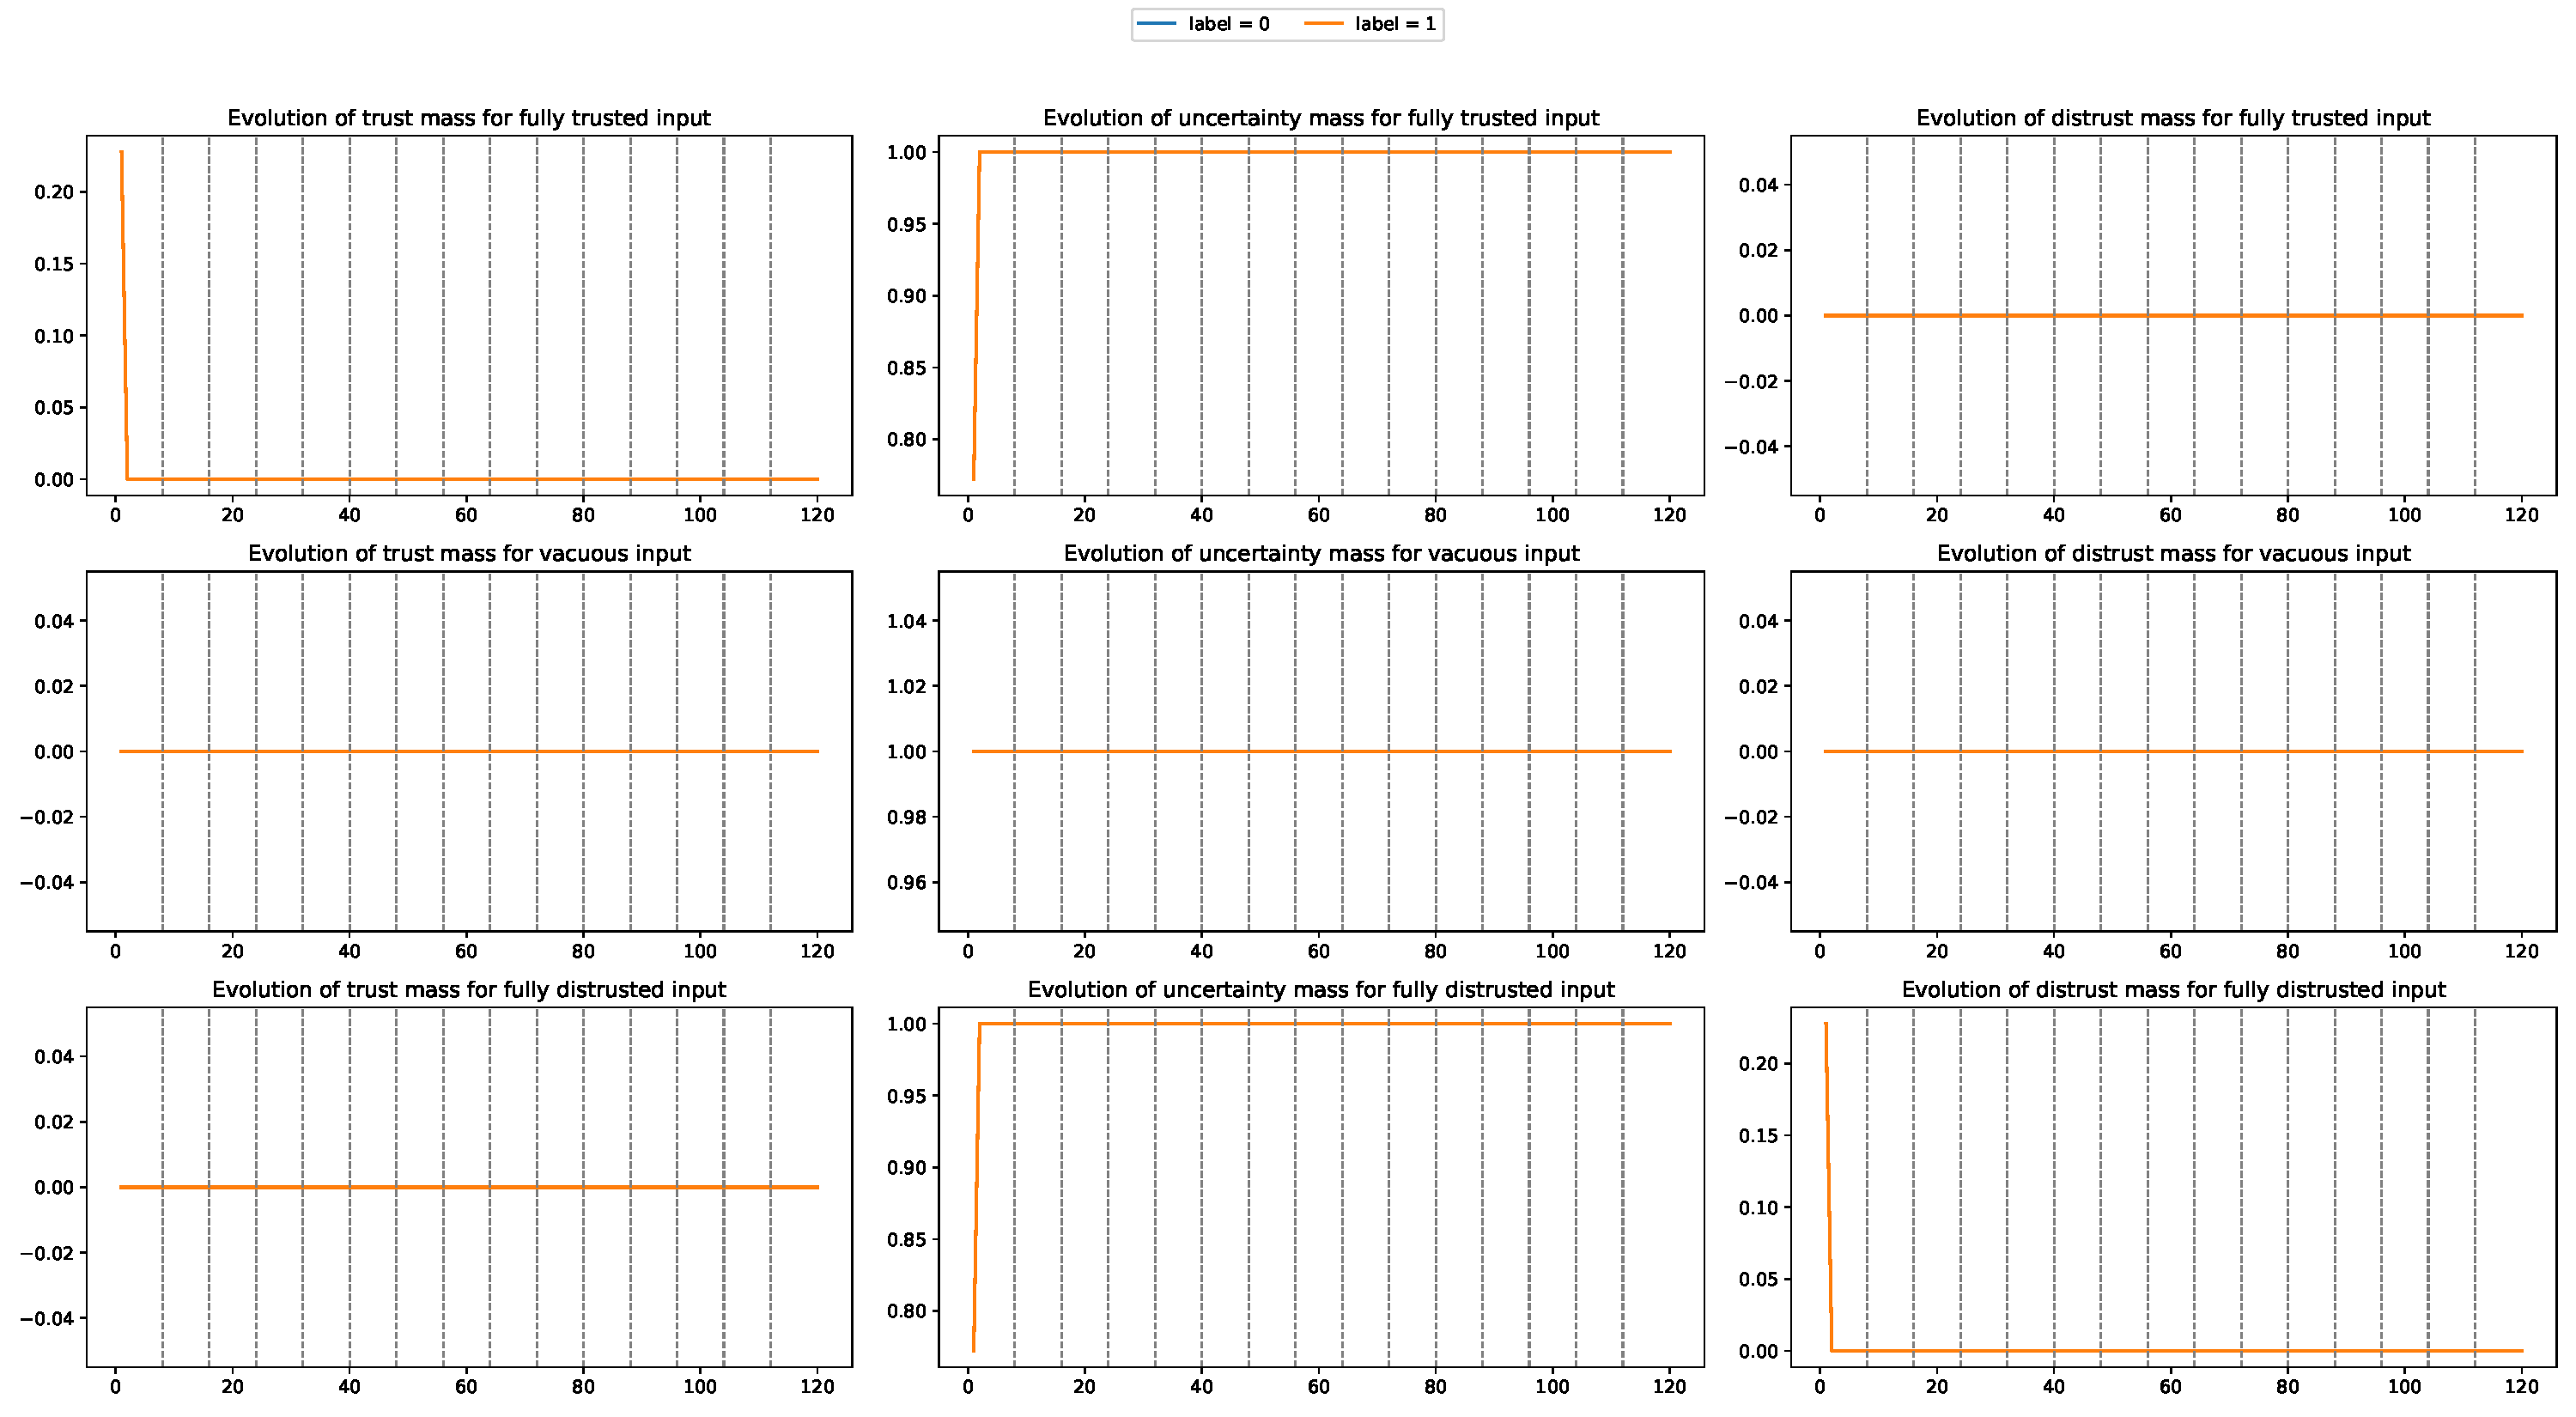
\includegraphics[width=0.8\textwidth]{latex/PTAS_Eval_cancer_16_distrust_trust_eps_0.1_PathSize_None__plot_ptas.pdf}
\caption{cancer\_16\_distrust\_trust, $\varepsilon$=0.1}
\end{figure}

\begin{figure}[htbp]
\centering
  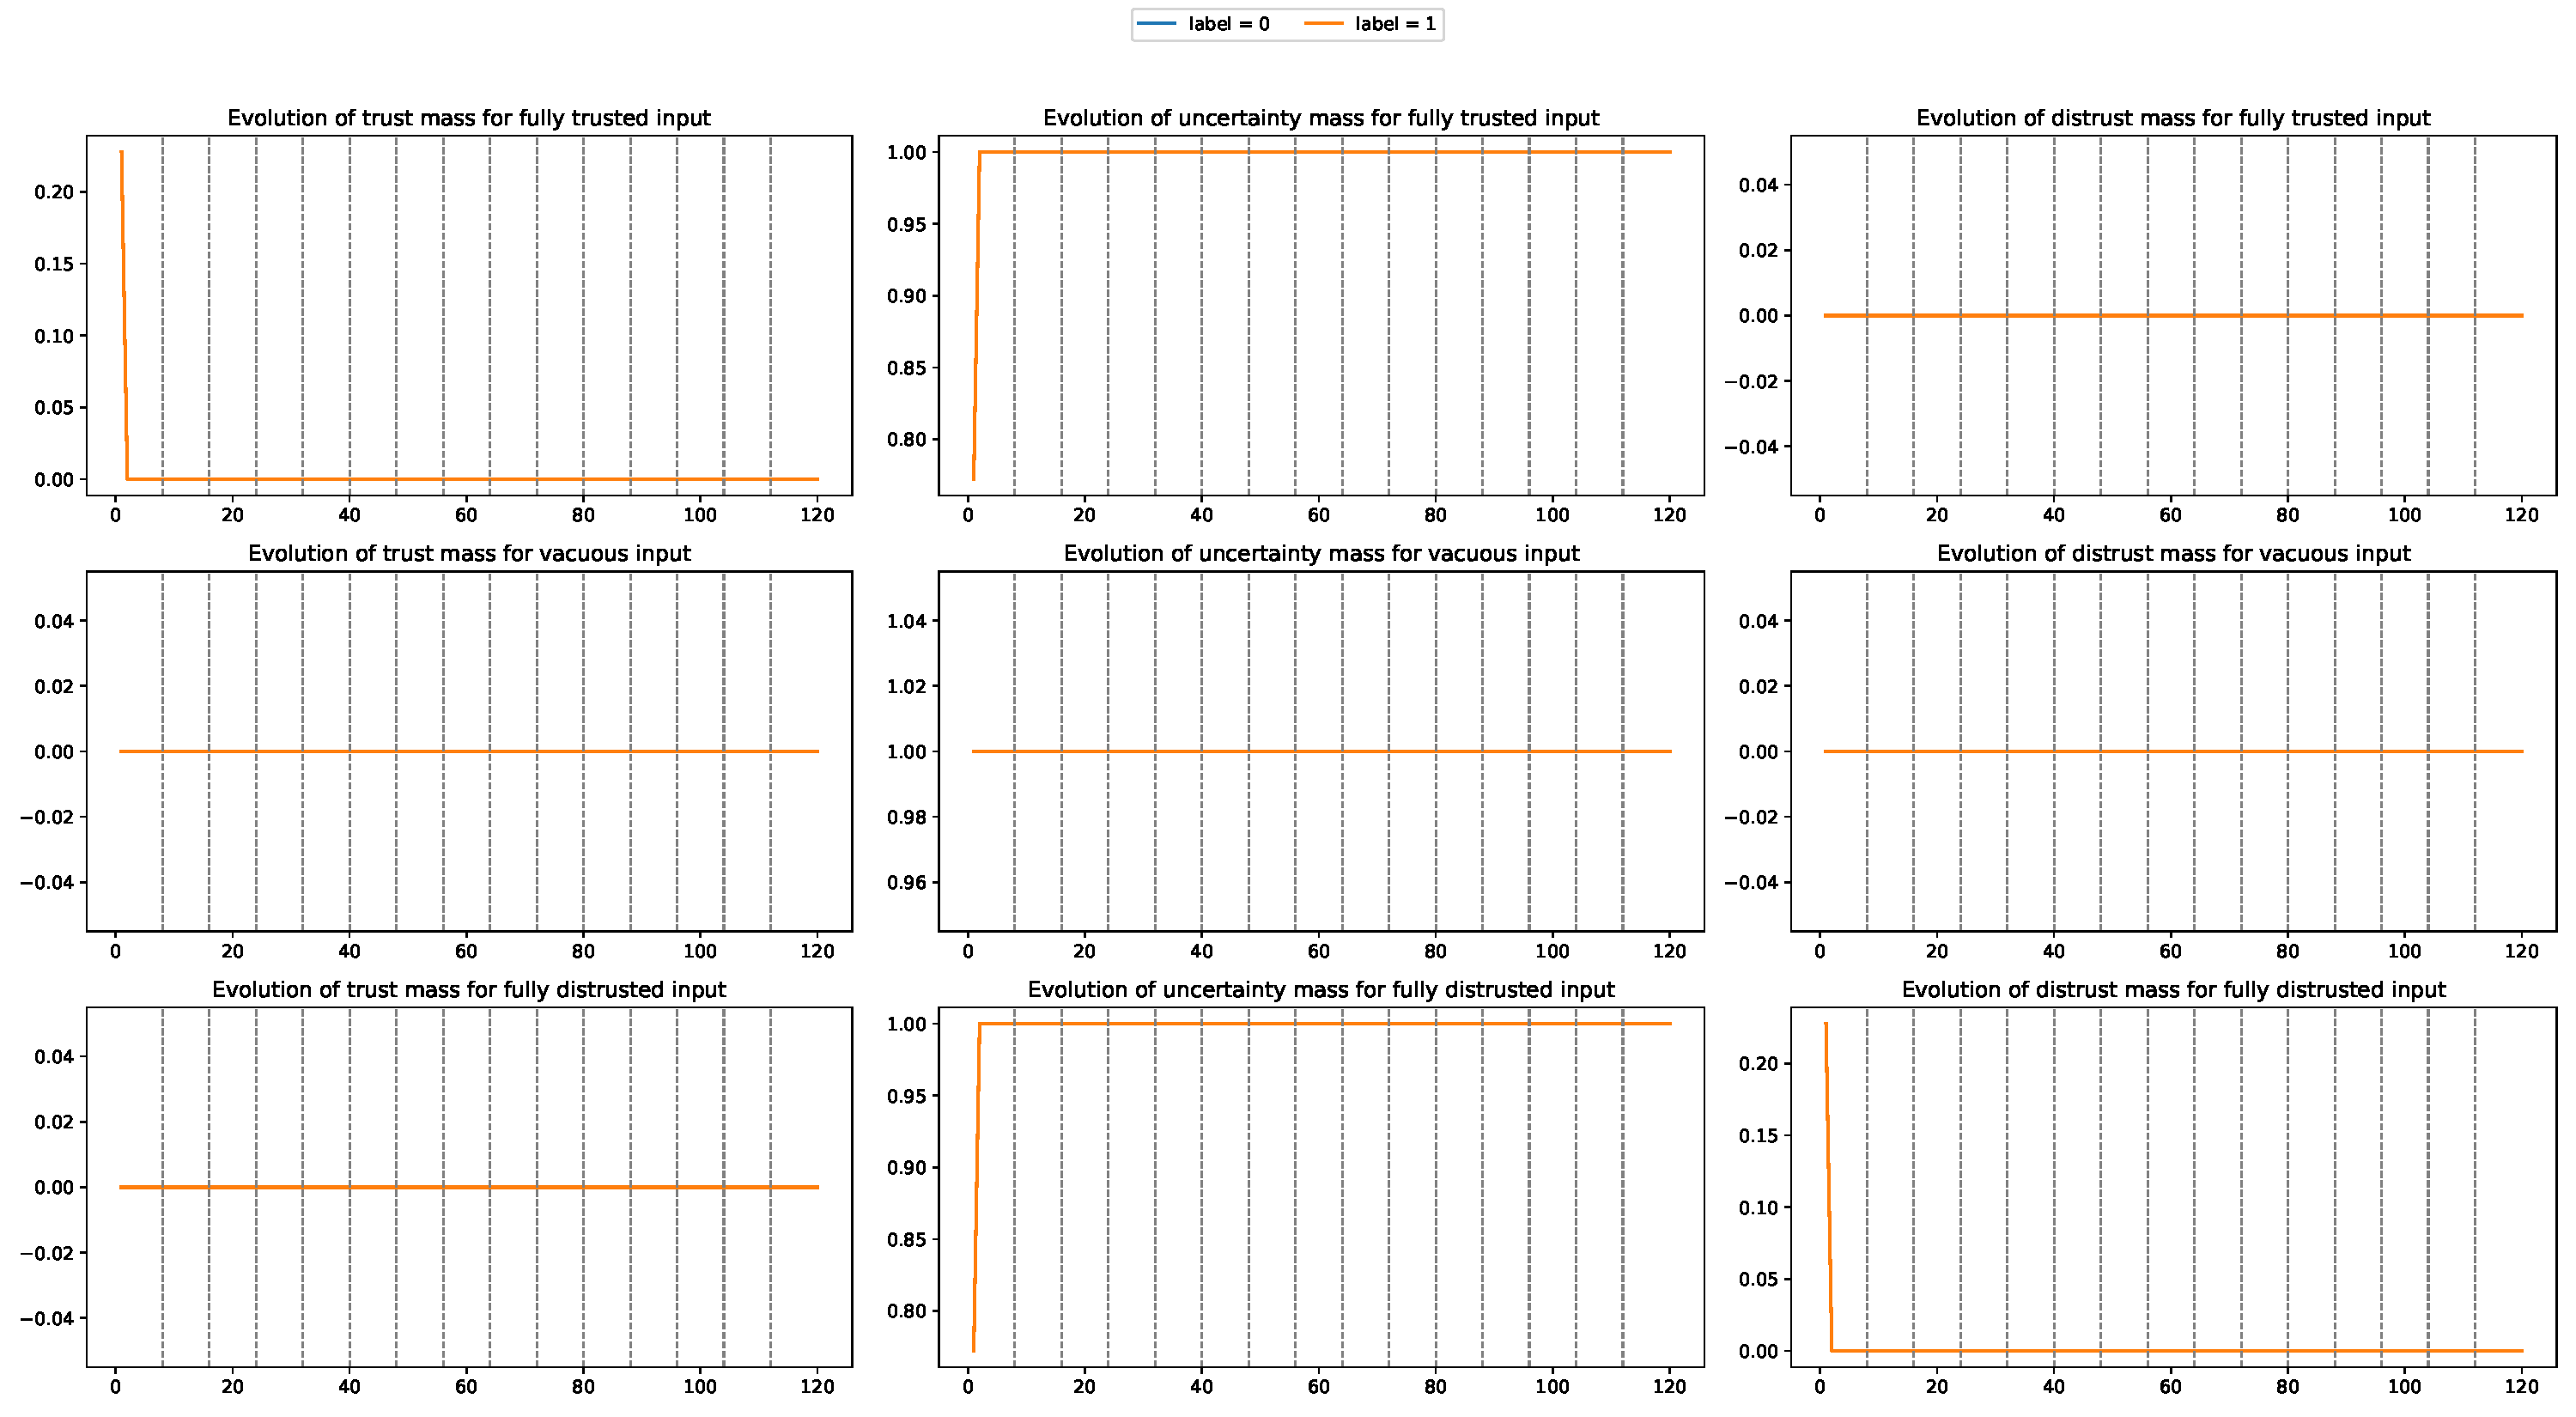
\includegraphics[width=0.8\textwidth]{latex/PTAS_Eval_cancer_16_distrust_trust_eps_1_PathSize_None__plot_ptas.pdf}
\caption{cancer\_16\_distrust\_trust, $\varepsilon$=1}
\end{figure}

\subsubsection{distrust -- vacuous}

\begin{figure}[htbp]
\centering
  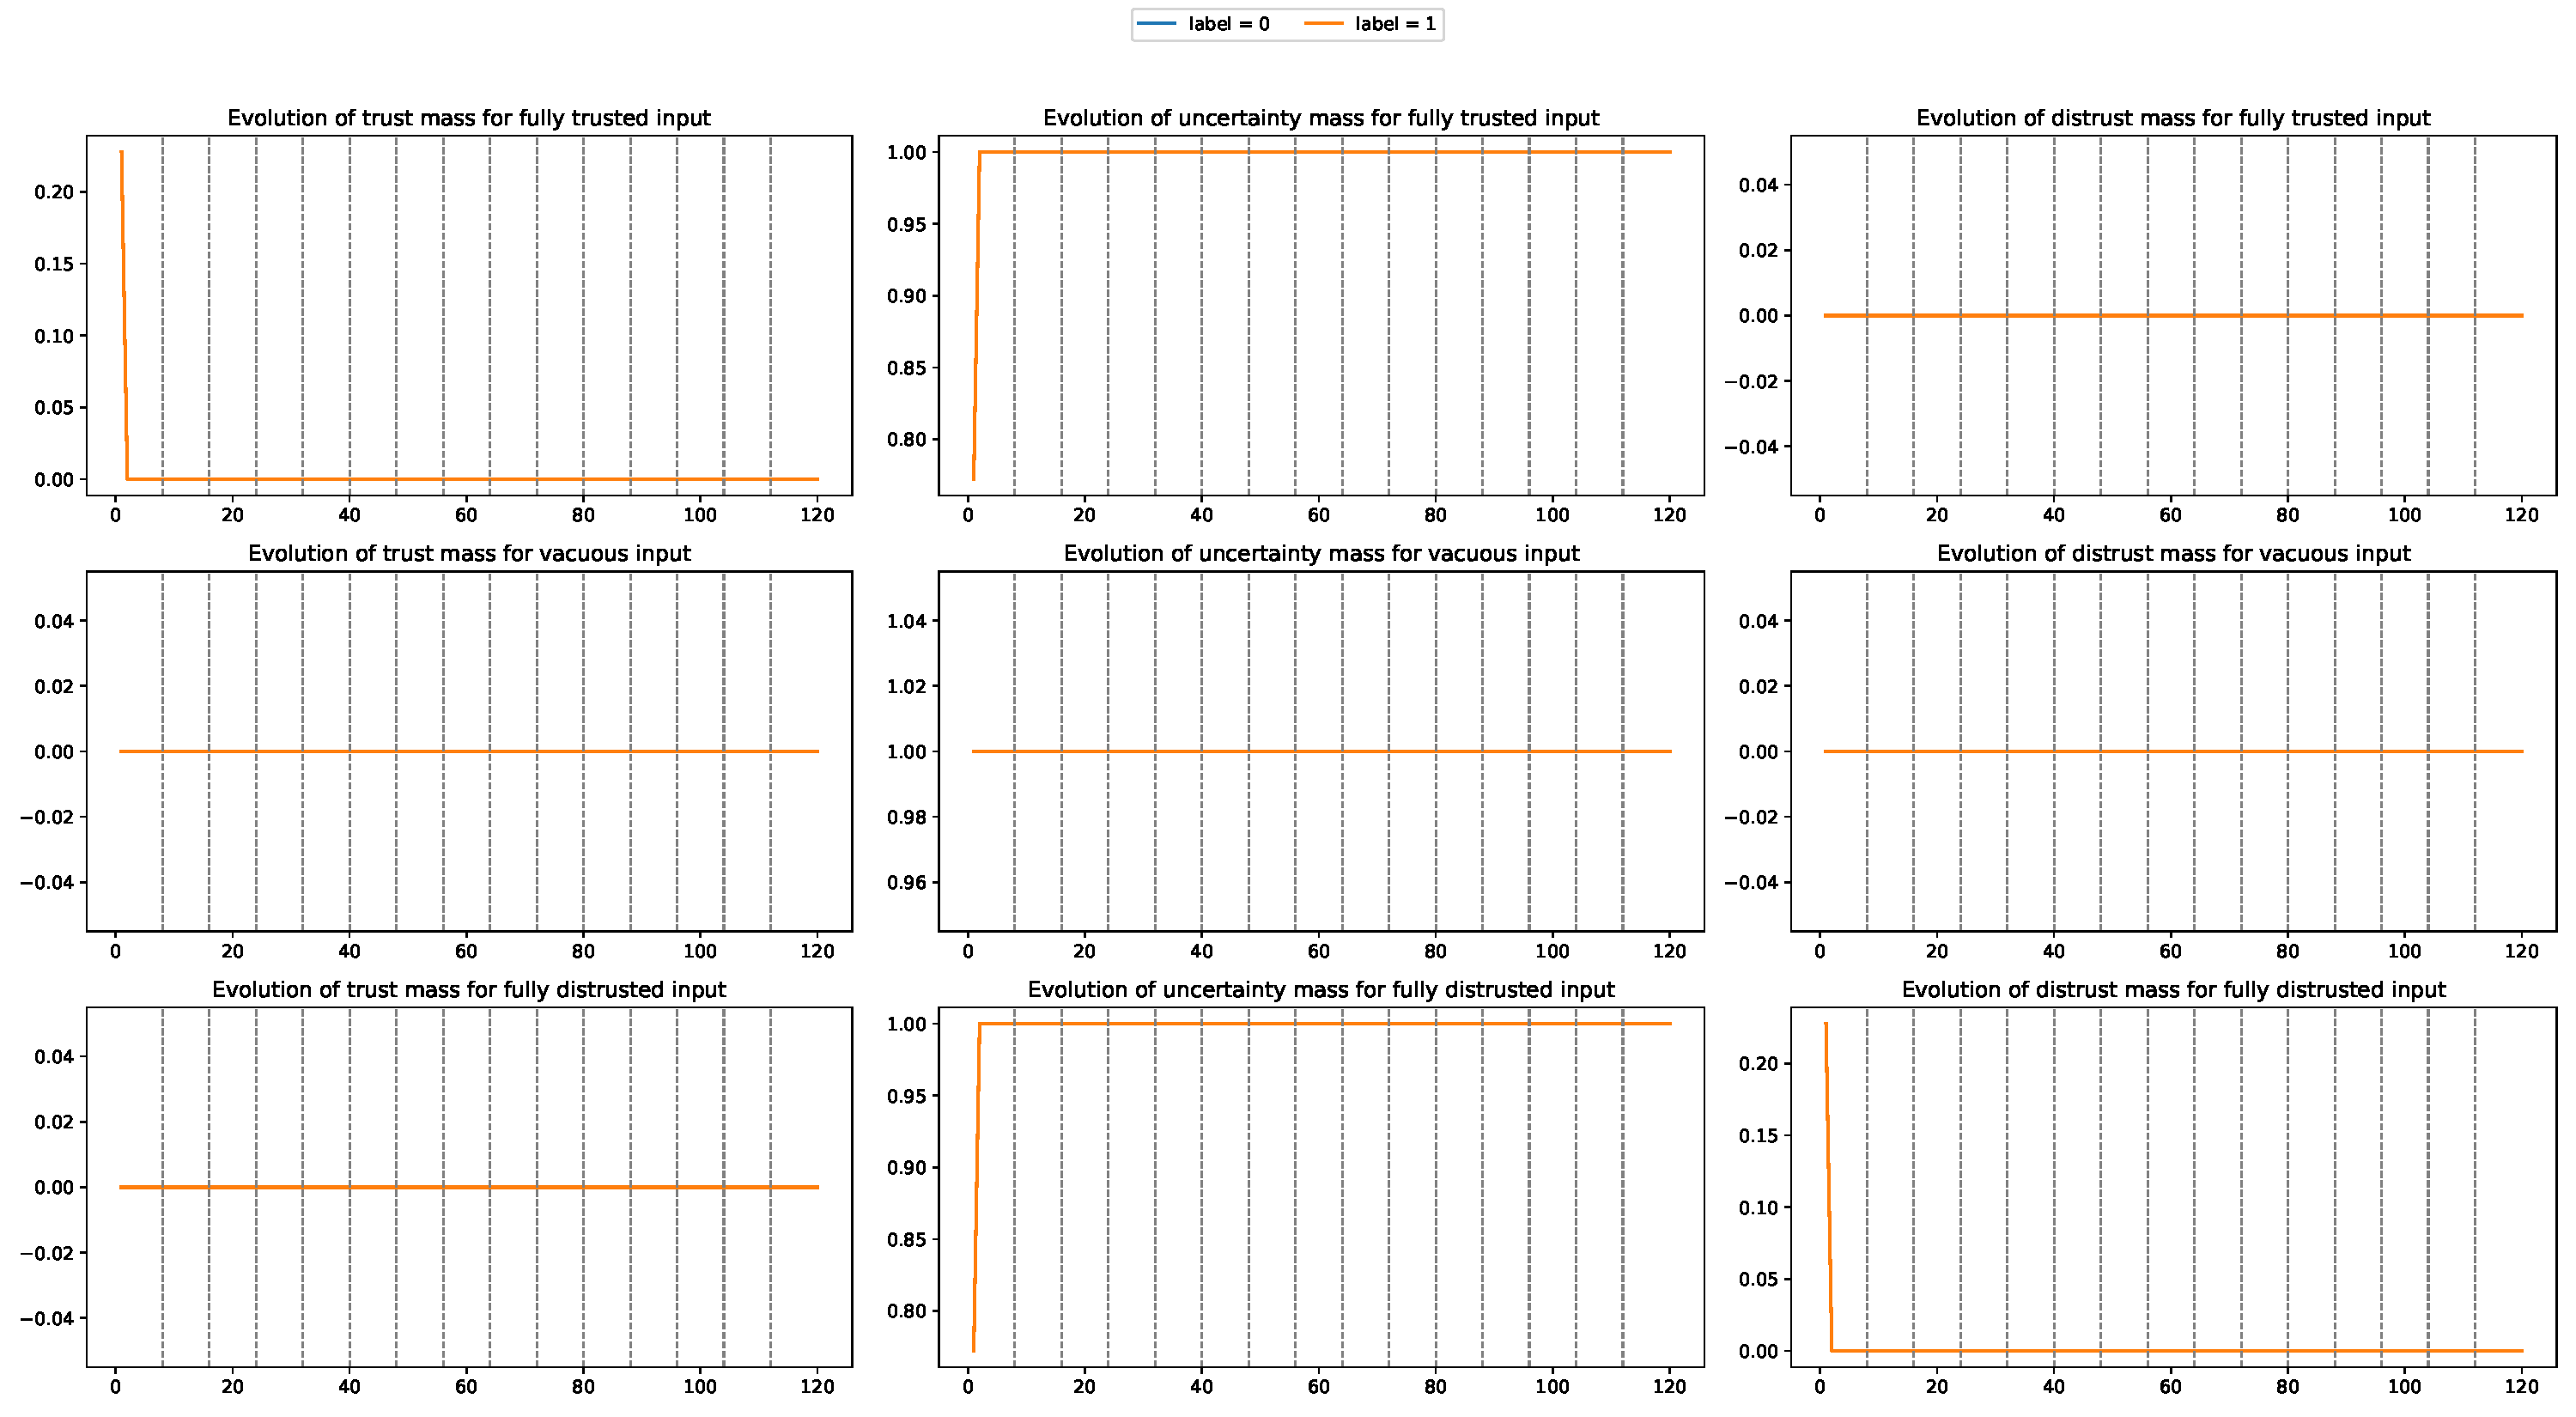
\includegraphics[width=0.8\textwidth]{latex/PTAS_Eval_cancer_16_distrust_vacuous_eps_0.001_PathSize_None__plot_ptas.pdf}
\caption{cancer\_16\_distrust\_vacuous, $\varepsilon$=0.001}
\end{figure}

\begin{figure}[htbp]
\centering
  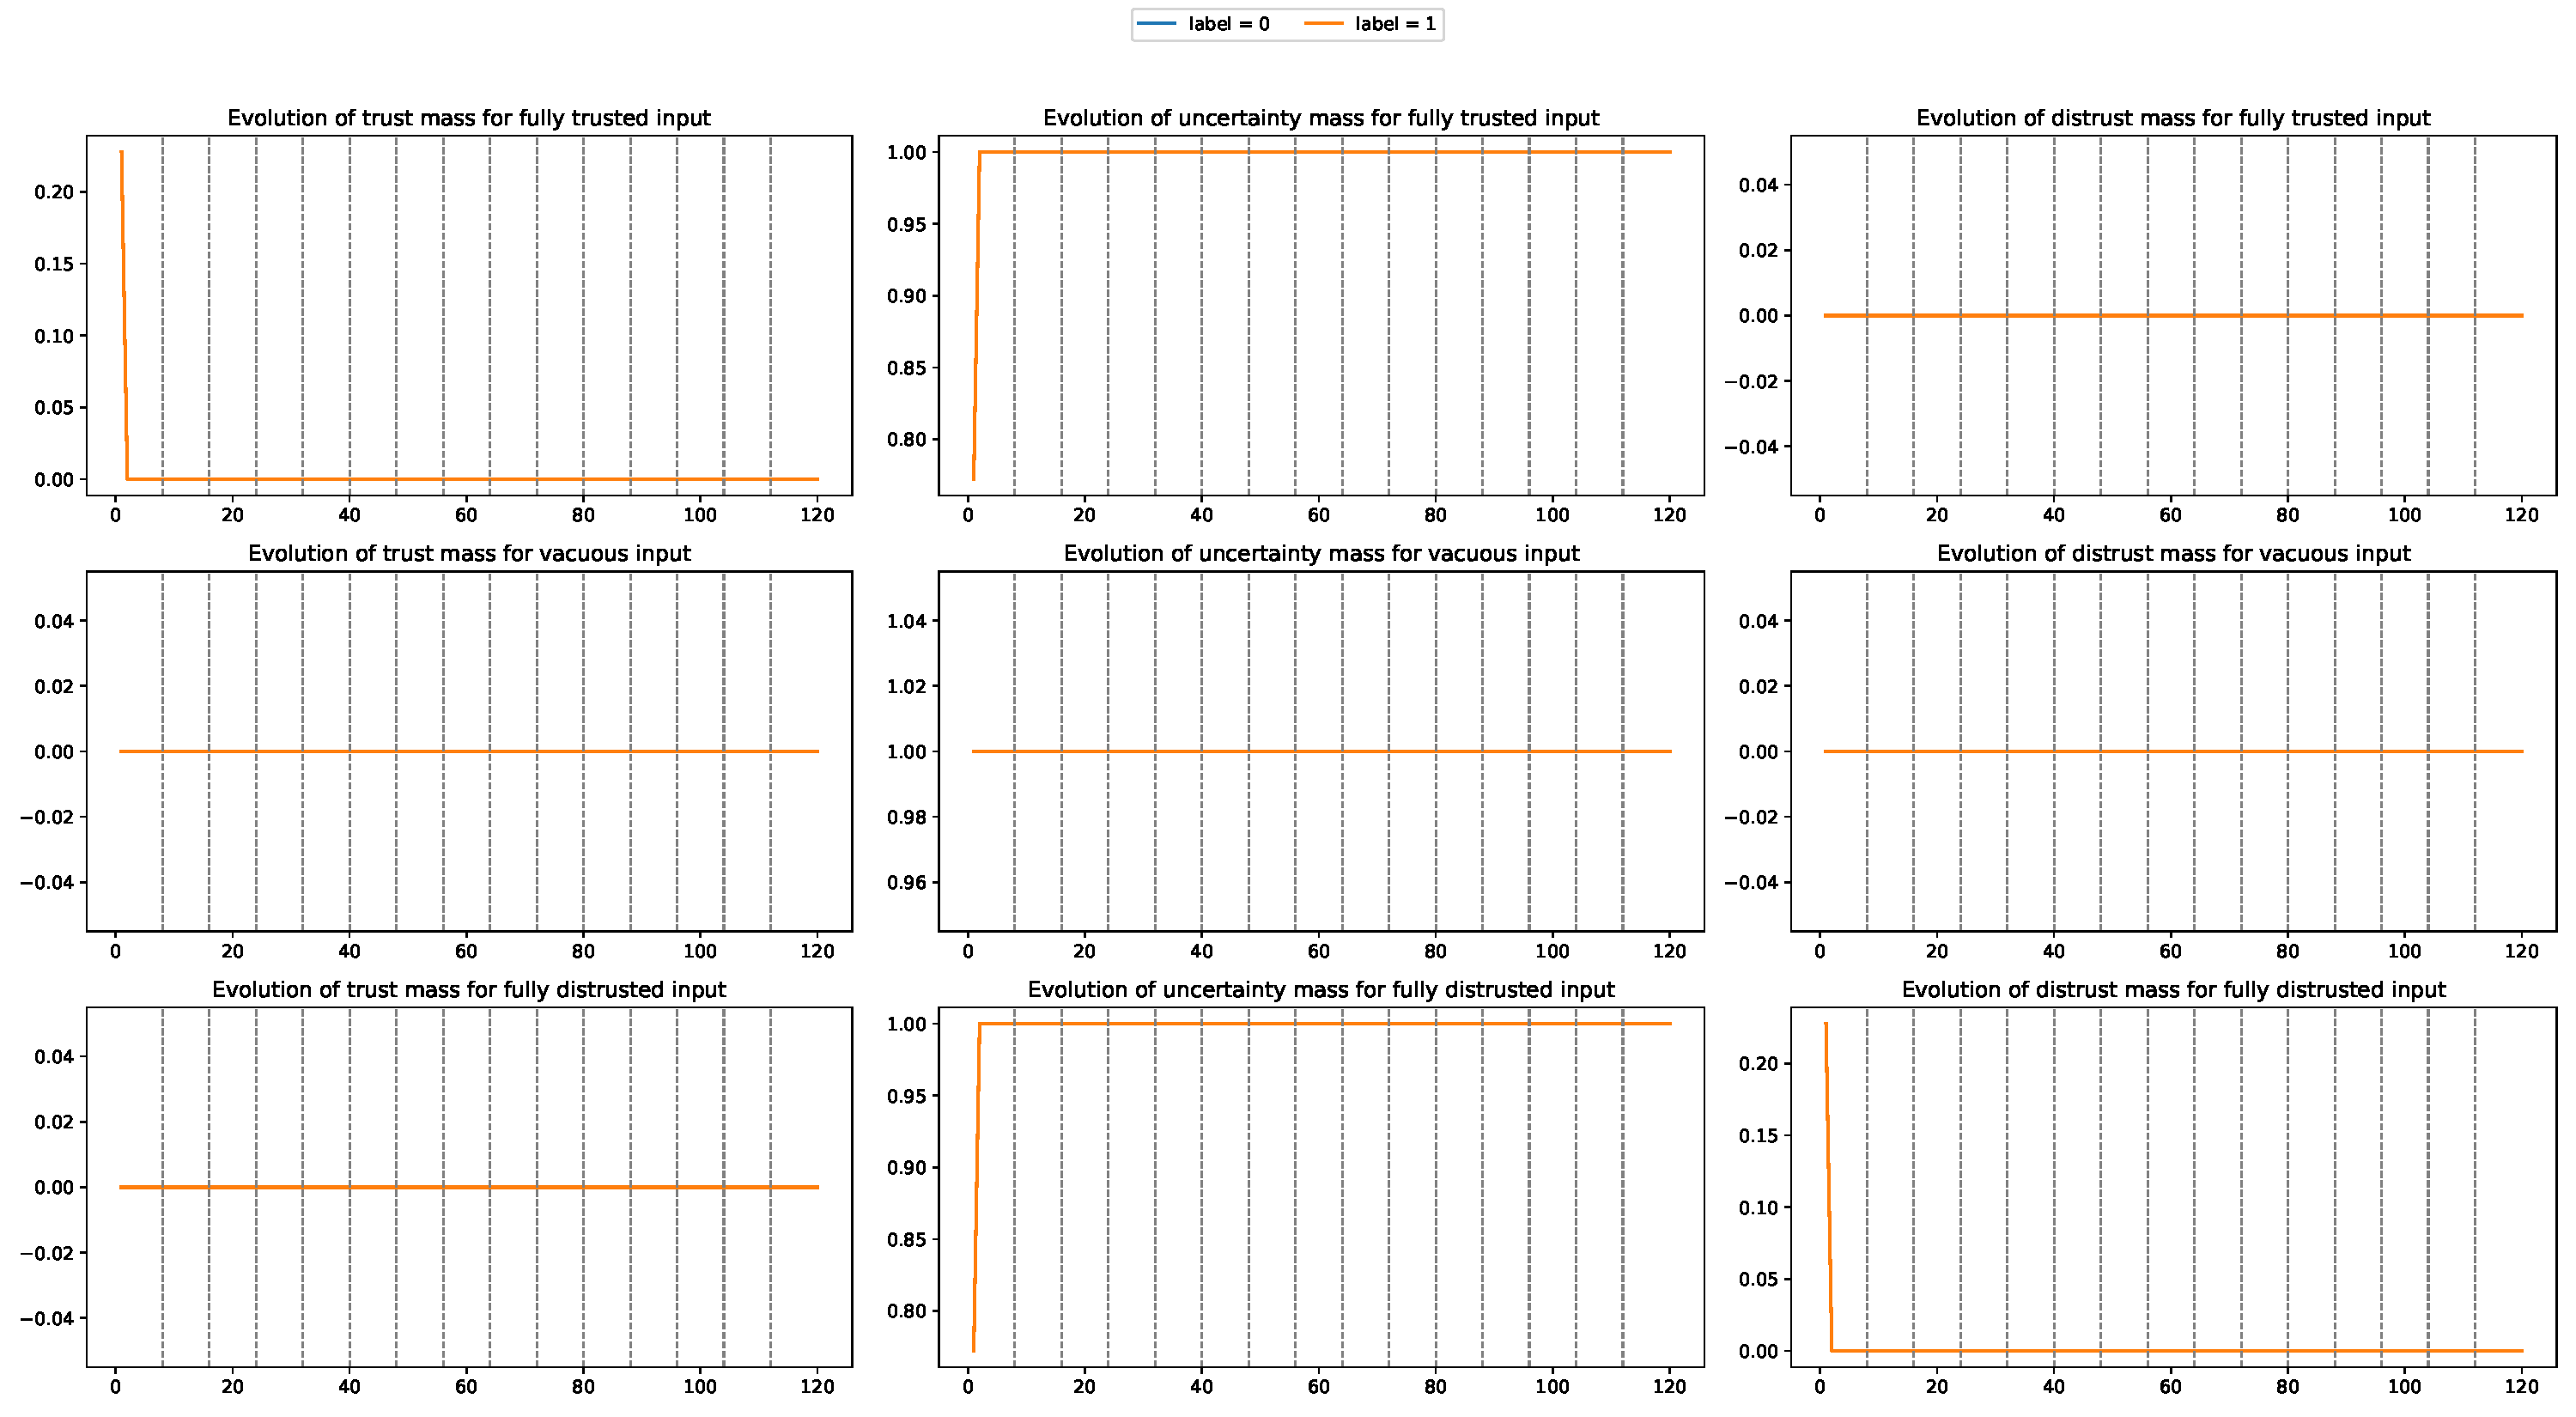
\includegraphics[width=0.8\textwidth]{latex/PTAS_Eval_cancer_16_distrust_vacuous_eps_0.01_PathSize_None__plot_ptas.pdf}
\caption{cancer\_16\_distrust\_vacuous, $\varepsilon$=0.01}
\end{figure}

\begin{figure}[htbp]
\centering
  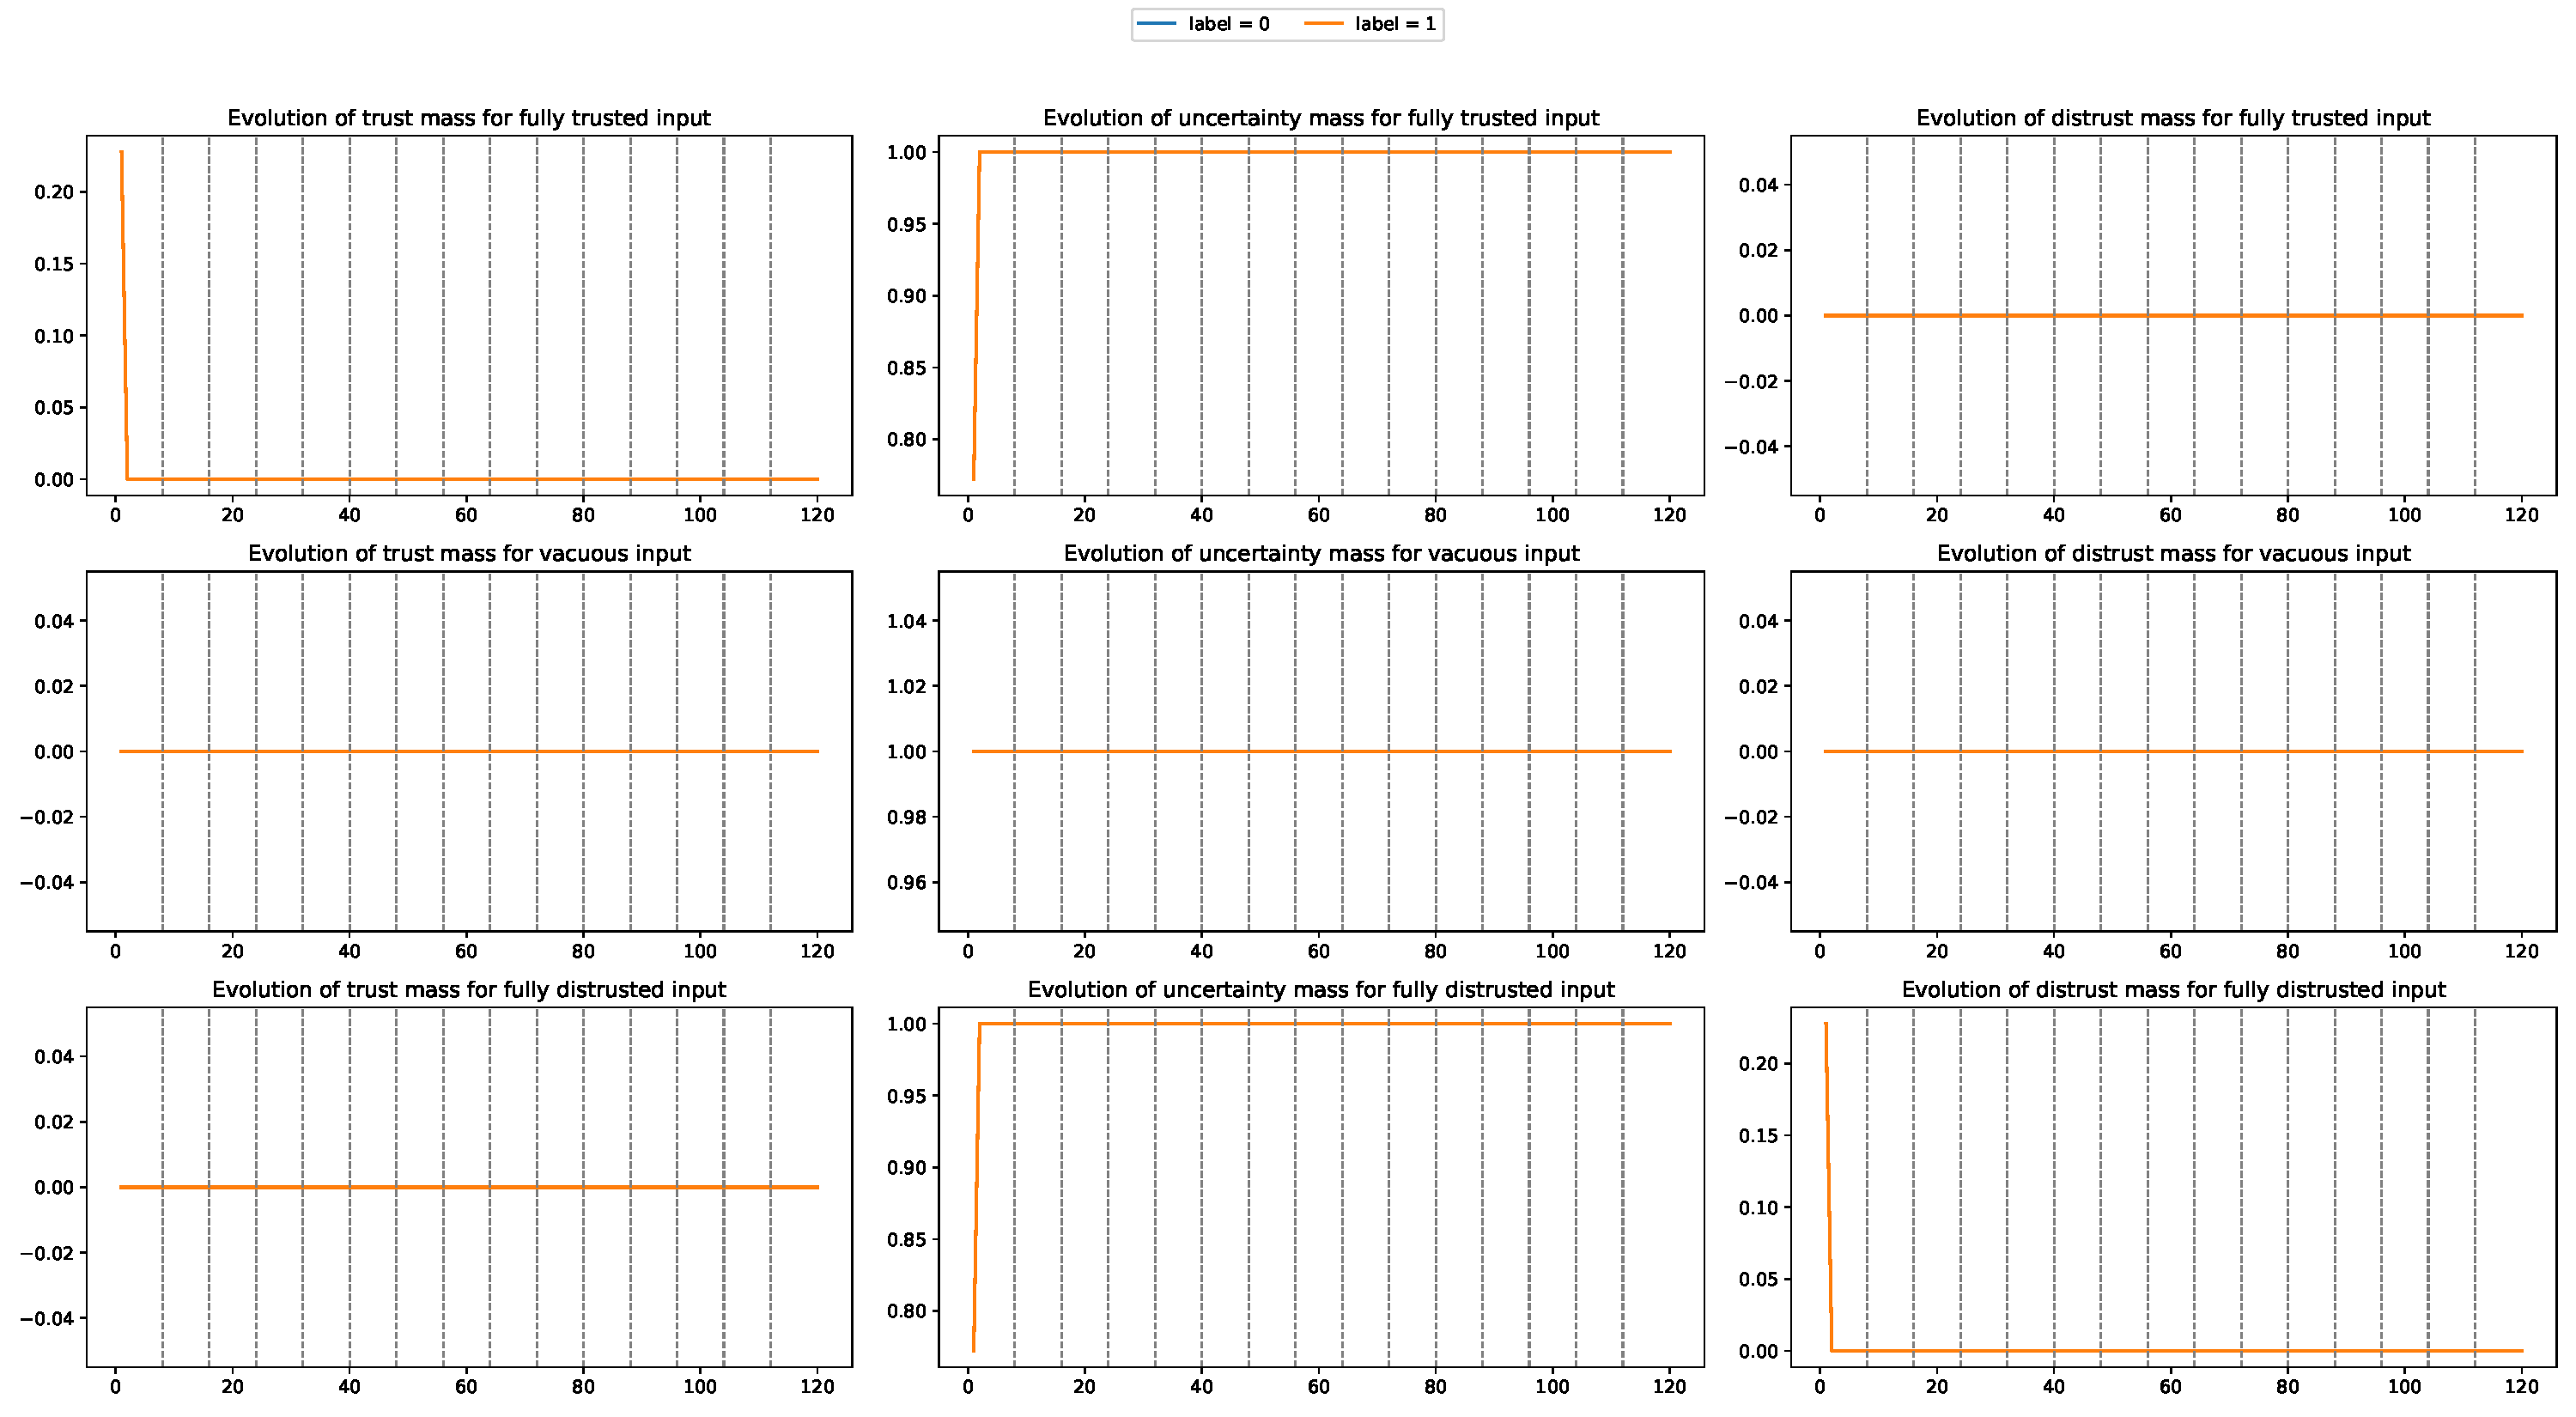
\includegraphics[width=0.8\textwidth]{latex/PTAS_Eval_cancer_16_distrust_vacuous_eps_0.1_PathSize_None__plot_ptas.pdf}
\caption{cancer\_16\_distrust\_vacuous, $\varepsilon$=0.1}
\end{figure}

\begin{figure}[htbp]
\centering
  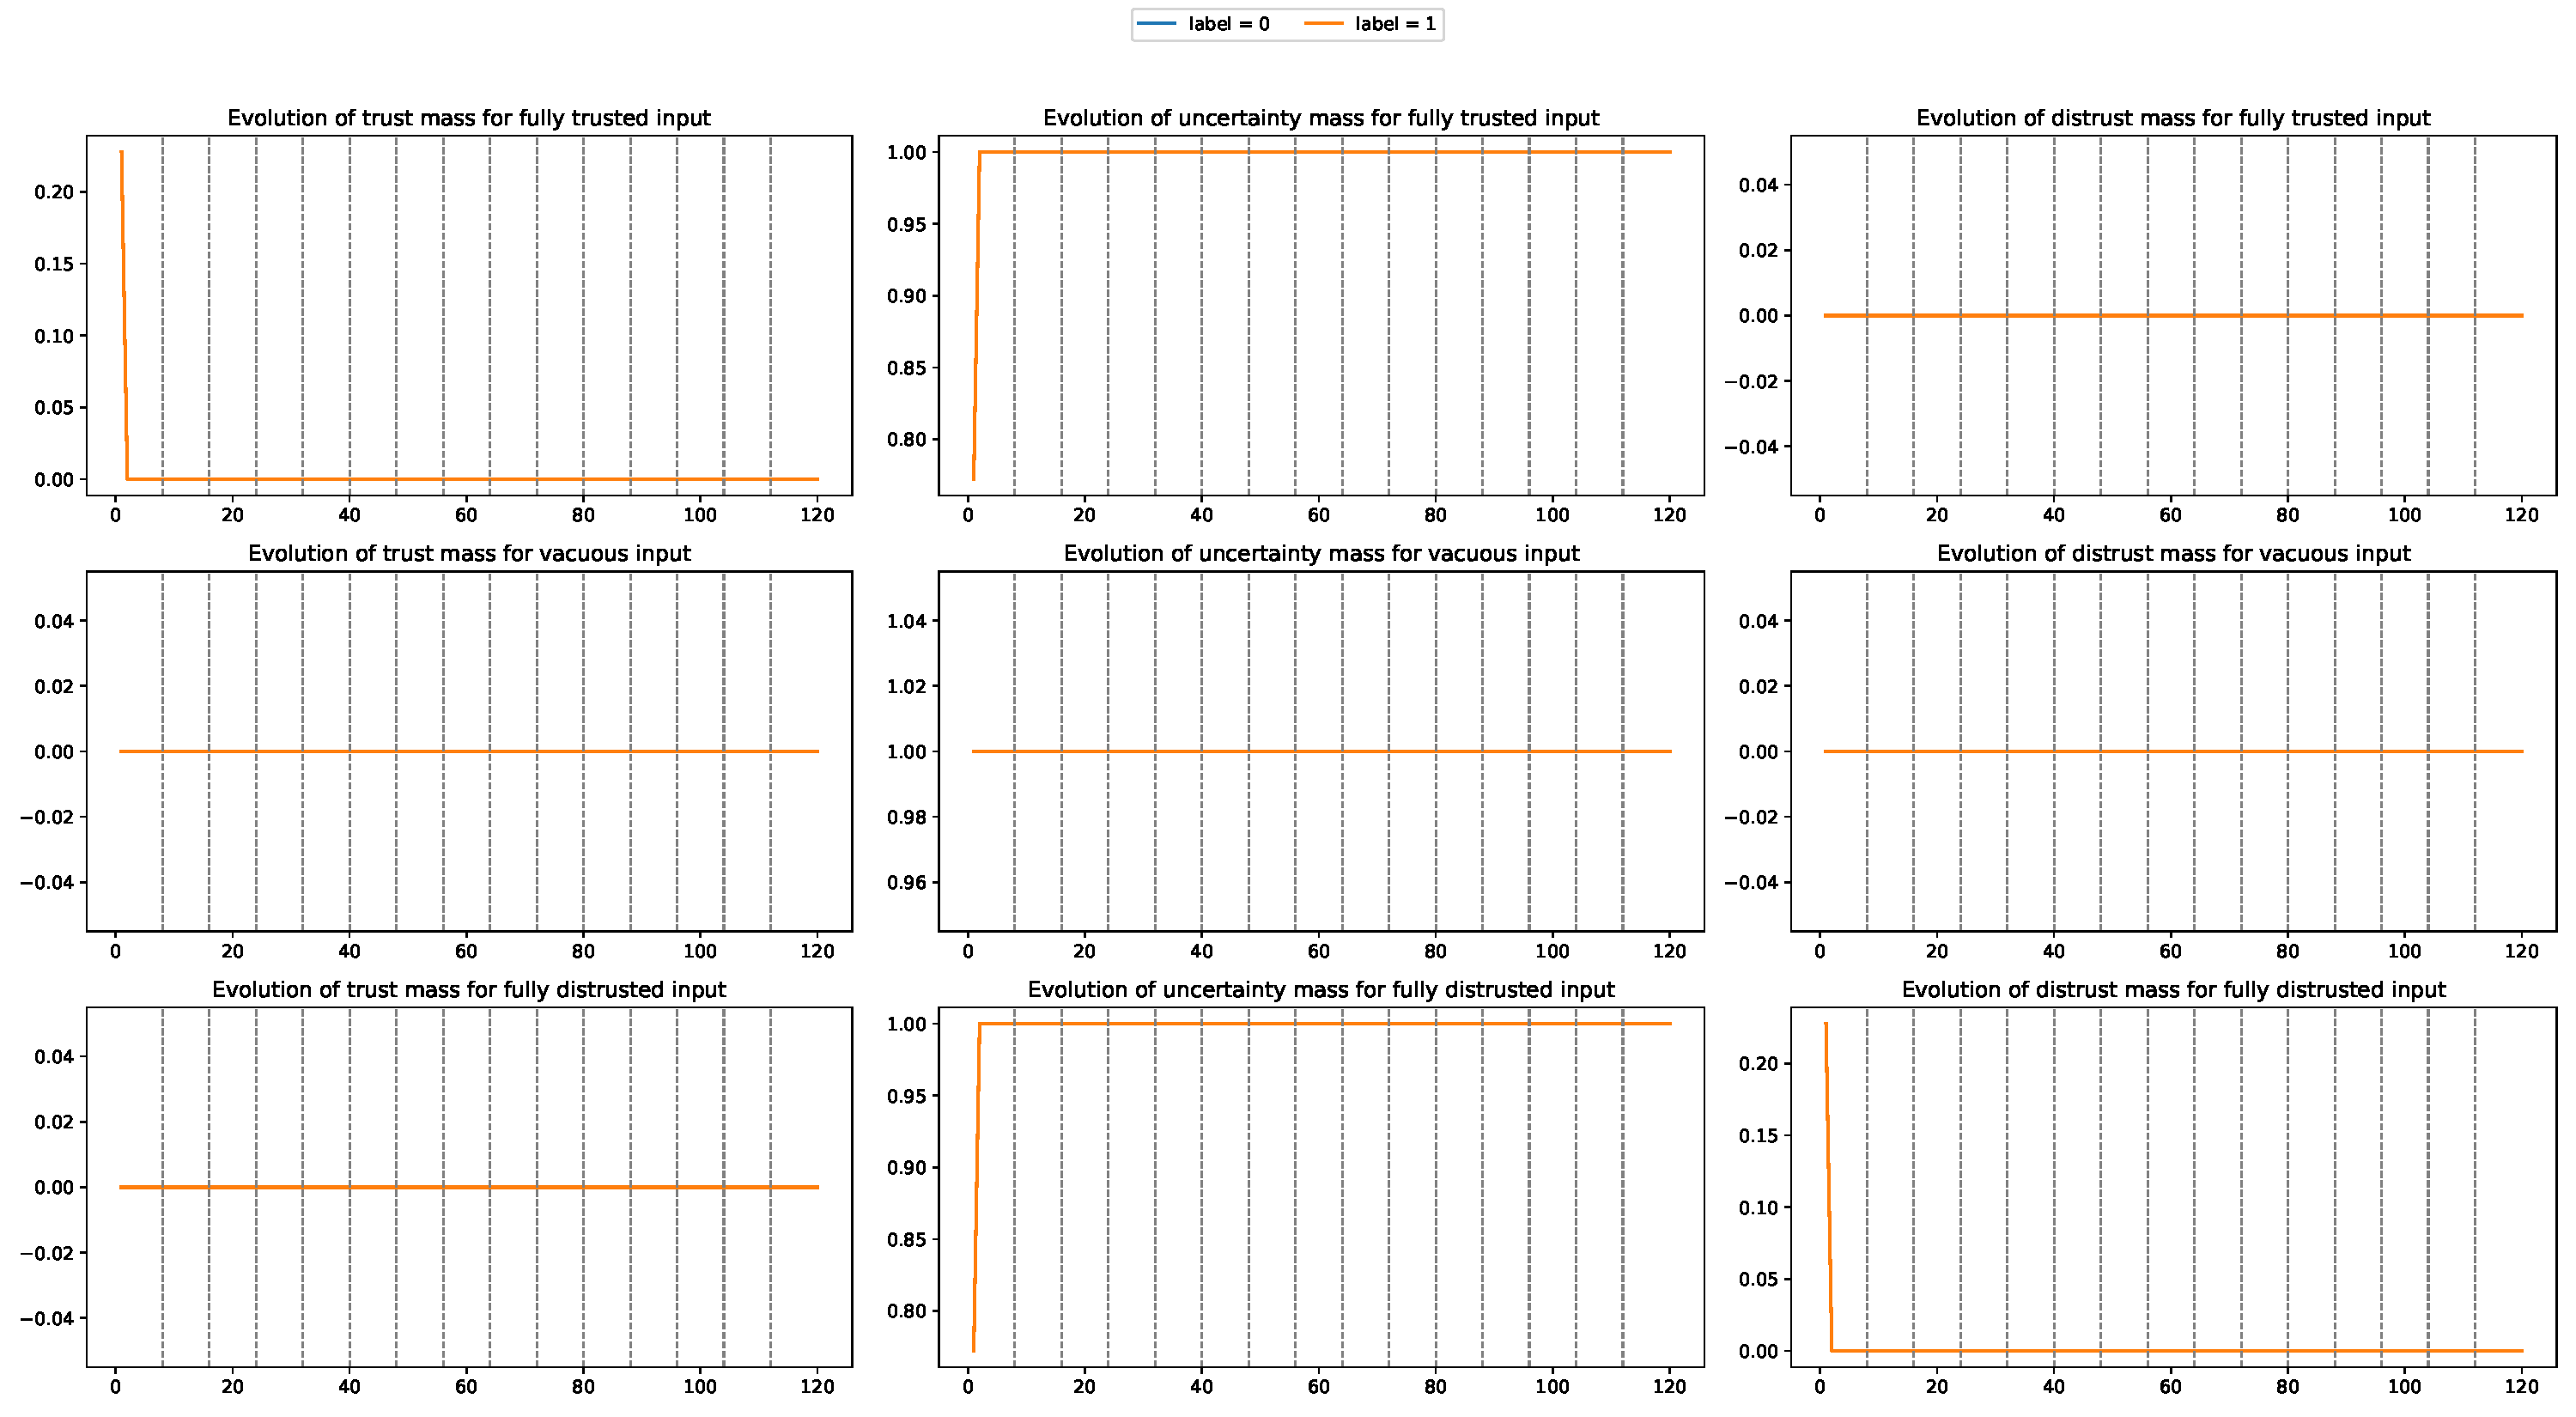
\includegraphics[width=0.8\textwidth]{latex/PTAS_Eval_cancer_16_distrust_vacuous_eps_1_PathSize_None__plot_ptas.pdf}
\caption{cancer\_16\_distrust\_vacuous, $\varepsilon$=1}
\end{figure}

\subsubsection{trust -- distrust}

\begin{figure}[htbp]
\centering
  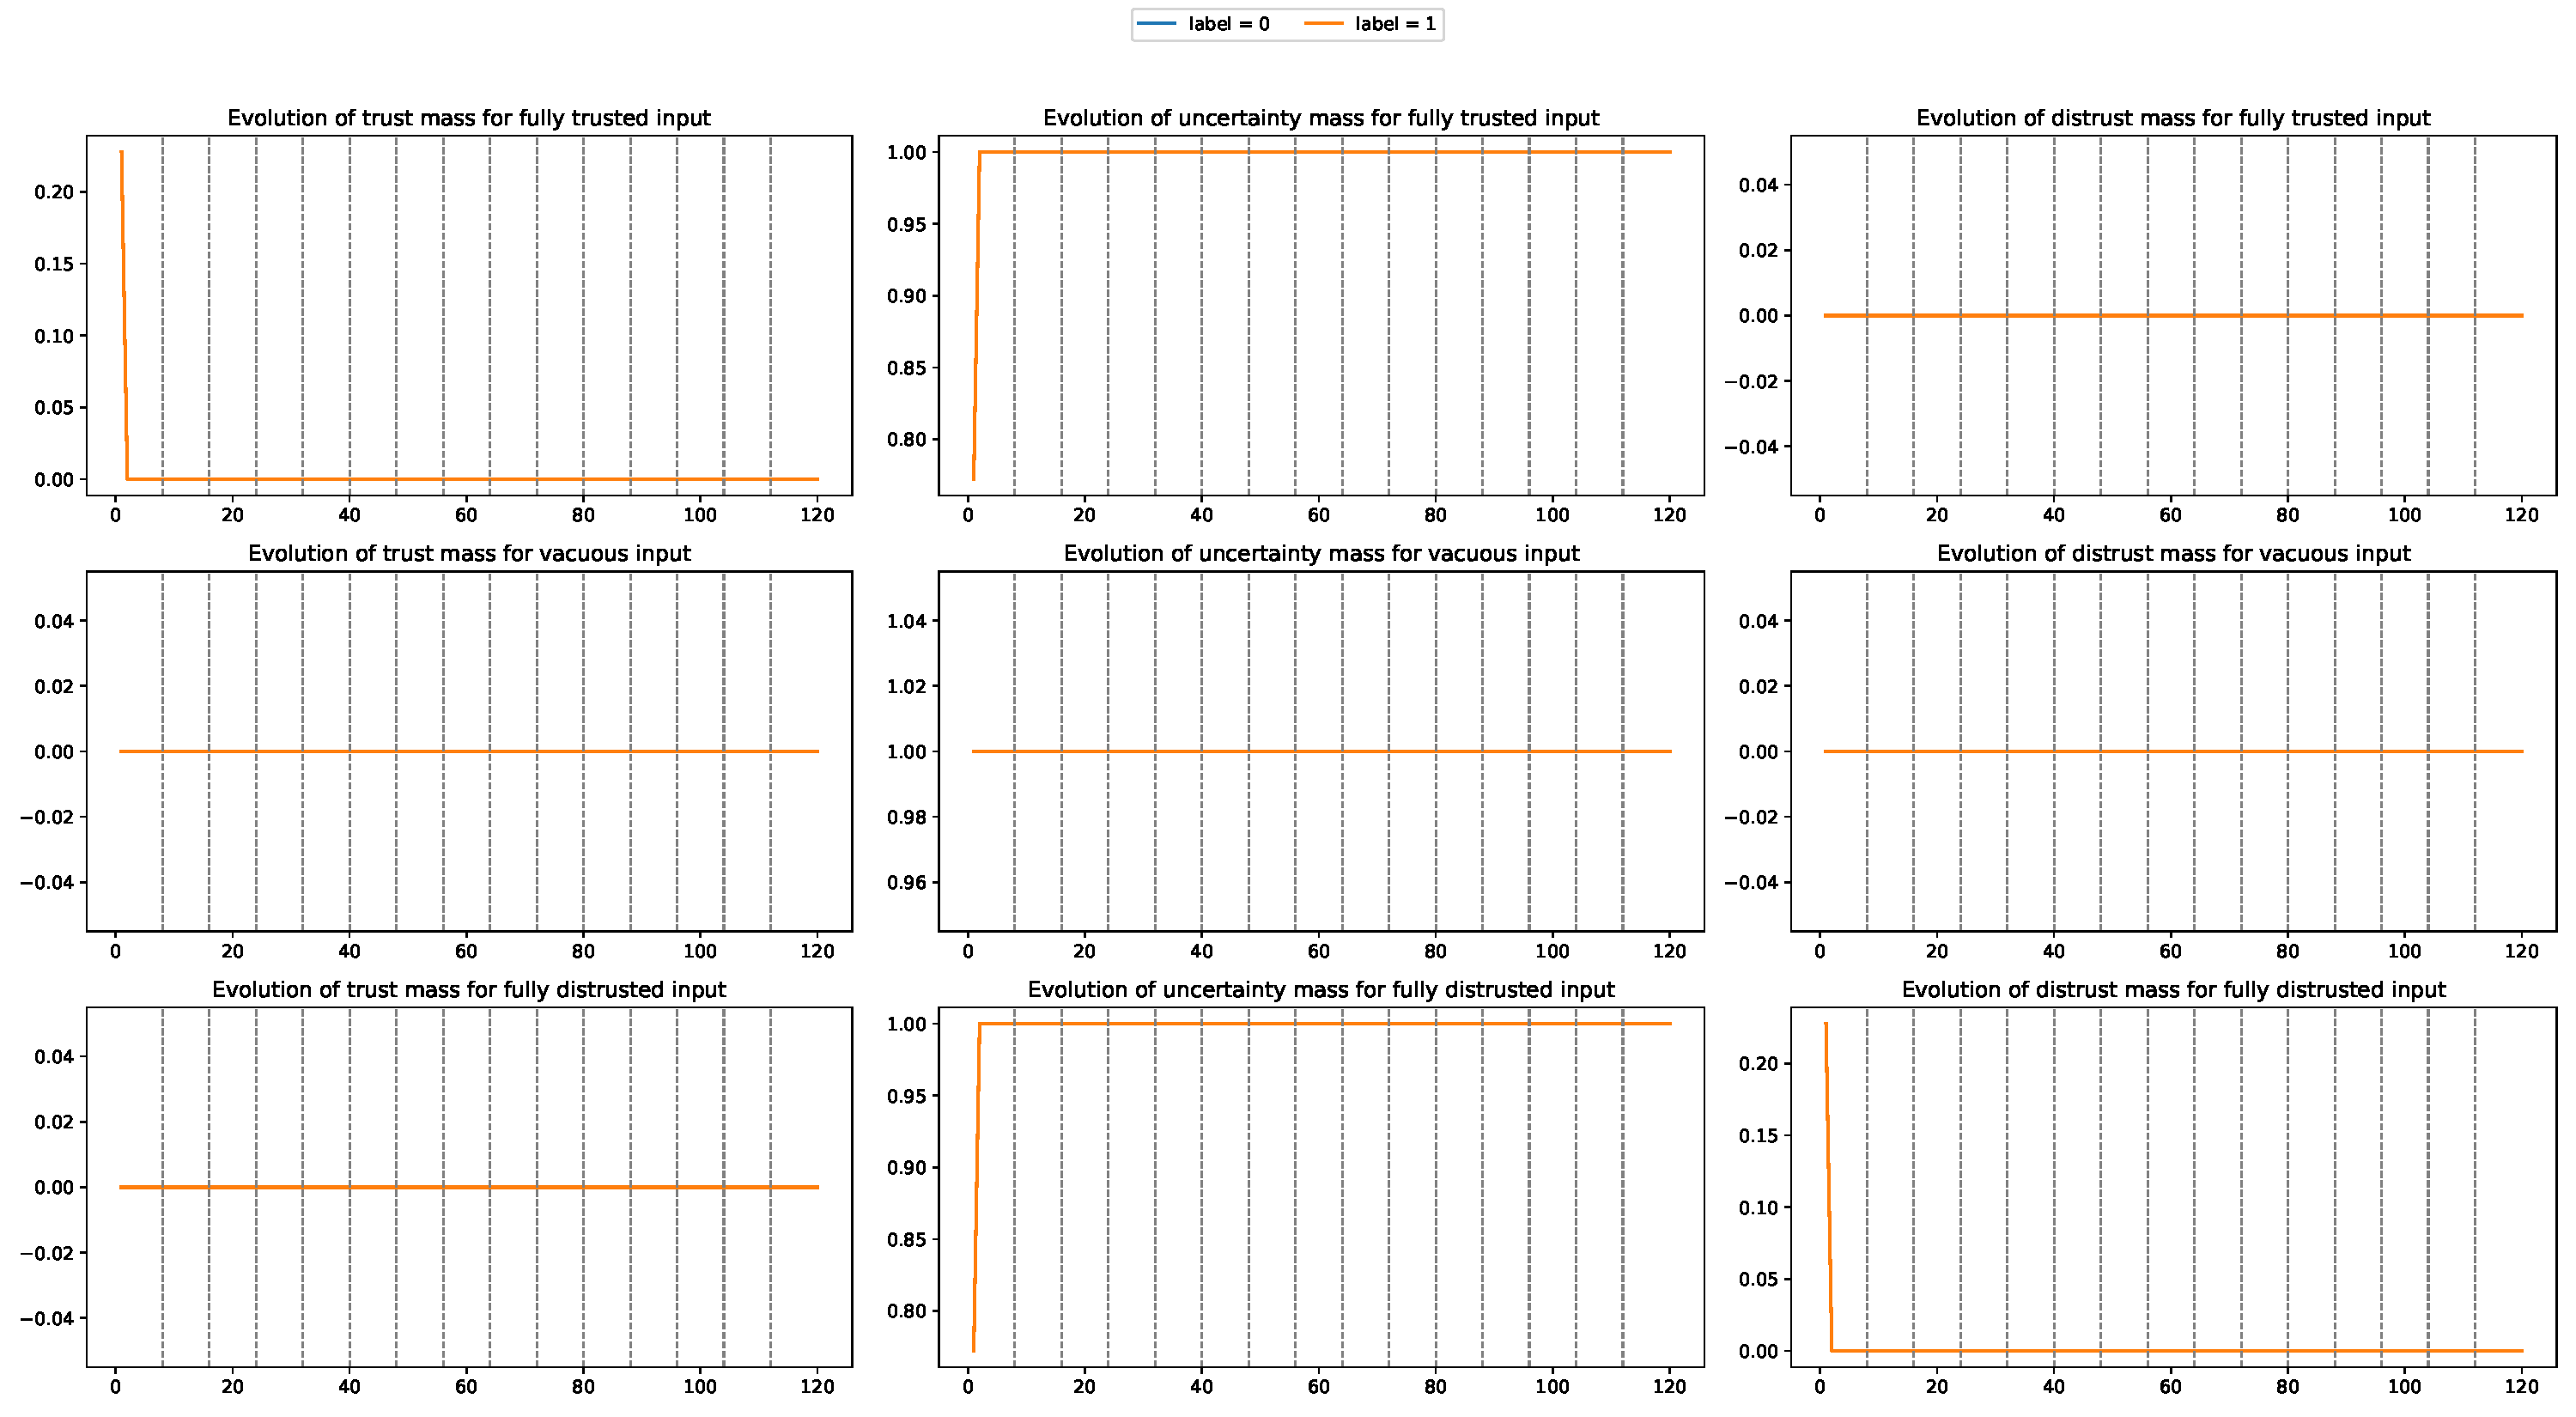
\includegraphics[width=0.8\textwidth]{latex/PTAS_Eval_cancer_16_trust_distrust_eps_0.001_PathSize_None__plot_ptas.pdf}
\caption{cancer\_16\_trust\_distrust, $\varepsilon$=0.001}
\end{figure}

\begin{figure}[htbp]
\centering
  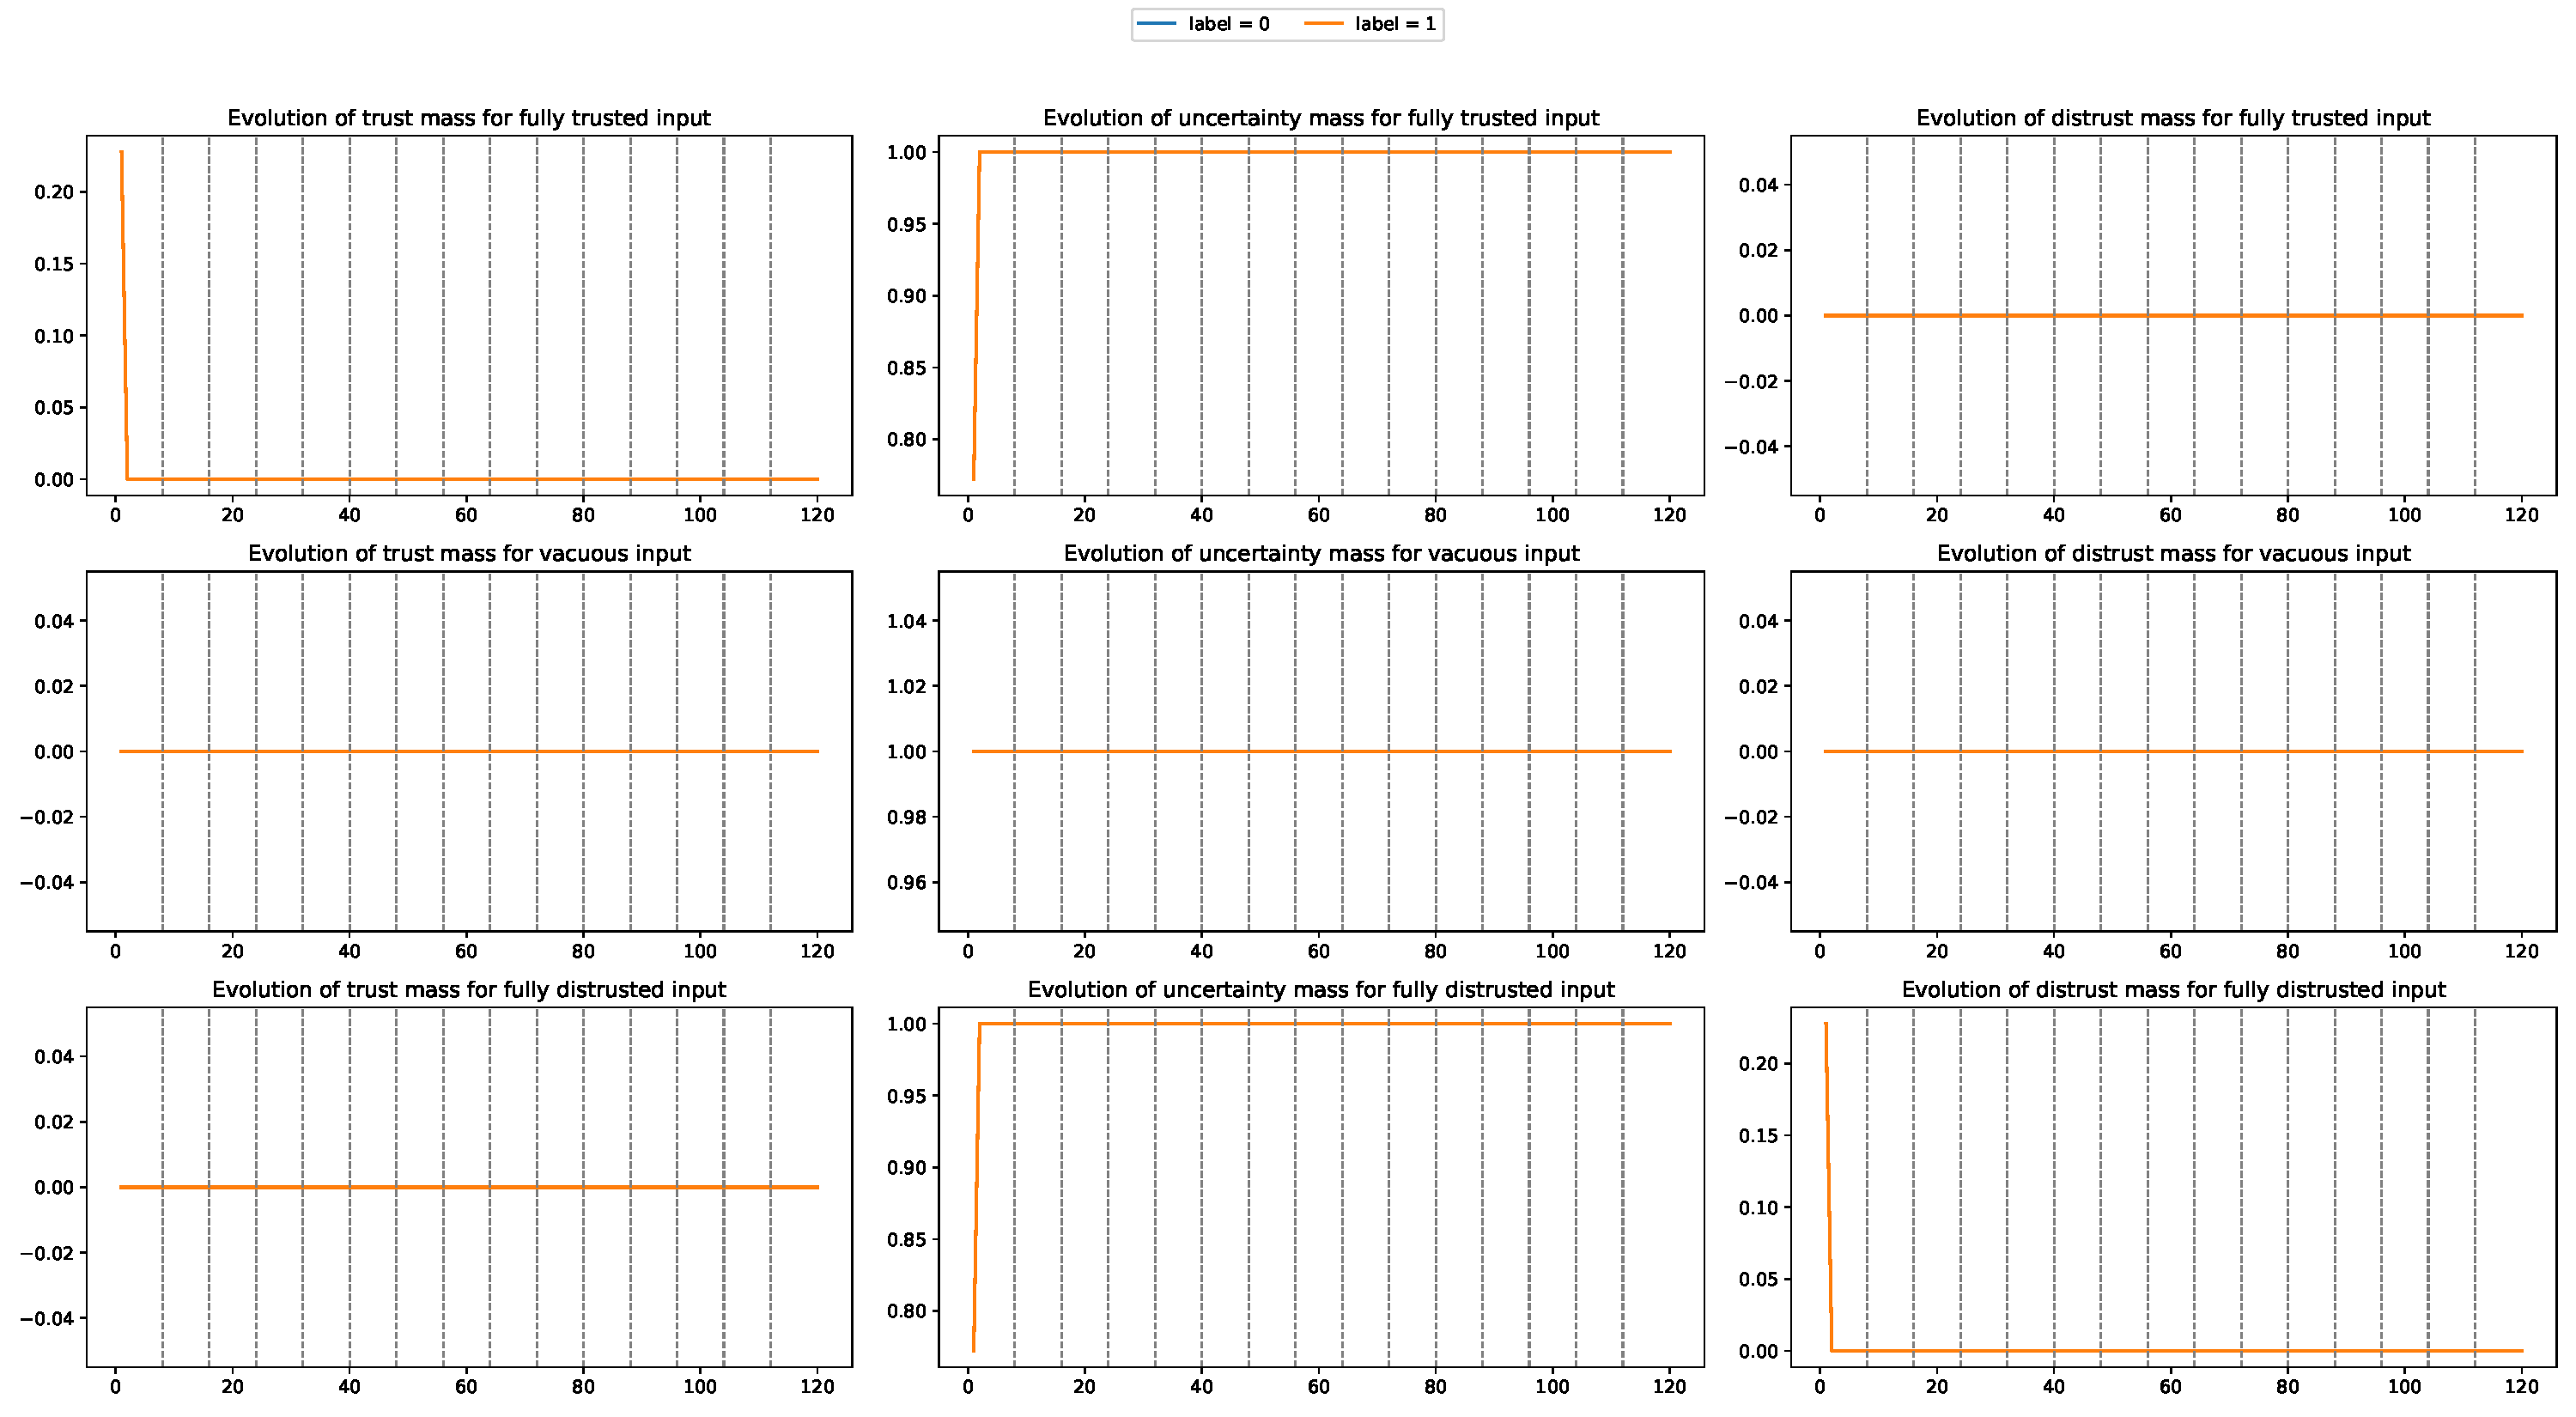
\includegraphics[width=0.8\textwidth]{latex/PTAS_Eval_cancer_16_trust_distrust_eps_0.01_PathSize_None__plot_ptas.pdf}
\caption{cancer\_16\_trust\_distrust, $\varepsilon$=0.01}
\end{figure}

\begin{figure}[htbp]
\centering
  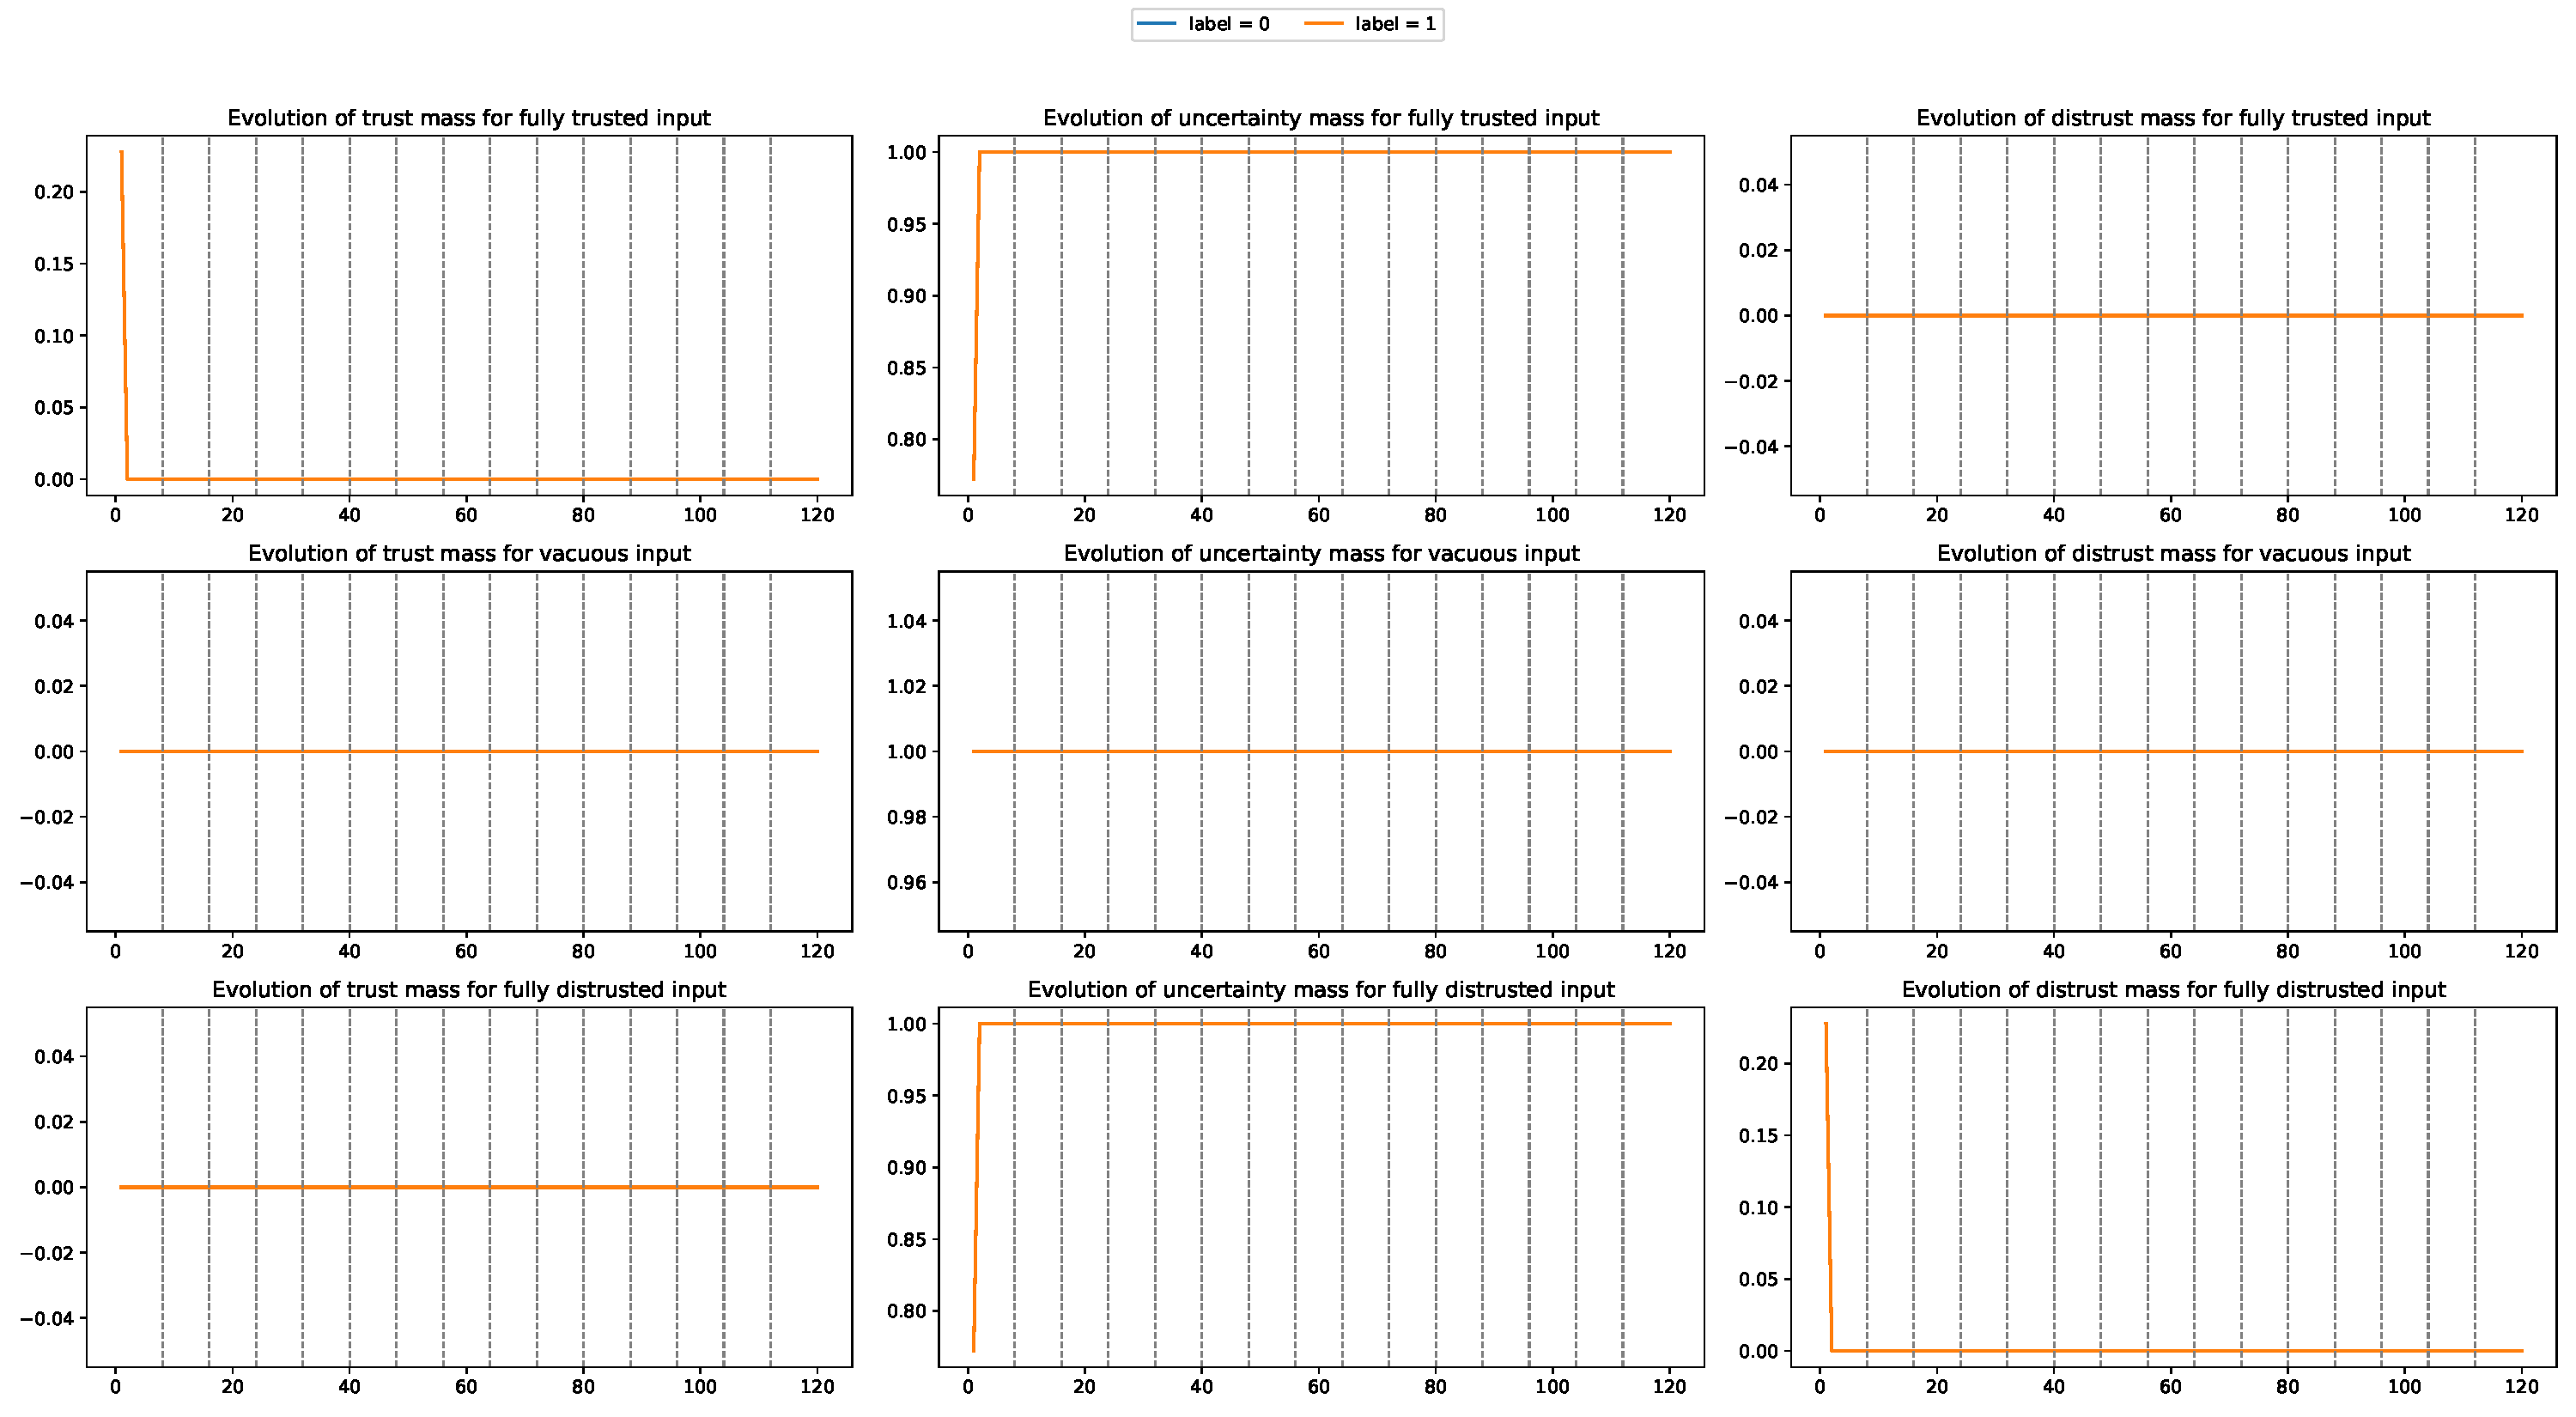
\includegraphics[width=0.8\textwidth]{latex/PTAS_Eval_cancer_16_trust_distrust_eps_0.1_PathSize_None__plot_ptas.pdf}
\caption{cancer\_16\_trust\_distrust, $\varepsilon$=0.1}
\end{figure}

\begin{figure}[htbp]
\centering
  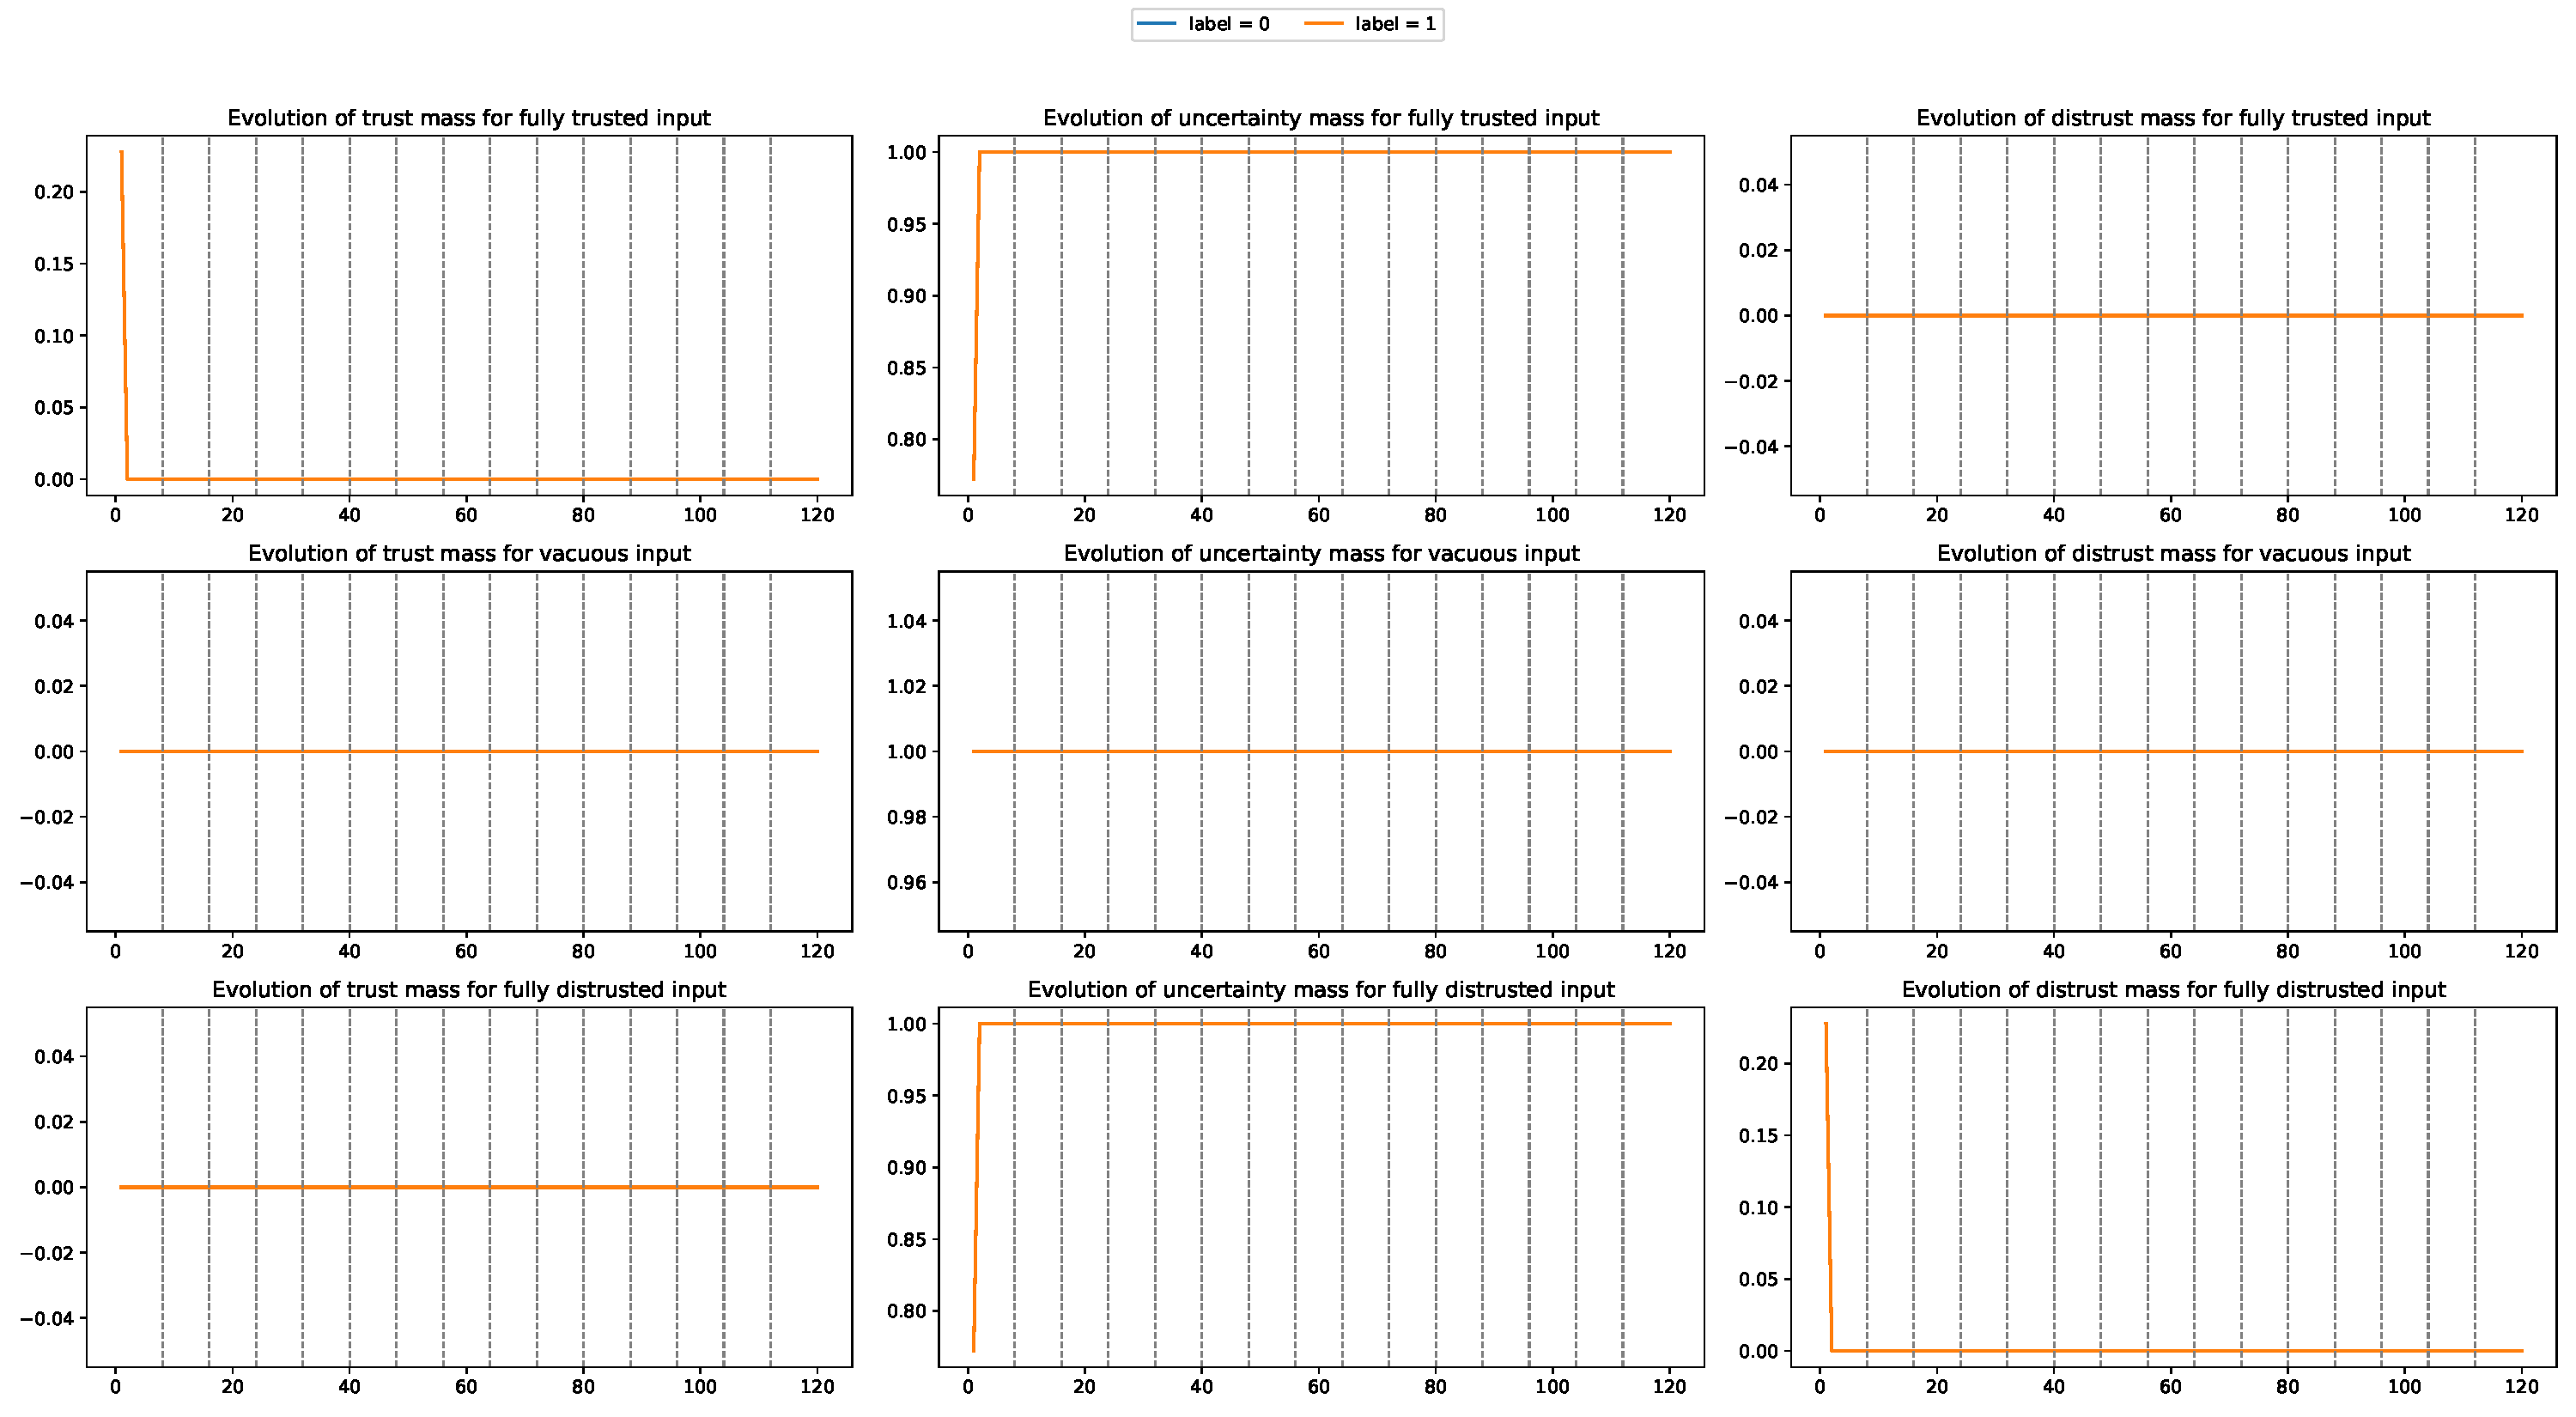
\includegraphics[width=0.8\textwidth]{latex/PTAS_Eval_cancer_16_trust_distrust_eps_1_PathSize_None__plot_ptas.pdf}
\caption{cancer\_16\_trust\_distrust, $\varepsilon$=1}
\end{figure}

\subsubsection{trust -- trust}

\begin{figure}[htbp]
\centering
  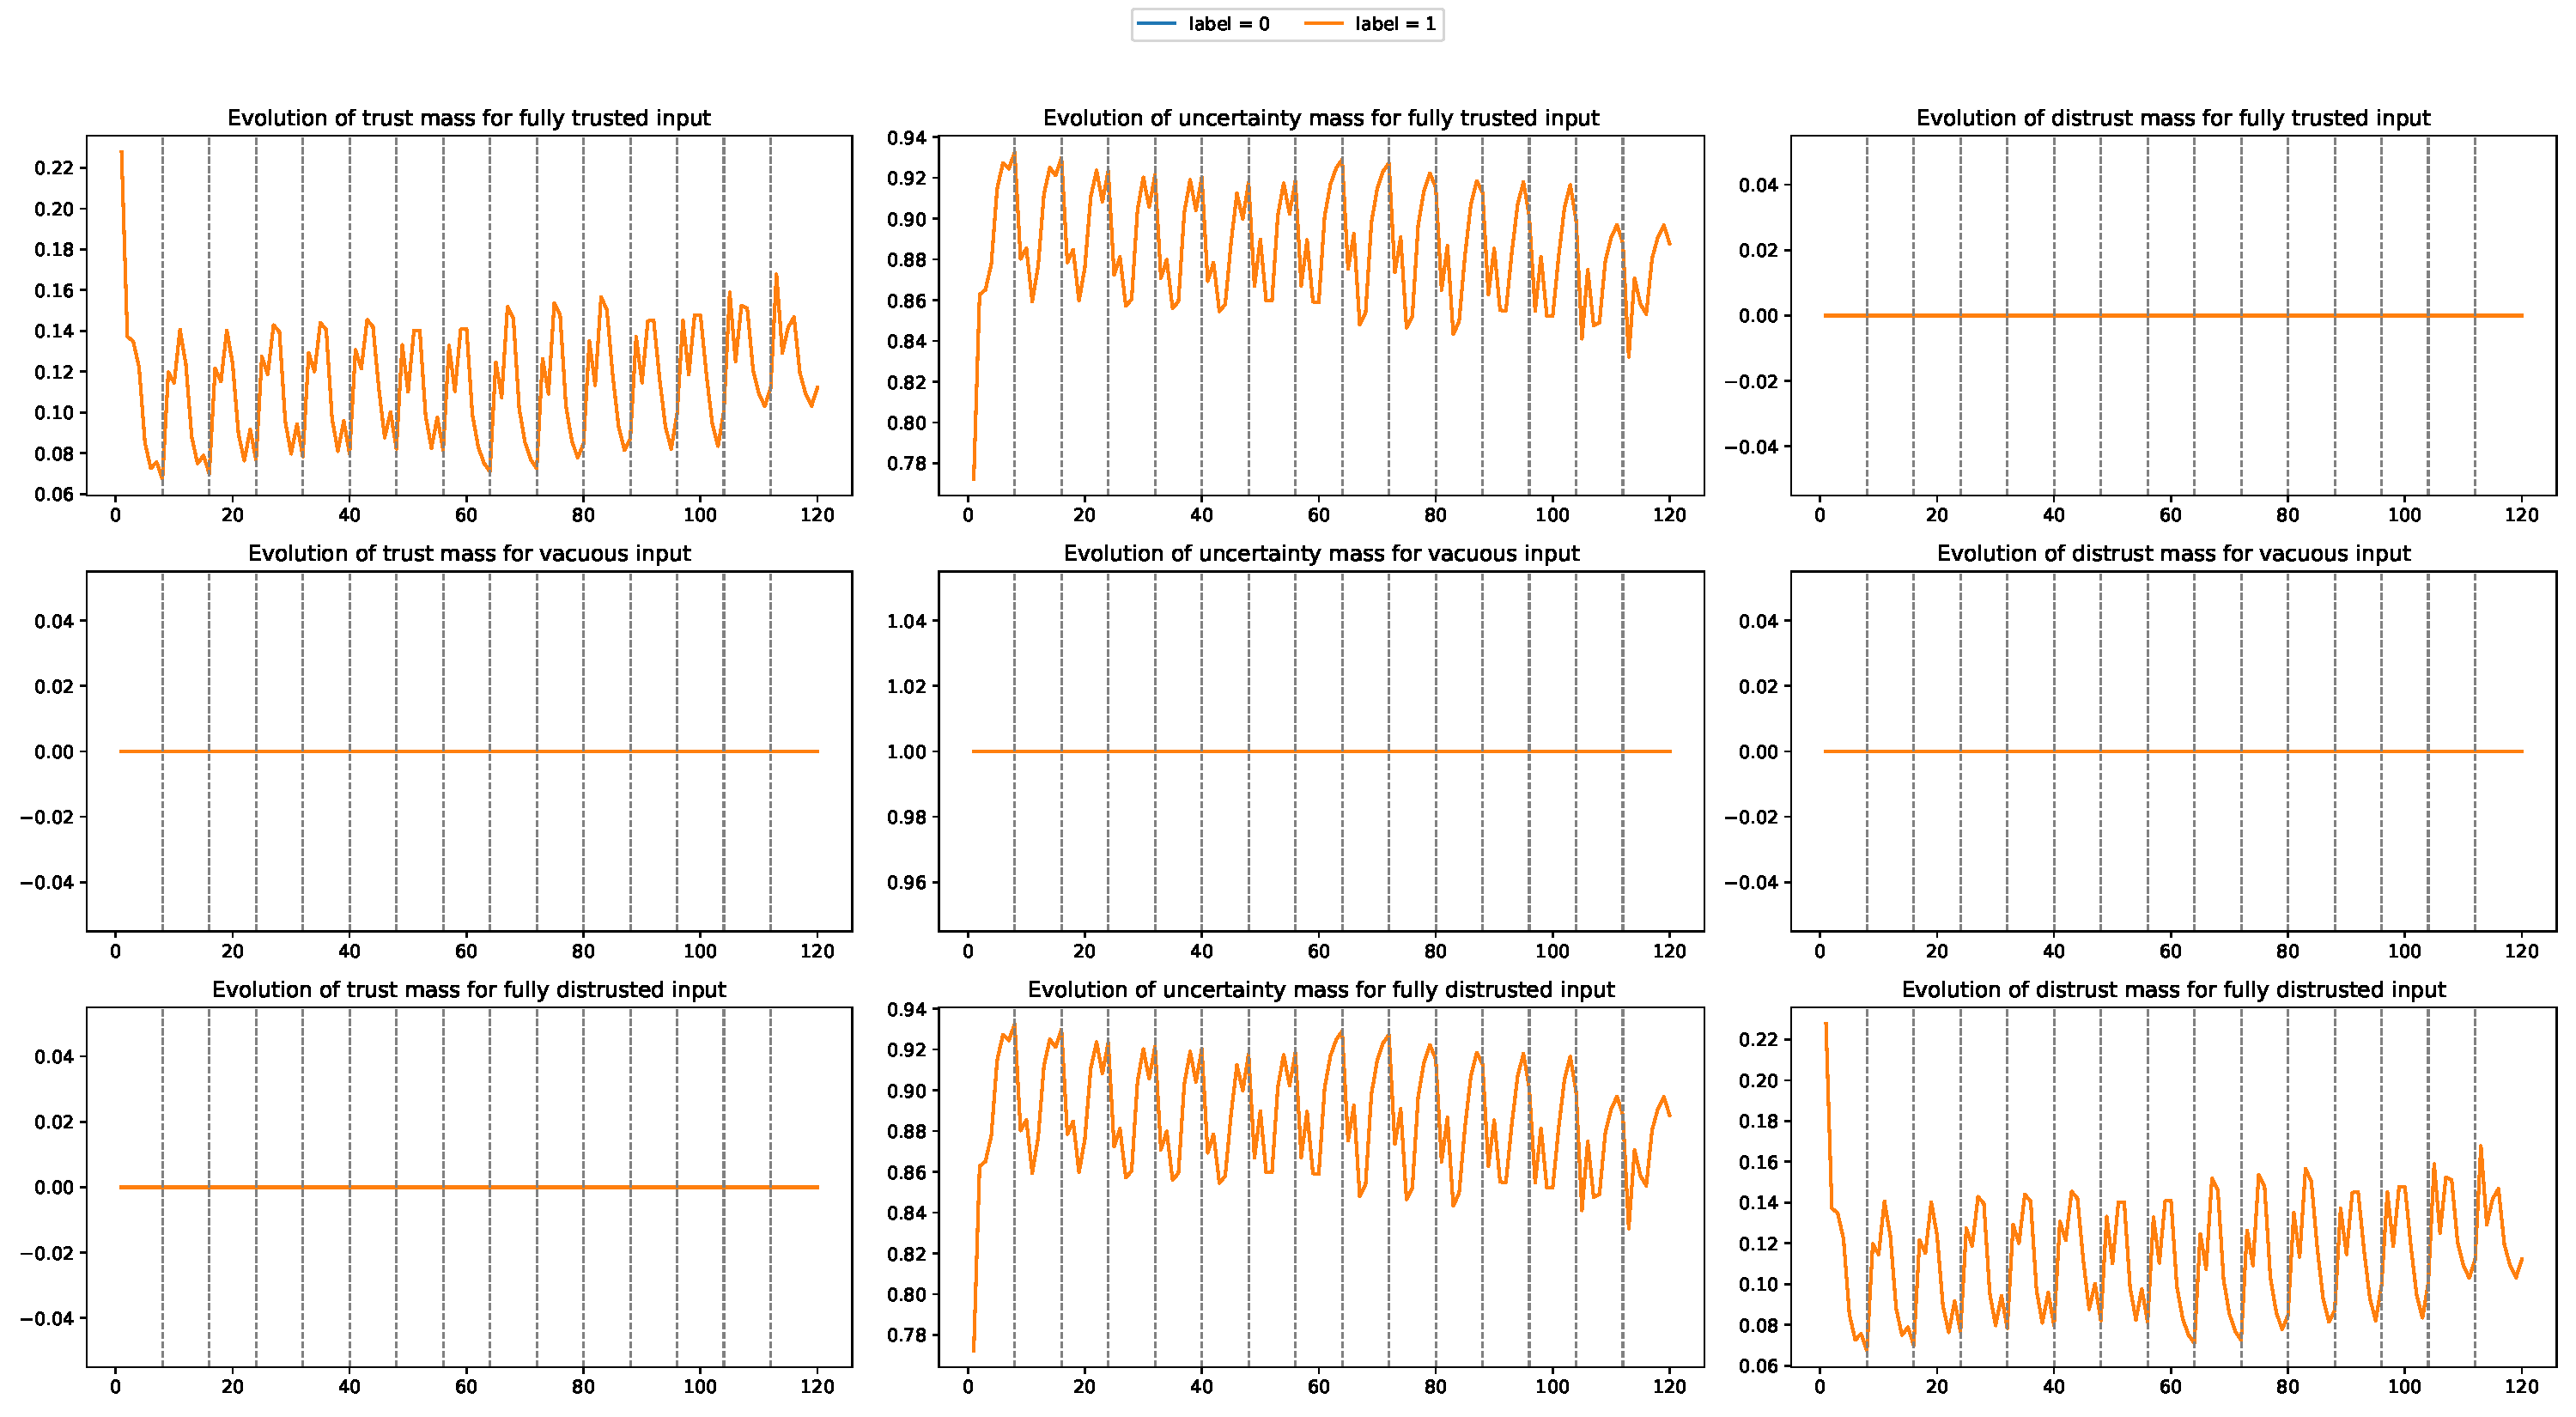
\includegraphics[width=0.8\textwidth]{latex/PTAS_Eval_cancer_16_trust_trust_eps_0.001_PathSize_None__plot_ptas.pdf}
\caption{cancer\_16\_trust\_trust, $\varepsilon$=0.001}
\end{figure}

\begin{figure}[htbp]
\centering
  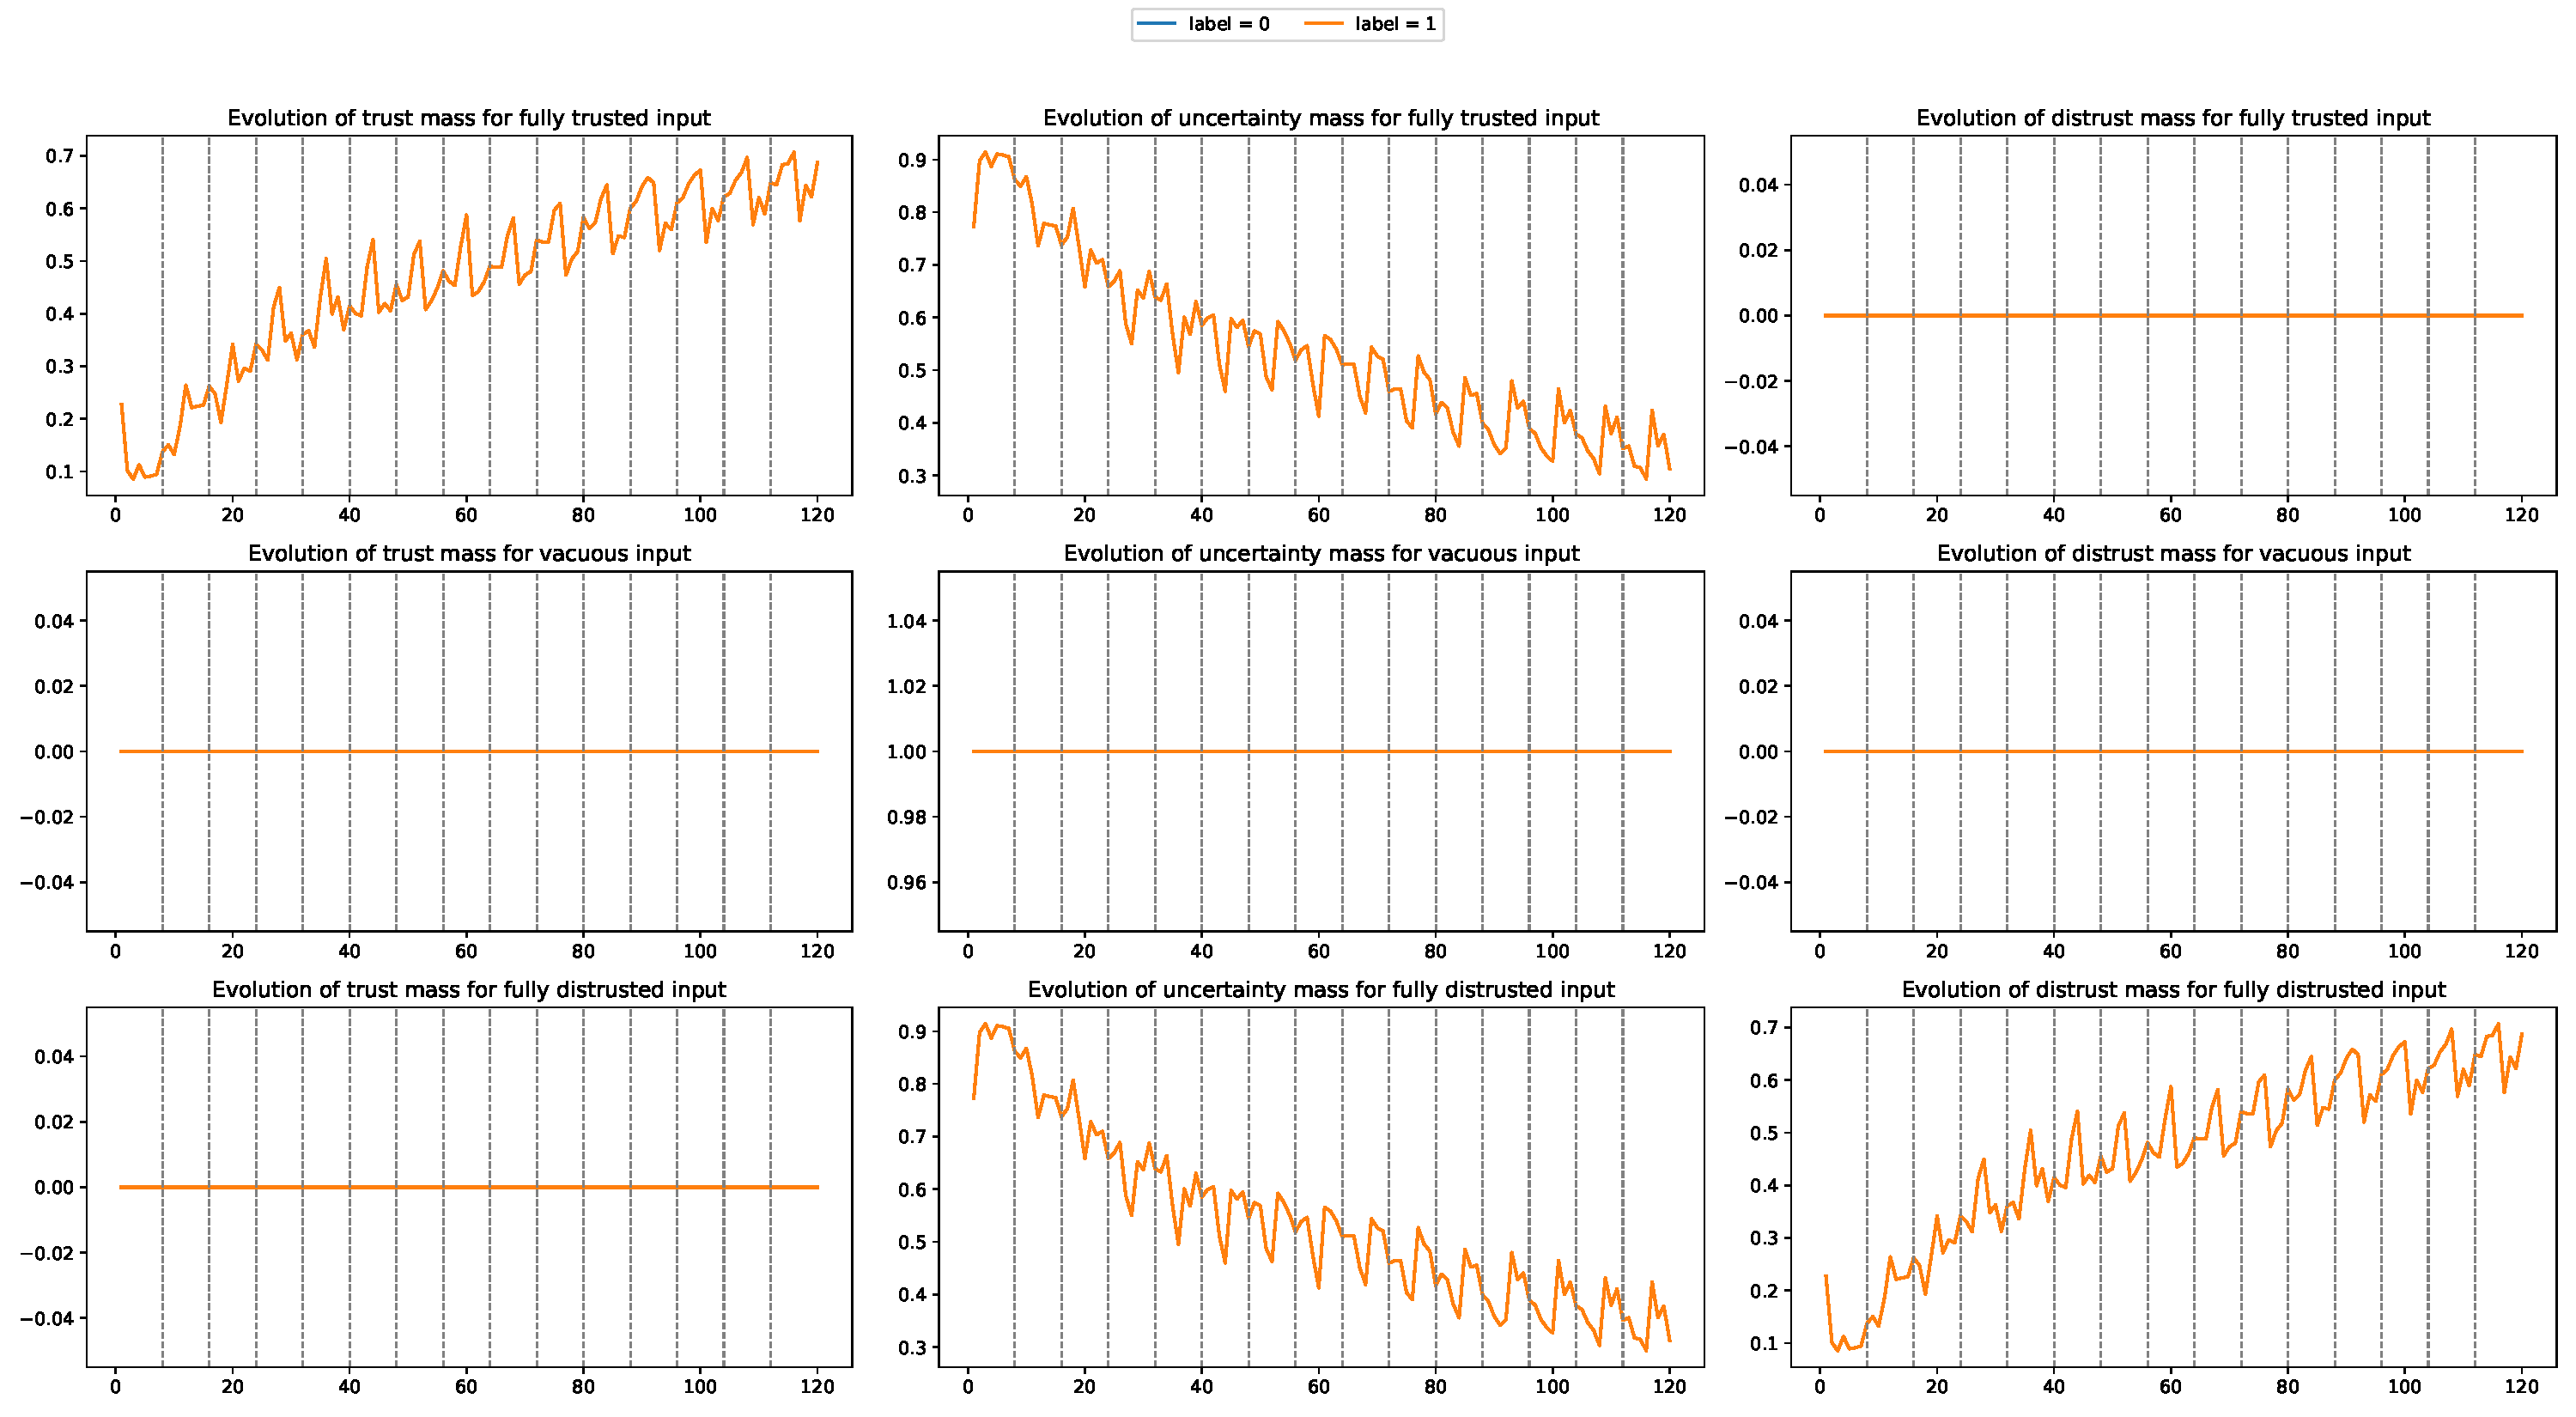
\includegraphics[width=0.8\textwidth]{latex/PTAS_Eval_cancer_16_trust_trust_eps_0.01_PathSize_None__plot_ptas.pdf}
\caption{cancer\_16\_trust\_trust, $\varepsilon$=0.01}
\end{figure}

\begin{figure}[htbp]
\centering
  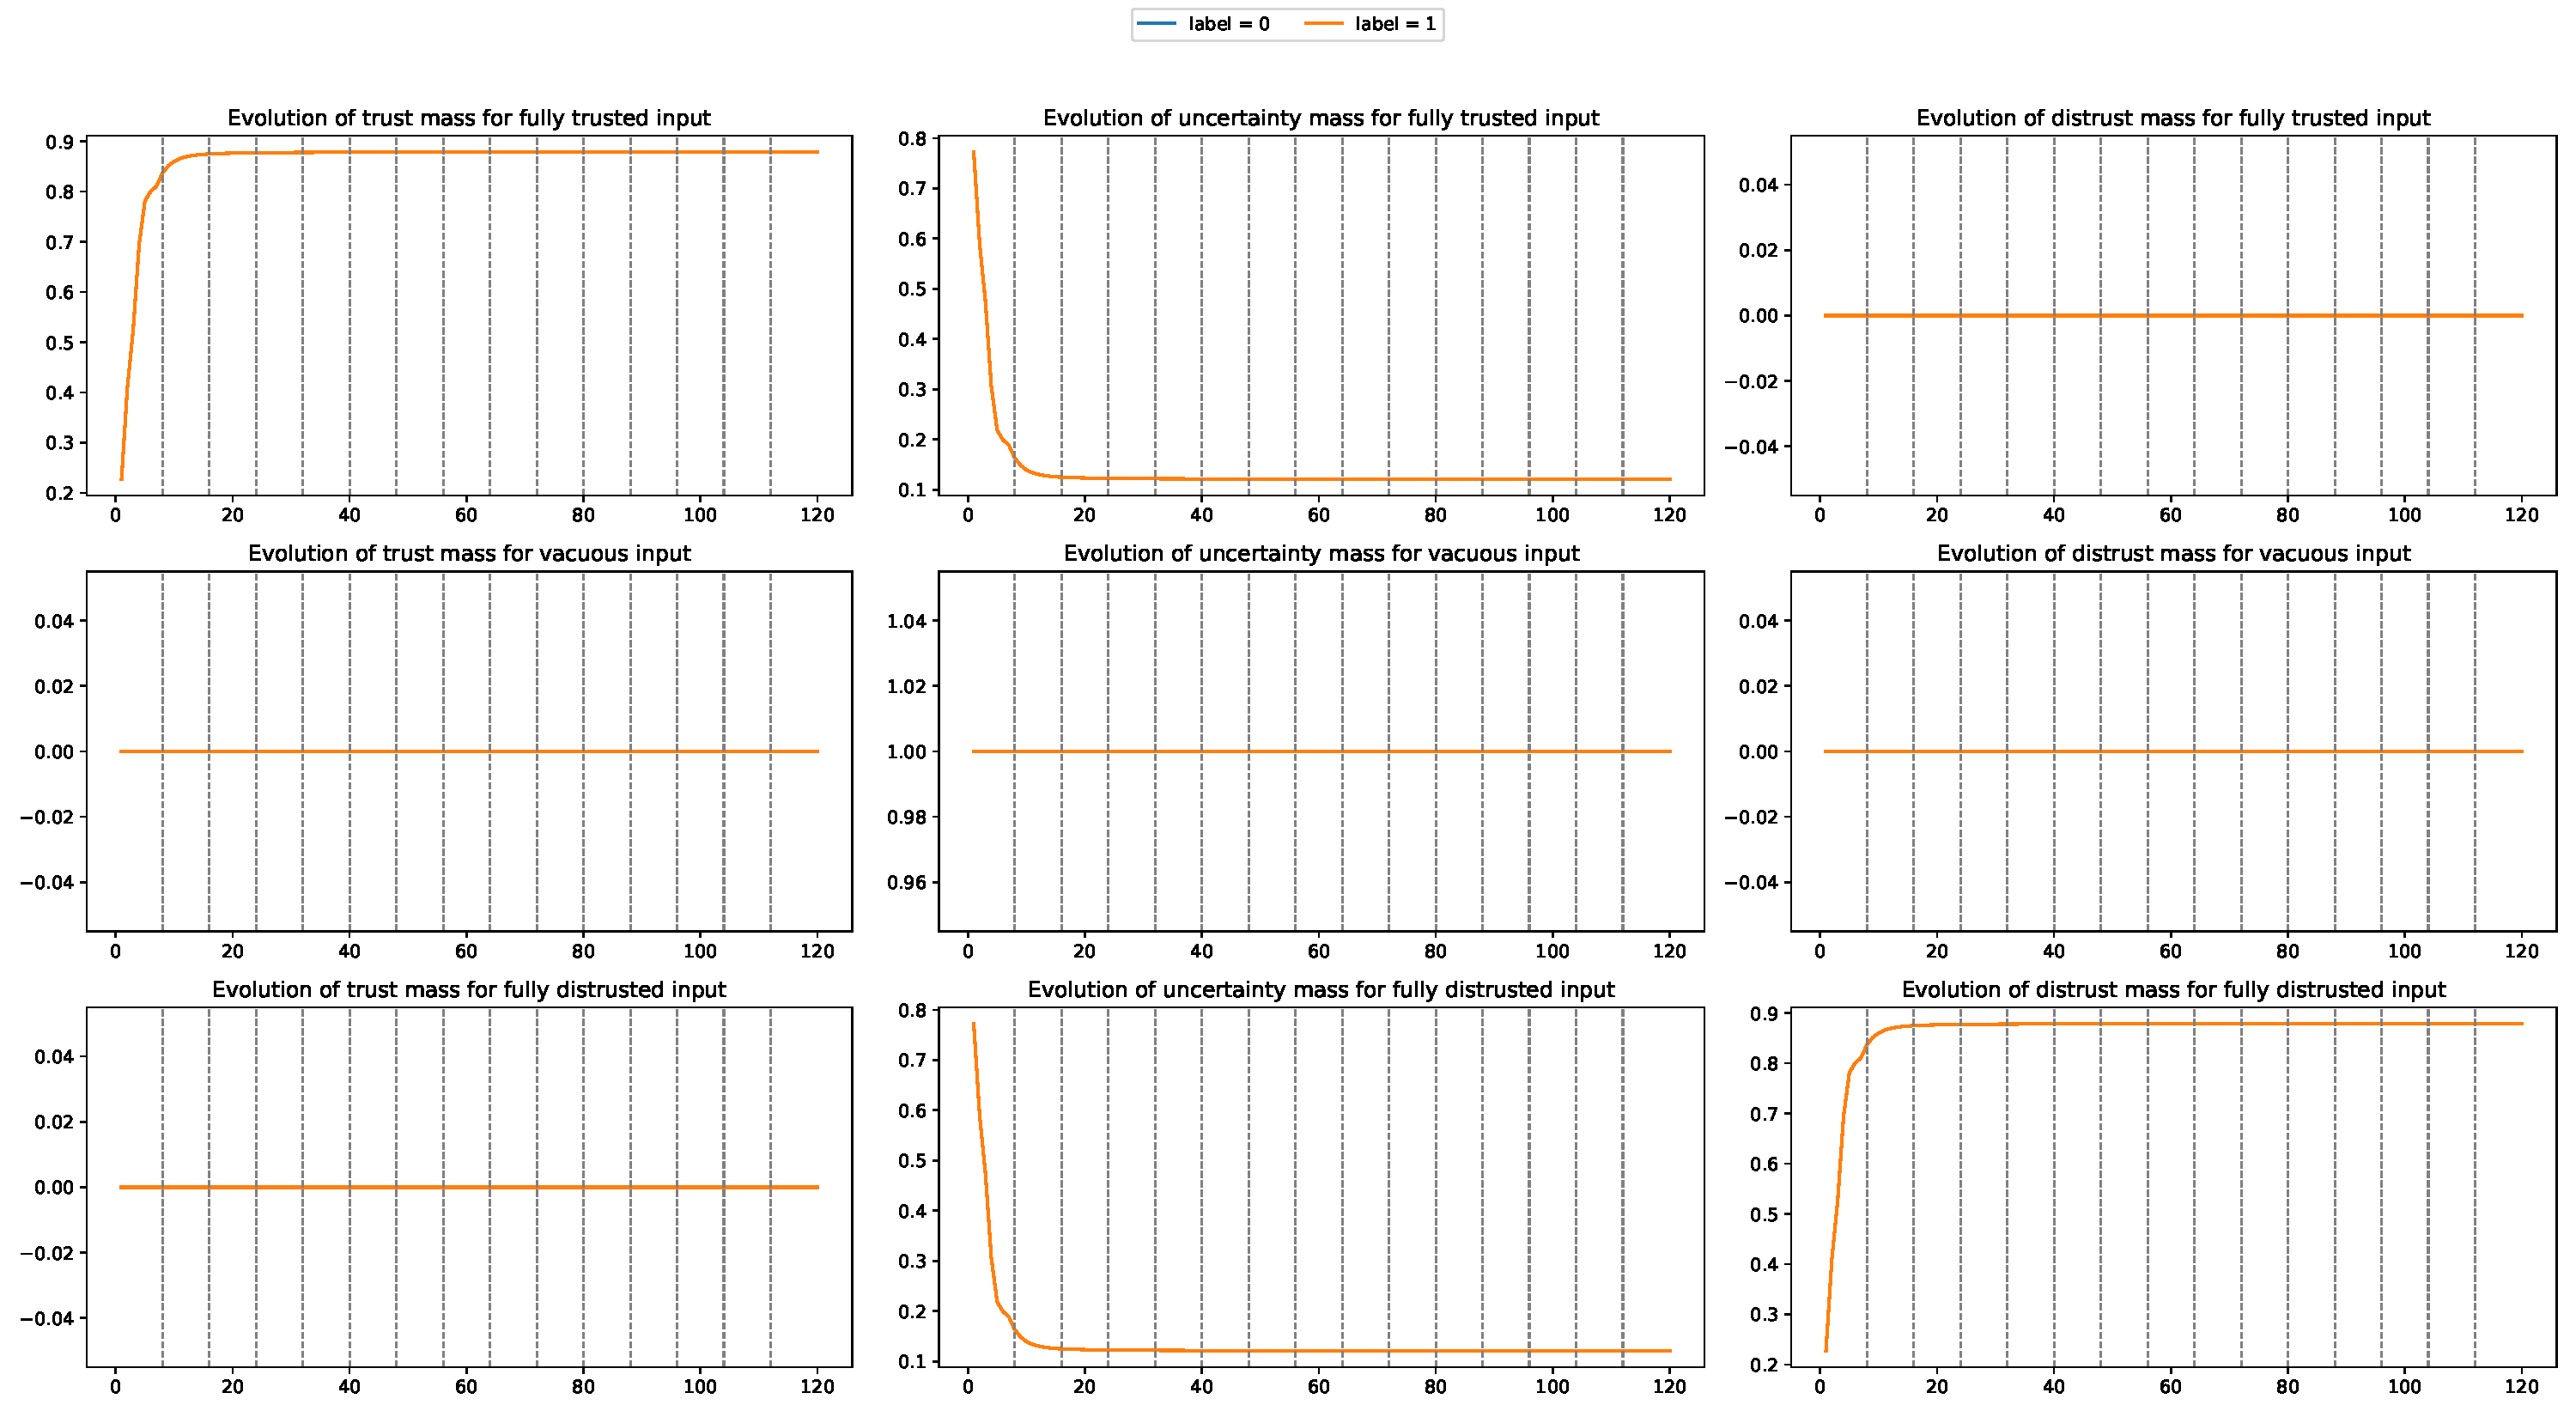
\includegraphics[width=0.8\textwidth]{latex/PTAS_Eval_cancer_16_trust_trust_eps_0.1_PathSize_None__plot_ptas.pdf}
\caption{cancer\_16\_trust\_trust, $\varepsilon$=0.1}
\end{figure}

\begin{figure}[htbp]
\centering
  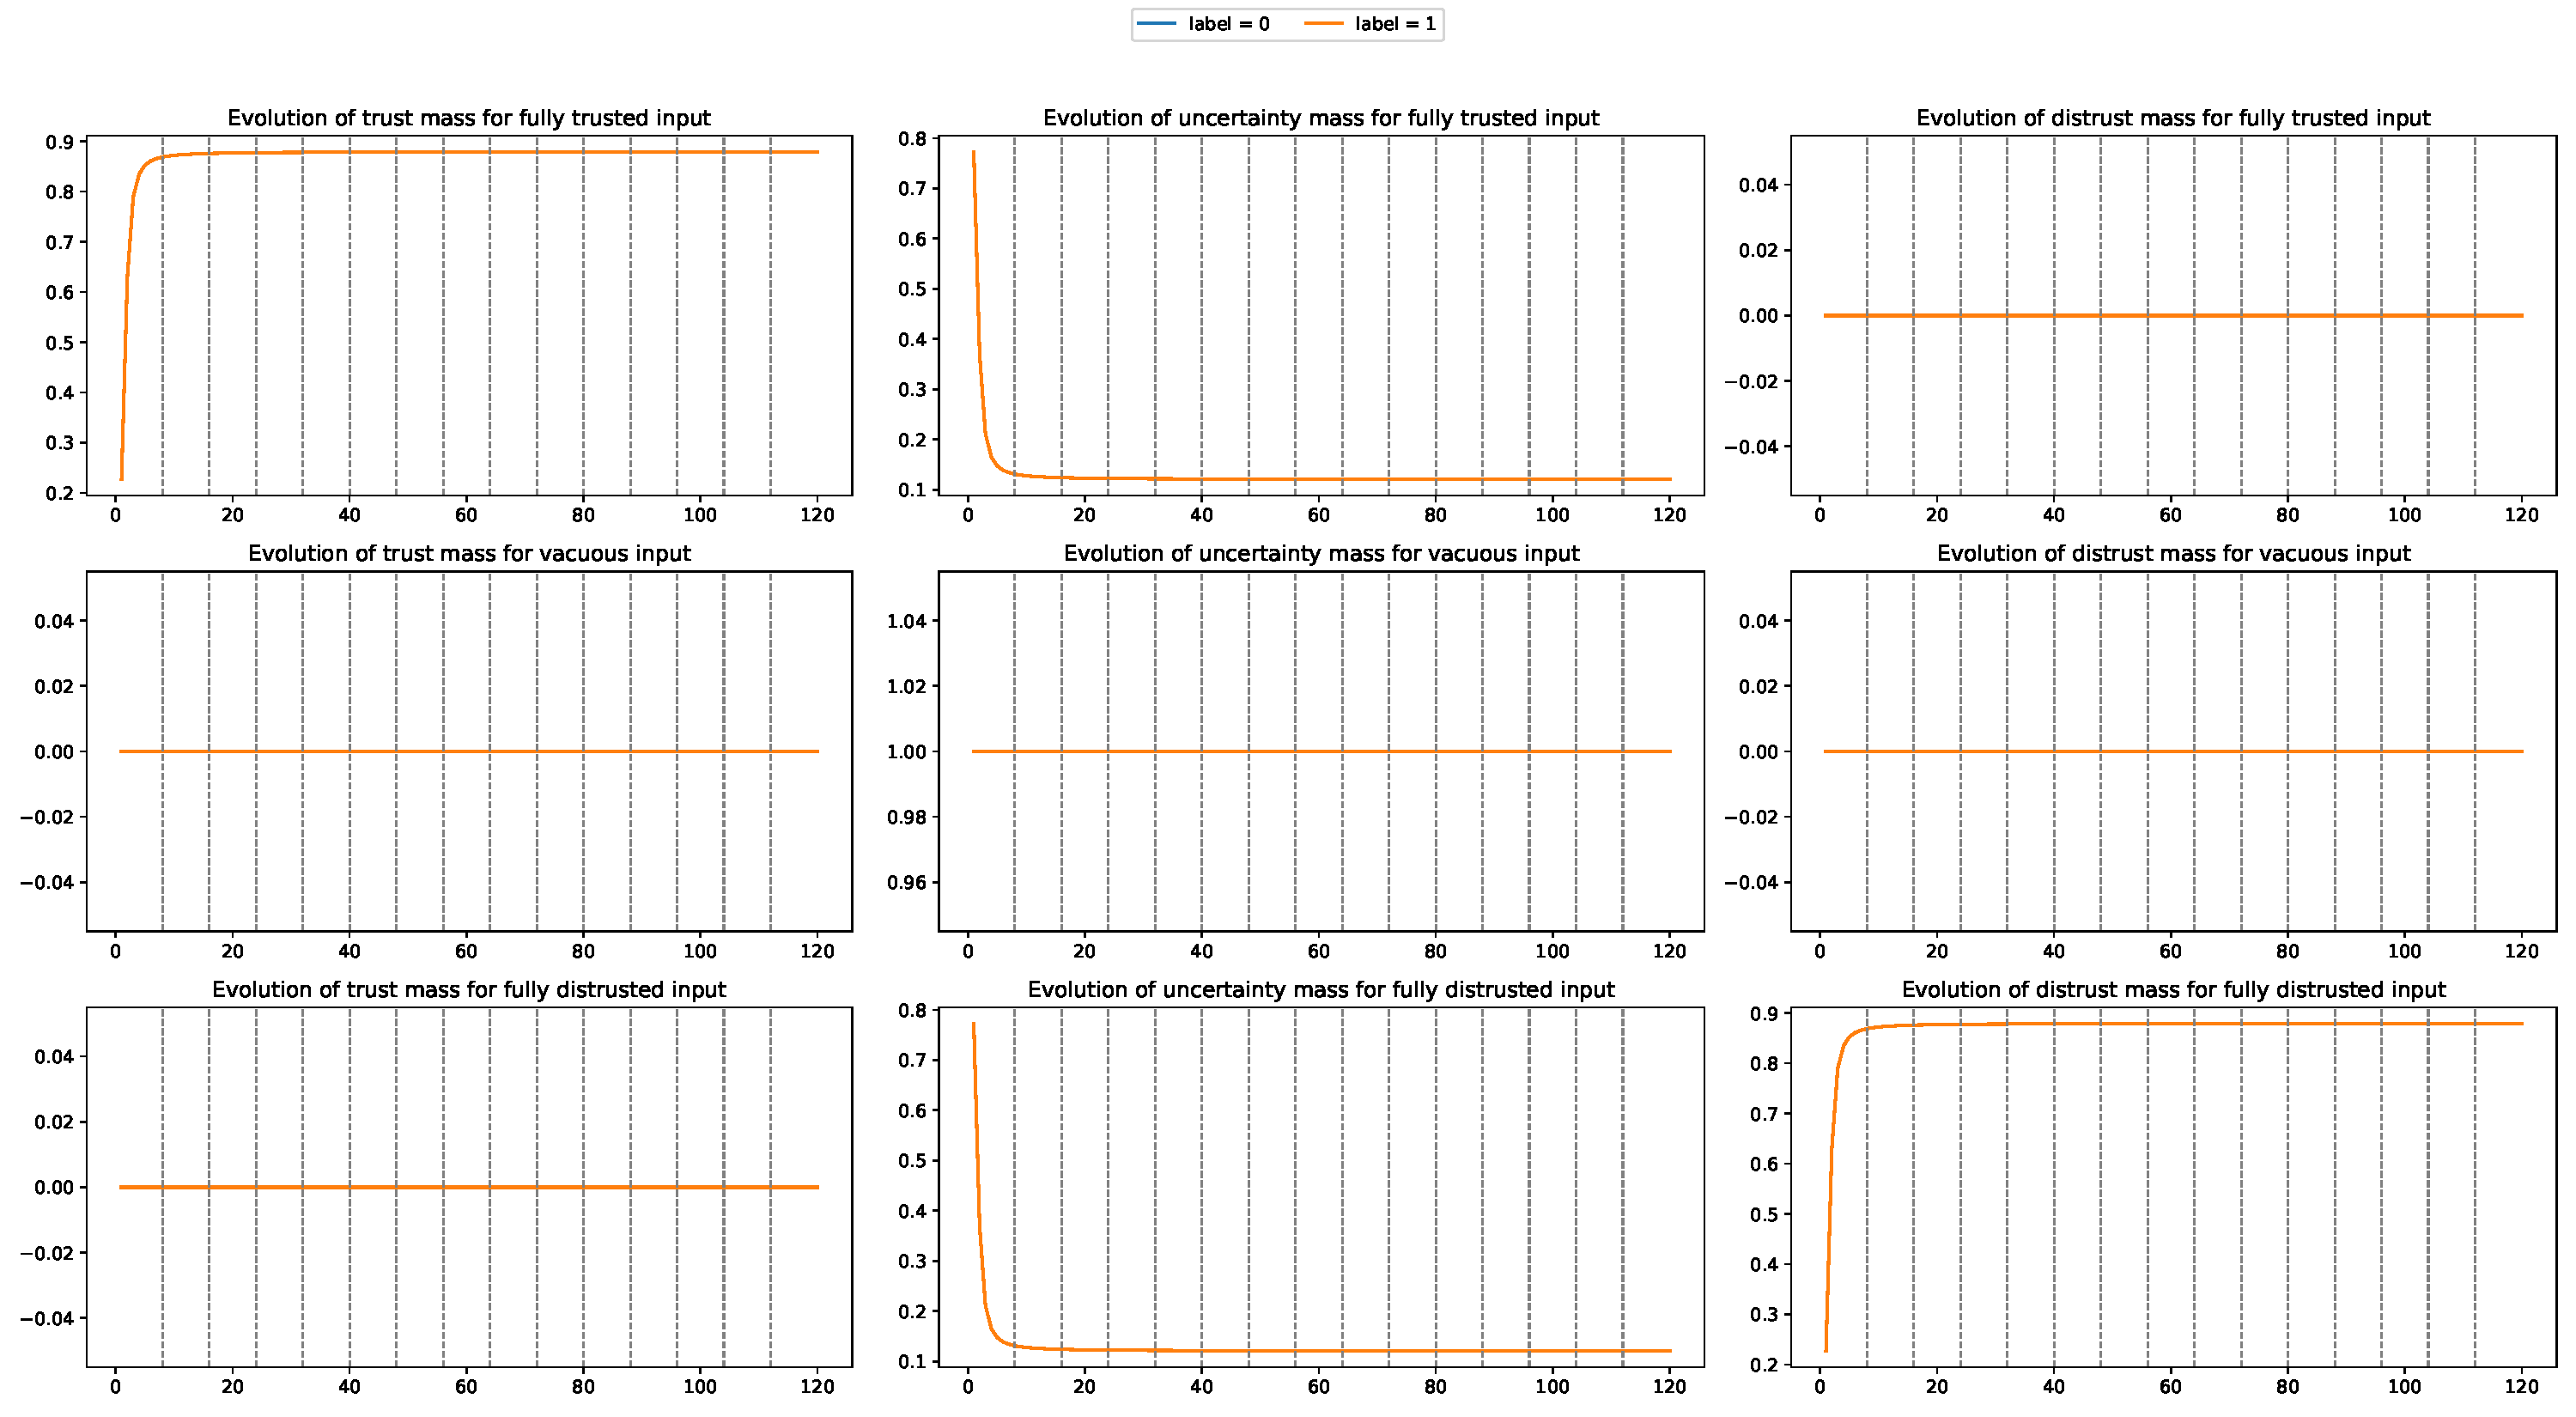
\includegraphics[width=0.8\textwidth]{latex/PTAS_Eval_cancer_16_trust_trust_eps_1_PathSize_None__plot_ptas.pdf}
\caption{cancer\_16\_trust\_trust, $\varepsilon$=1}
\end{figure}

\subsubsection{trust -- vacuous}

\begin{figure}[htbp]
\centering
  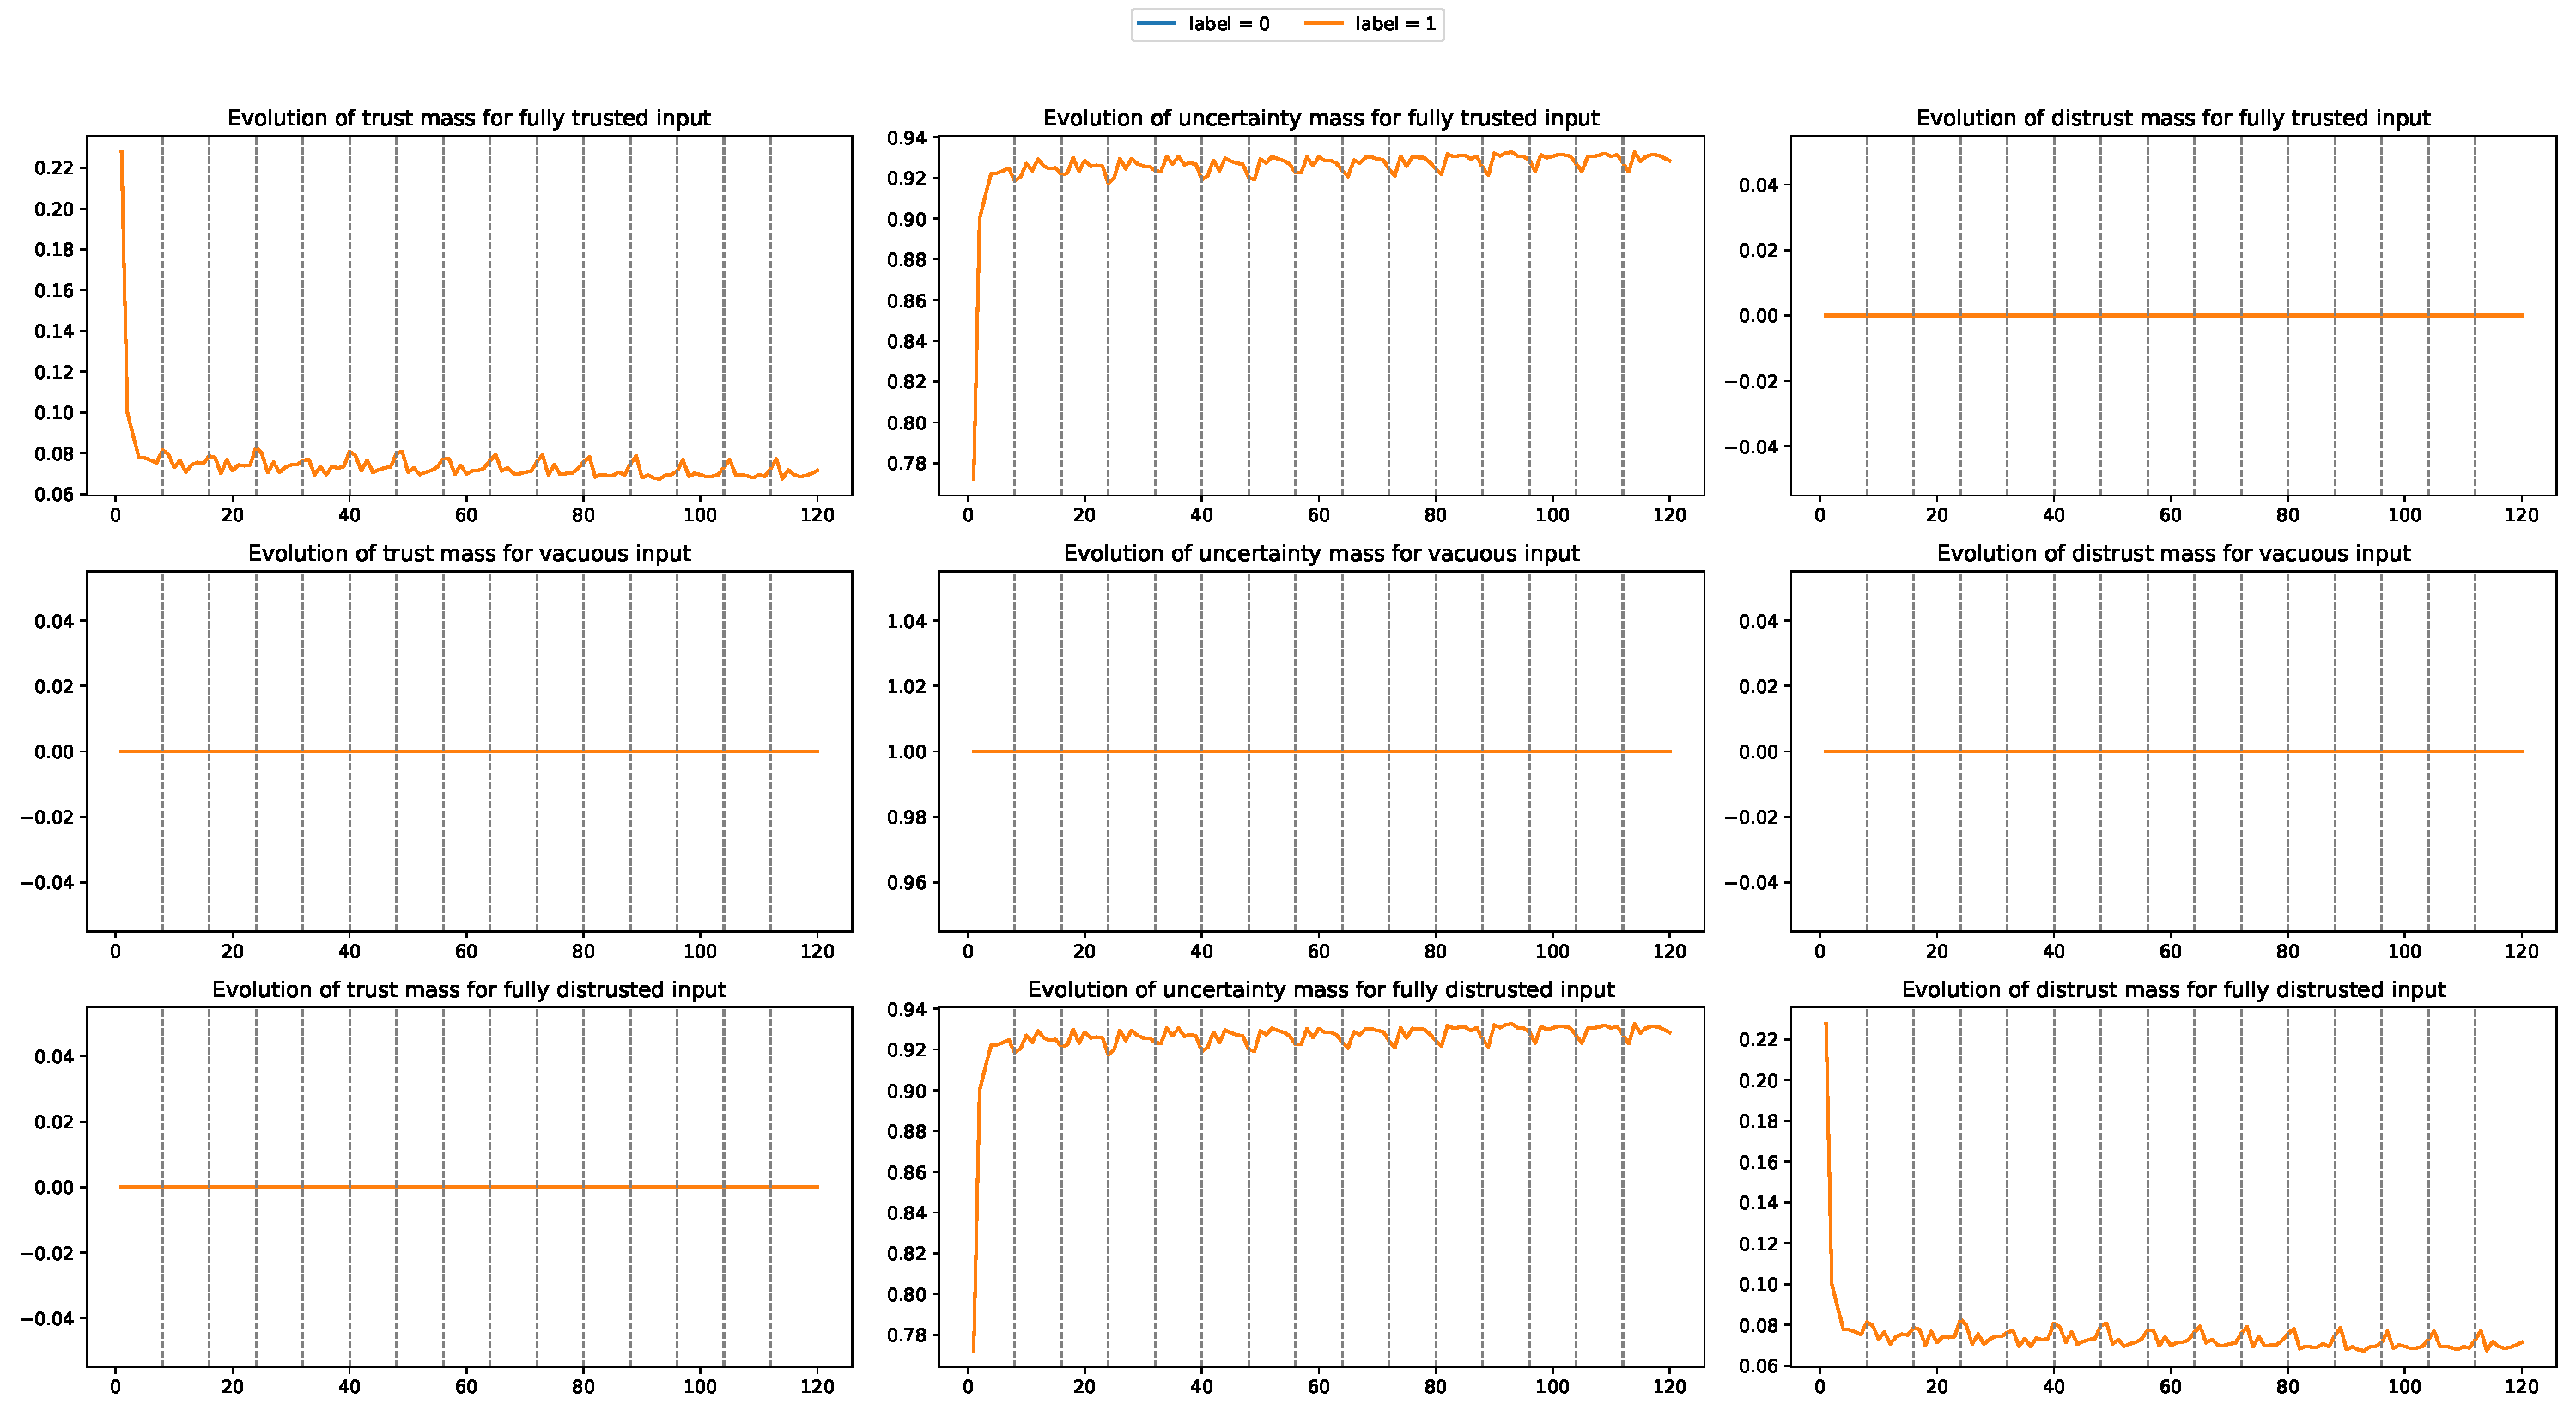
\includegraphics[width=0.8\textwidth]{latex/PTAS_Eval_cancer_16_trust_vacuous_eps_0.001_PathSize_None__plot_ptas.pdf}
\caption{cancer\_16\_trust\_vacuous, $\varepsilon$=0.001}
\end{figure}

\begin{figure}[htbp]
\centering
  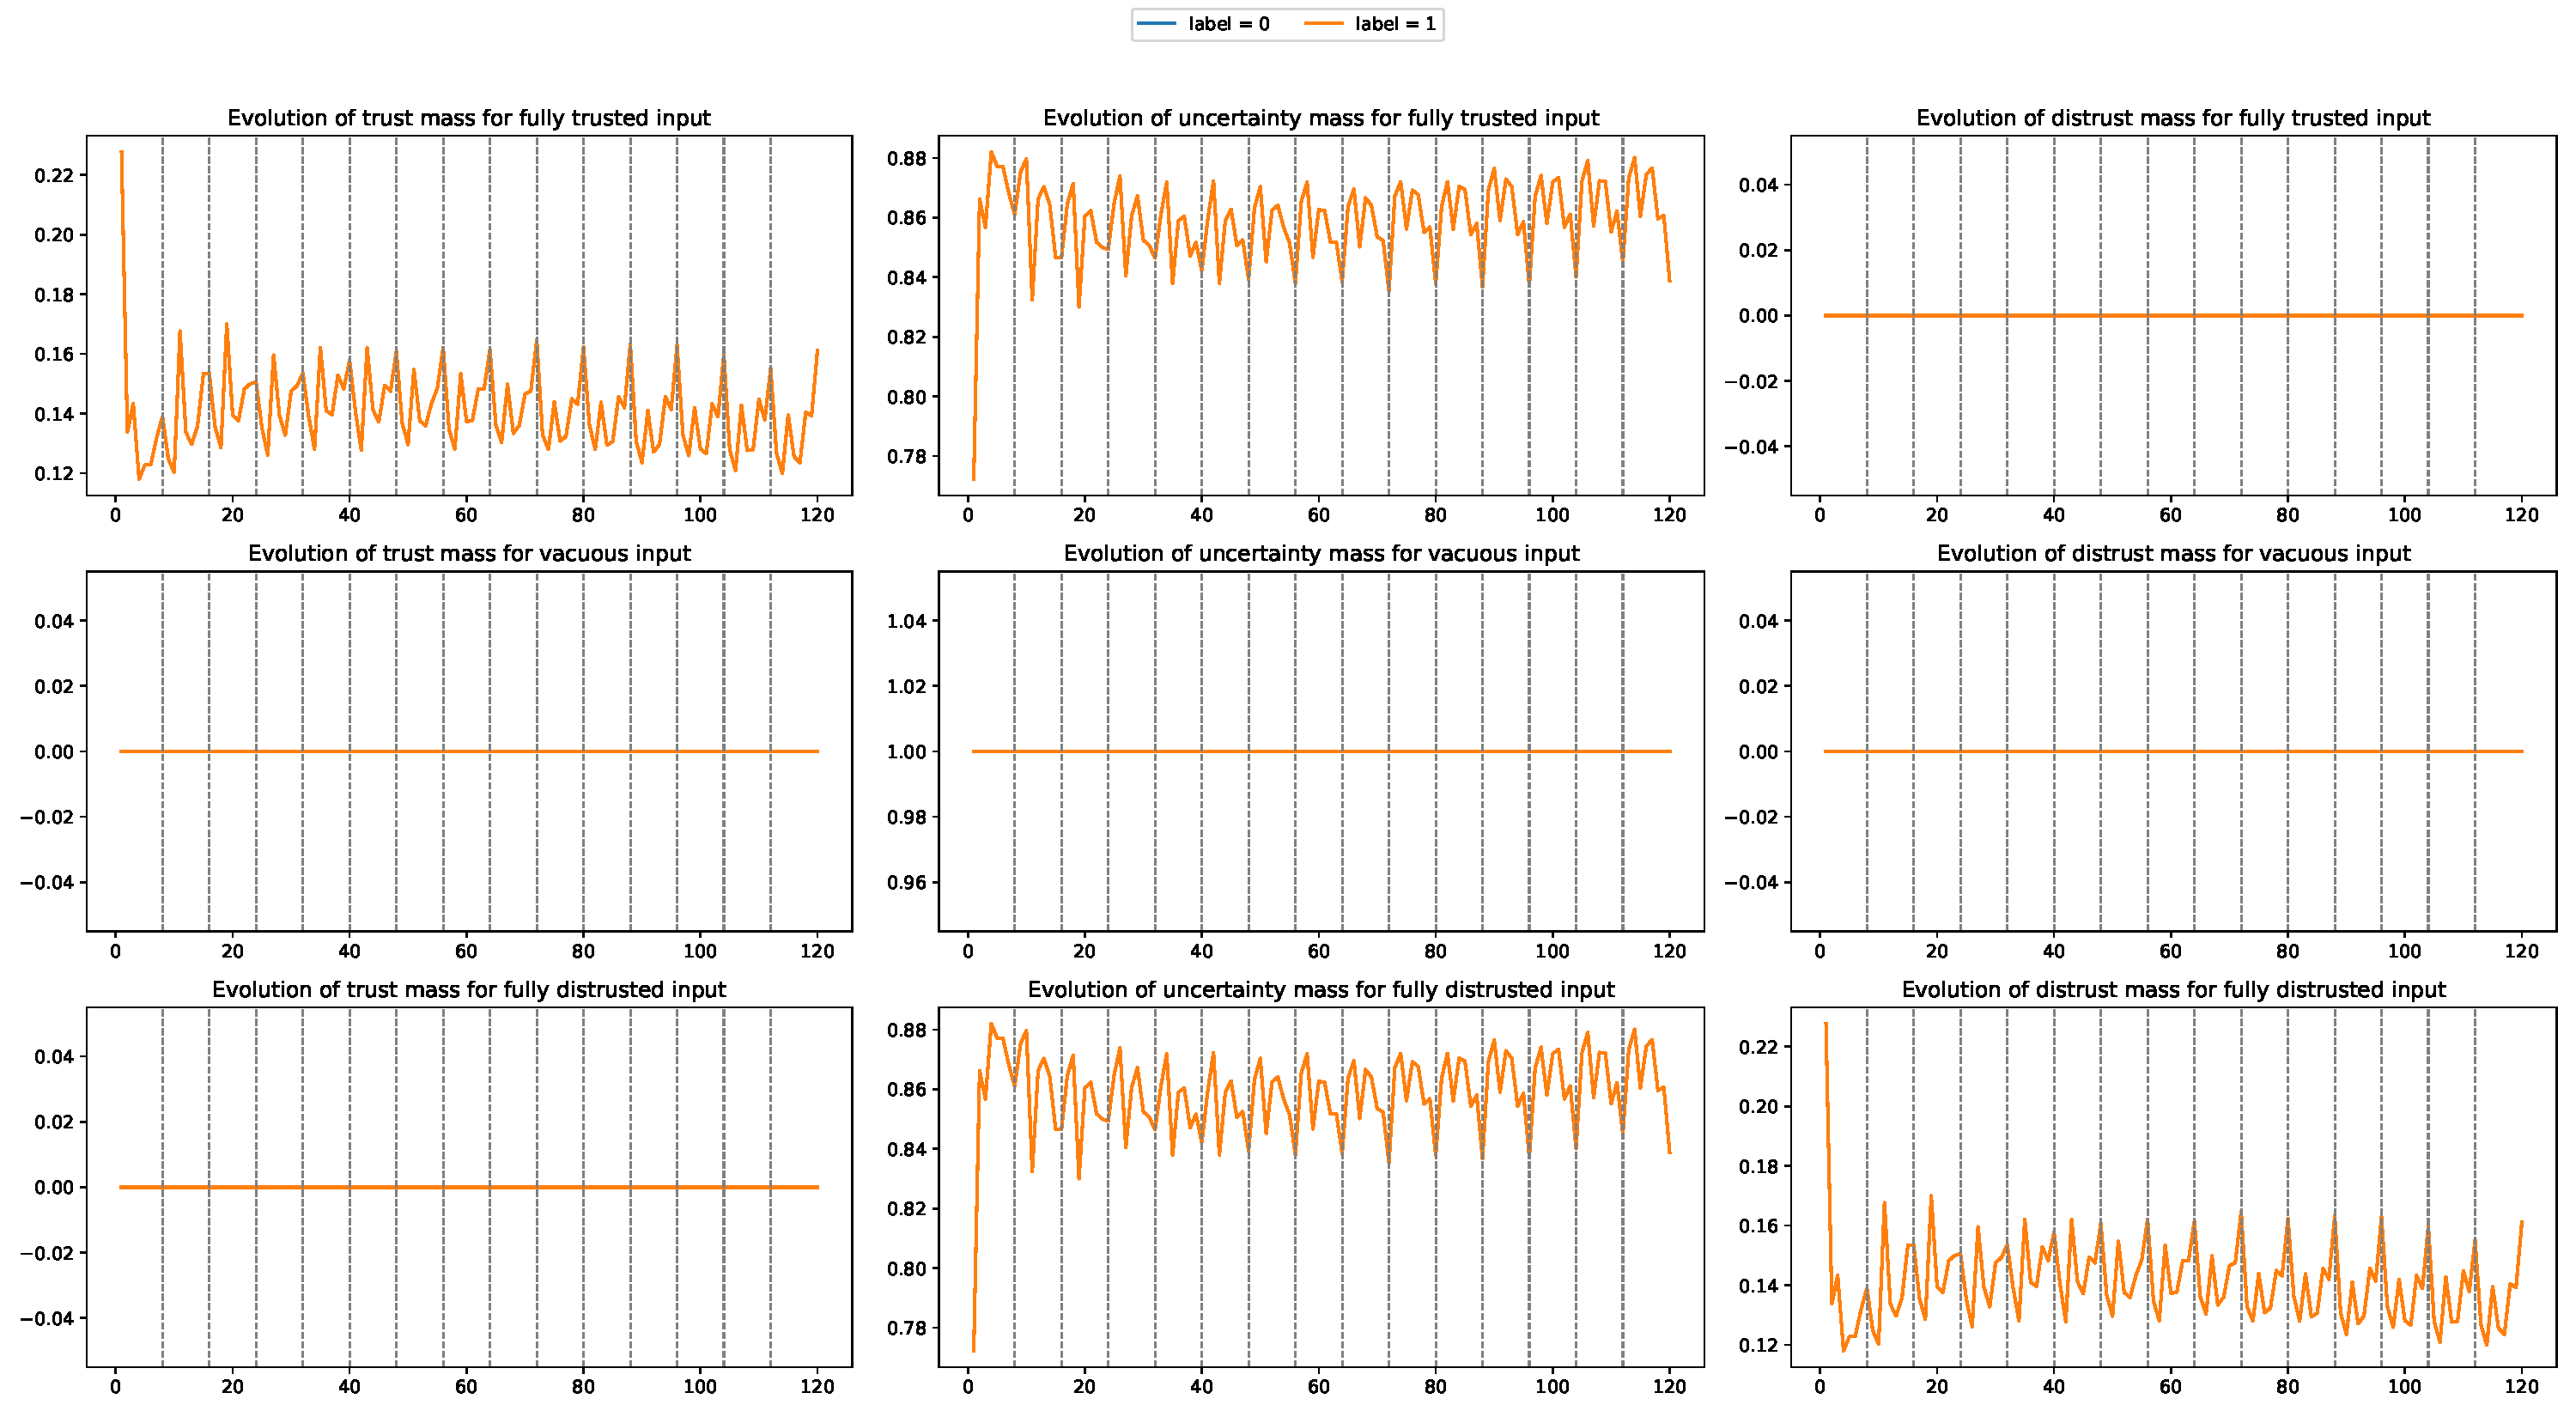
\includegraphics[width=0.8\textwidth]{latex/PTAS_Eval_cancer_16_trust_vacuous_eps_0.01_PathSize_None__plot_ptas.pdf}
\caption{cancer\_16\_trust\_vacuous, $\varepsilon$=0.01}
\end{figure}

\begin{figure}[htbp]
\centering
  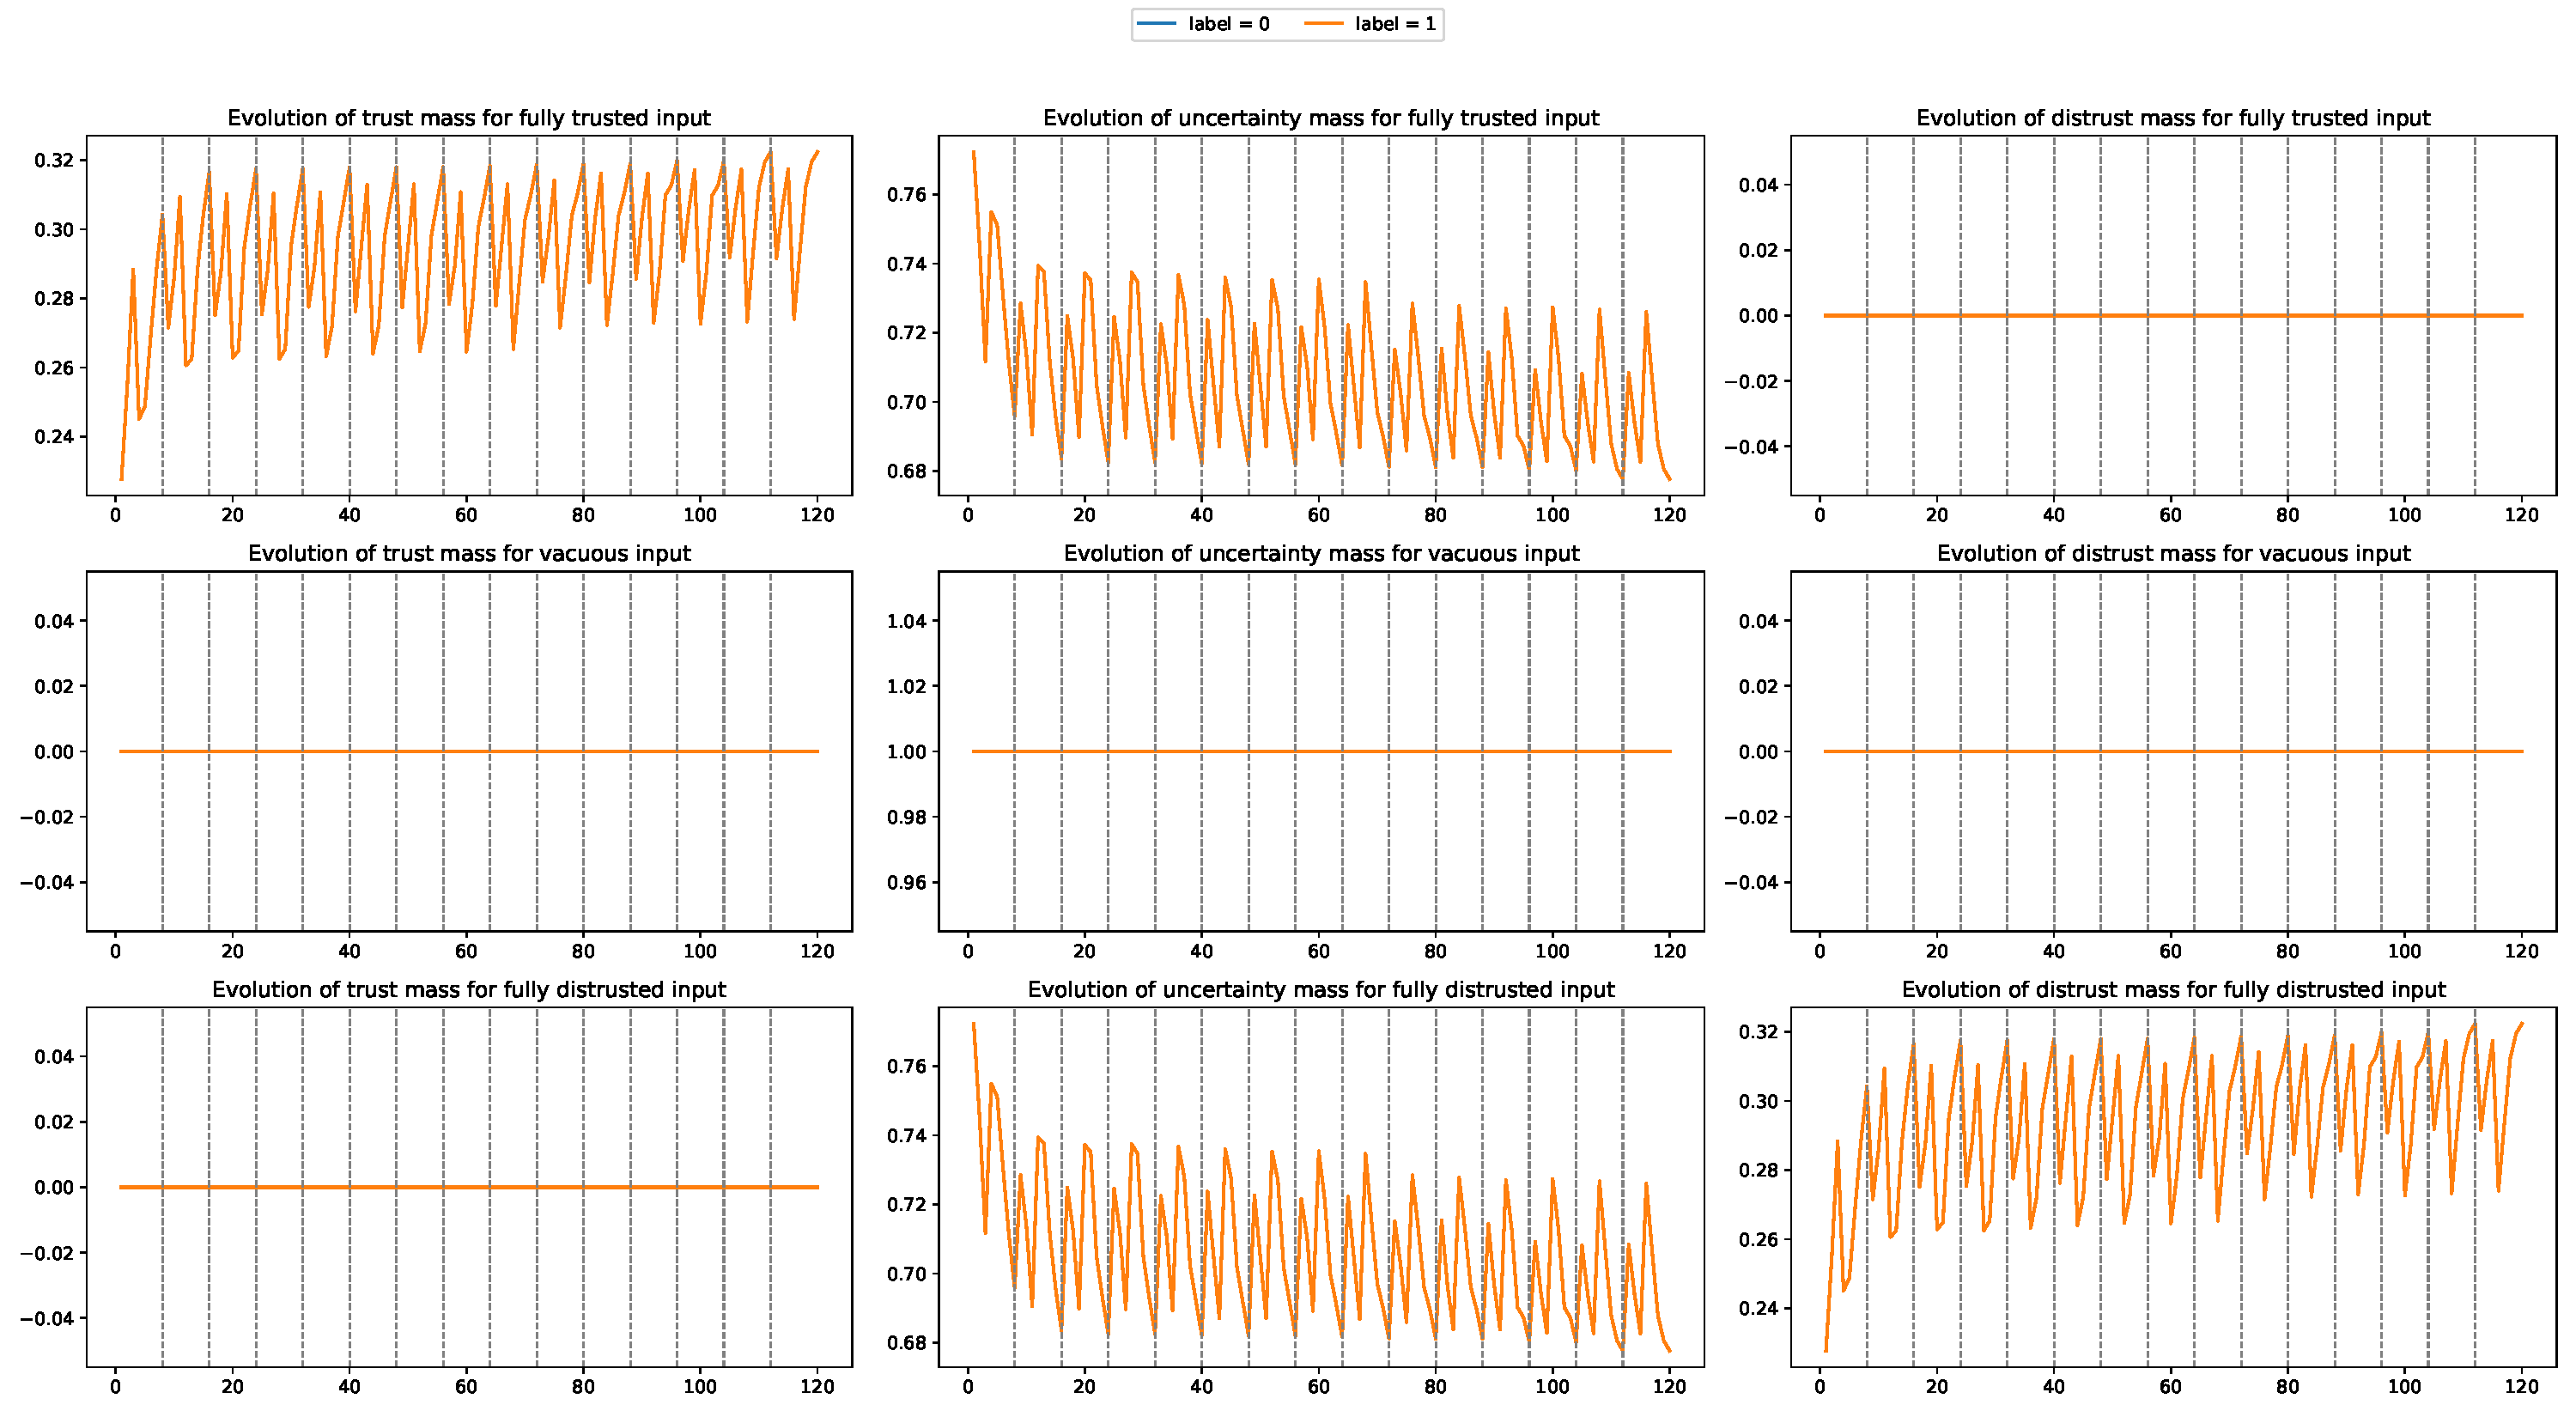
\includegraphics[width=0.8\textwidth]{latex/PTAS_Eval_cancer_16_trust_vacuous_eps_0.1_PathSize_None__plot_ptas.pdf}
\caption{cancer\_16\_trust\_vacuous, $\varepsilon$=0.1}
\end{figure}

\begin{figure}[htbp]
\centering
  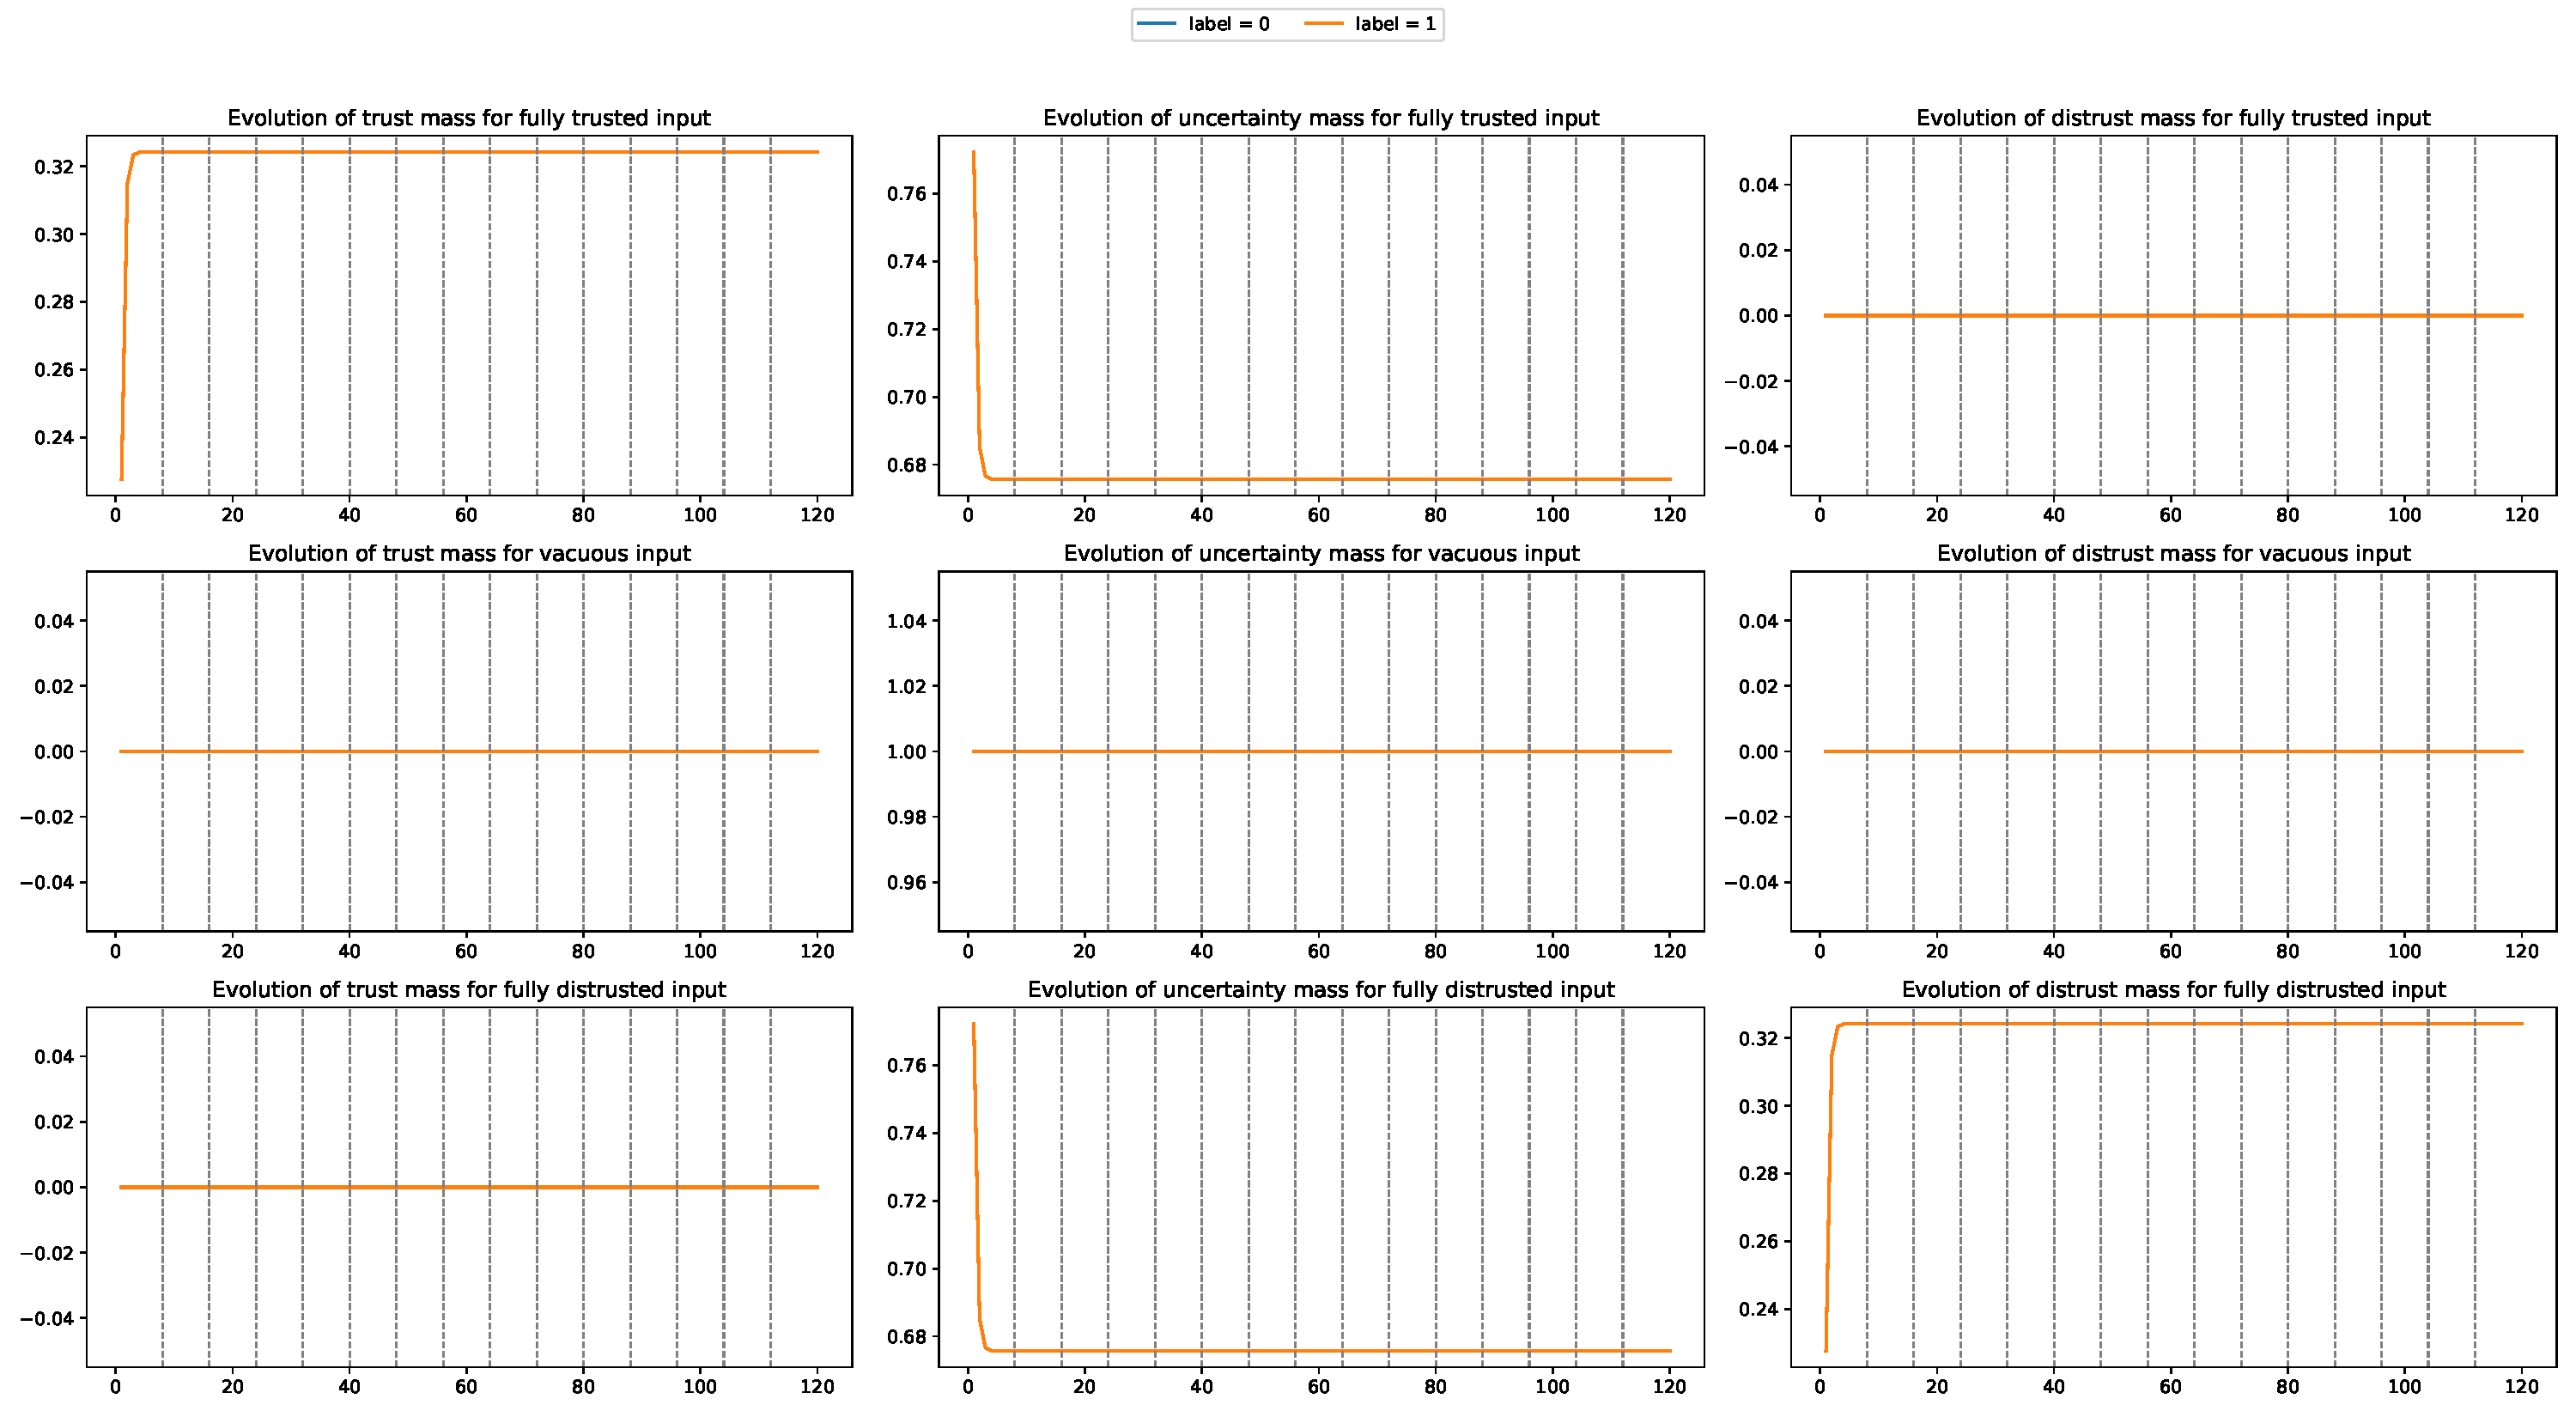
\includegraphics[width=0.8\textwidth]{latex/PTAS_Eval_cancer_16_trust_vacuous_eps_1_PathSize_None__plot_ptas.pdf}
\caption{cancer\_16\_trust\_vacuous, $\varepsilon$=1}
\end{figure}

\subsubsection{vacuous -- distrust}

\begin{figure}[htbp]
\centering
  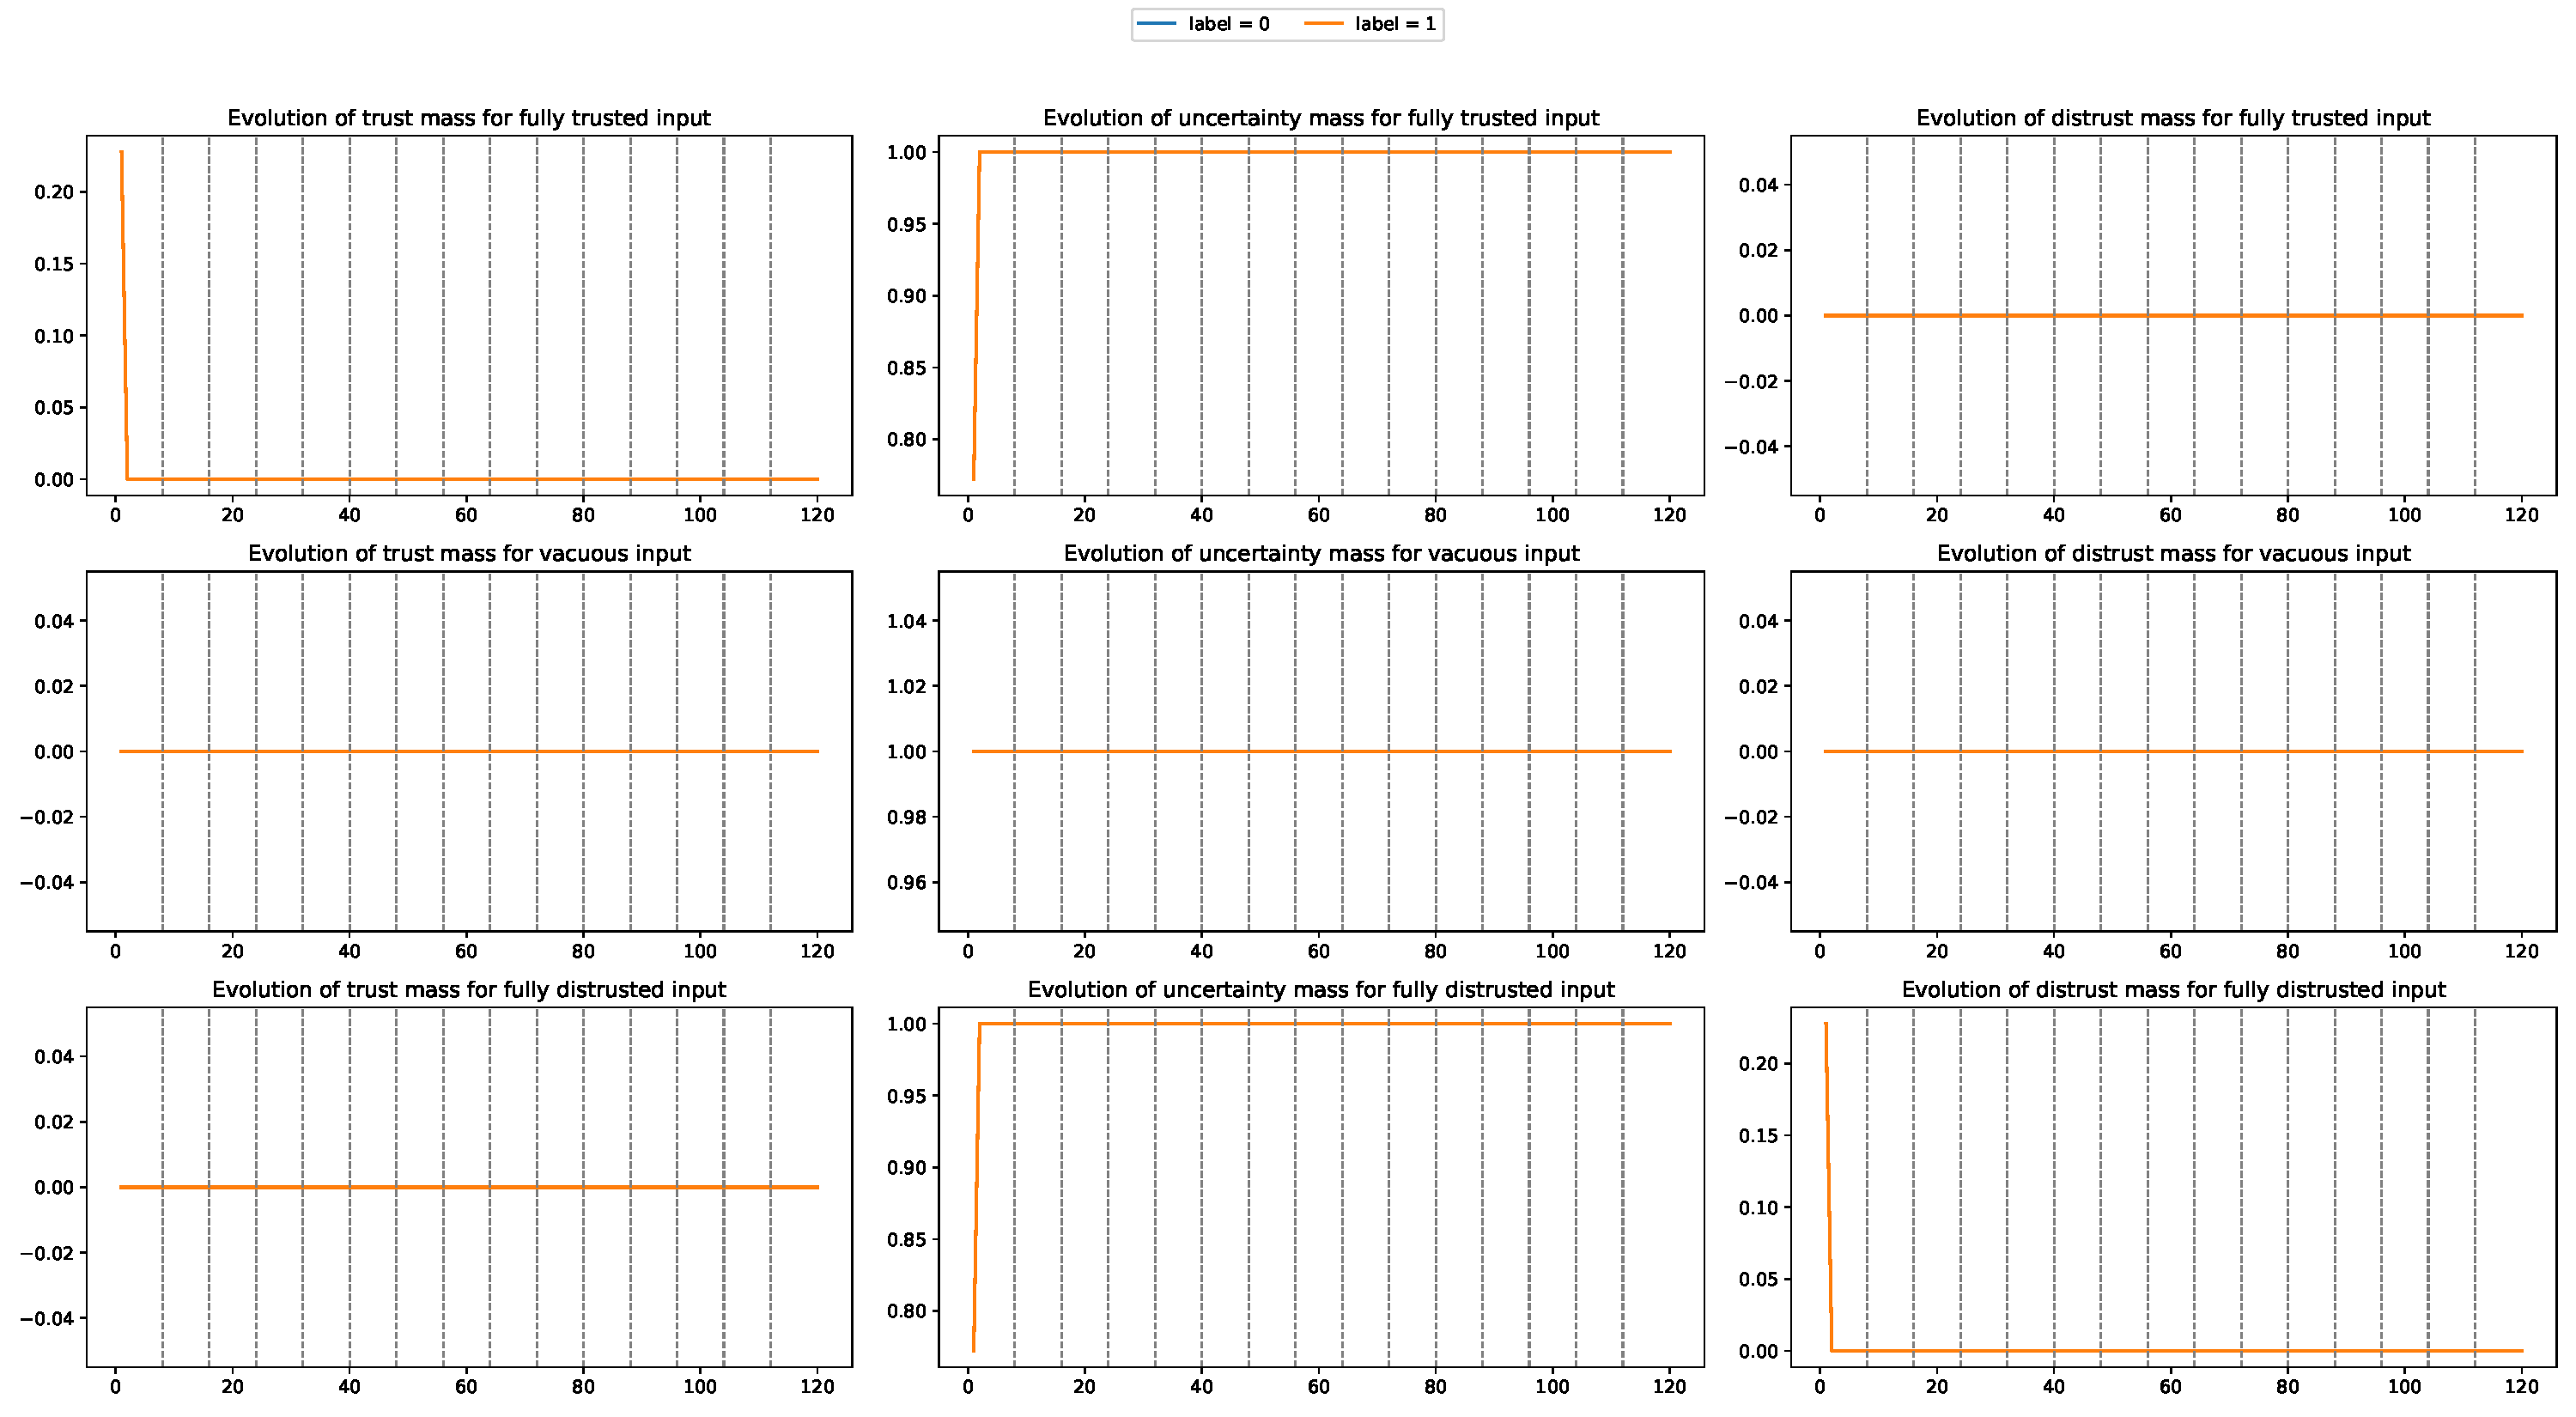
\includegraphics[width=0.8\textwidth]{latex/PTAS_Eval_cancer_16_vacuous_distrust_eps_0.001_PathSize_None__plot_ptas.pdf}
\caption{cancer\_16\_vacuous\_distrust, $\varepsilon$=0.001}
\end{figure}

\begin{figure}[htbp]
\centering
  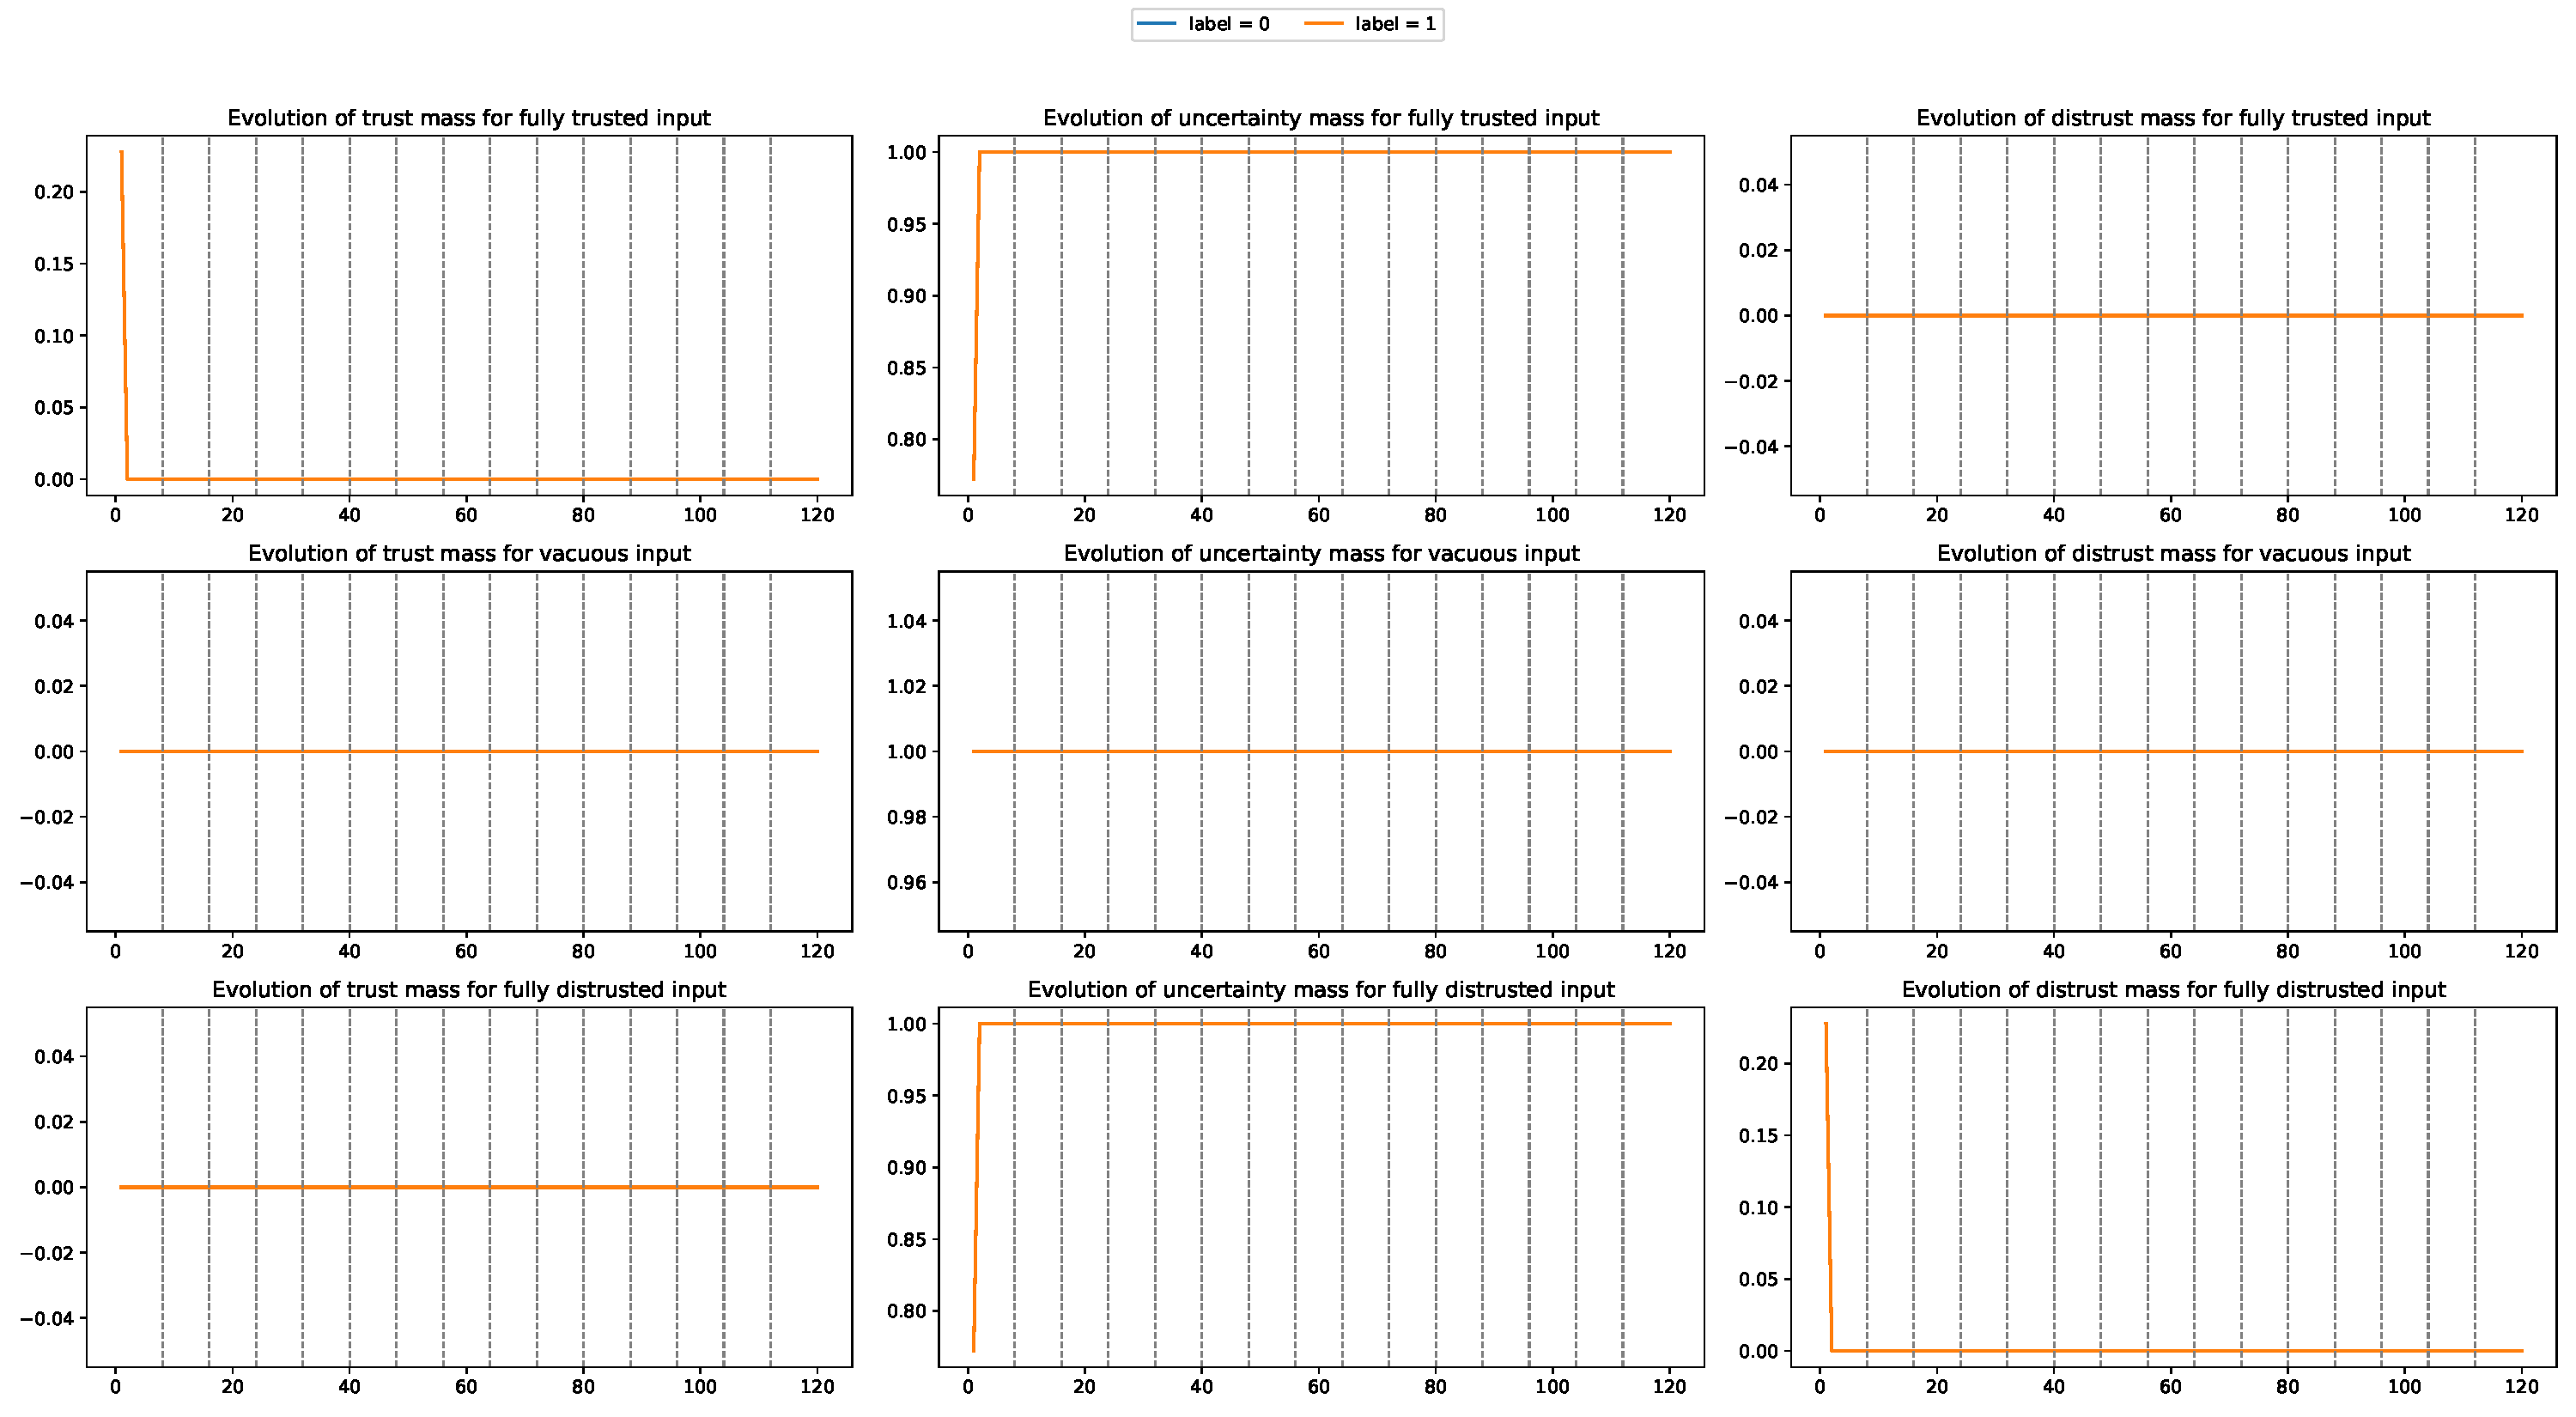
\includegraphics[width=0.8\textwidth]{latex/PTAS_Eval_cancer_16_vacuous_distrust_eps_0.01_PathSize_None__plot_ptas.pdf}
\caption{cancer\_16\_vacuous\_distrust, $\varepsilon$=0.01}
\end{figure}

\begin{figure}[htbp]
\centering
  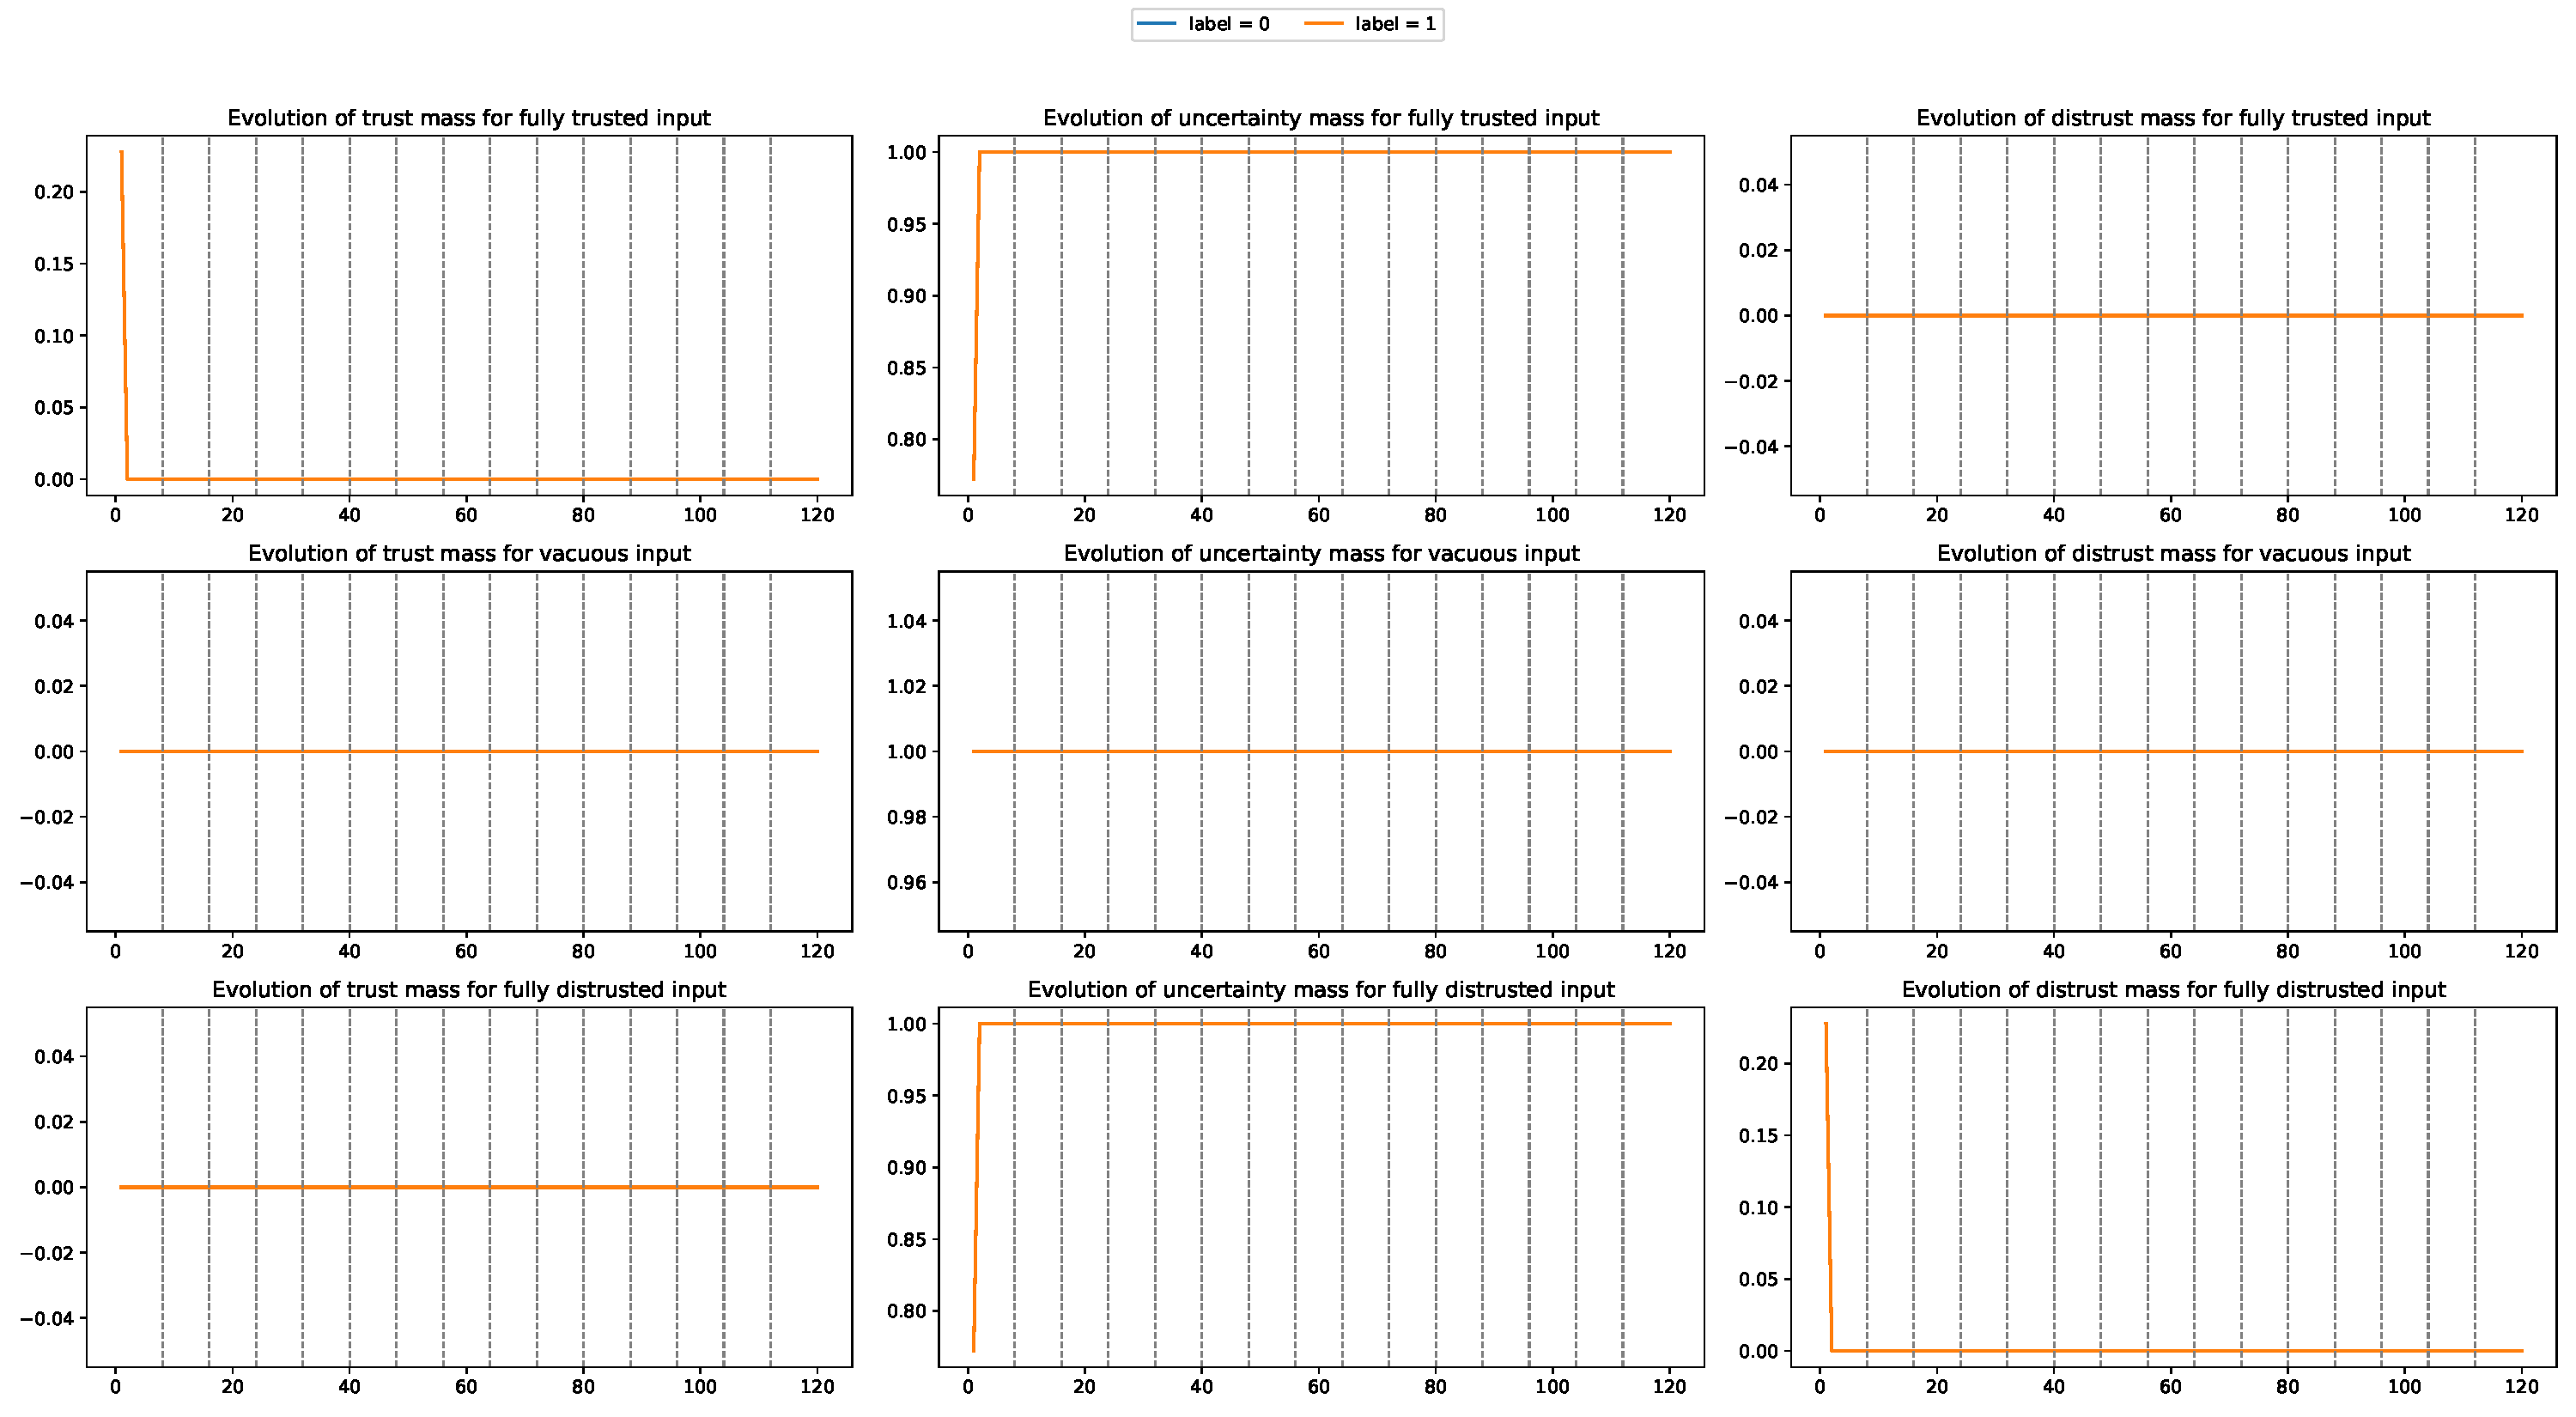
\includegraphics[width=0.8\textwidth]{latex/PTAS_Eval_cancer_16_vacuous_distrust_eps_0.1_PathSize_None__plot_ptas.pdf}
\caption{cancer\_16\_vacuous\_distrust, $\varepsilon$=0.1}
\end{figure}

\begin{figure}[htbp]
\centering
  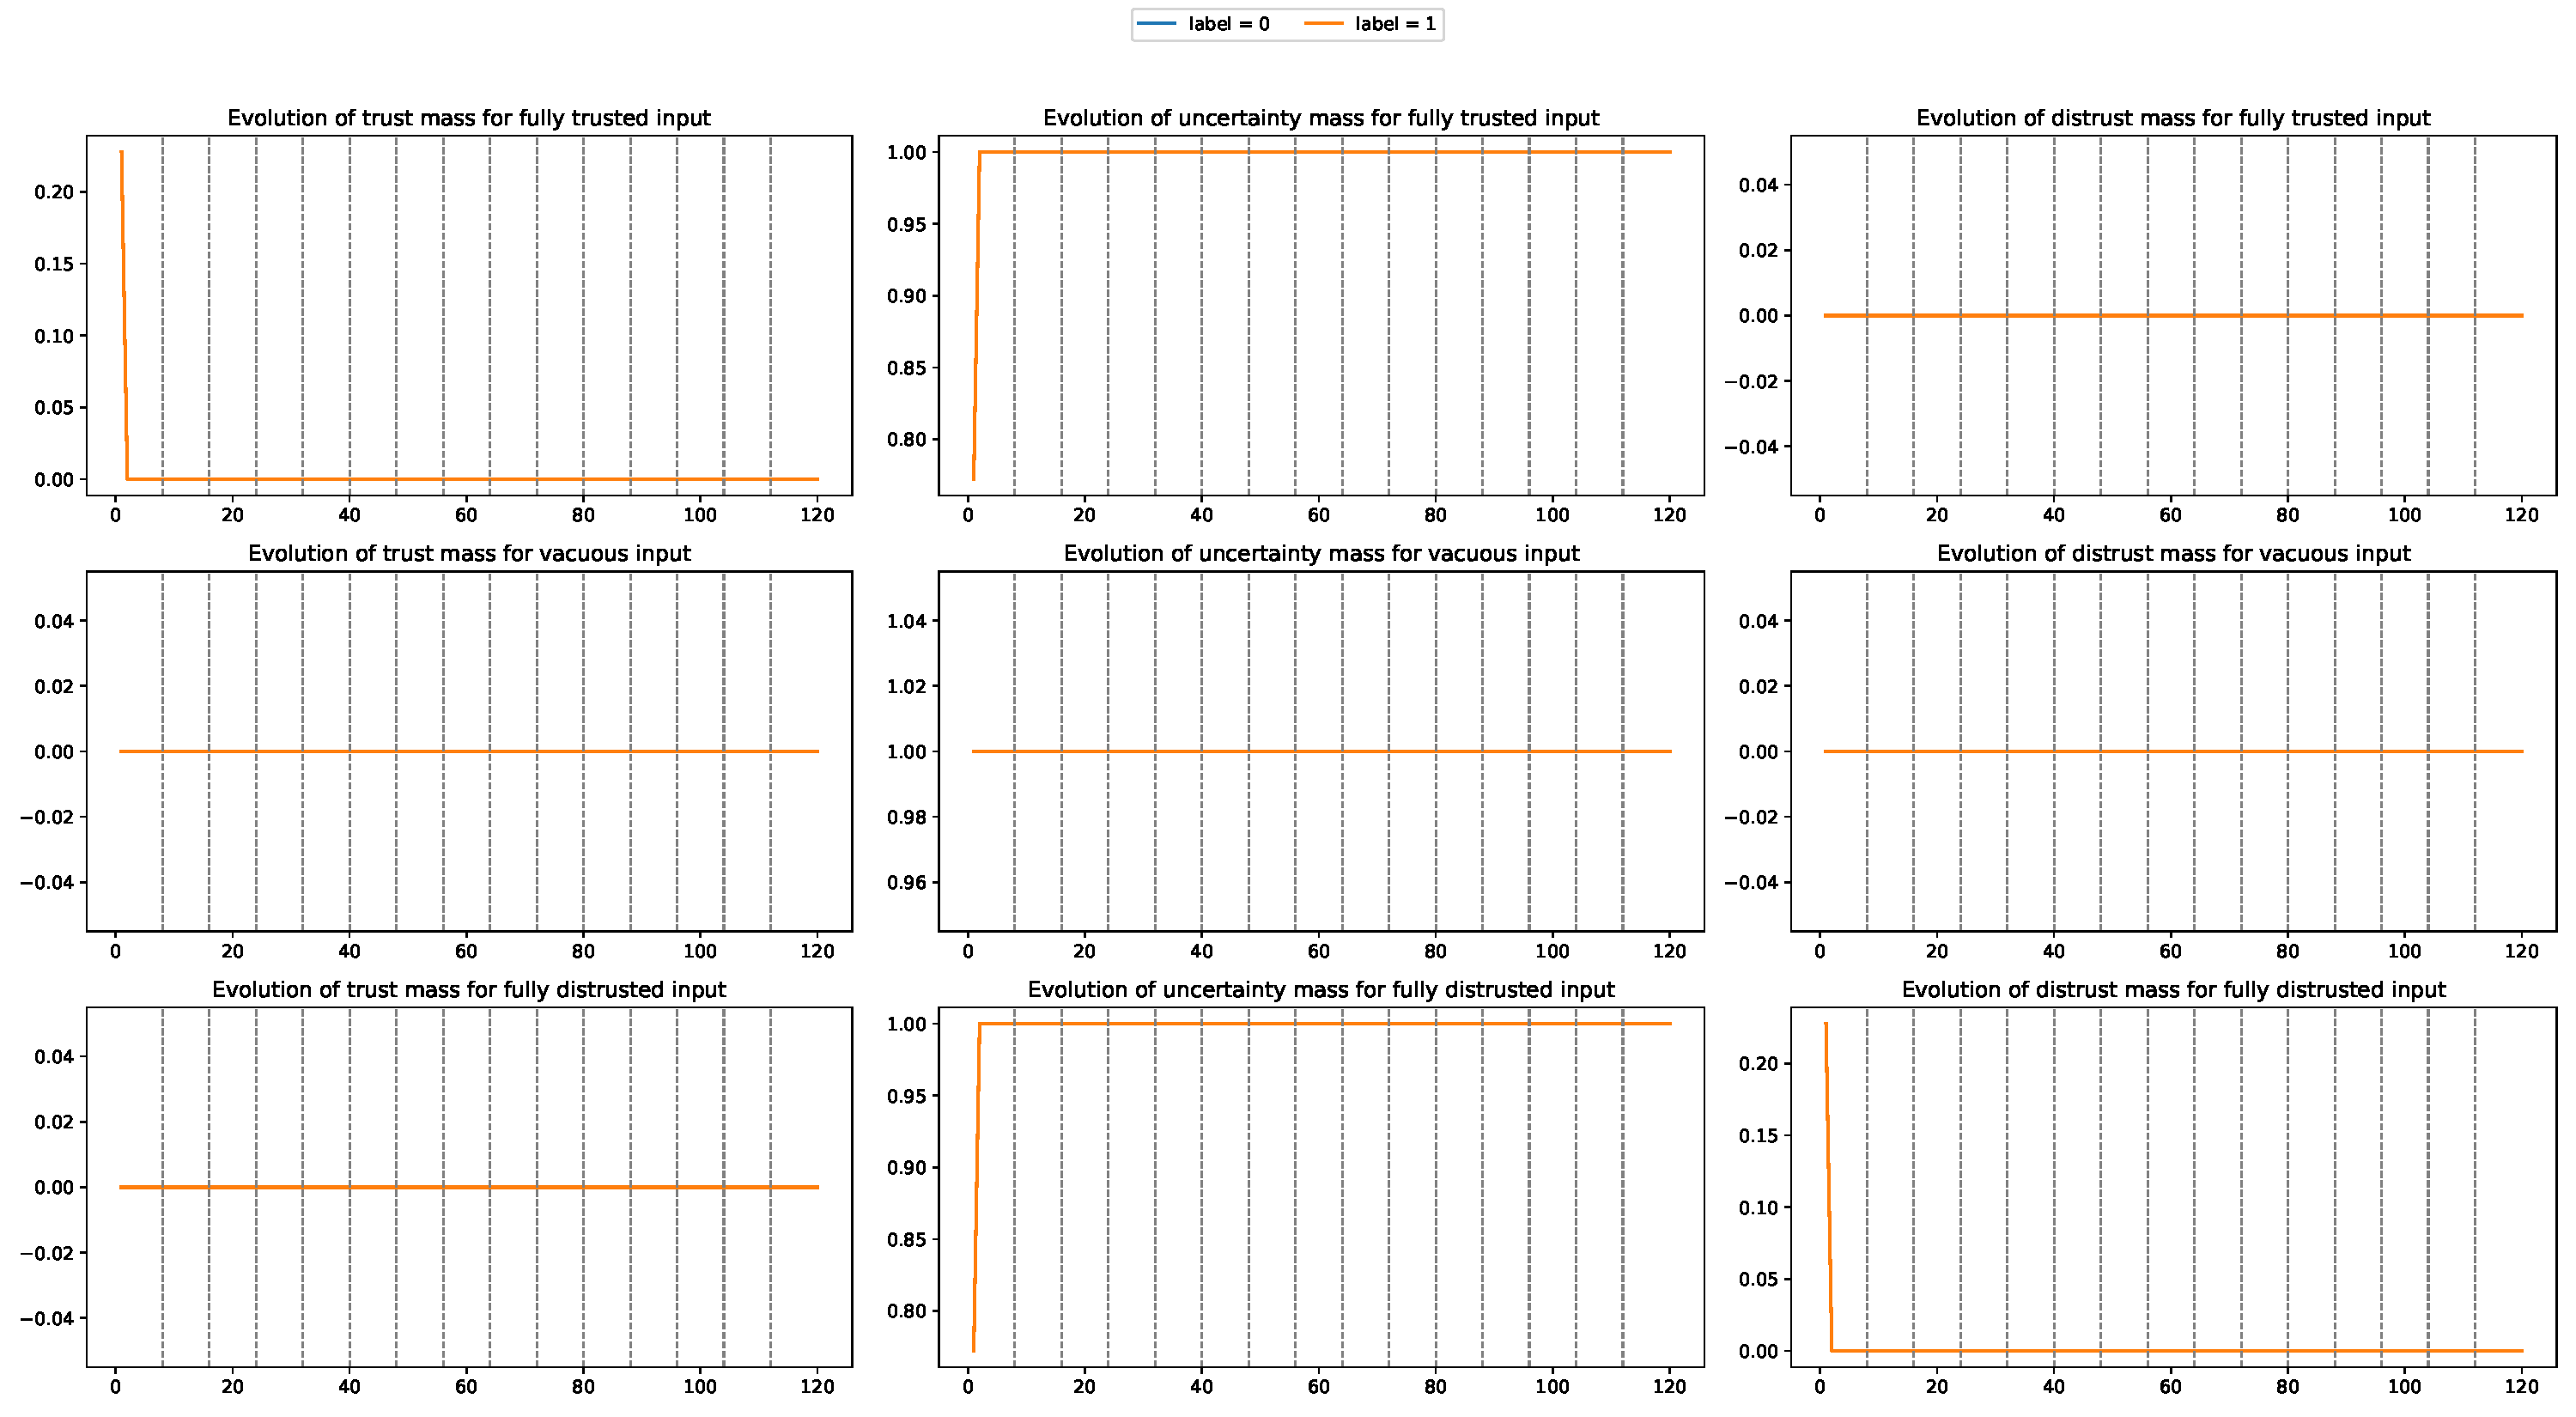
\includegraphics[width=0.8\textwidth]{latex/PTAS_Eval_cancer_16_vacuous_distrust_eps_1_PathSize_None__plot_ptas.pdf}
\caption{cancer\_16\_vacuous\_distrust, $\varepsilon$=1}
\end{figure}

\subsubsection{vacuous -- trust}

\begin{figure}[htbp]
\centering
  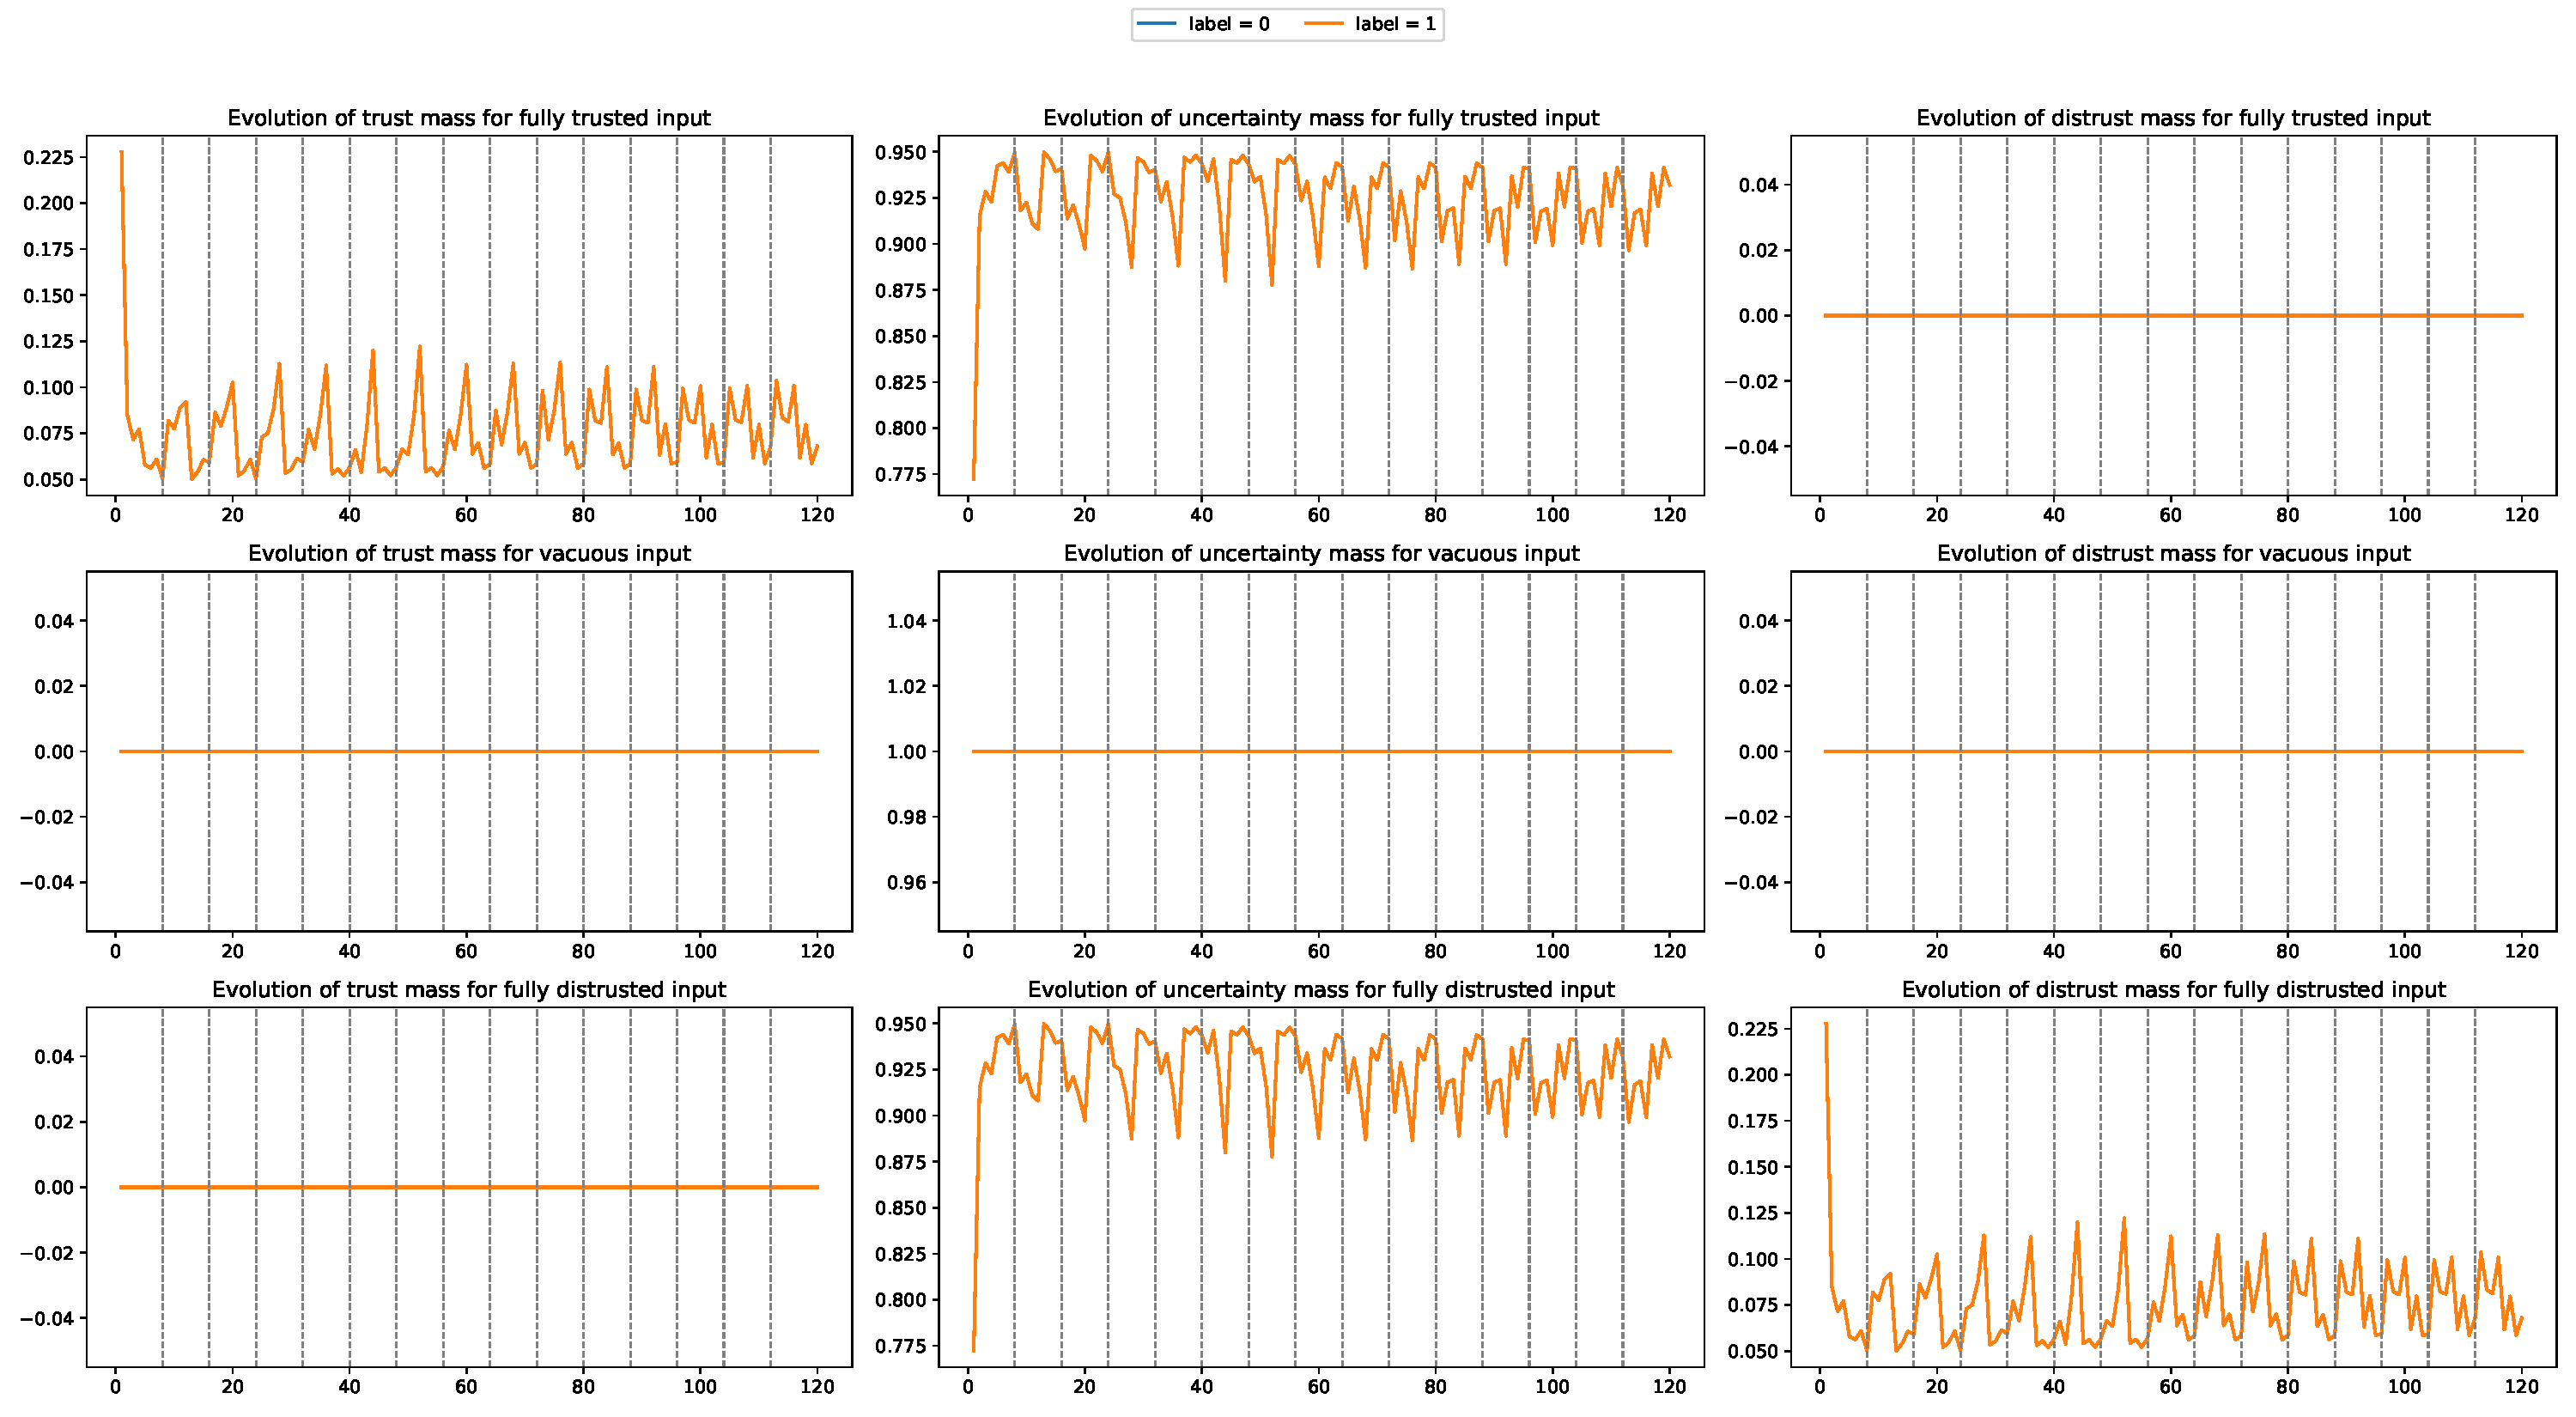
\includegraphics[width=0.8\textwidth]{latex/PTAS_Eval_cancer_16_vacuous_trust_eps_0.001_PathSize_None__plot_ptas.pdf}
\caption{cancer\_16\_vacuous\_trust, $\varepsilon$=0.001}
\end{figure}

\begin{figure}[htbp]
\centering
  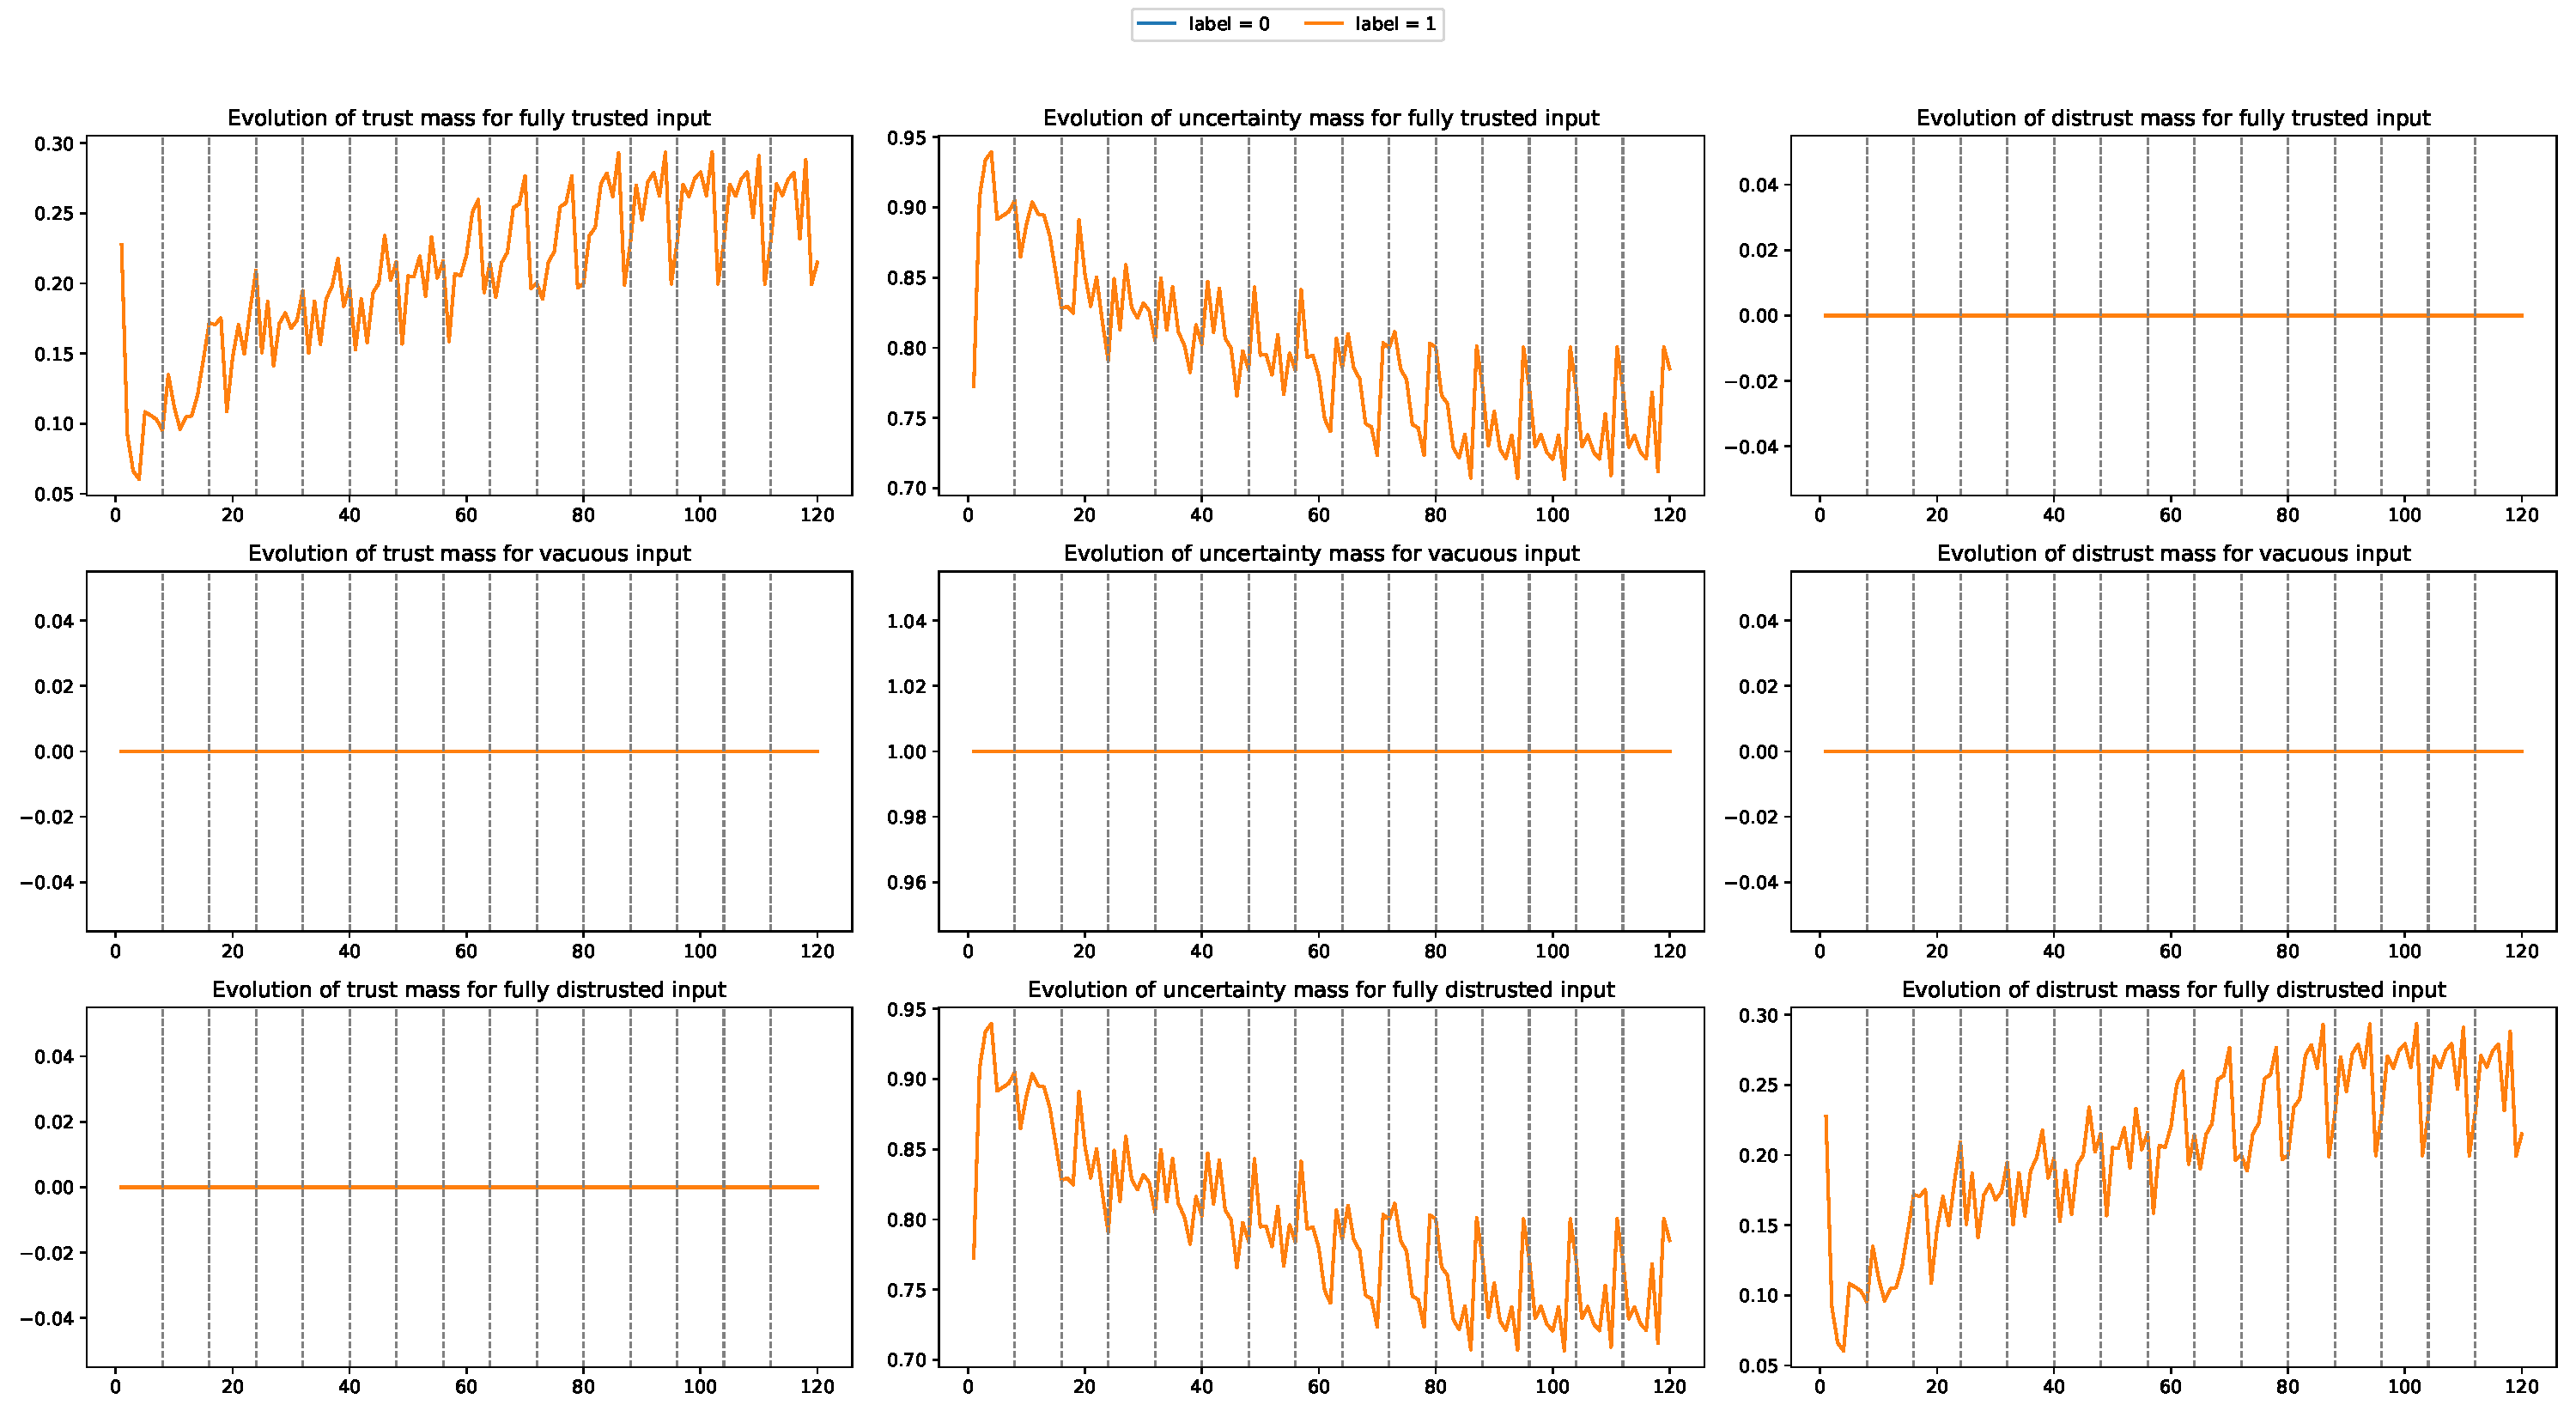
\includegraphics[width=0.8\textwidth]{latex/PTAS_Eval_cancer_16_vacuous_trust_eps_0.01_PathSize_None__plot_ptas.pdf}
\caption{cancer\_16\_vacuous\_trust, $\varepsilon$=0.01}
\end{figure}

\begin{figure}[htbp]
\centering
  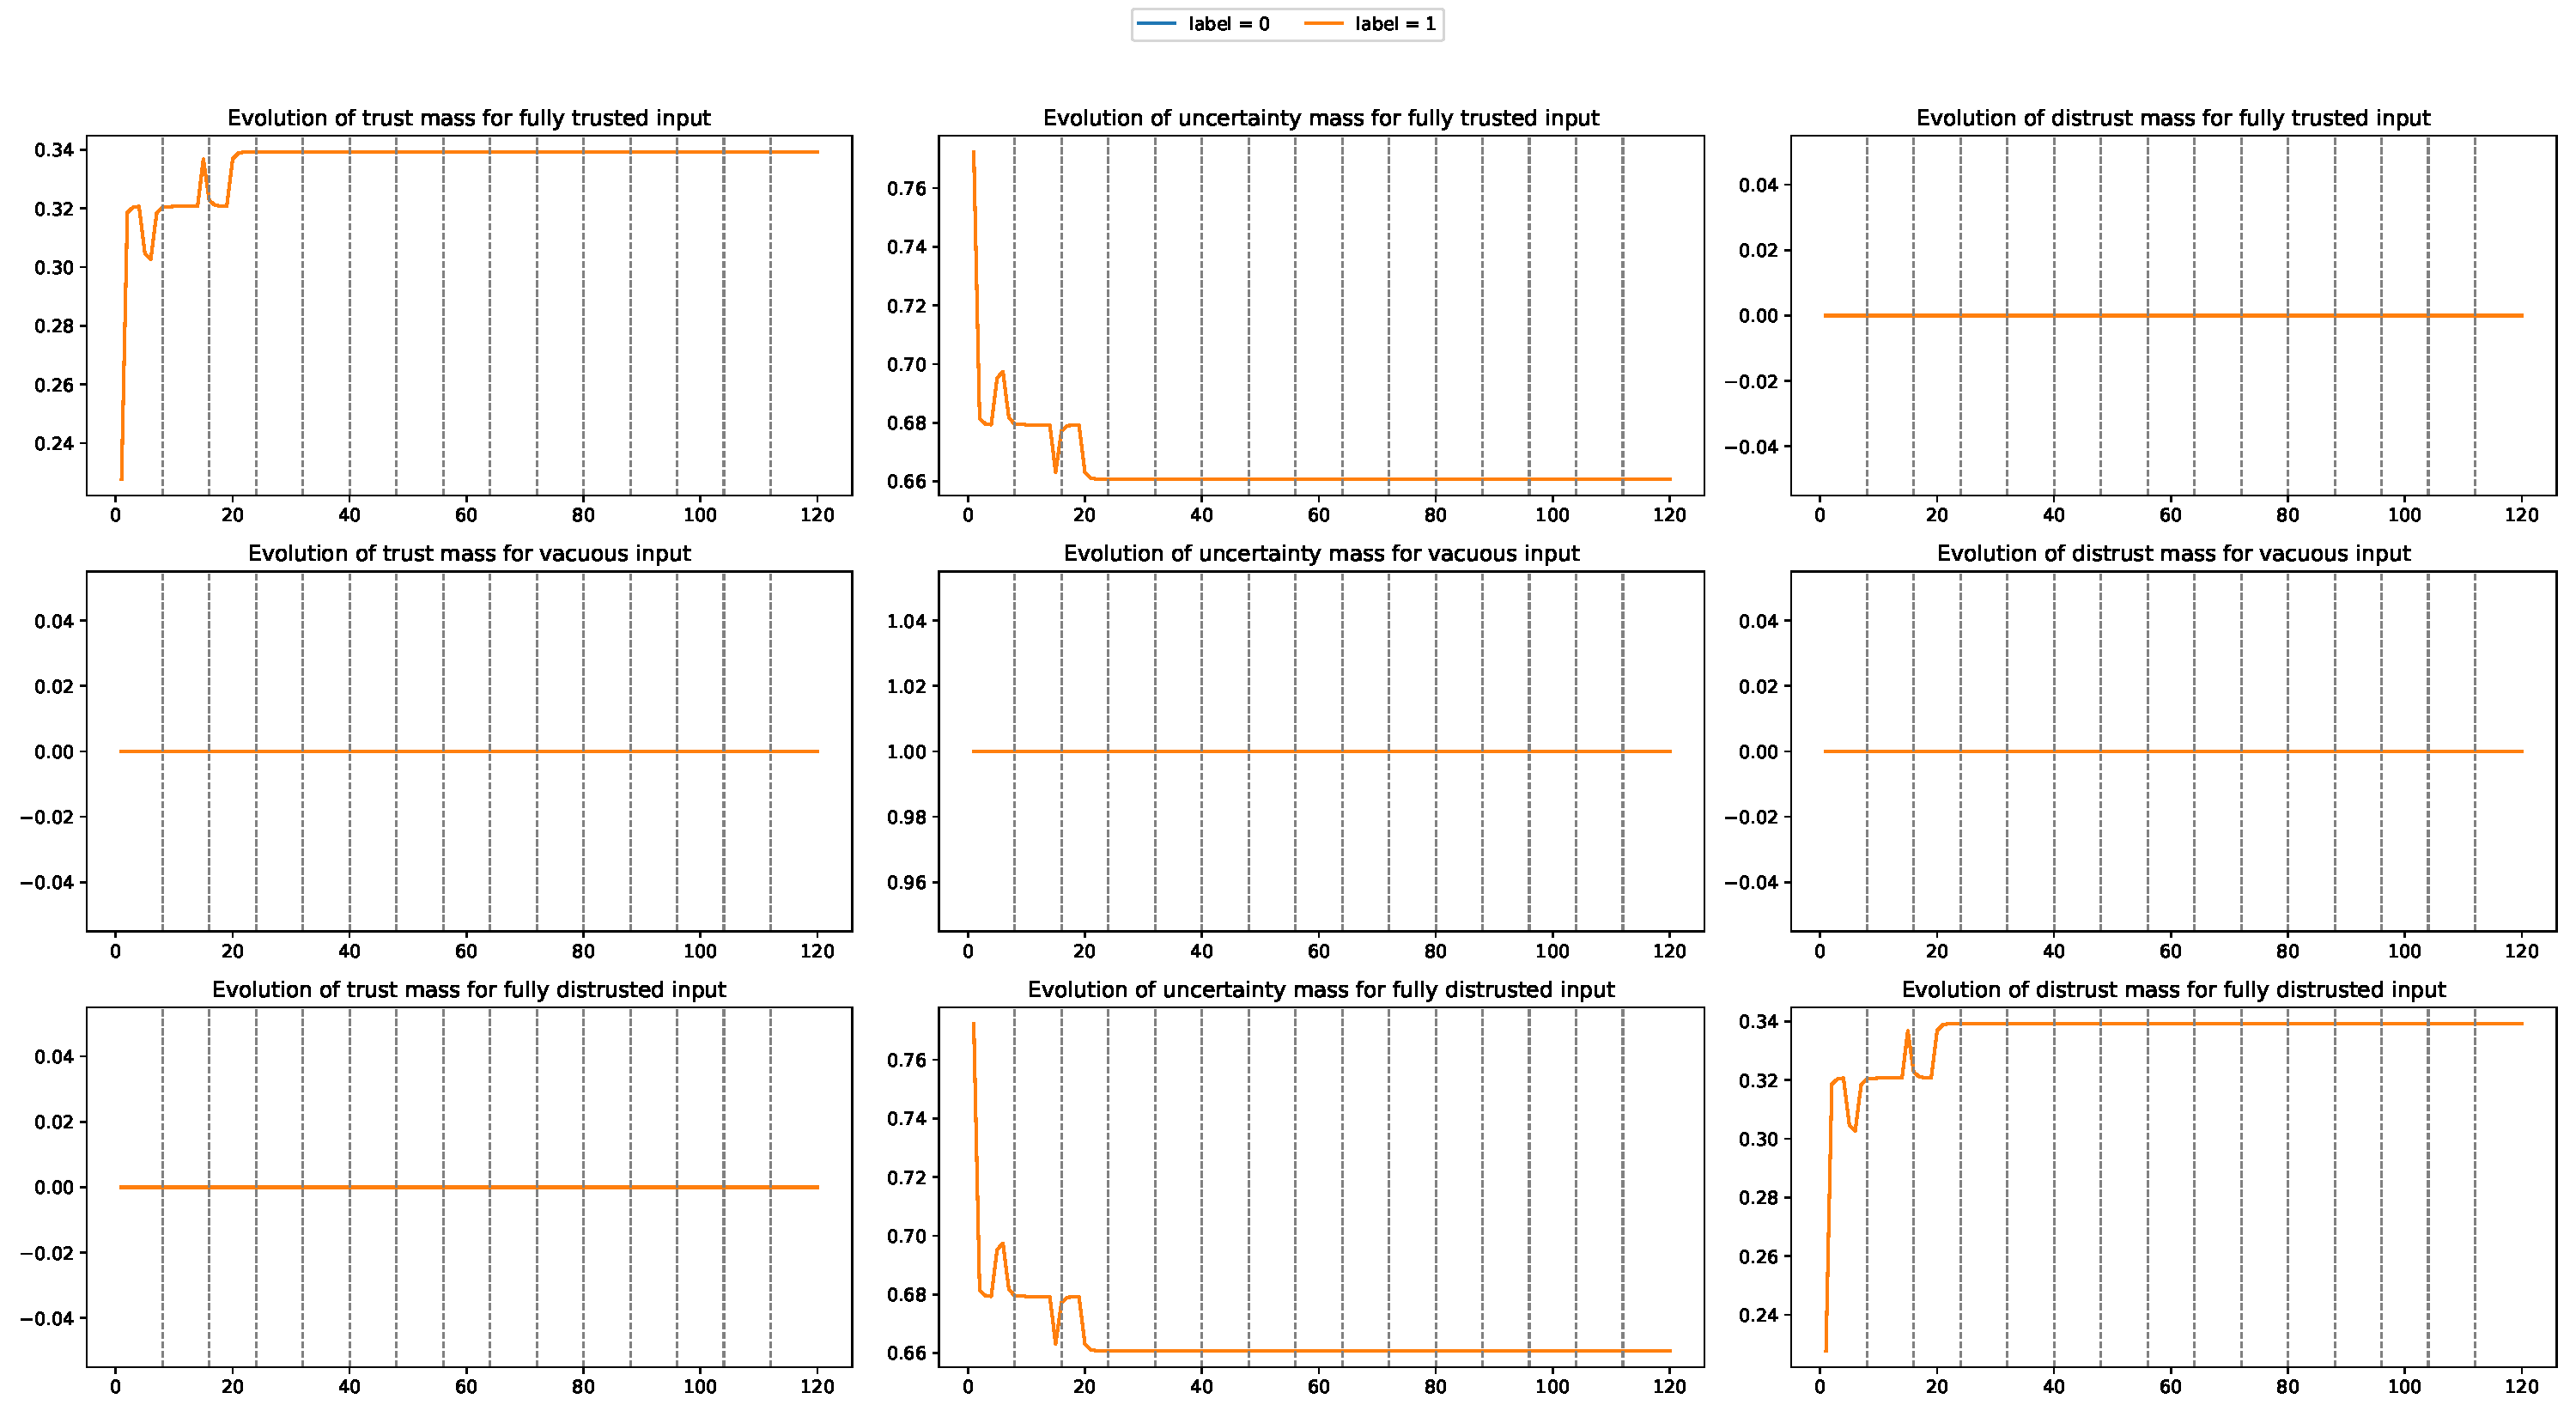
\includegraphics[width=0.8\textwidth]{latex/PTAS_Eval_cancer_16_vacuous_trust_eps_0.1_PathSize_None__plot_ptas.pdf}
\caption{cancer\_16\_vacuous\_trust, $\varepsilon$=0.1}
\end{figure}

\begin{figure}[htbp]
\centering
  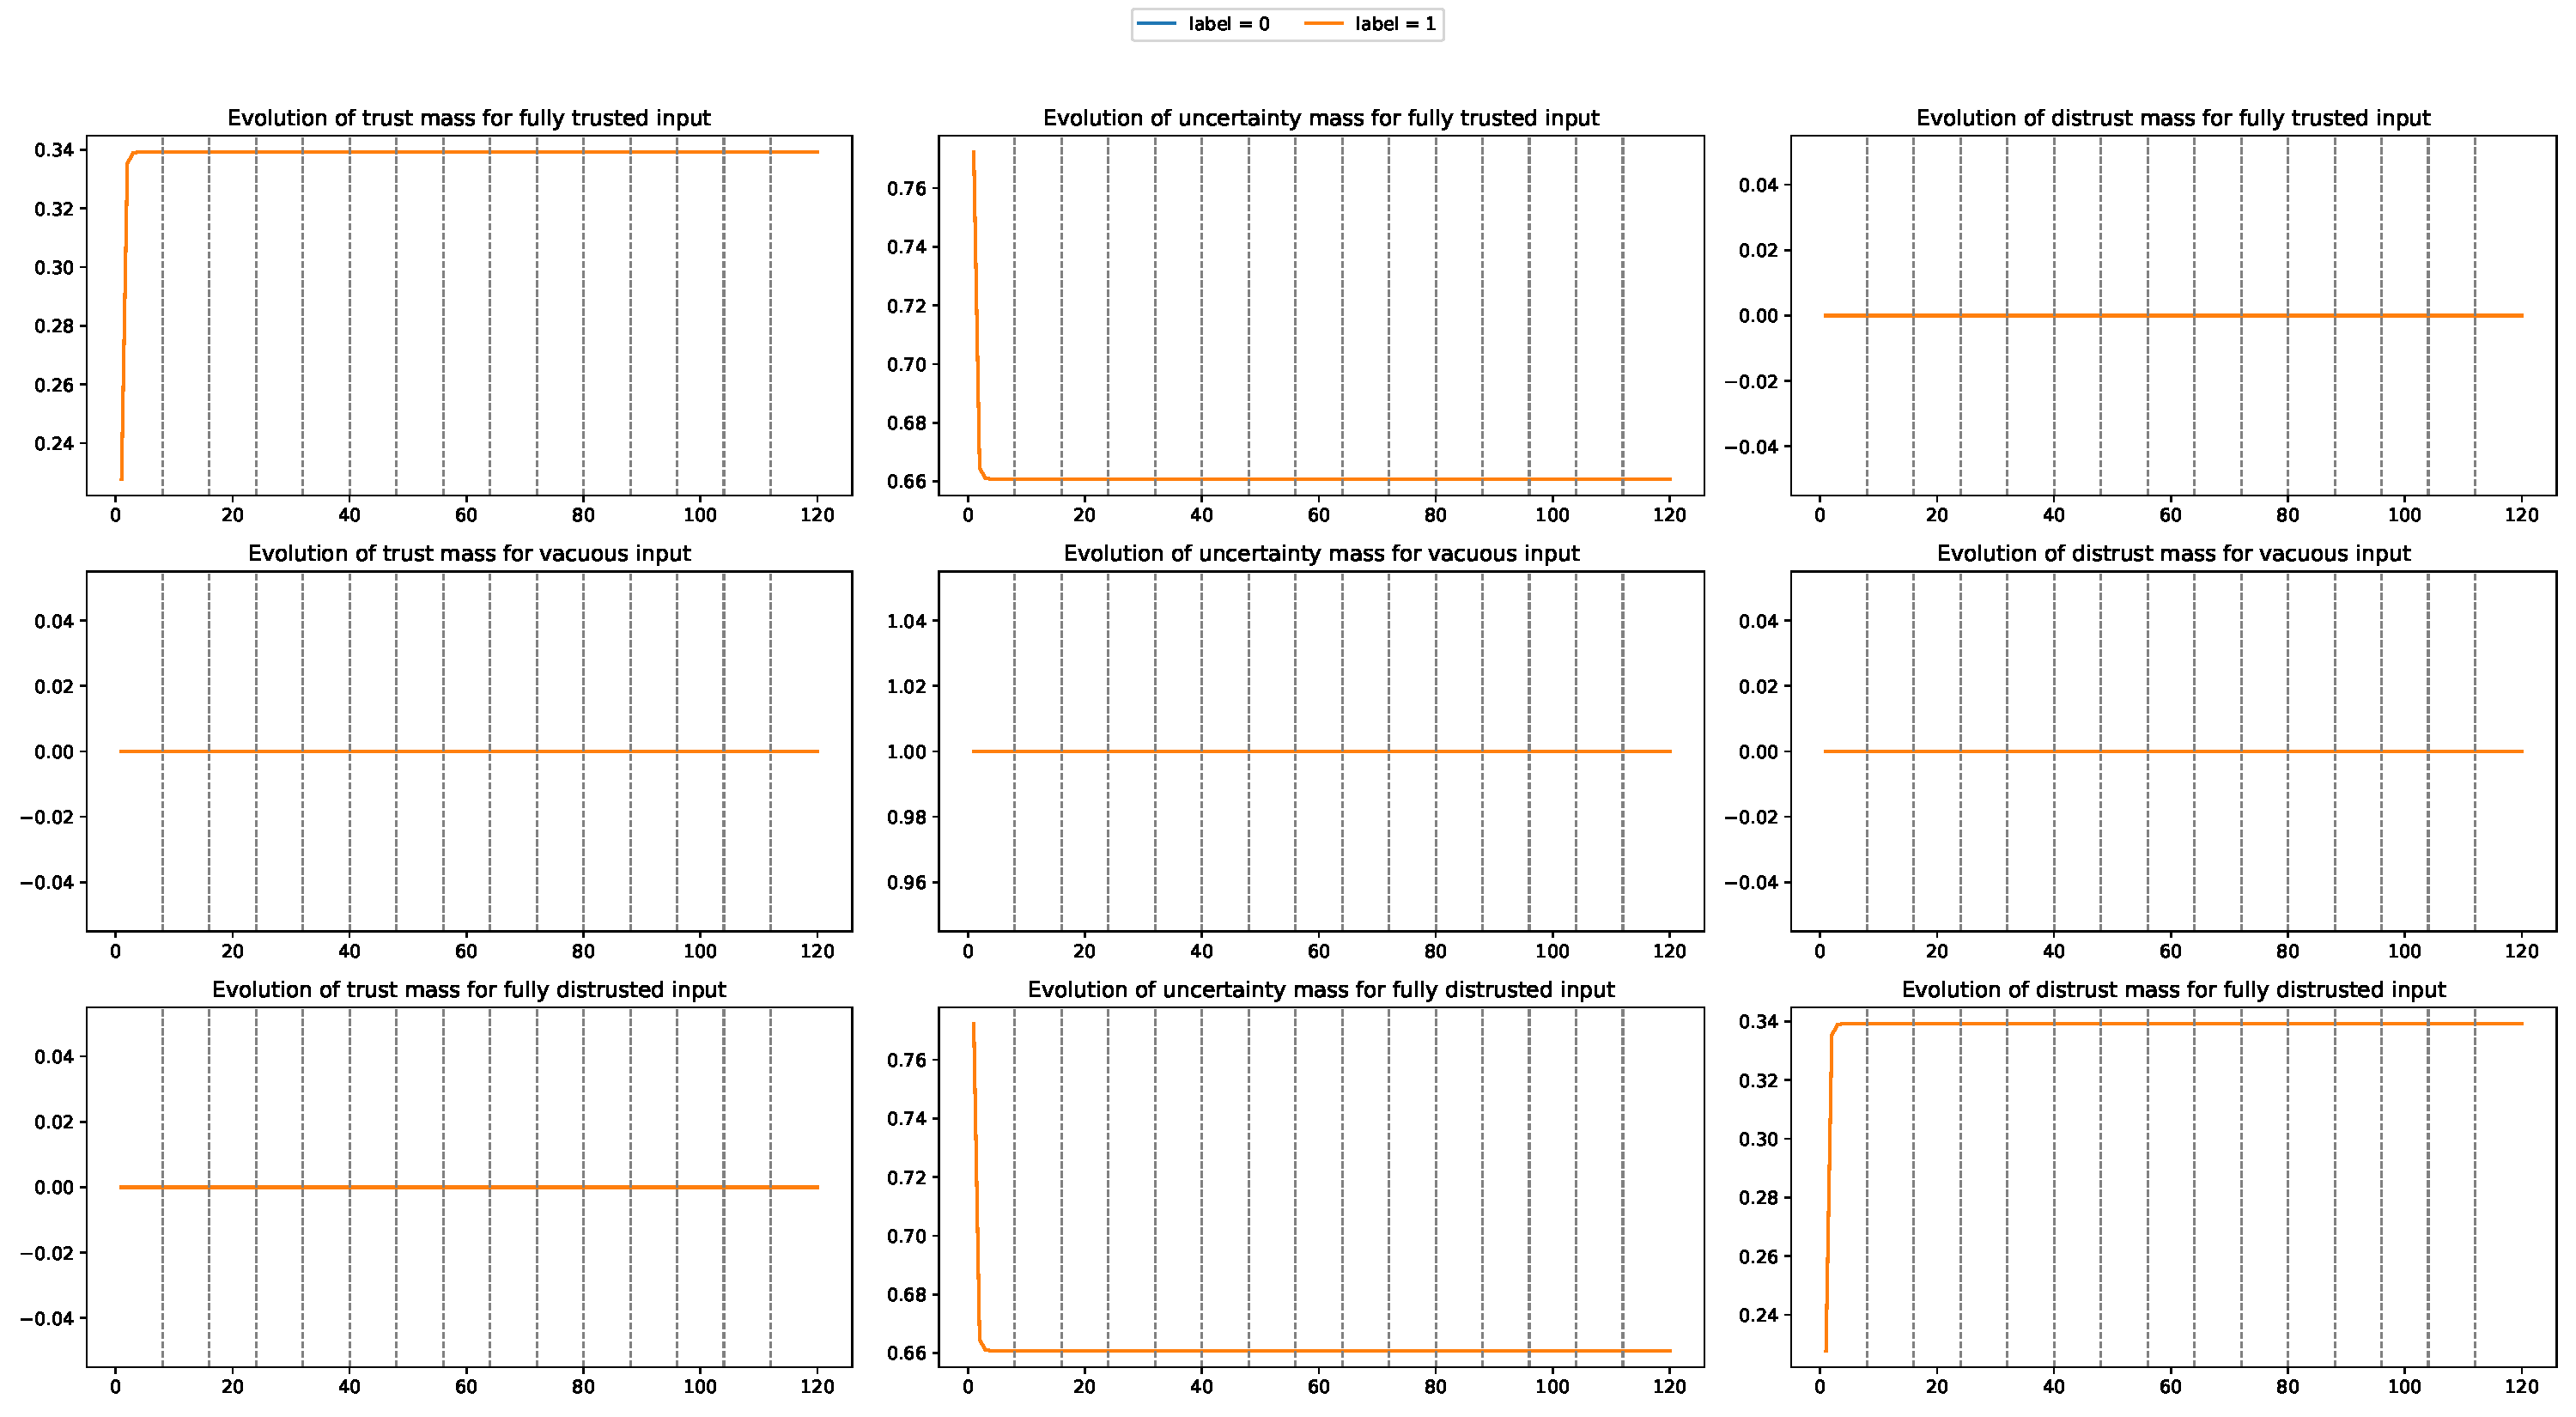
\includegraphics[width=0.8\textwidth]{latex/PTAS_Eval_cancer_16_vacuous_trust_eps_1_PathSize_None__plot_ptas.pdf}
\caption{cancer\_16\_vacuous\_trust, $\varepsilon$=1}
\end{figure}

\subsubsection{vacuous -- vacuous}

\begin{figure}[htbp]
\centering
  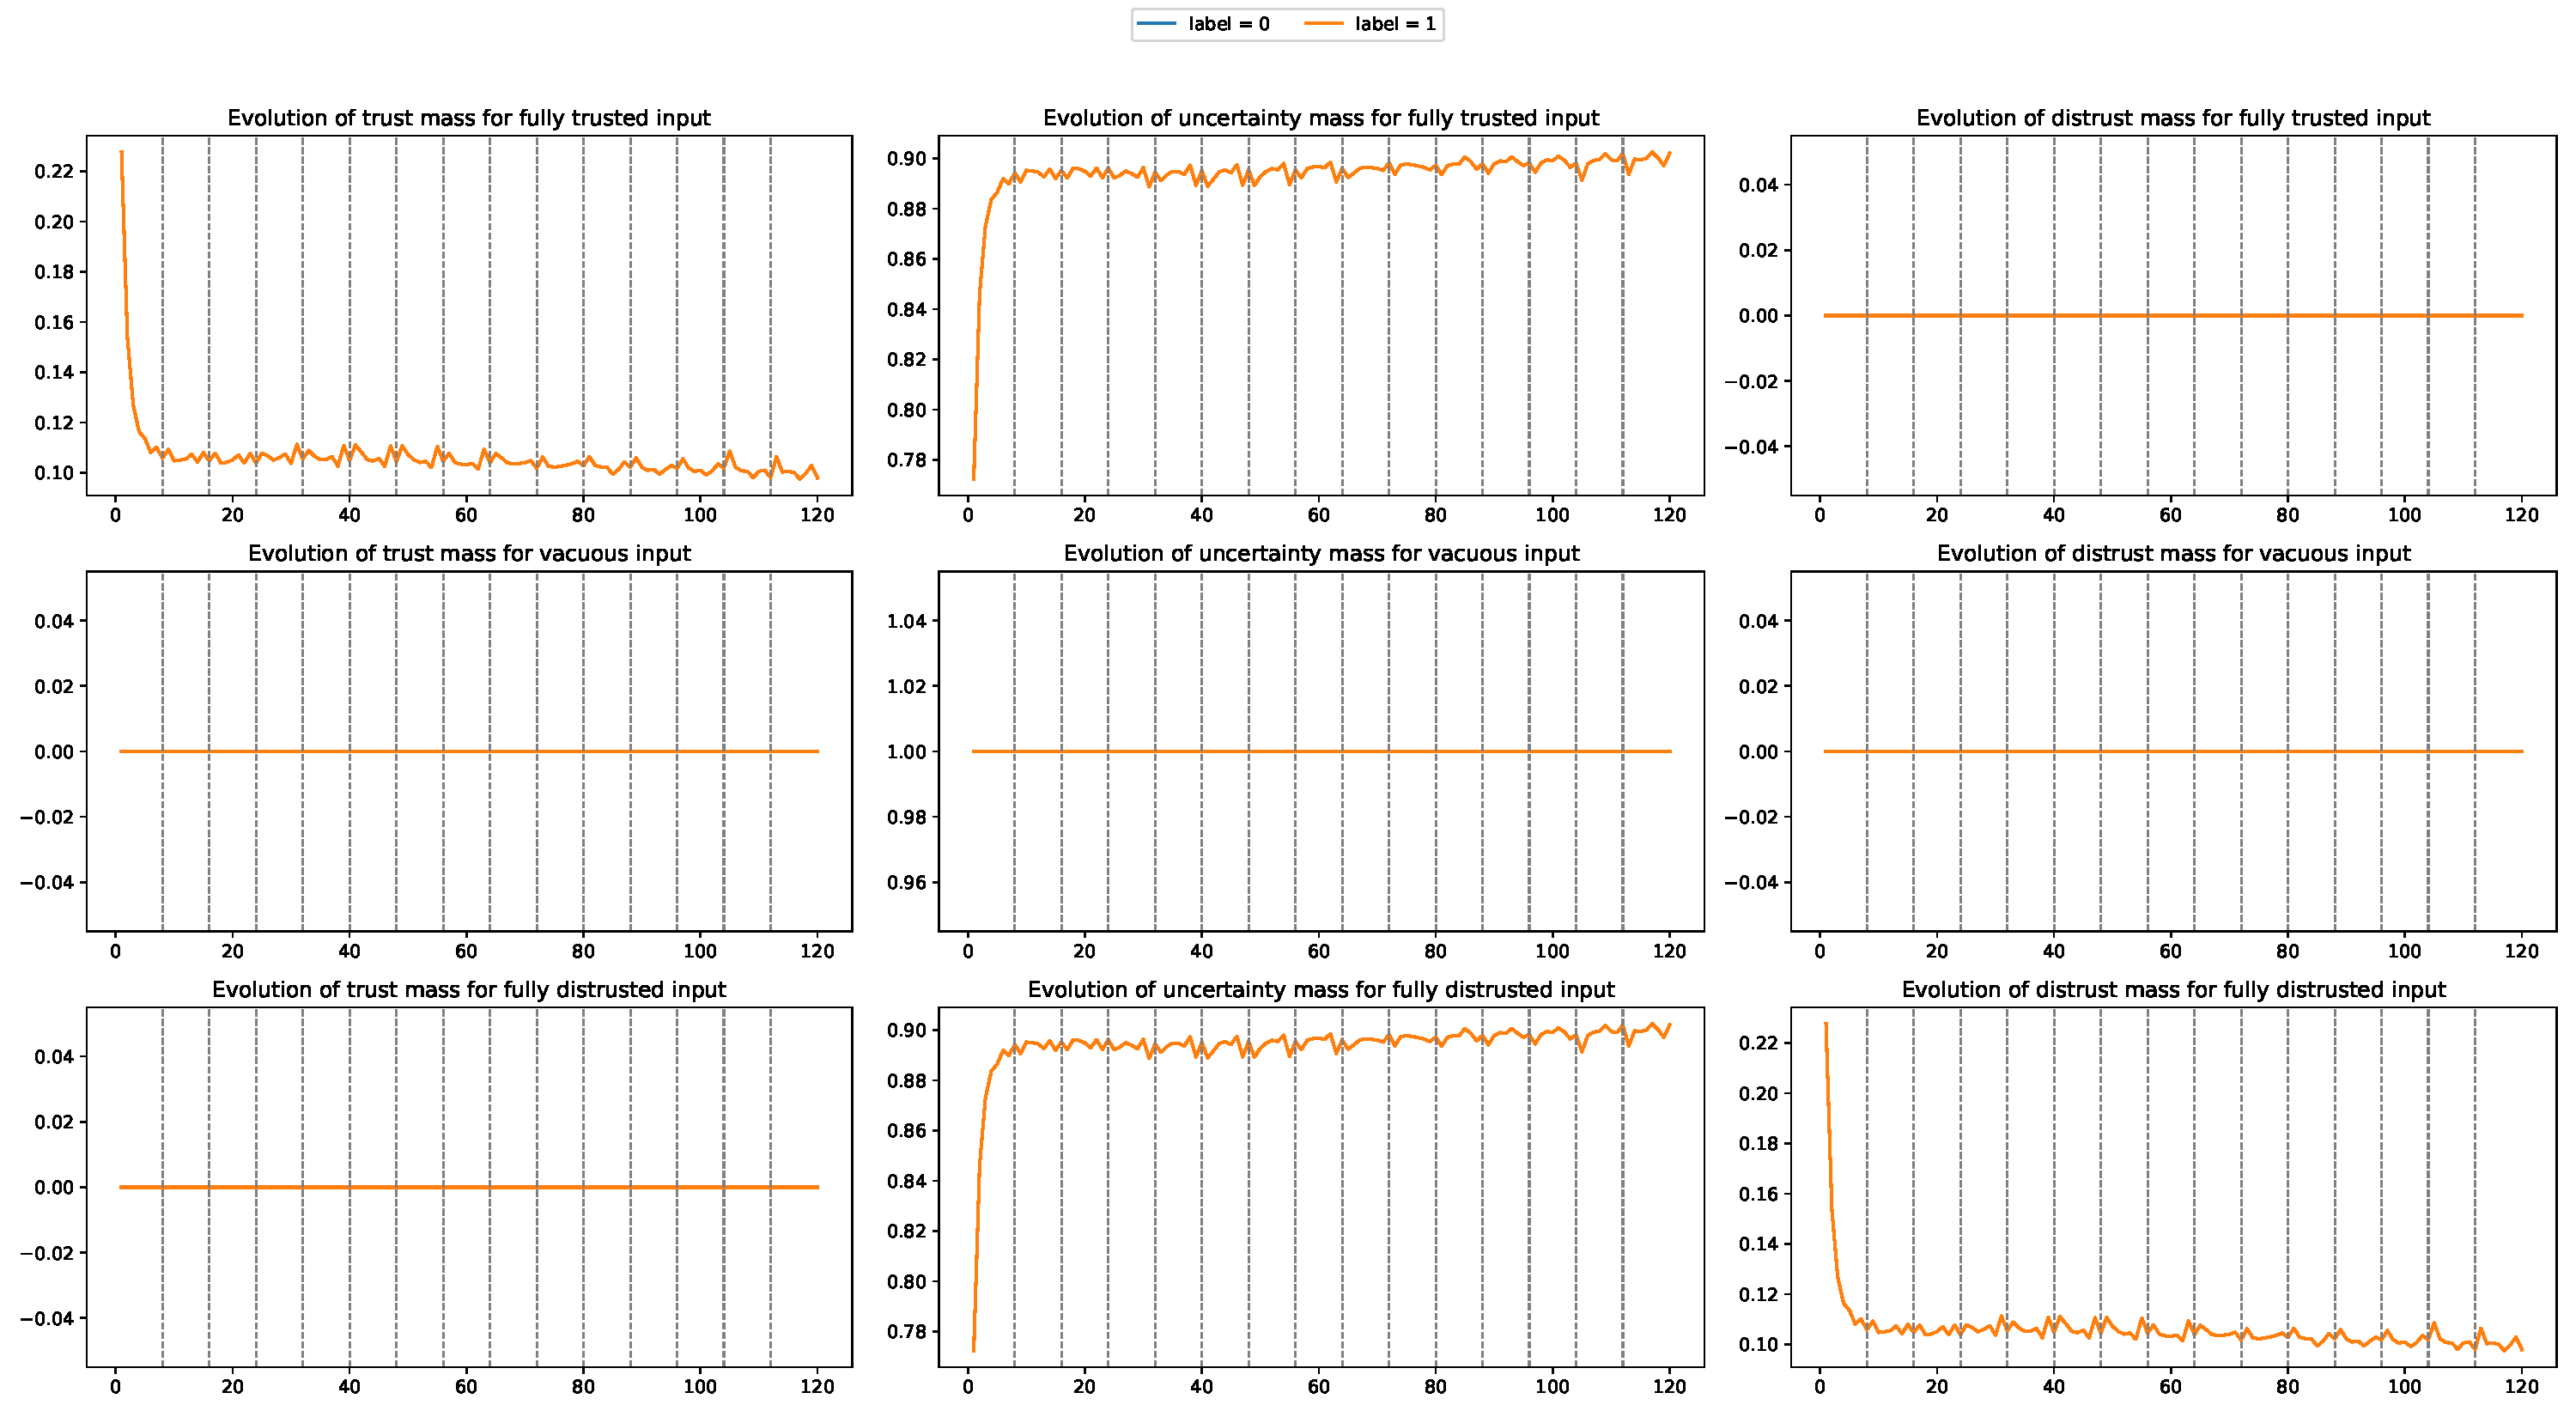
\includegraphics[width=0.8\textwidth]{latex/PTAS_Eval_cancer_16_vacuous_vacuous_eps_0.001_PathSize_None__plot_ptas.pdf}
\caption{cancer\_16\_vacuous\_vacuous, $\varepsilon$=0.001}
\end{figure}

\begin{figure}[htbp]
\centering
  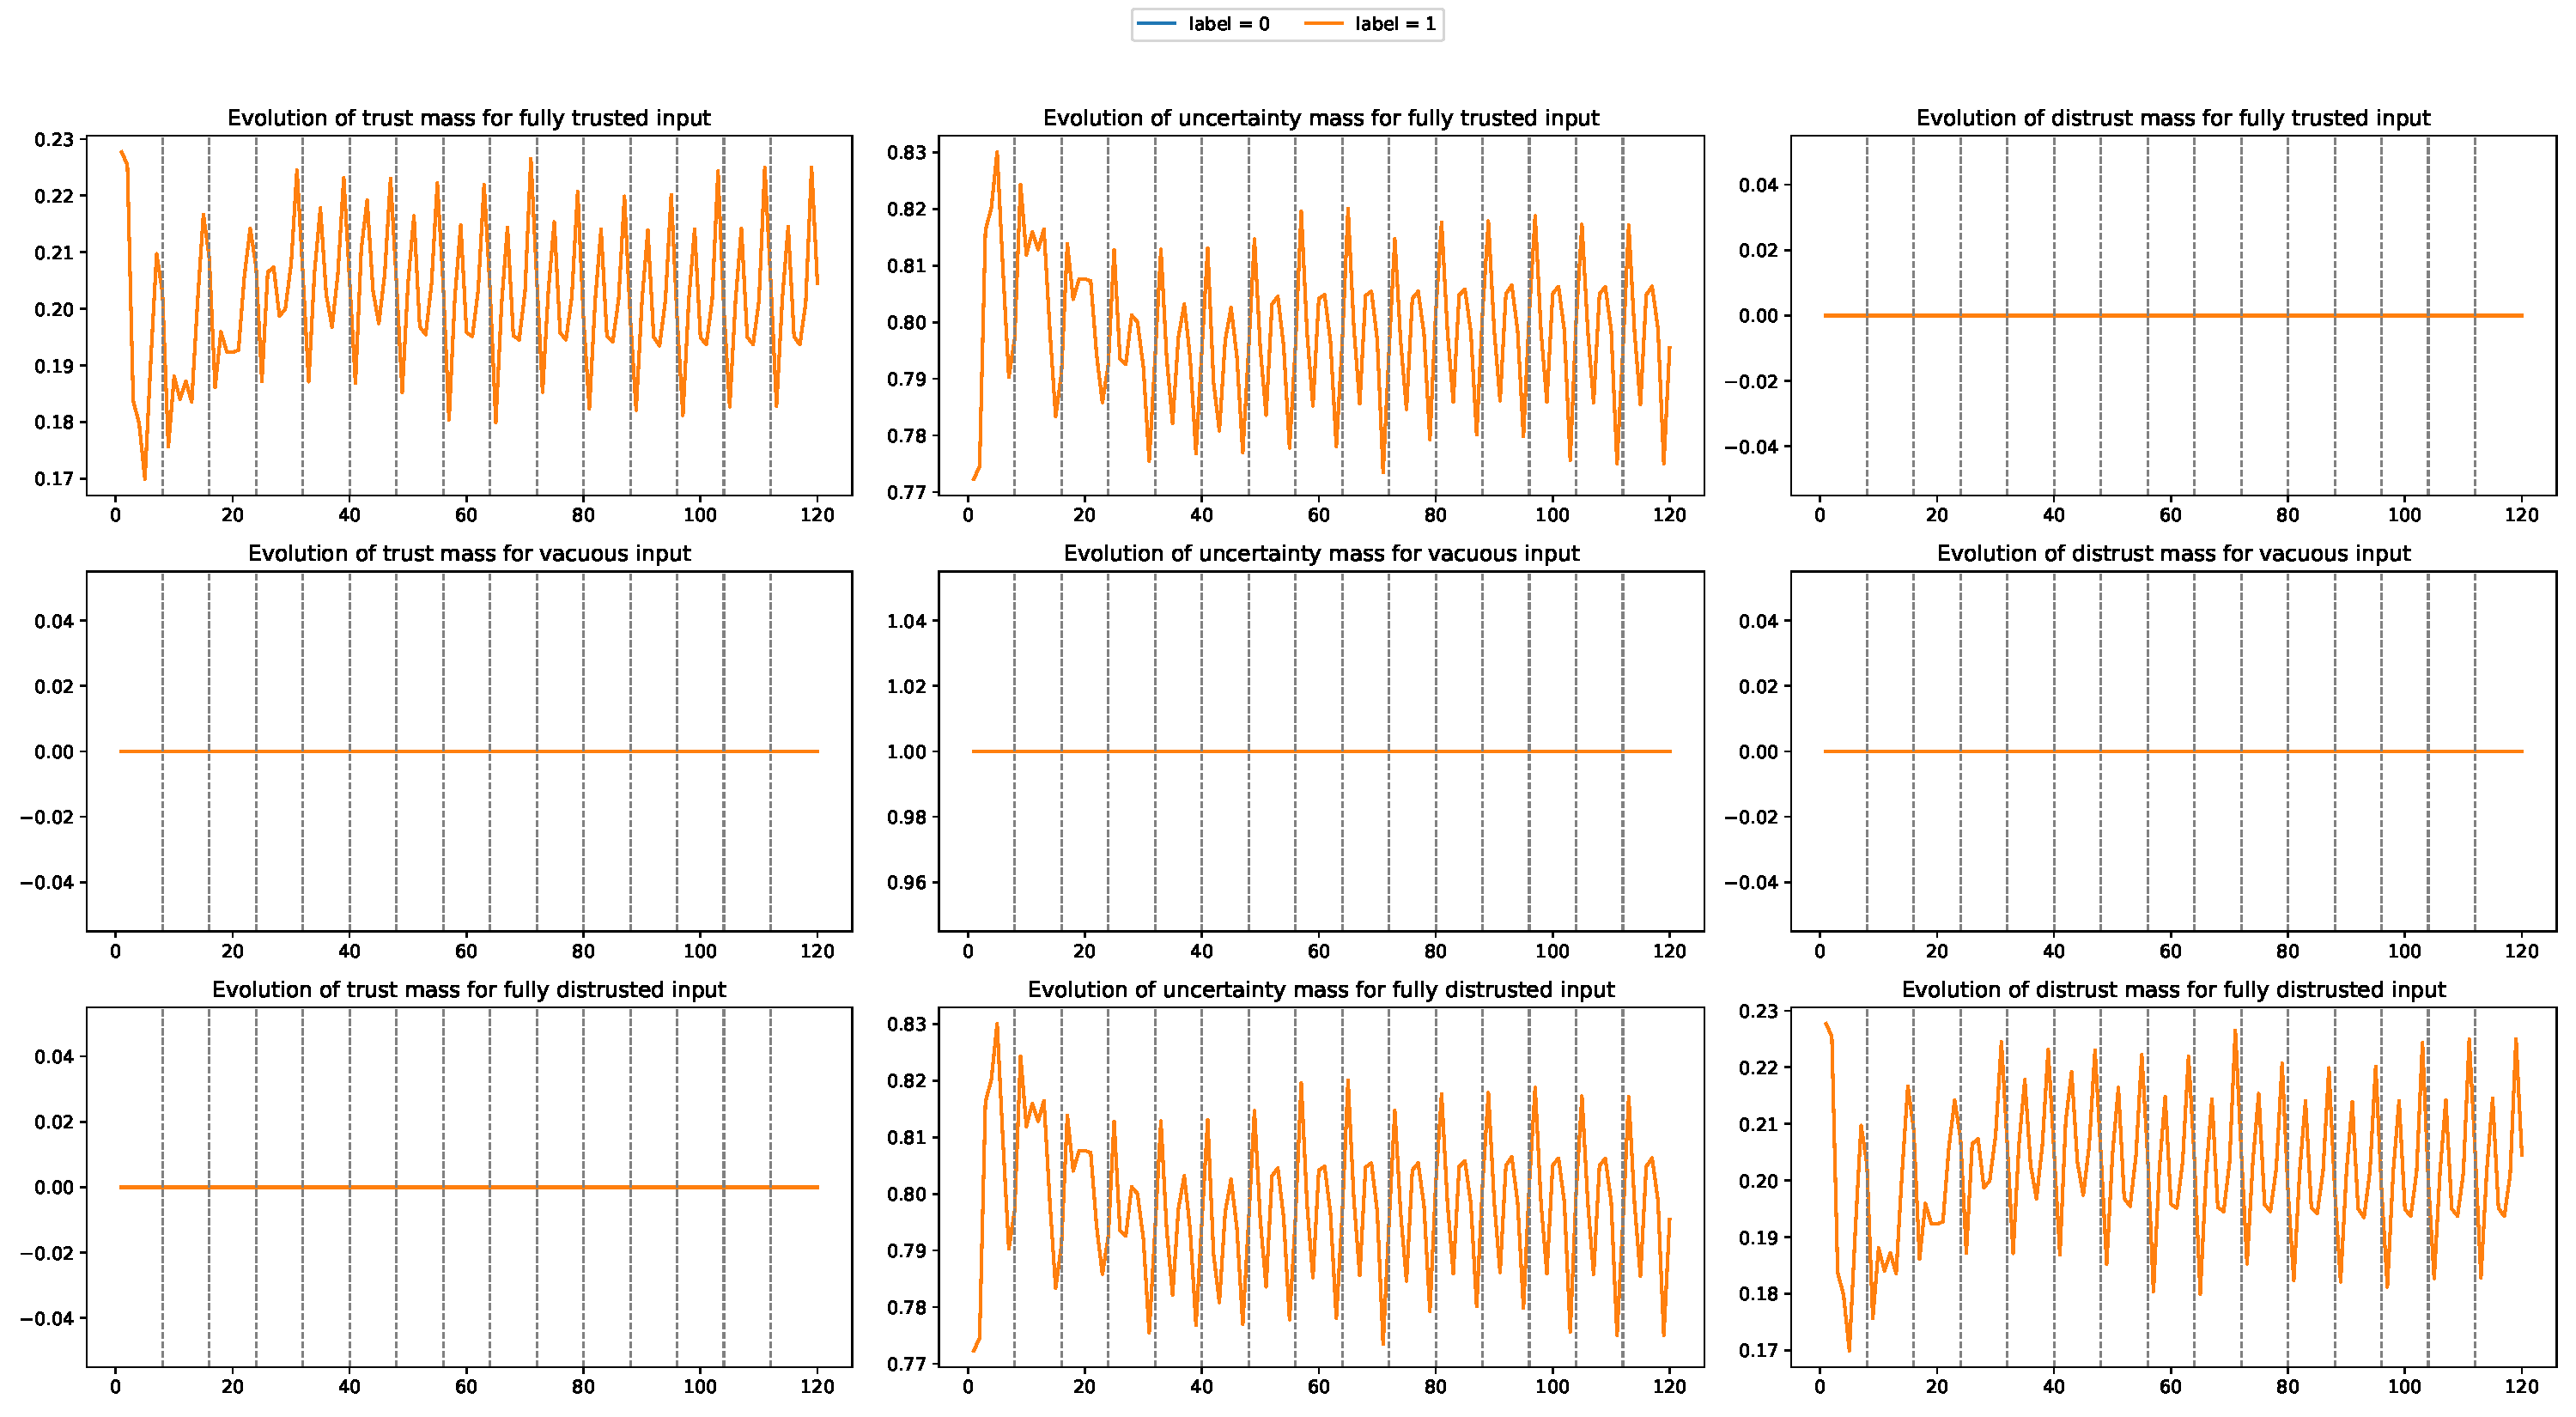
\includegraphics[width=0.8\textwidth]{latex/PTAS_Eval_cancer_16_vacuous_vacuous_eps_0.01_PathSize_None__plot_ptas.pdf}
\caption{cancer\_16\_vacuous\_vacuous, $\varepsilon$=0.01}
\end{figure}

\begin{figure}[htbp]
\centering
  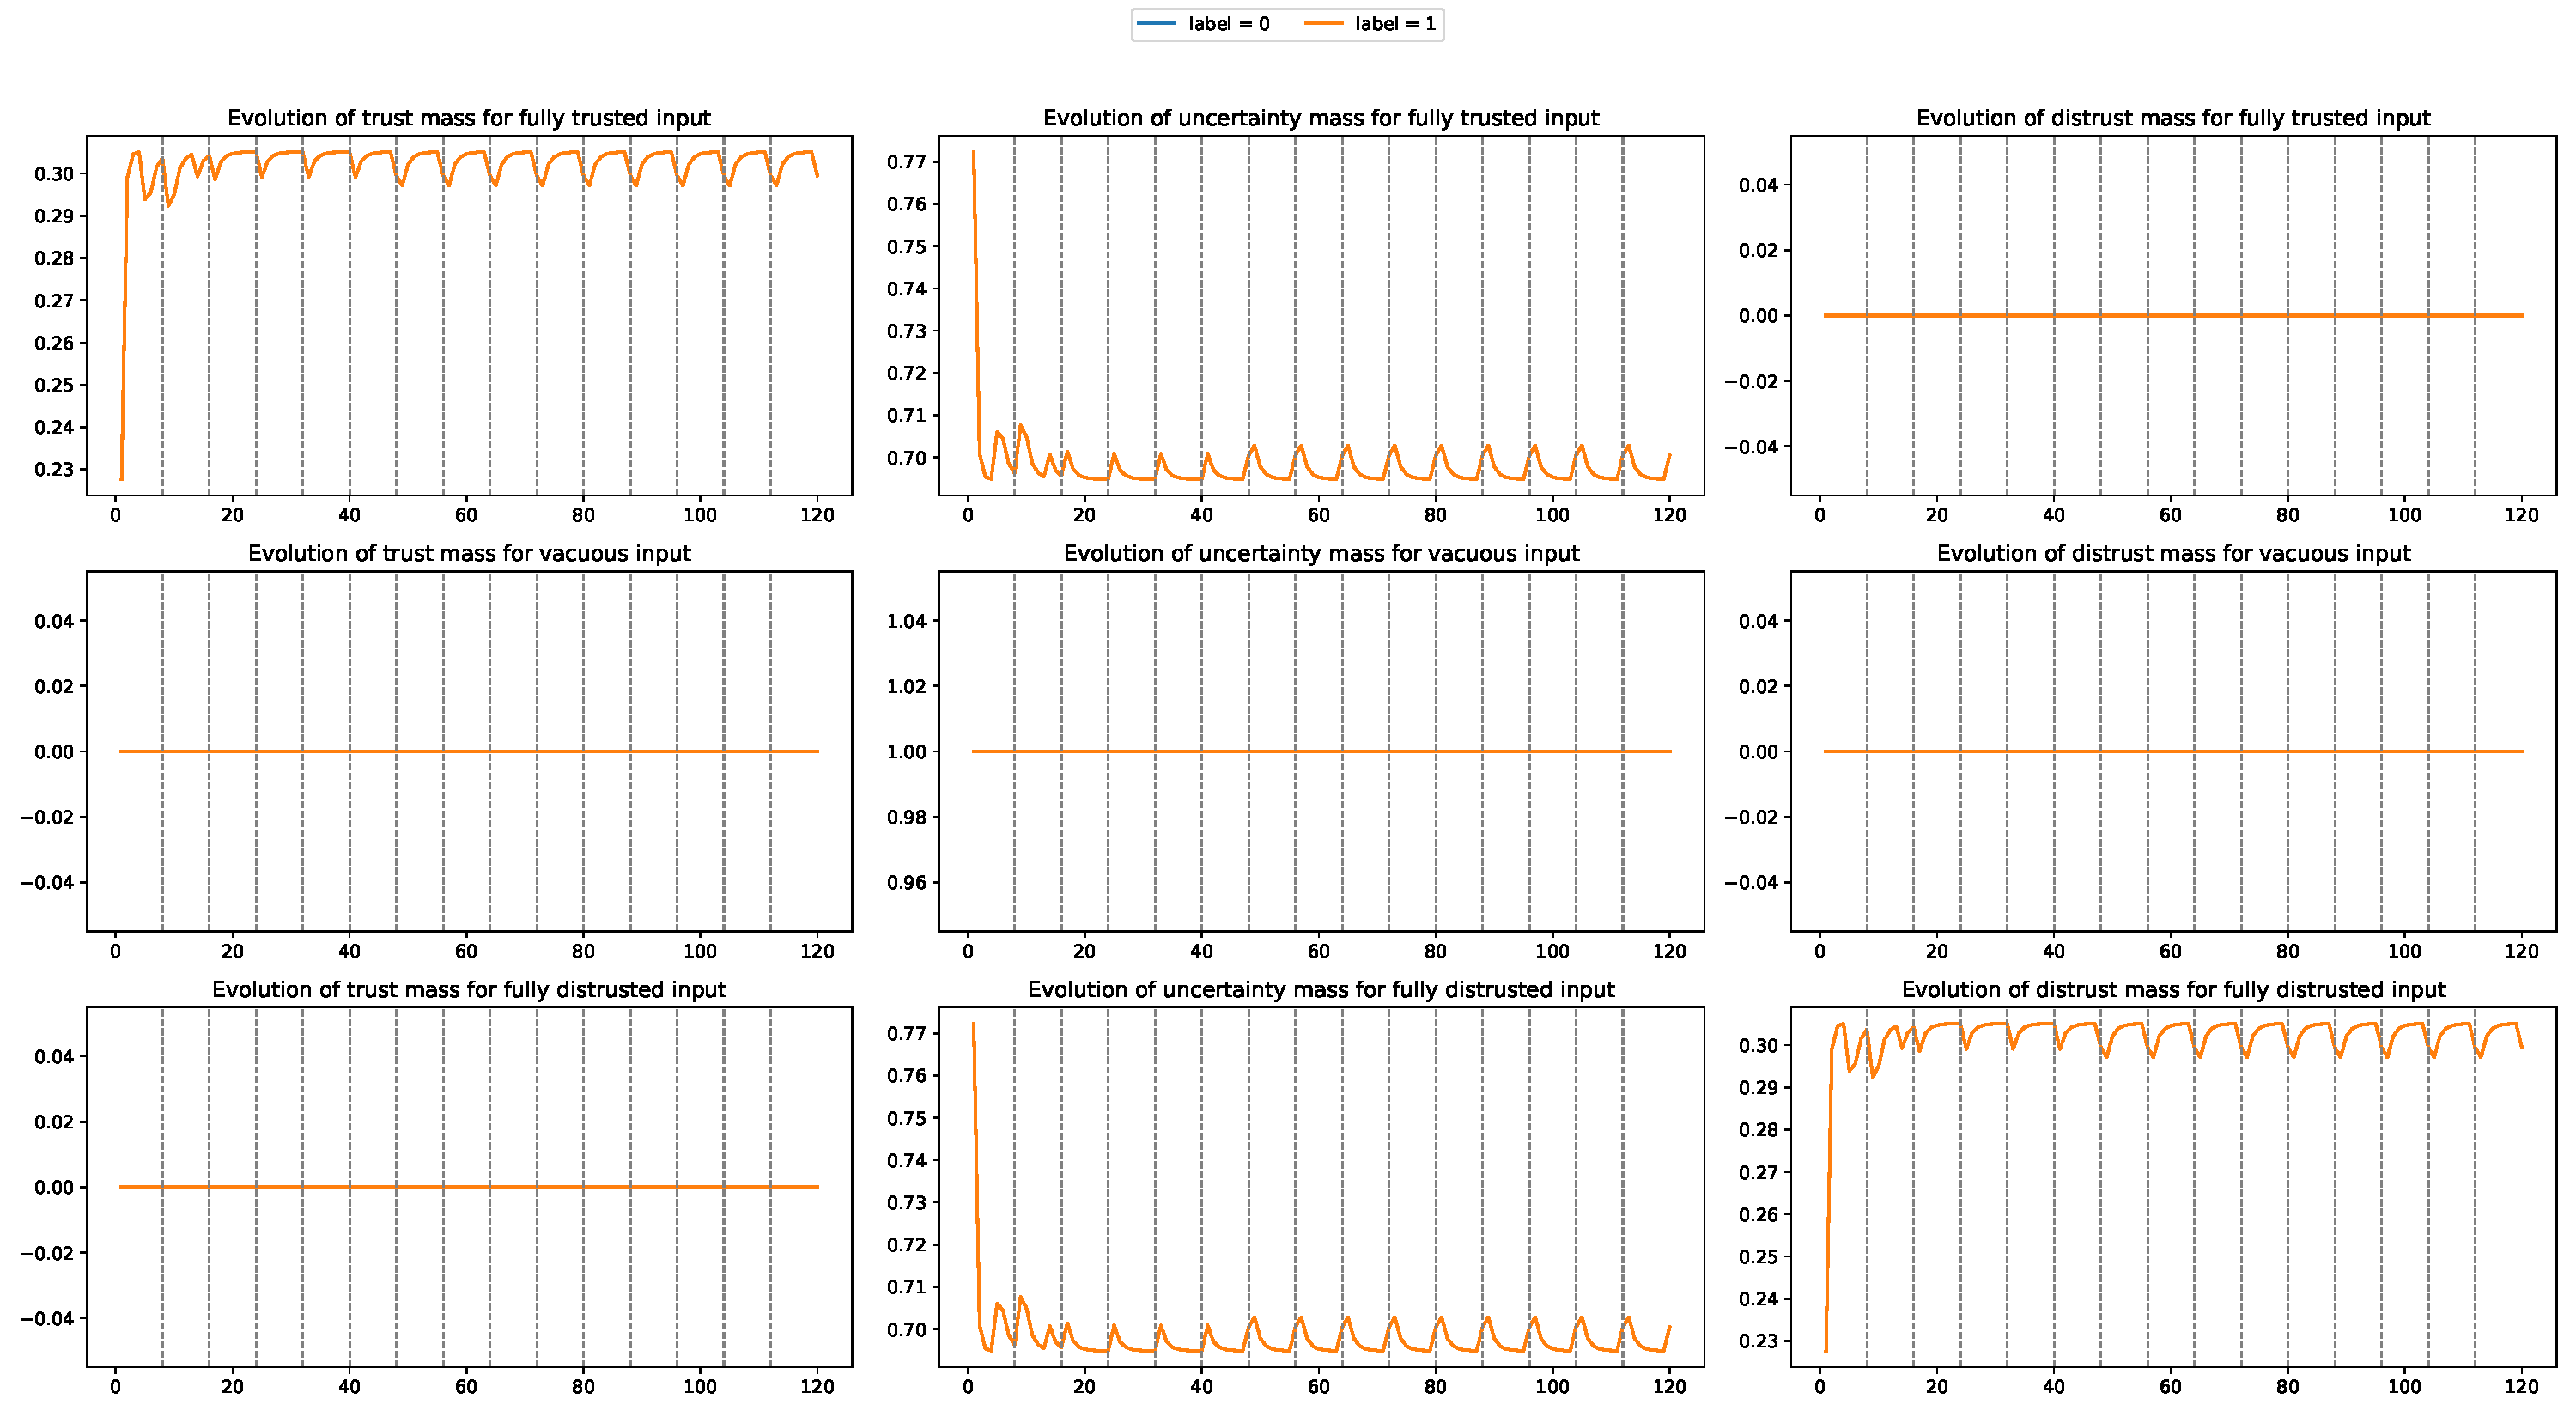
\includegraphics[width=0.8\textwidth]{latex/PTAS_Eval_cancer_16_vacuous_vacuous_eps_0.1_PathSize_None__plot_ptas.pdf}
\caption{cancer\_16\_vacuous\_vacuous, $\varepsilon$=0.1}
\end{figure}

\begin{figure}[htbp]
\centering
  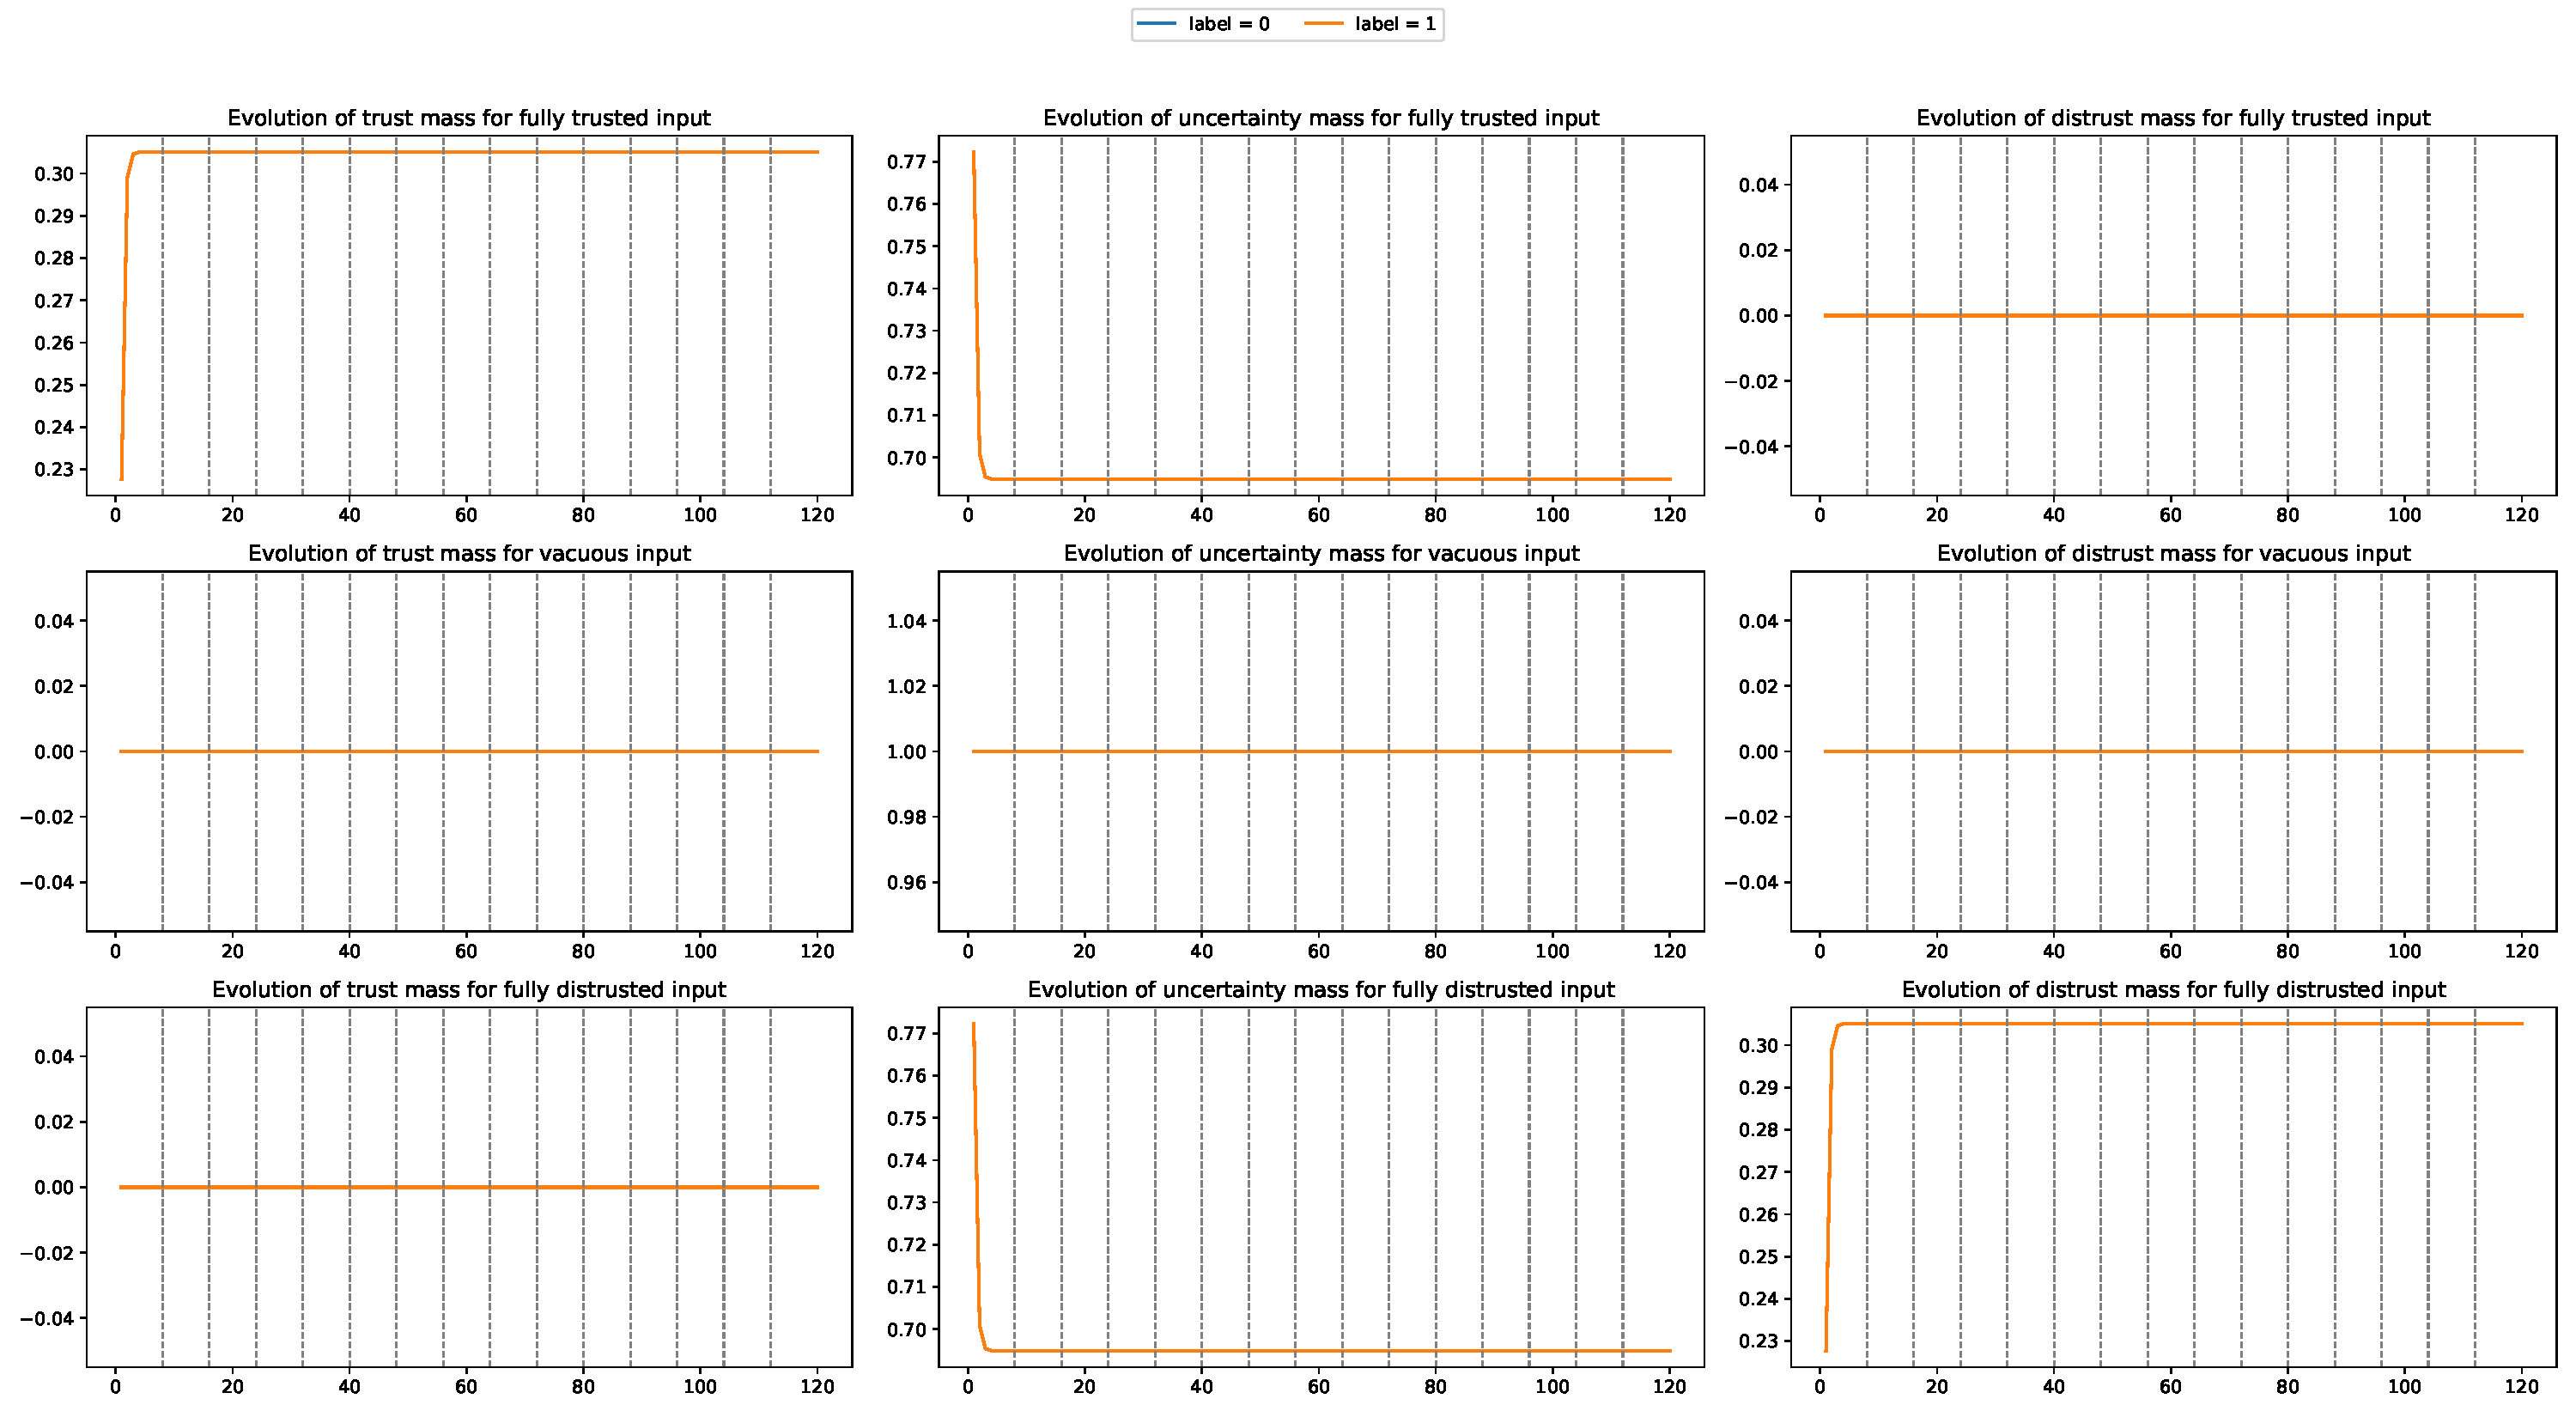
\includegraphics[width=0.8\textwidth]{latex/PTAS_Eval_cancer_16_vacuous_vacuous_eps_1_PathSize_None__plot_ptas.pdf}
\caption{cancer\_16\_vacuous\_vacuous, $\varepsilon$=1}
\end{figure}

\subsection{MNIST Dataset}

\subsubsection{trust -- trust}

\begin{figure}[htbp]
\centering
  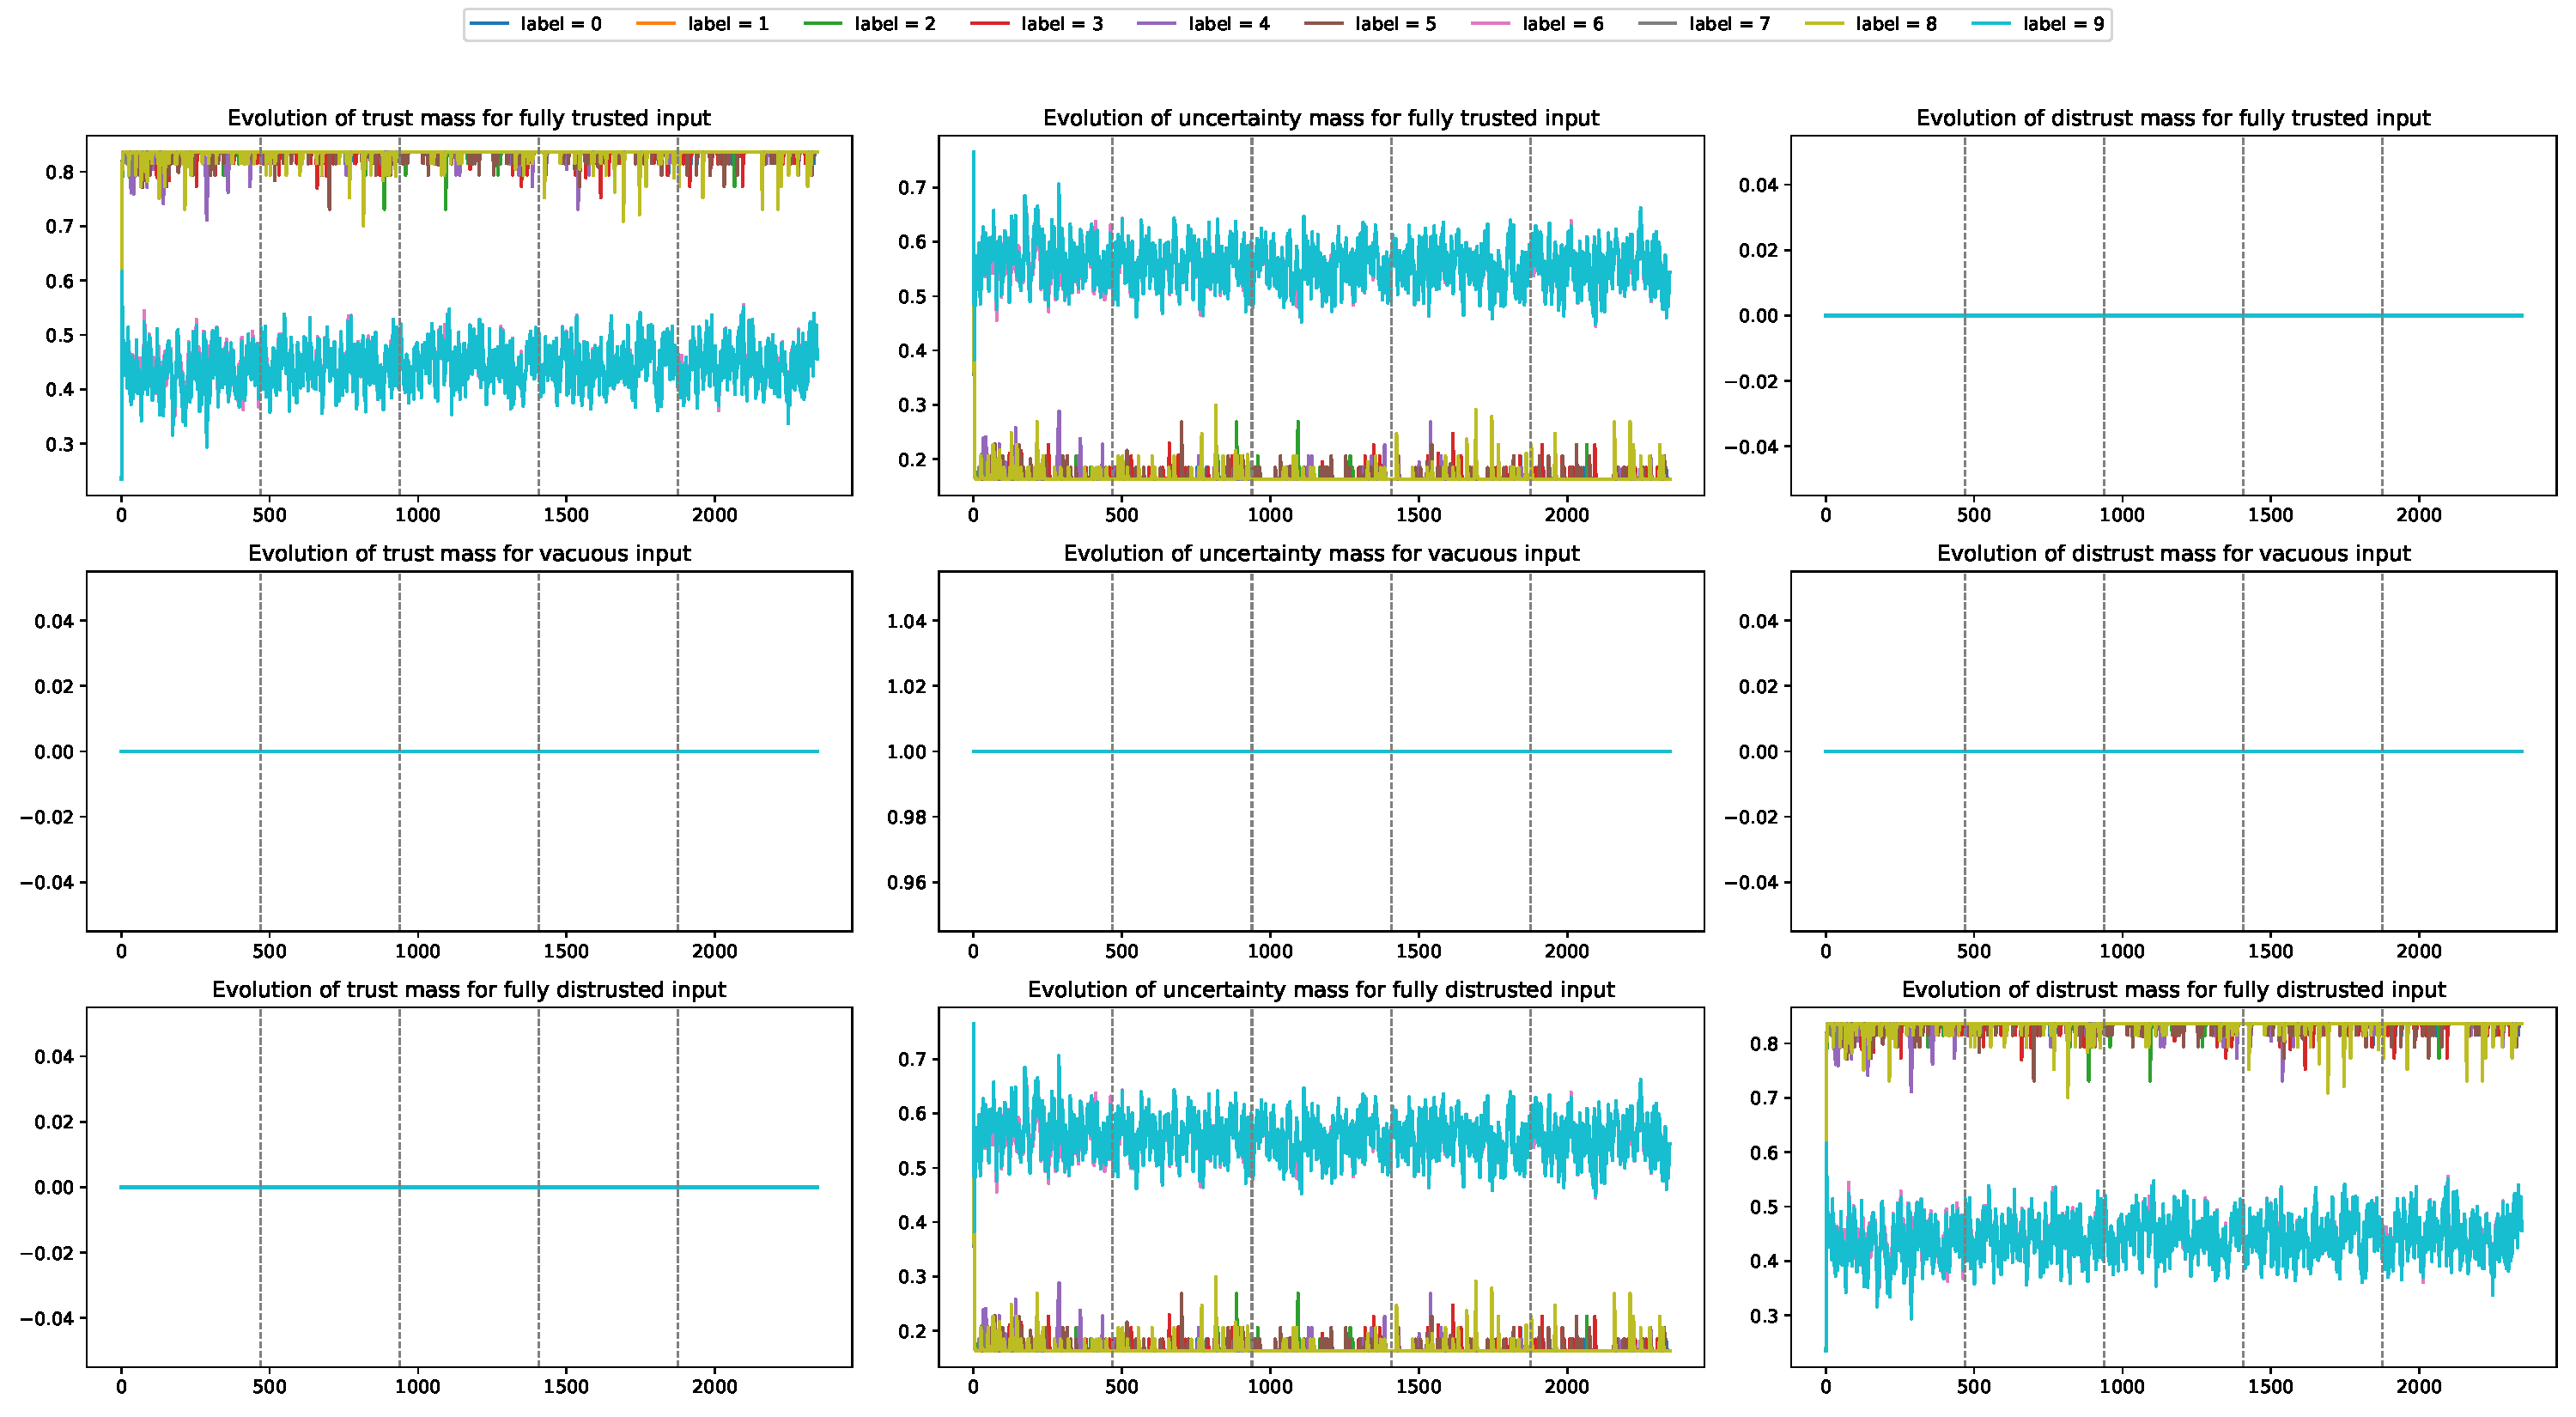
\includegraphics[width=0.8\textwidth]{latex/PTAS_Eval_mnist_128_trust_trust_eps_0.05_PathSize_1__plot_ptas.pdf}
\caption{mnist\_128\_trust\_trust, $\varepsilon$=0.05, ps=1}
\end{figure}

\begin{figure}[htbp]
\centering
  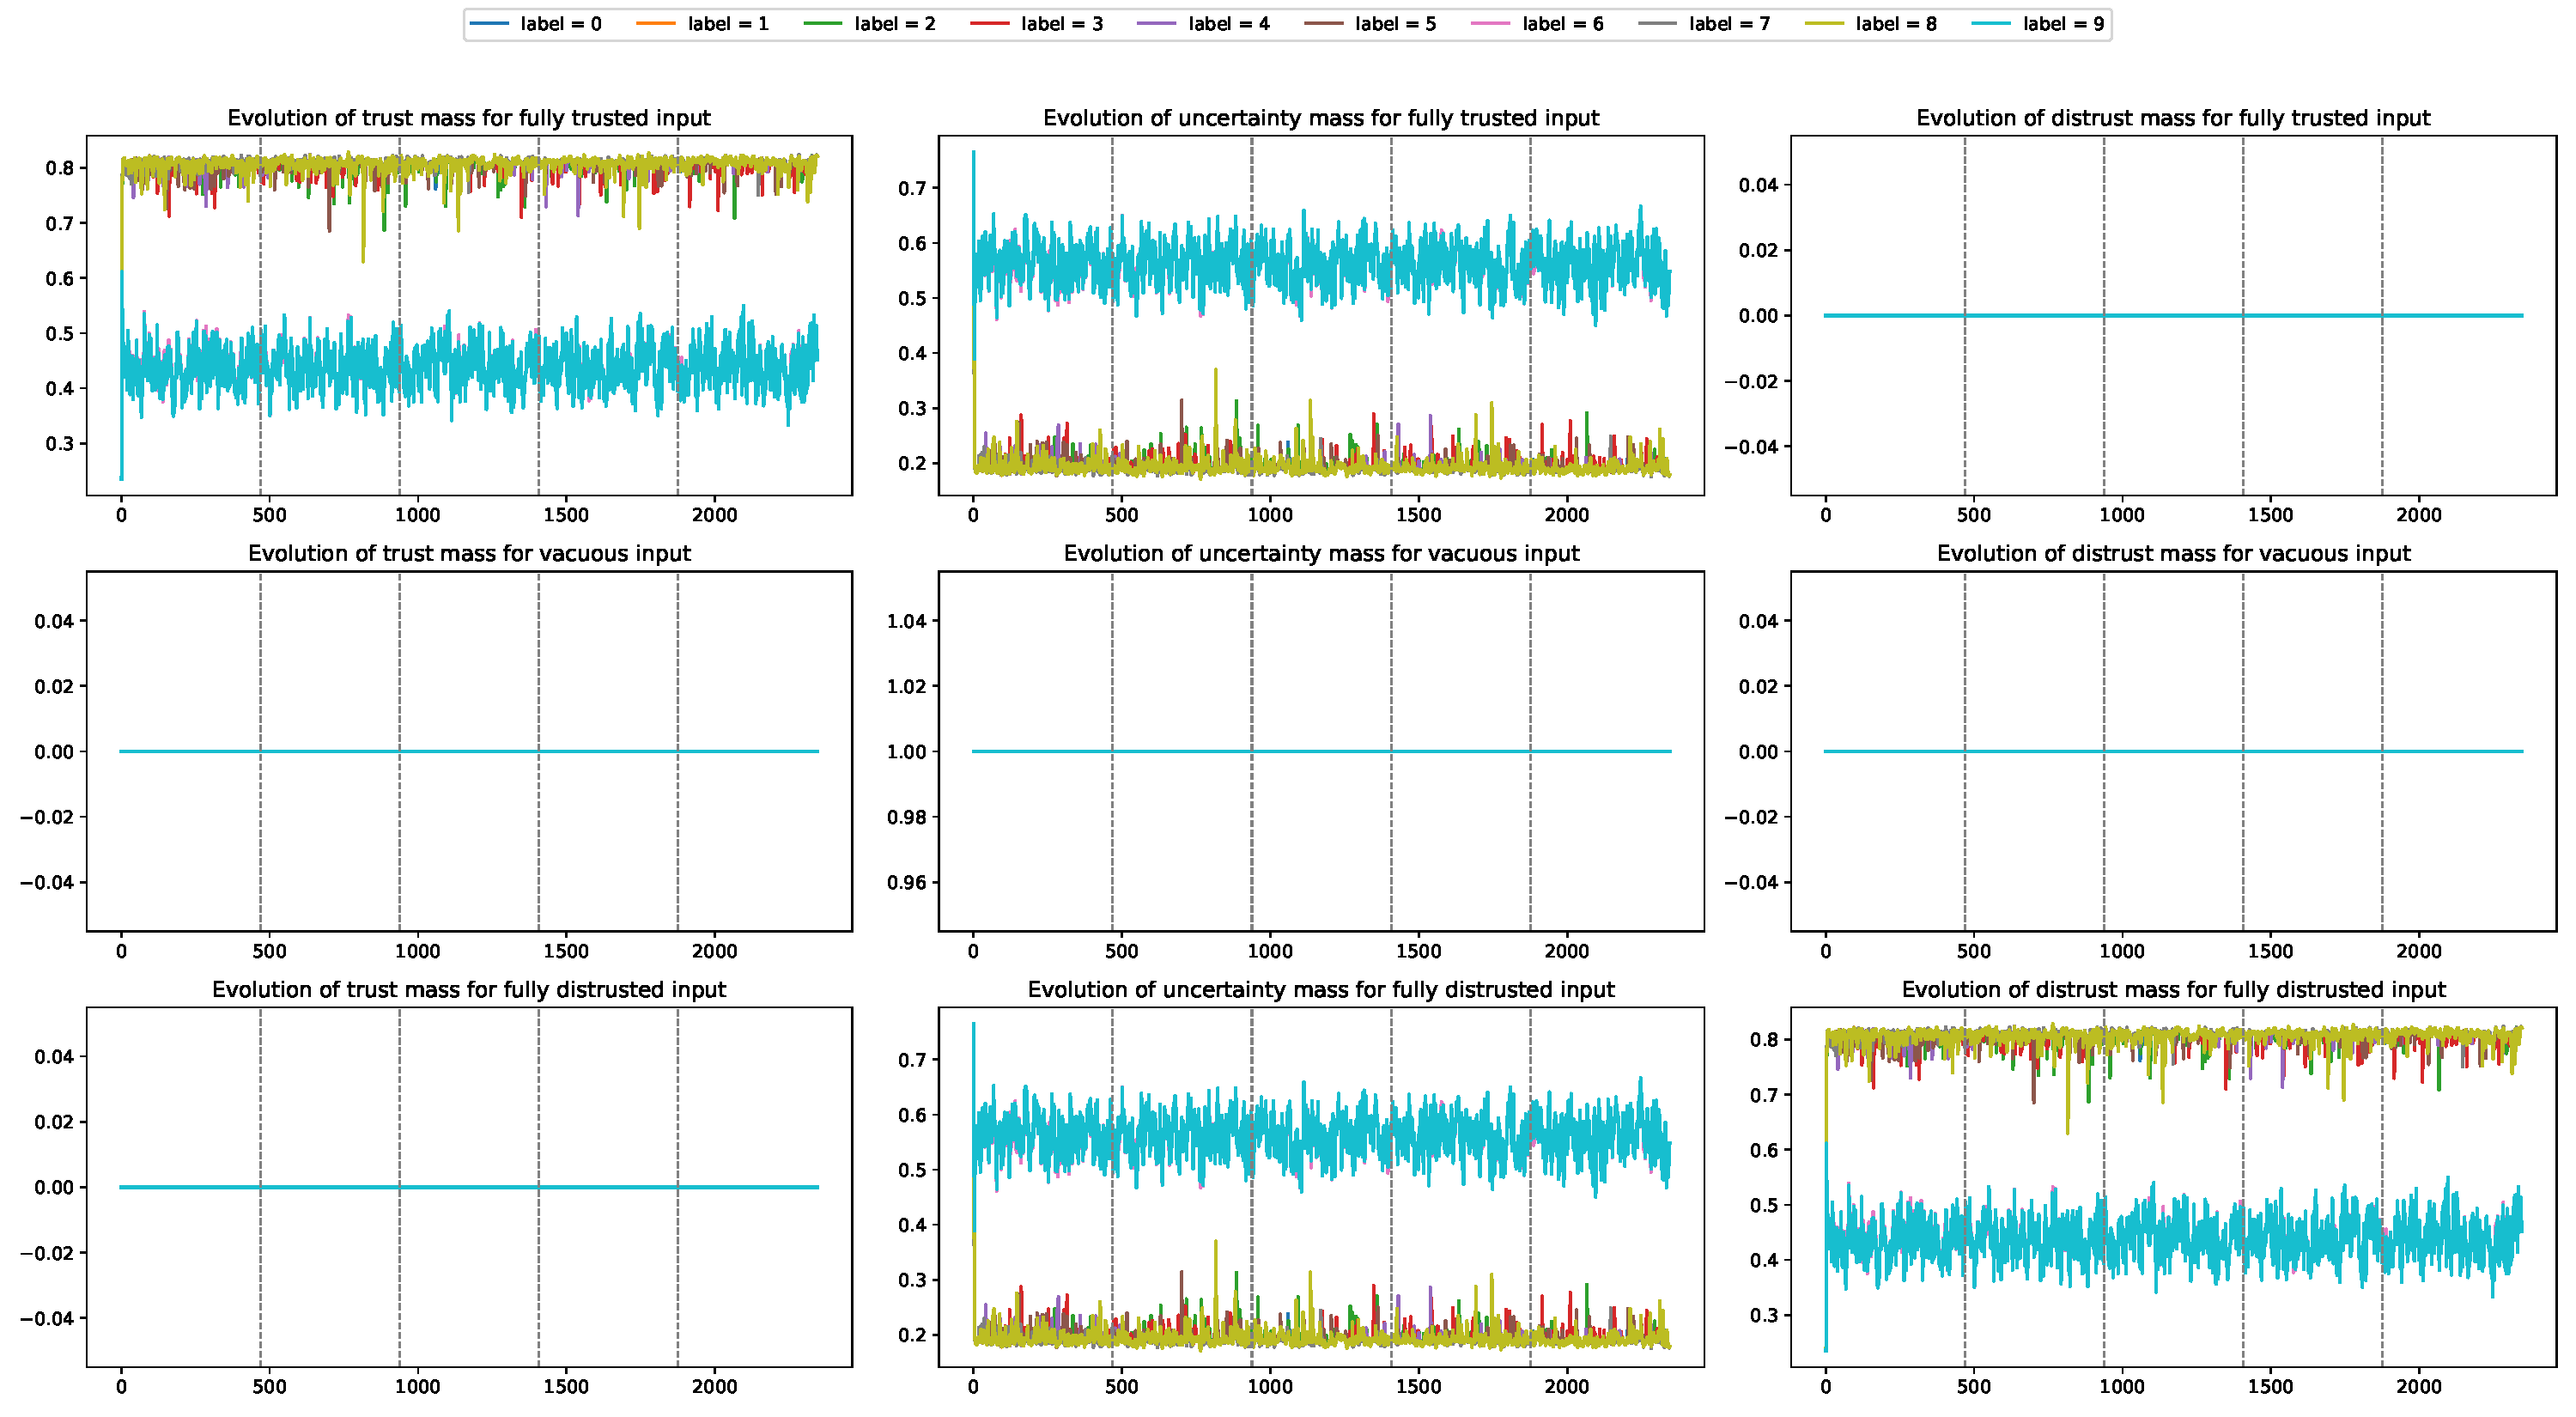
\includegraphics[width=0.8\textwidth]{latex/PTAS_Eval_mnist_128_trust_trust_eps_0.05_PathSize_10__plot_ptas.pdf}
\caption{mnist\_128\_trust\_trust, $\varepsilon$=0.05, ps=10}
\end{figure}

\begin{figure}[htbp]
\centering
  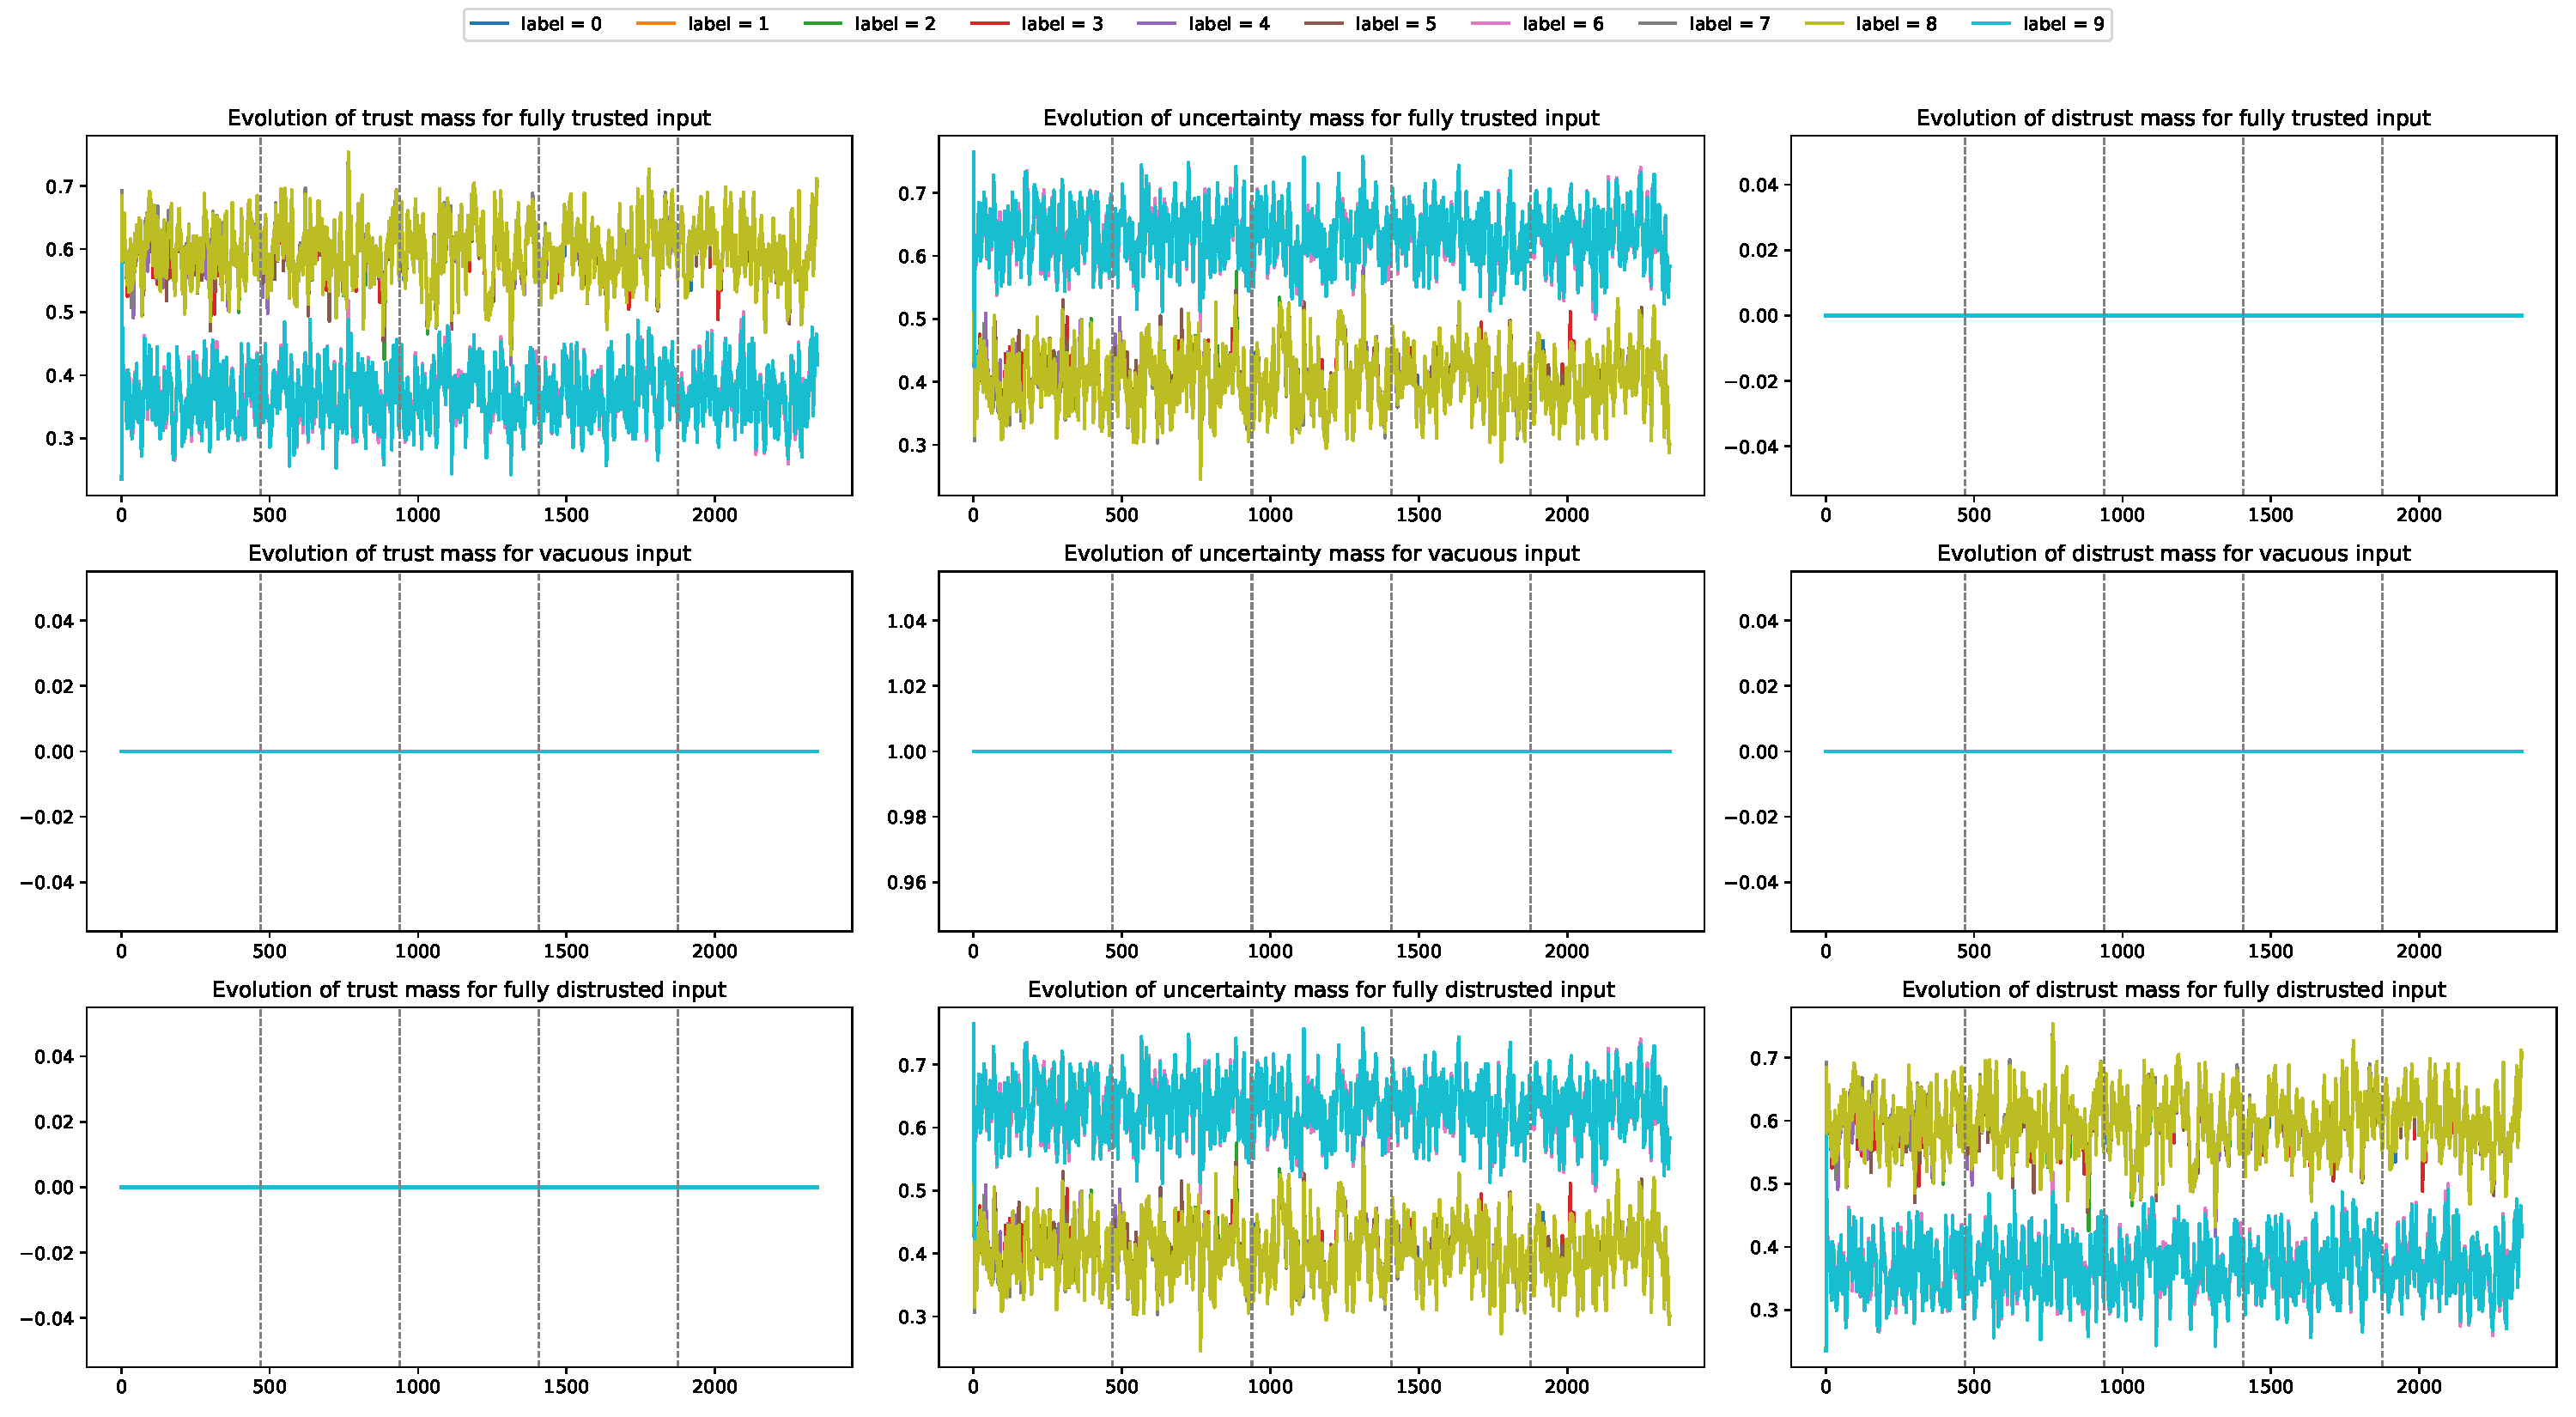
\includegraphics[width=0.8\textwidth]{latex/PTAS_Eval_mnist_128_trust_trust_eps_0.05_PathSize_27__plot_ptas.pdf}
\caption{mnist\_128\_trust\_trust, $\varepsilon$=0.05, ps=27}
\end{figure}

\begin{figure}[htbp]
\centering
  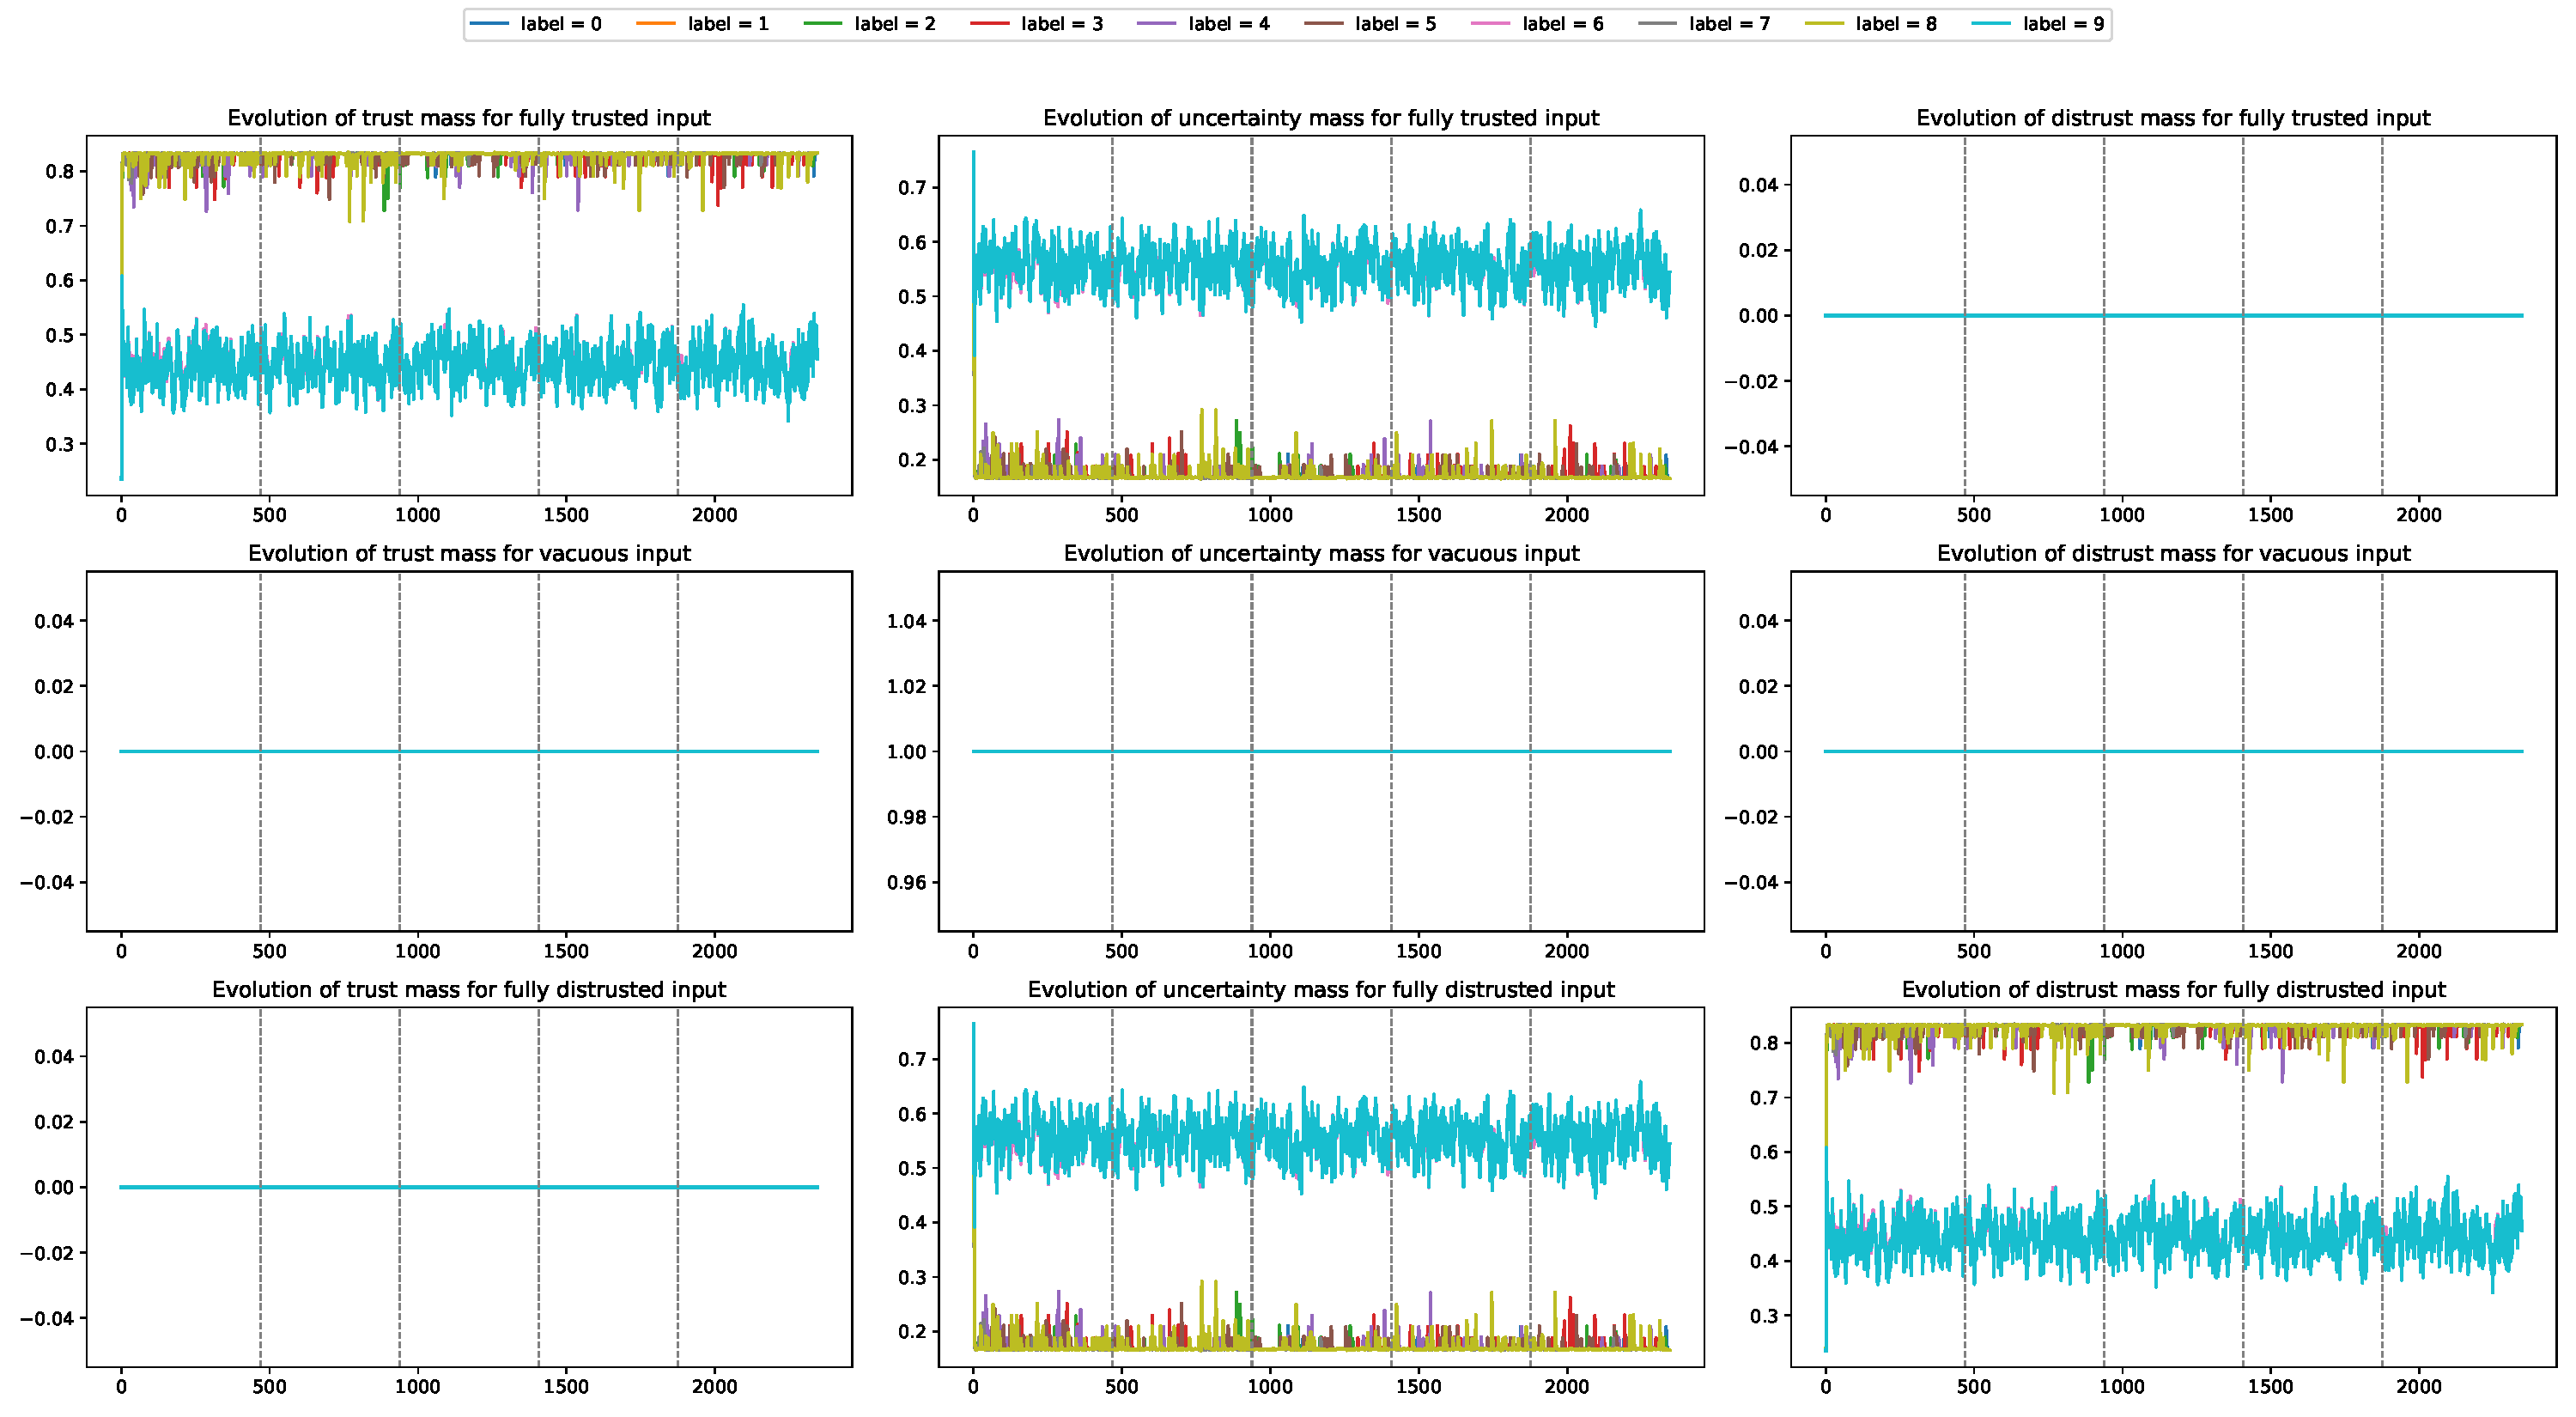
\includegraphics[width=0.8\textwidth]{latex/PTAS_Eval_mnist_128_trust_trust_eps_0.05_PathSize_4__plot_ptas.pdf}
\caption{mnist\_128\_trust\_trust, $\varepsilon$=0.05, ps=4}
\end{figure}

\begin{figure}[htbp]
\centering
  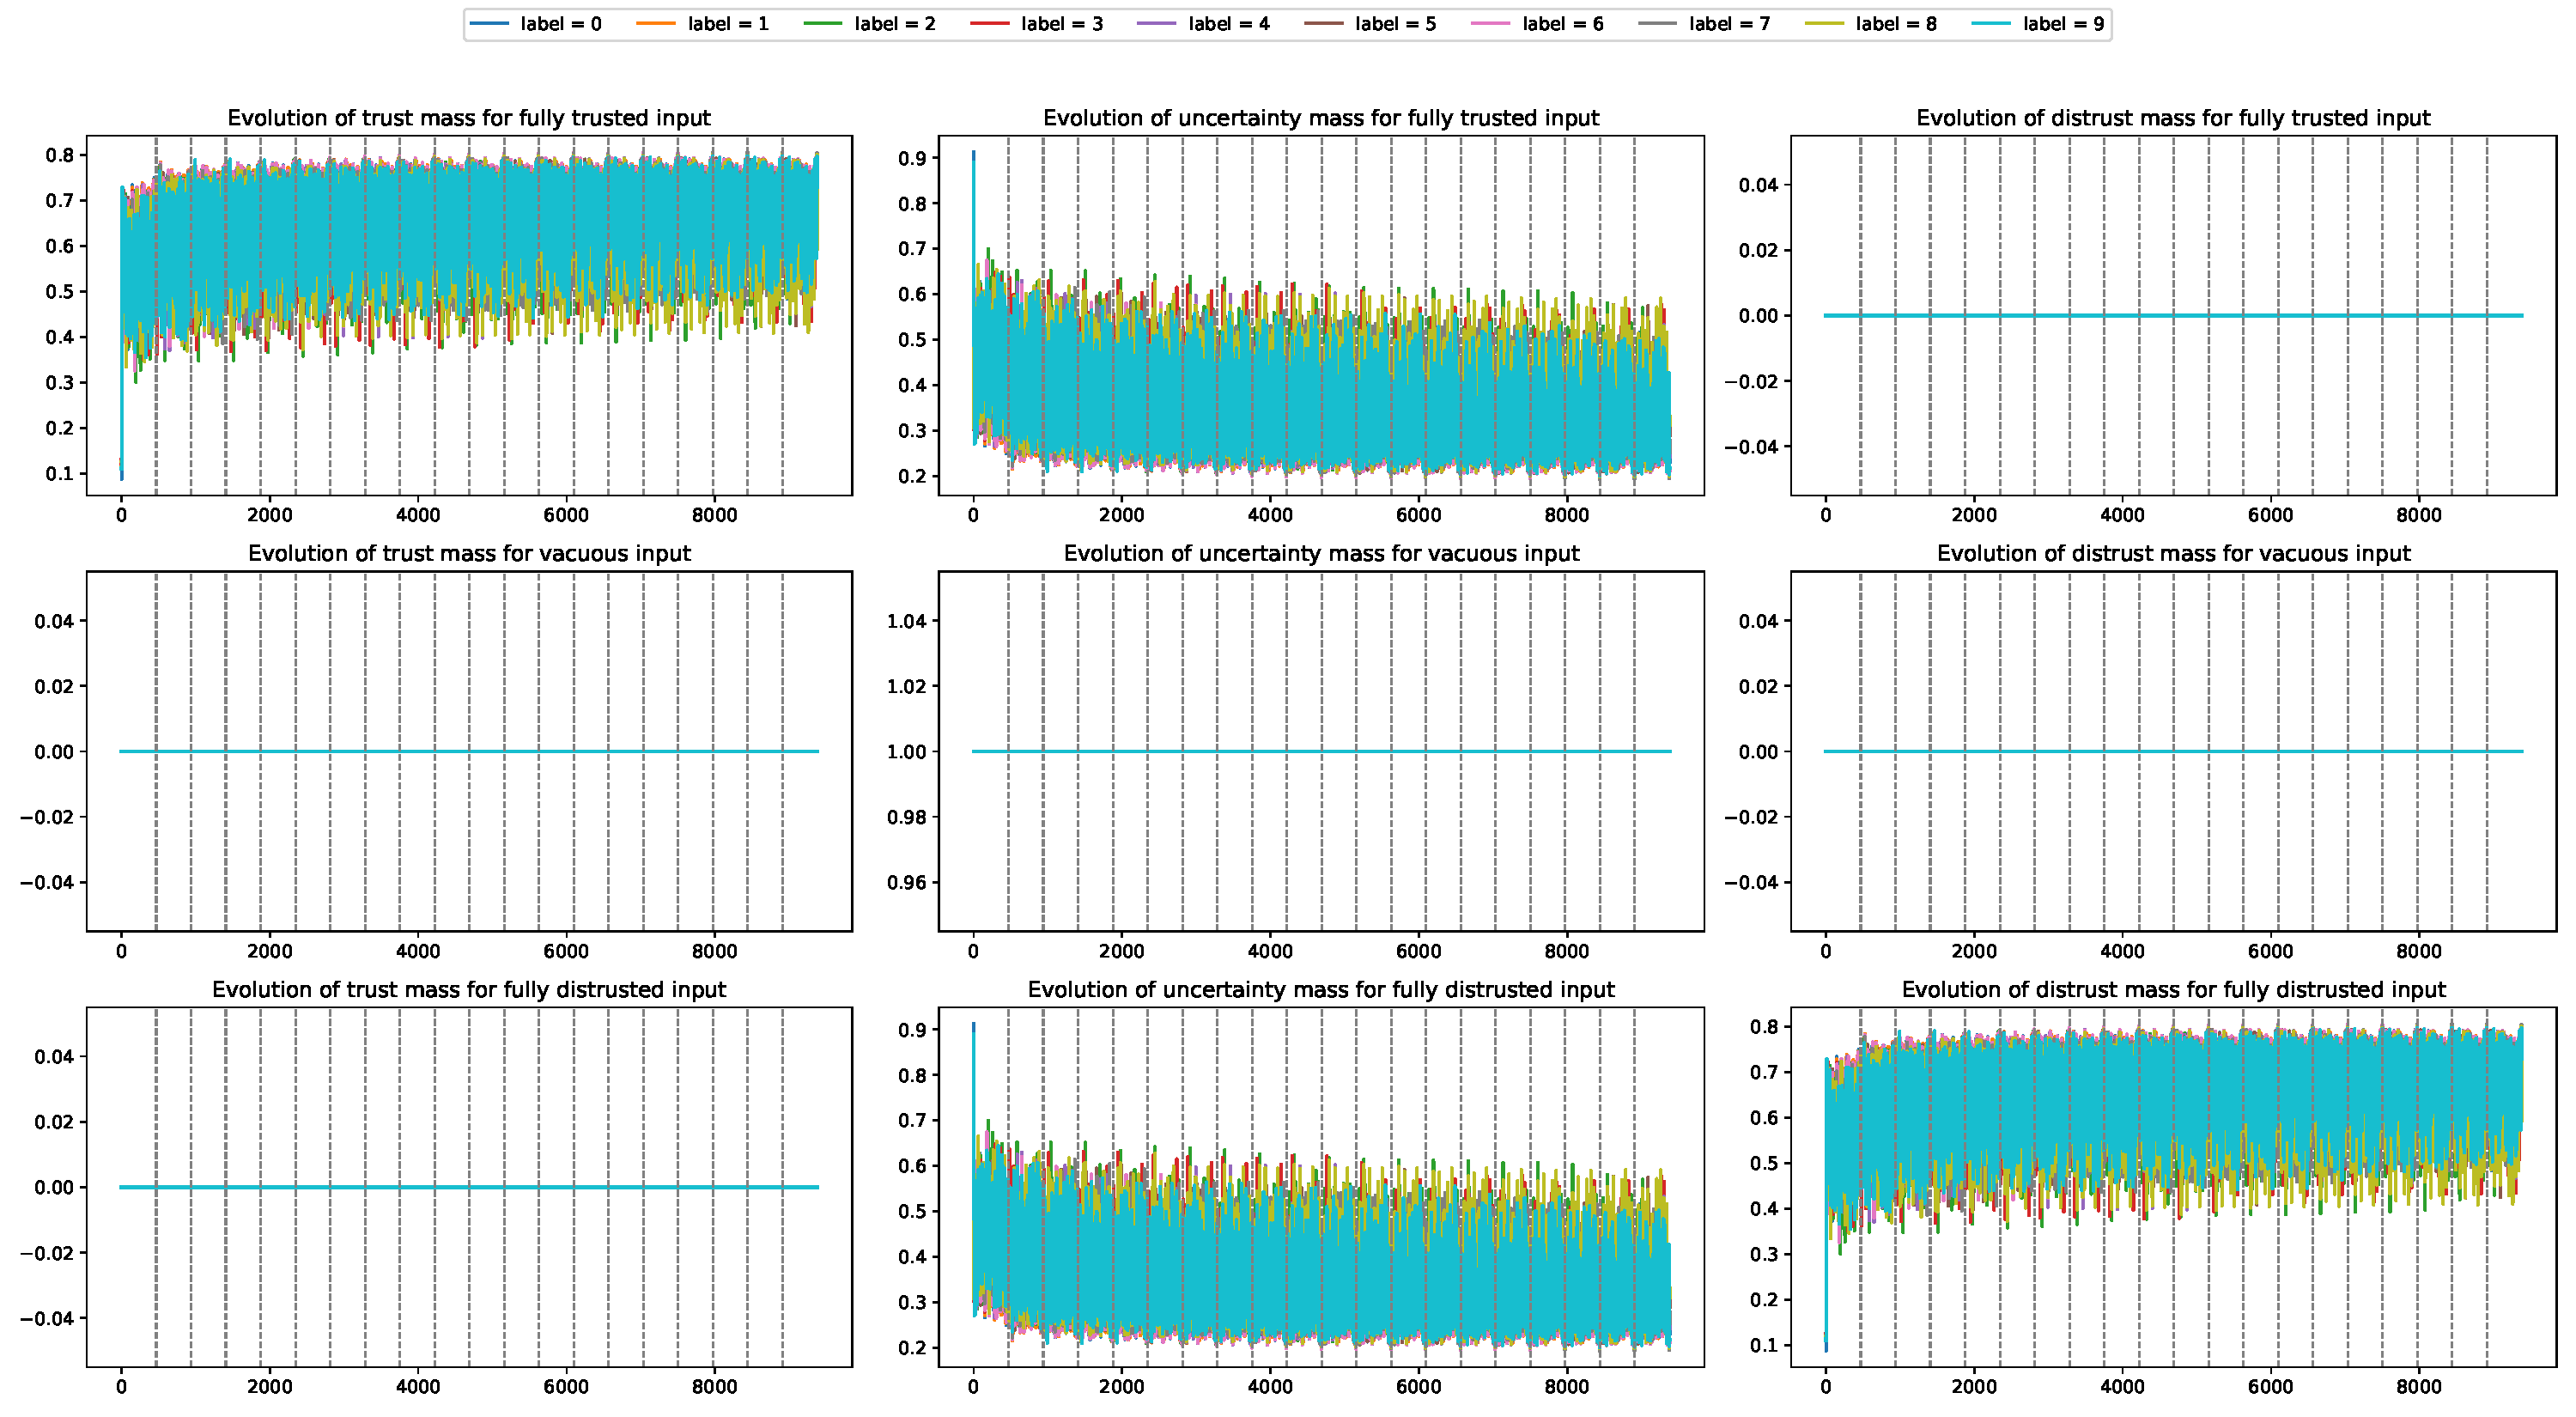
\includegraphics[width=0.8\textwidth]{latex/PTAS_Eval_mnist_16_16_trust_trust_eps_0.05_PathSize_None__plot_ptas.pdf}
\caption{mnist\_16\_16\_trust\_trust, $\varepsilon$=0.05}
\end{figure}

\begin{figure}[htbp]
\centering
  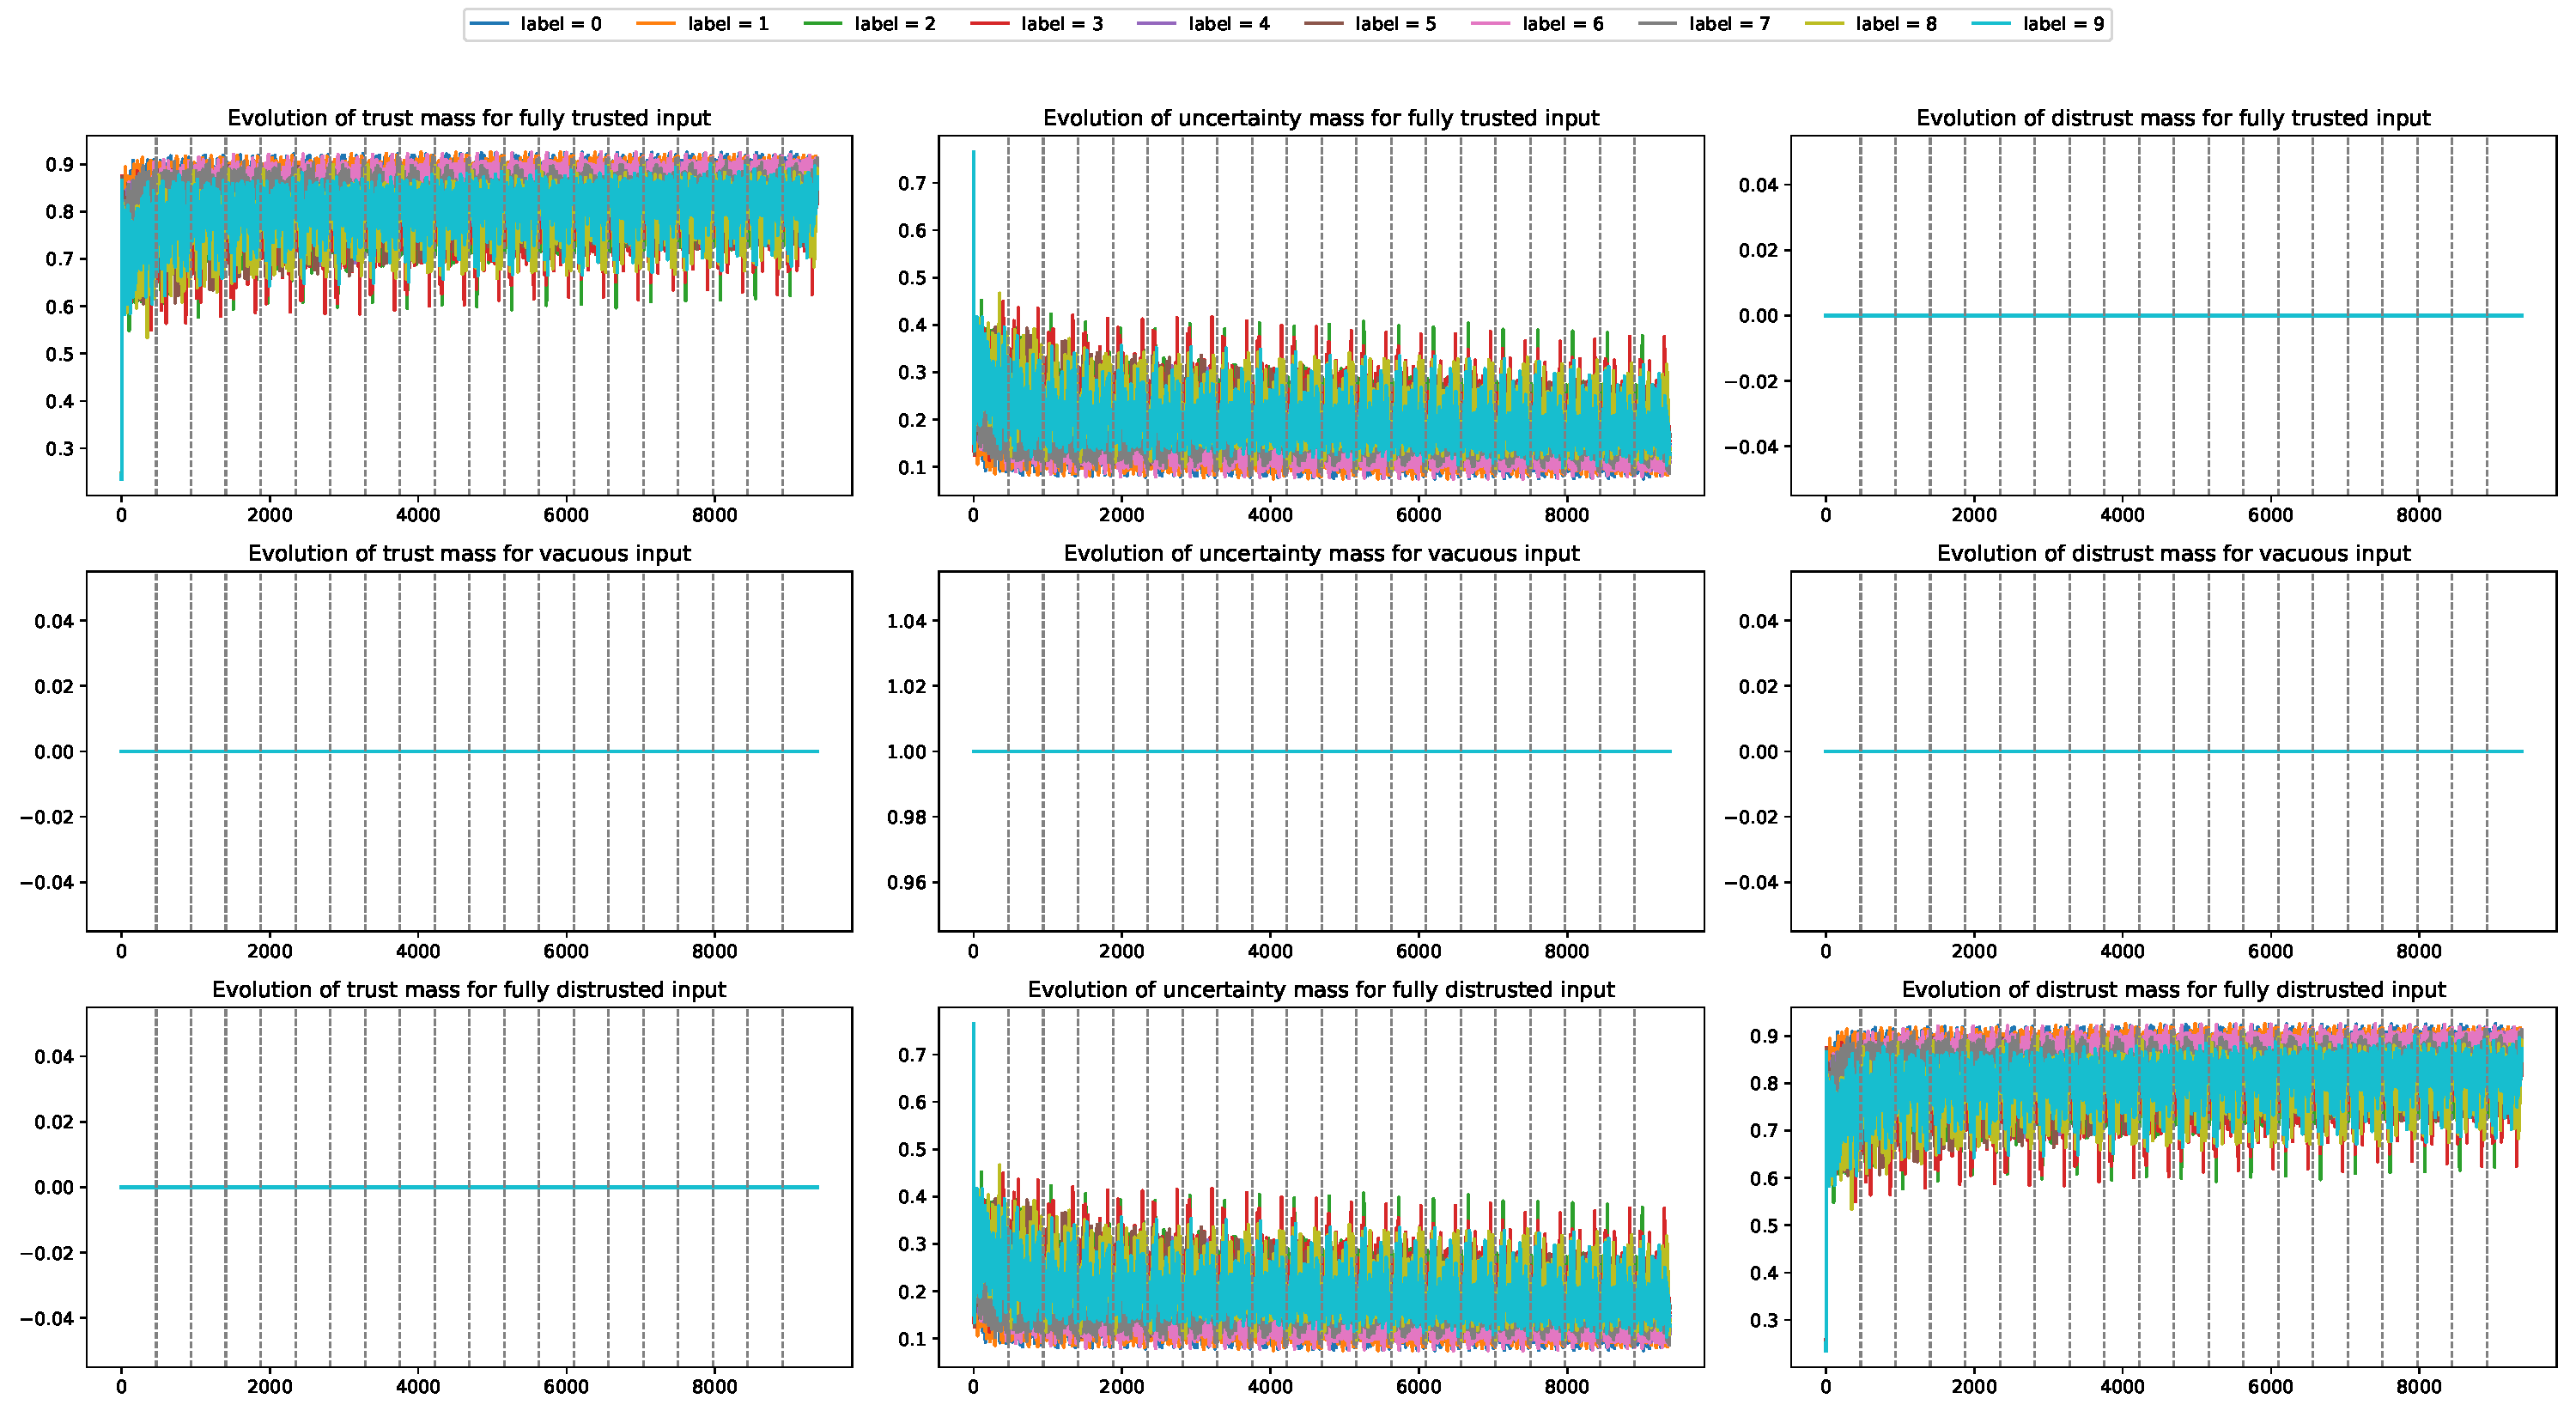
\includegraphics[width=0.8\textwidth]{latex/PTAS_Eval_mnist_16_trust_trust_eps_0.05_PathSize_None__plot_ptas.pdf}
\caption{mnist\_16\_trust\_trust, $\varepsilon$=0.05}
\end{figure}

\subsubsection{vacuous -- vacuous}

\begin{figure}[htbp]
\centering
  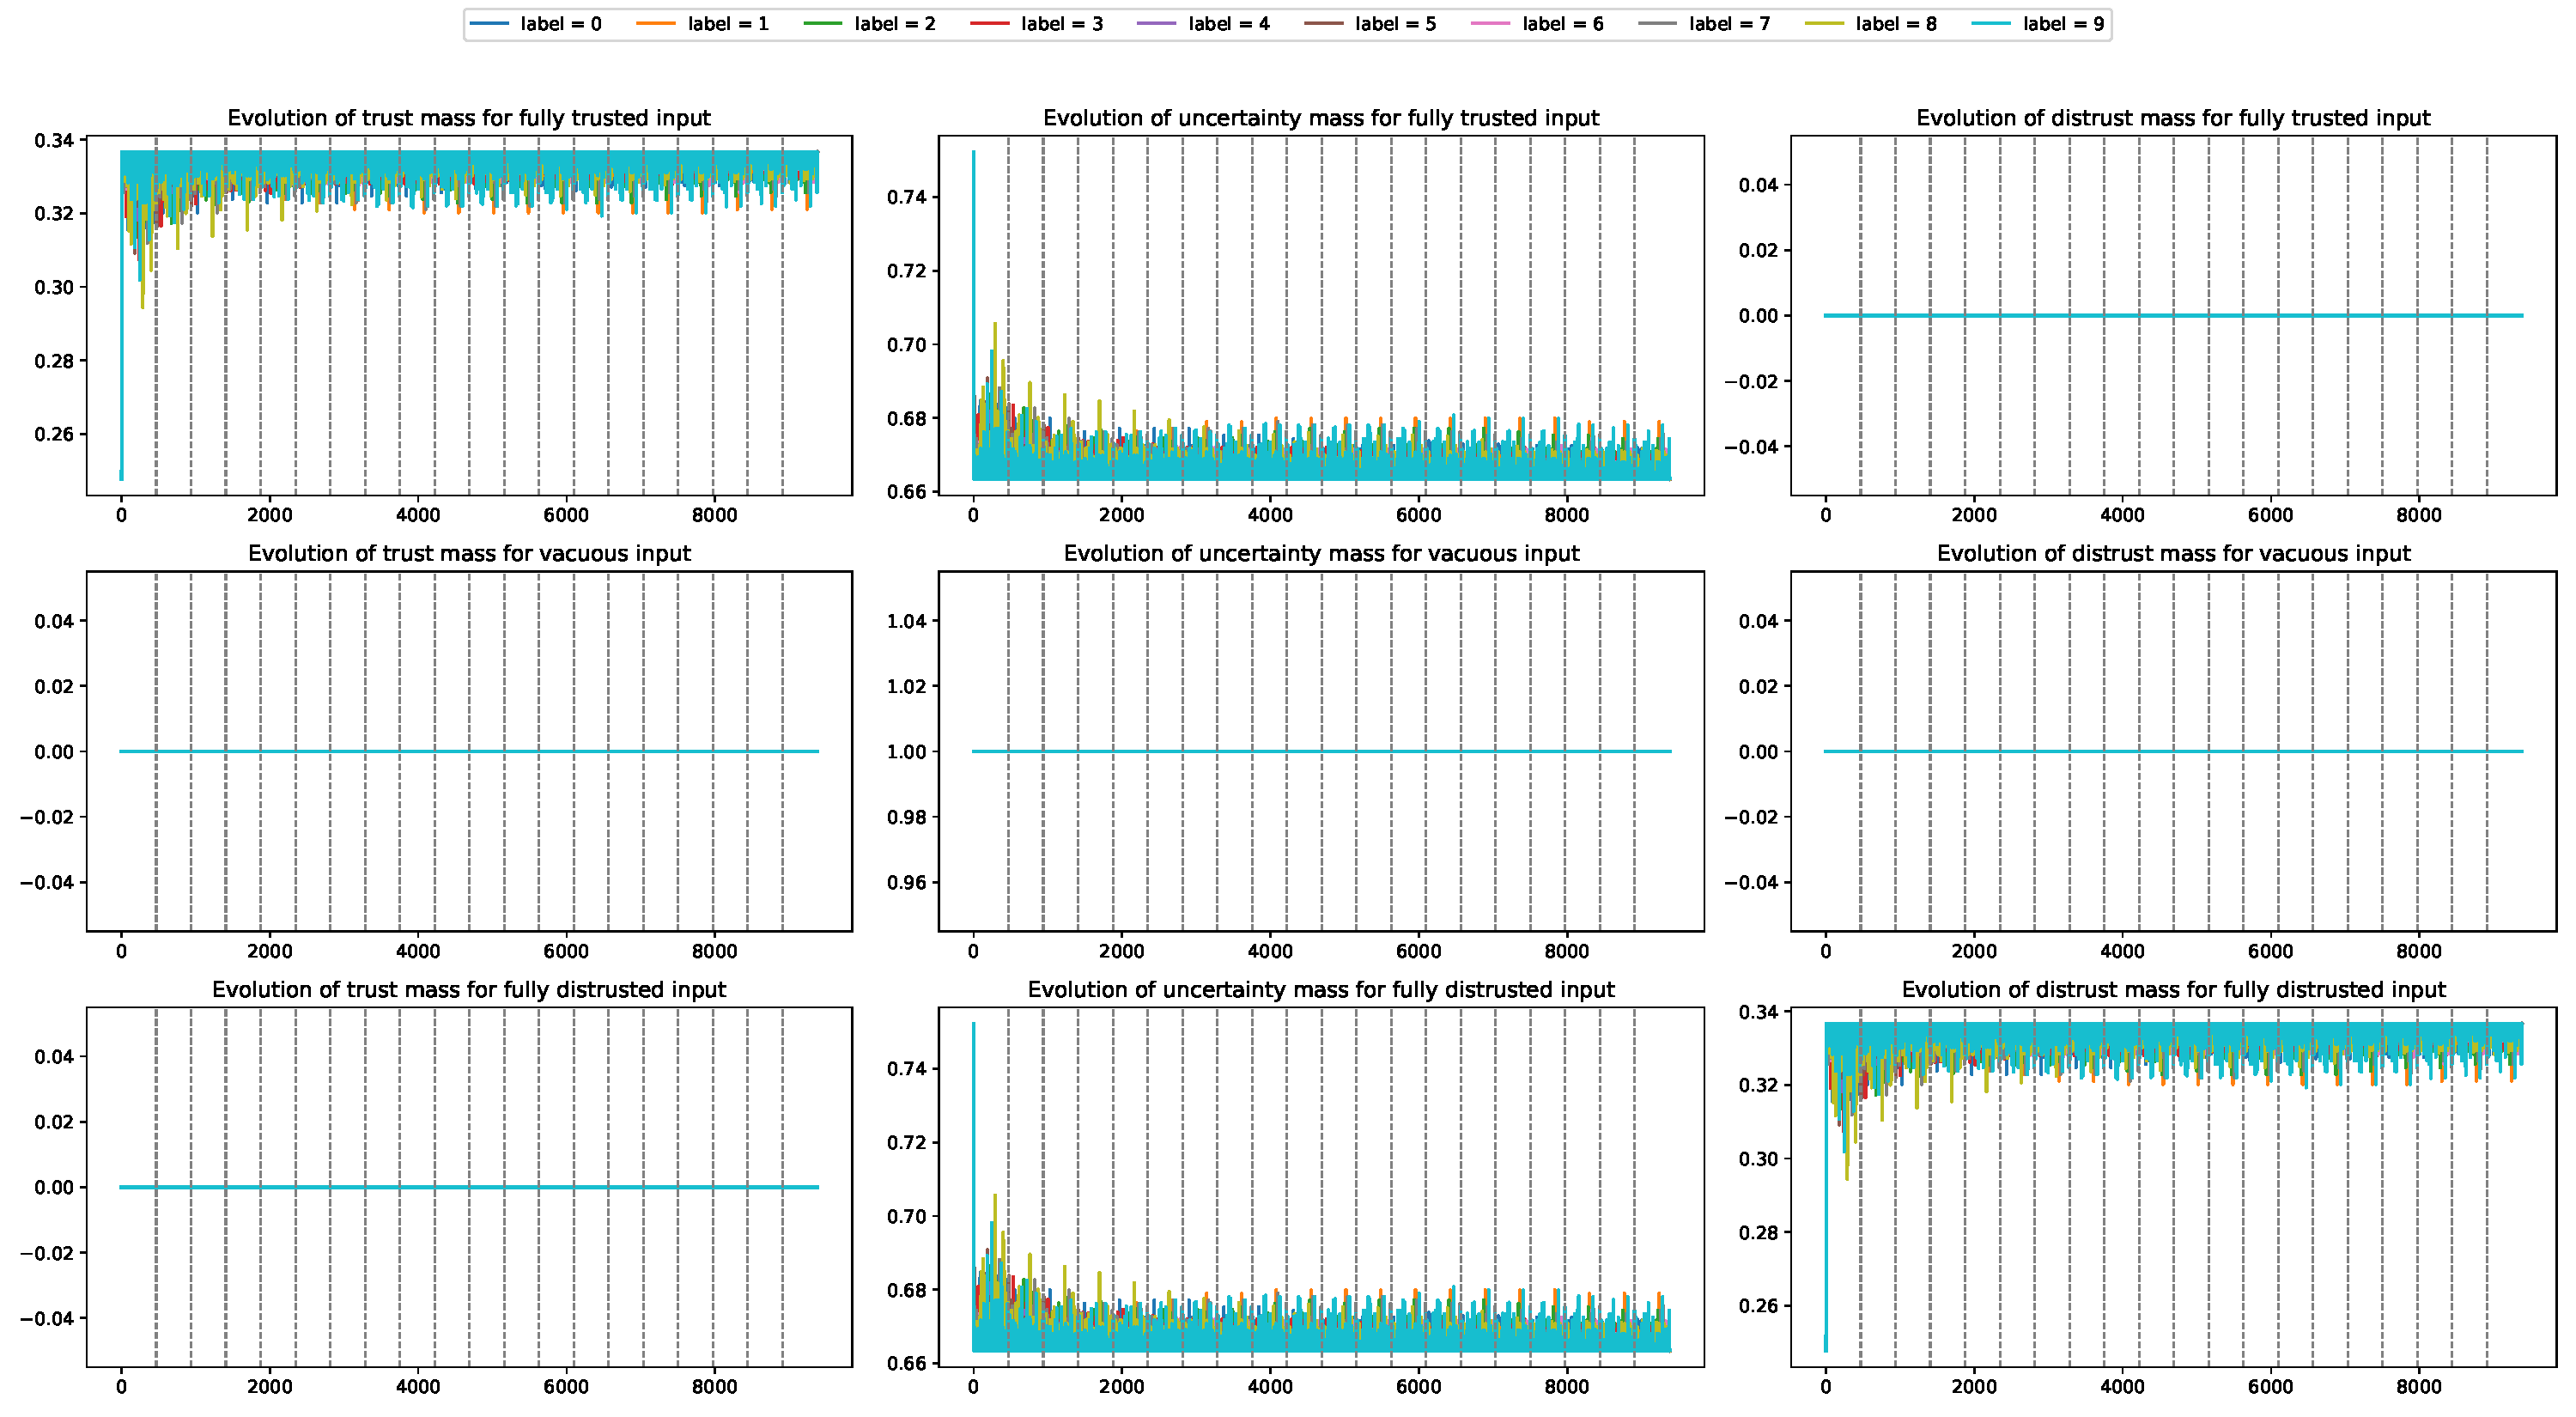
\includegraphics[width=0.8\textwidth]{latex/PTAS_Eval_mnist_128_vacuous_vacuous_eps_0.05_PathSize_None__plot_ptas.pdf}
\caption{mnist\_128\_vacuous\_vacuous, $\varepsilon$=0.05}
\end{figure}

\begin{figure}[htbp]
\centering
  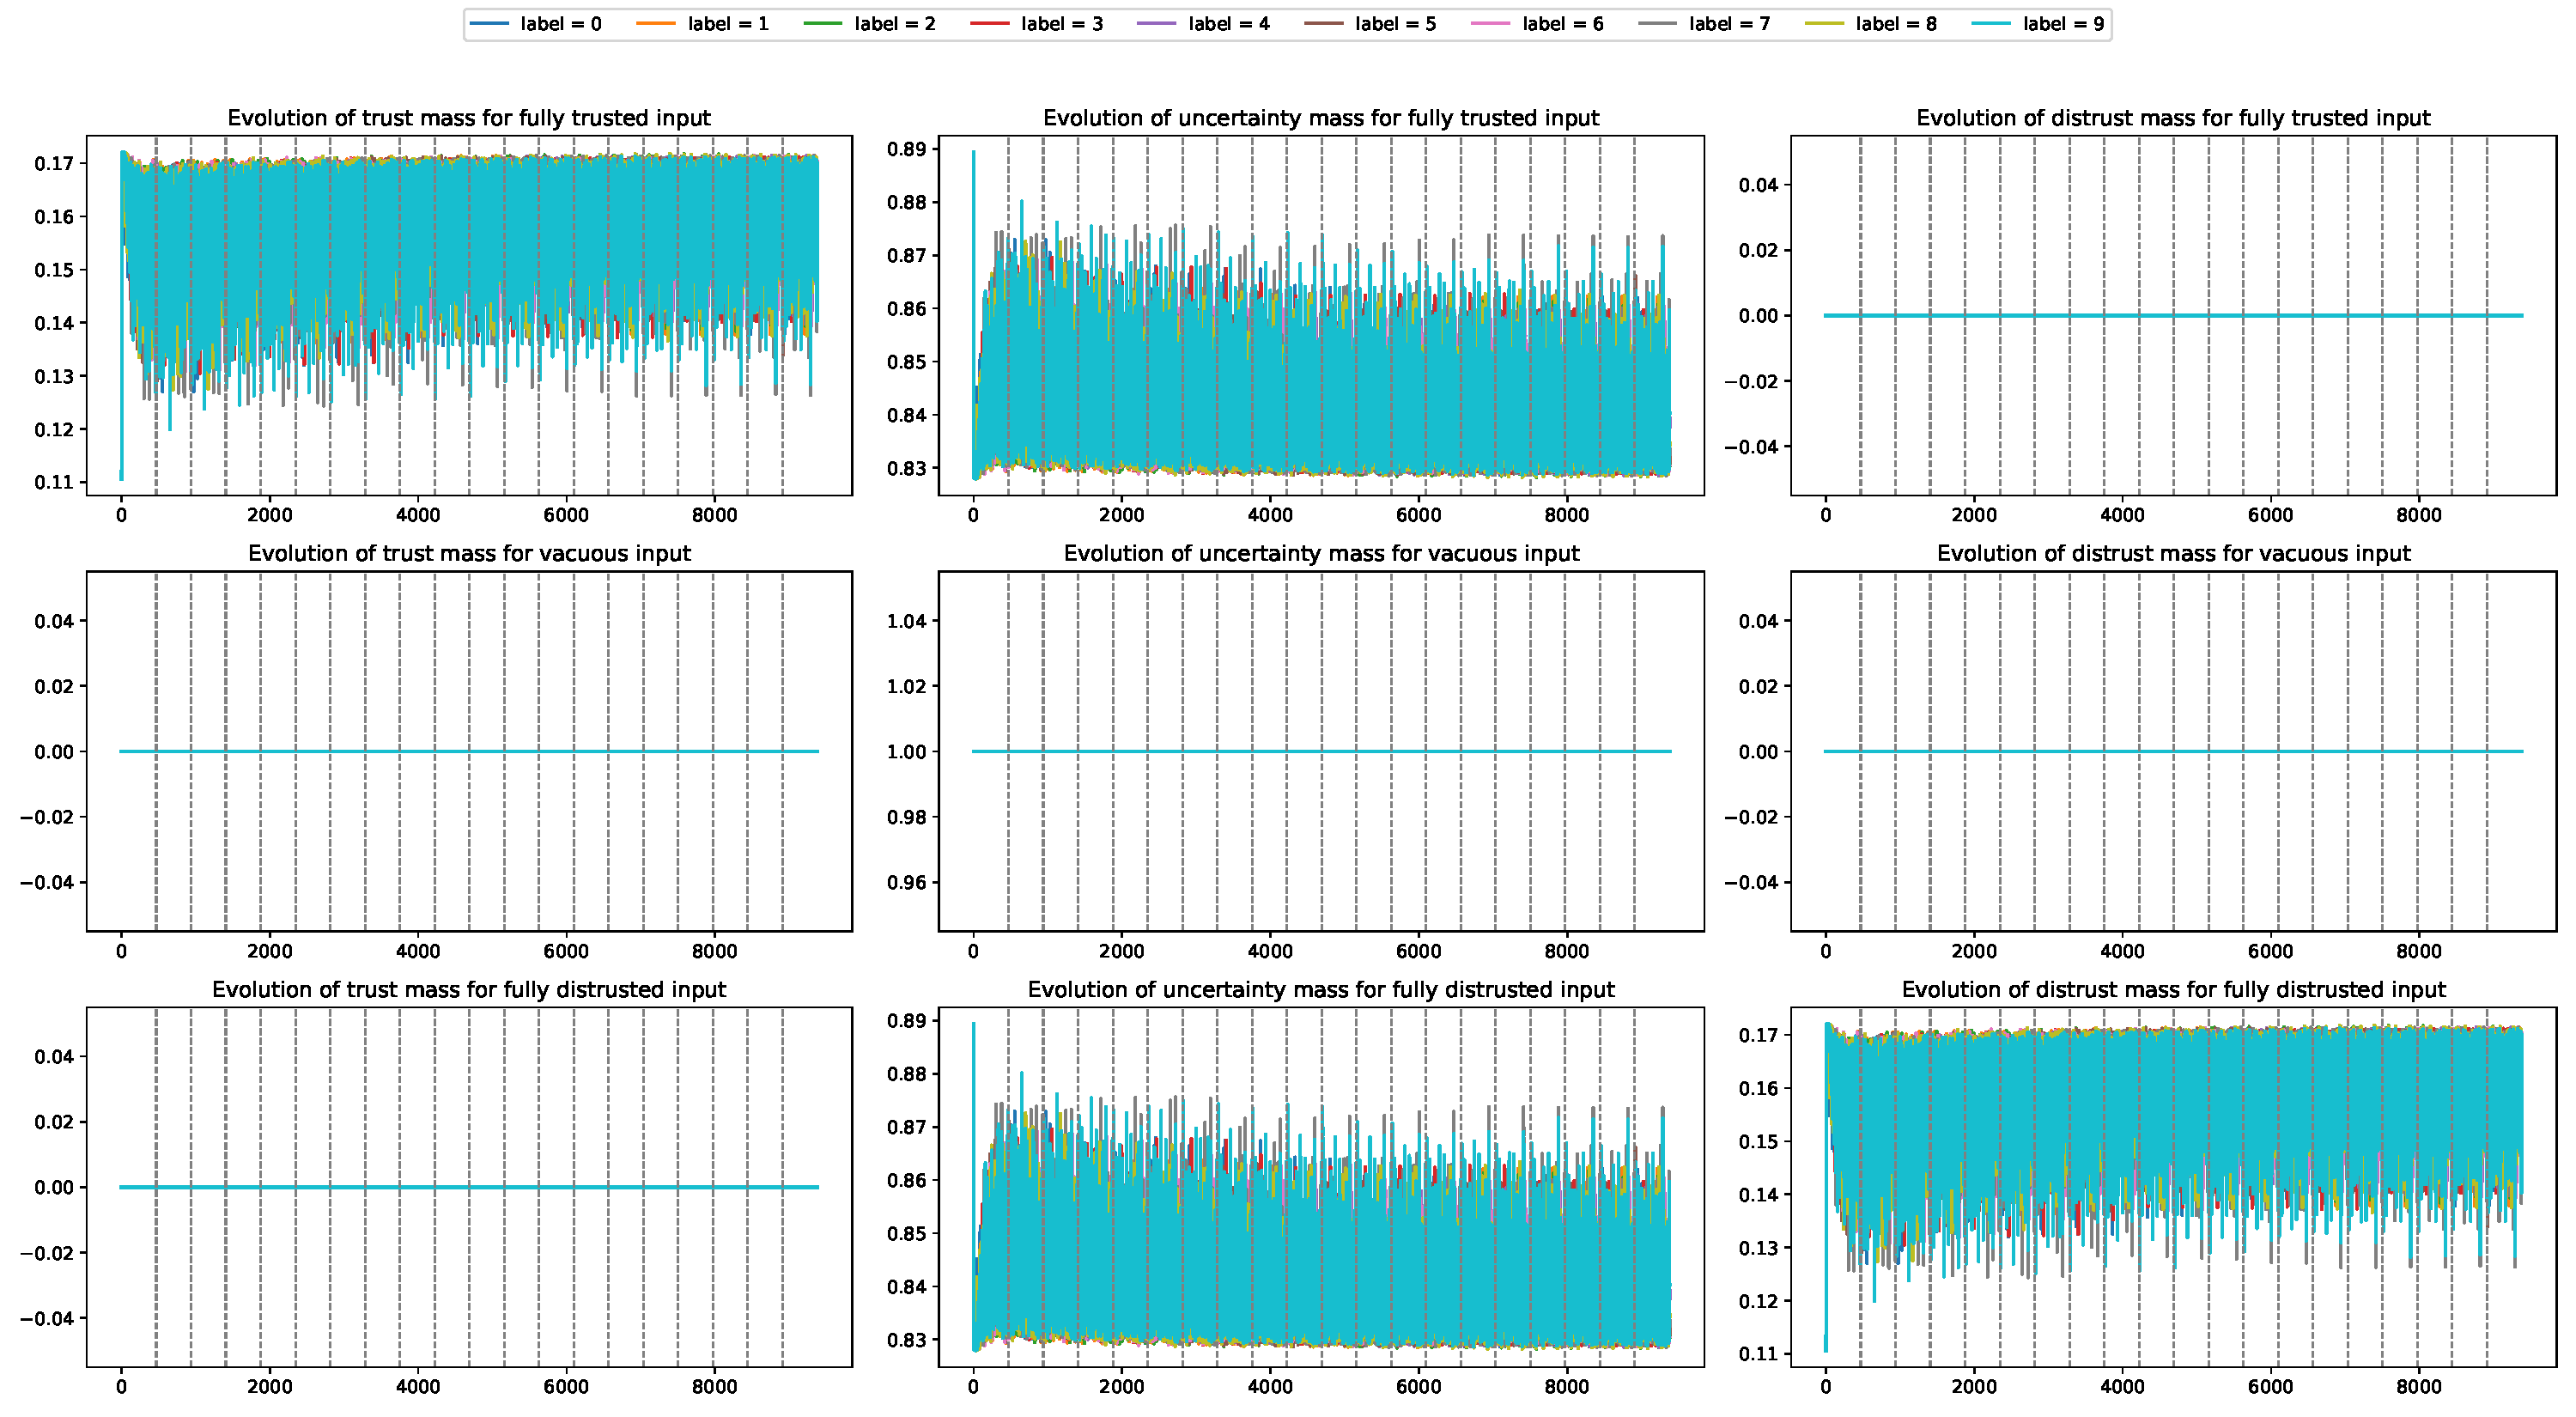
\includegraphics[width=0.8\textwidth]{latex/PTAS_Eval_mnist_16_16_vacuous_vacuous_eps_0.05_PathSize_None__plot_ptas.pdf}
\caption{mnist\_16\_16\_vacuous\_vacuous, $\varepsilon$=0.05}
\end{figure}

\begin{figure}[htbp]
\centering
  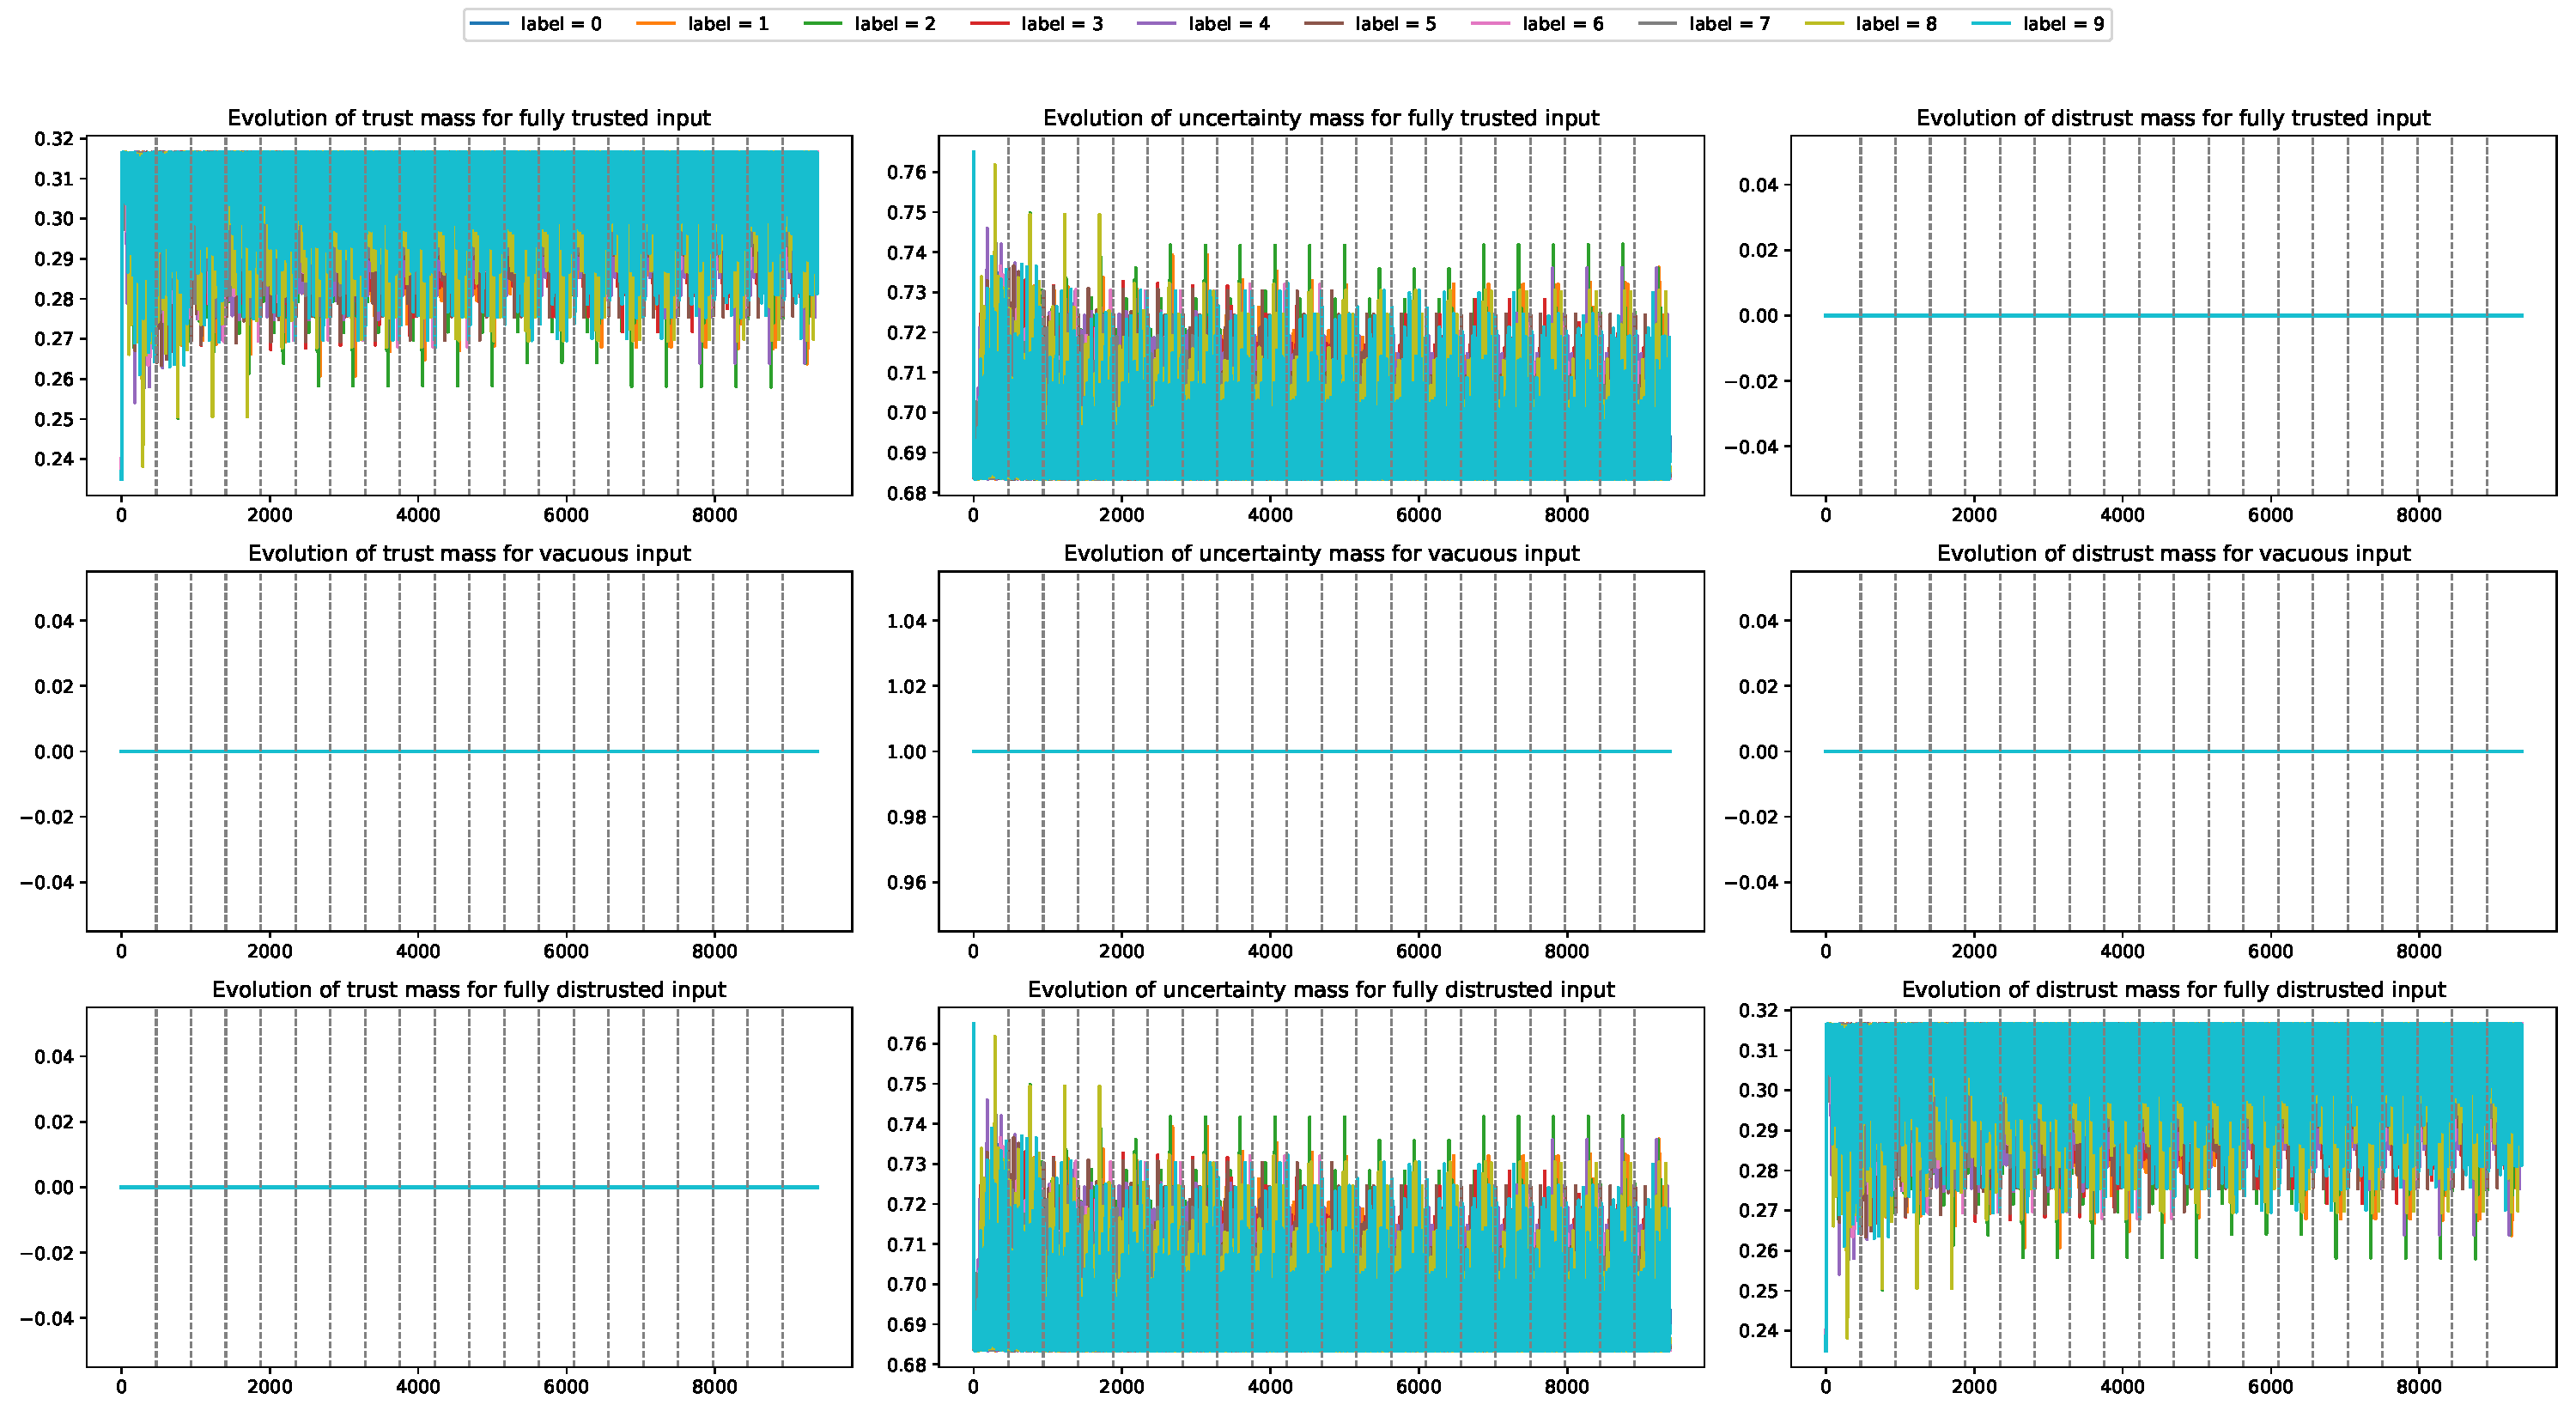
\includegraphics[width=0.8\textwidth]{latex/PTAS_Eval_mnist_16_vacuous_vacuous_eps_0.05_PathSize_None__plot_ptas.pdf}
\caption{mnist\_16\_vacuous\_vacuous, $\varepsilon$=0.05}
\end{figure}

\begin{figure}[htbp]
\centering
  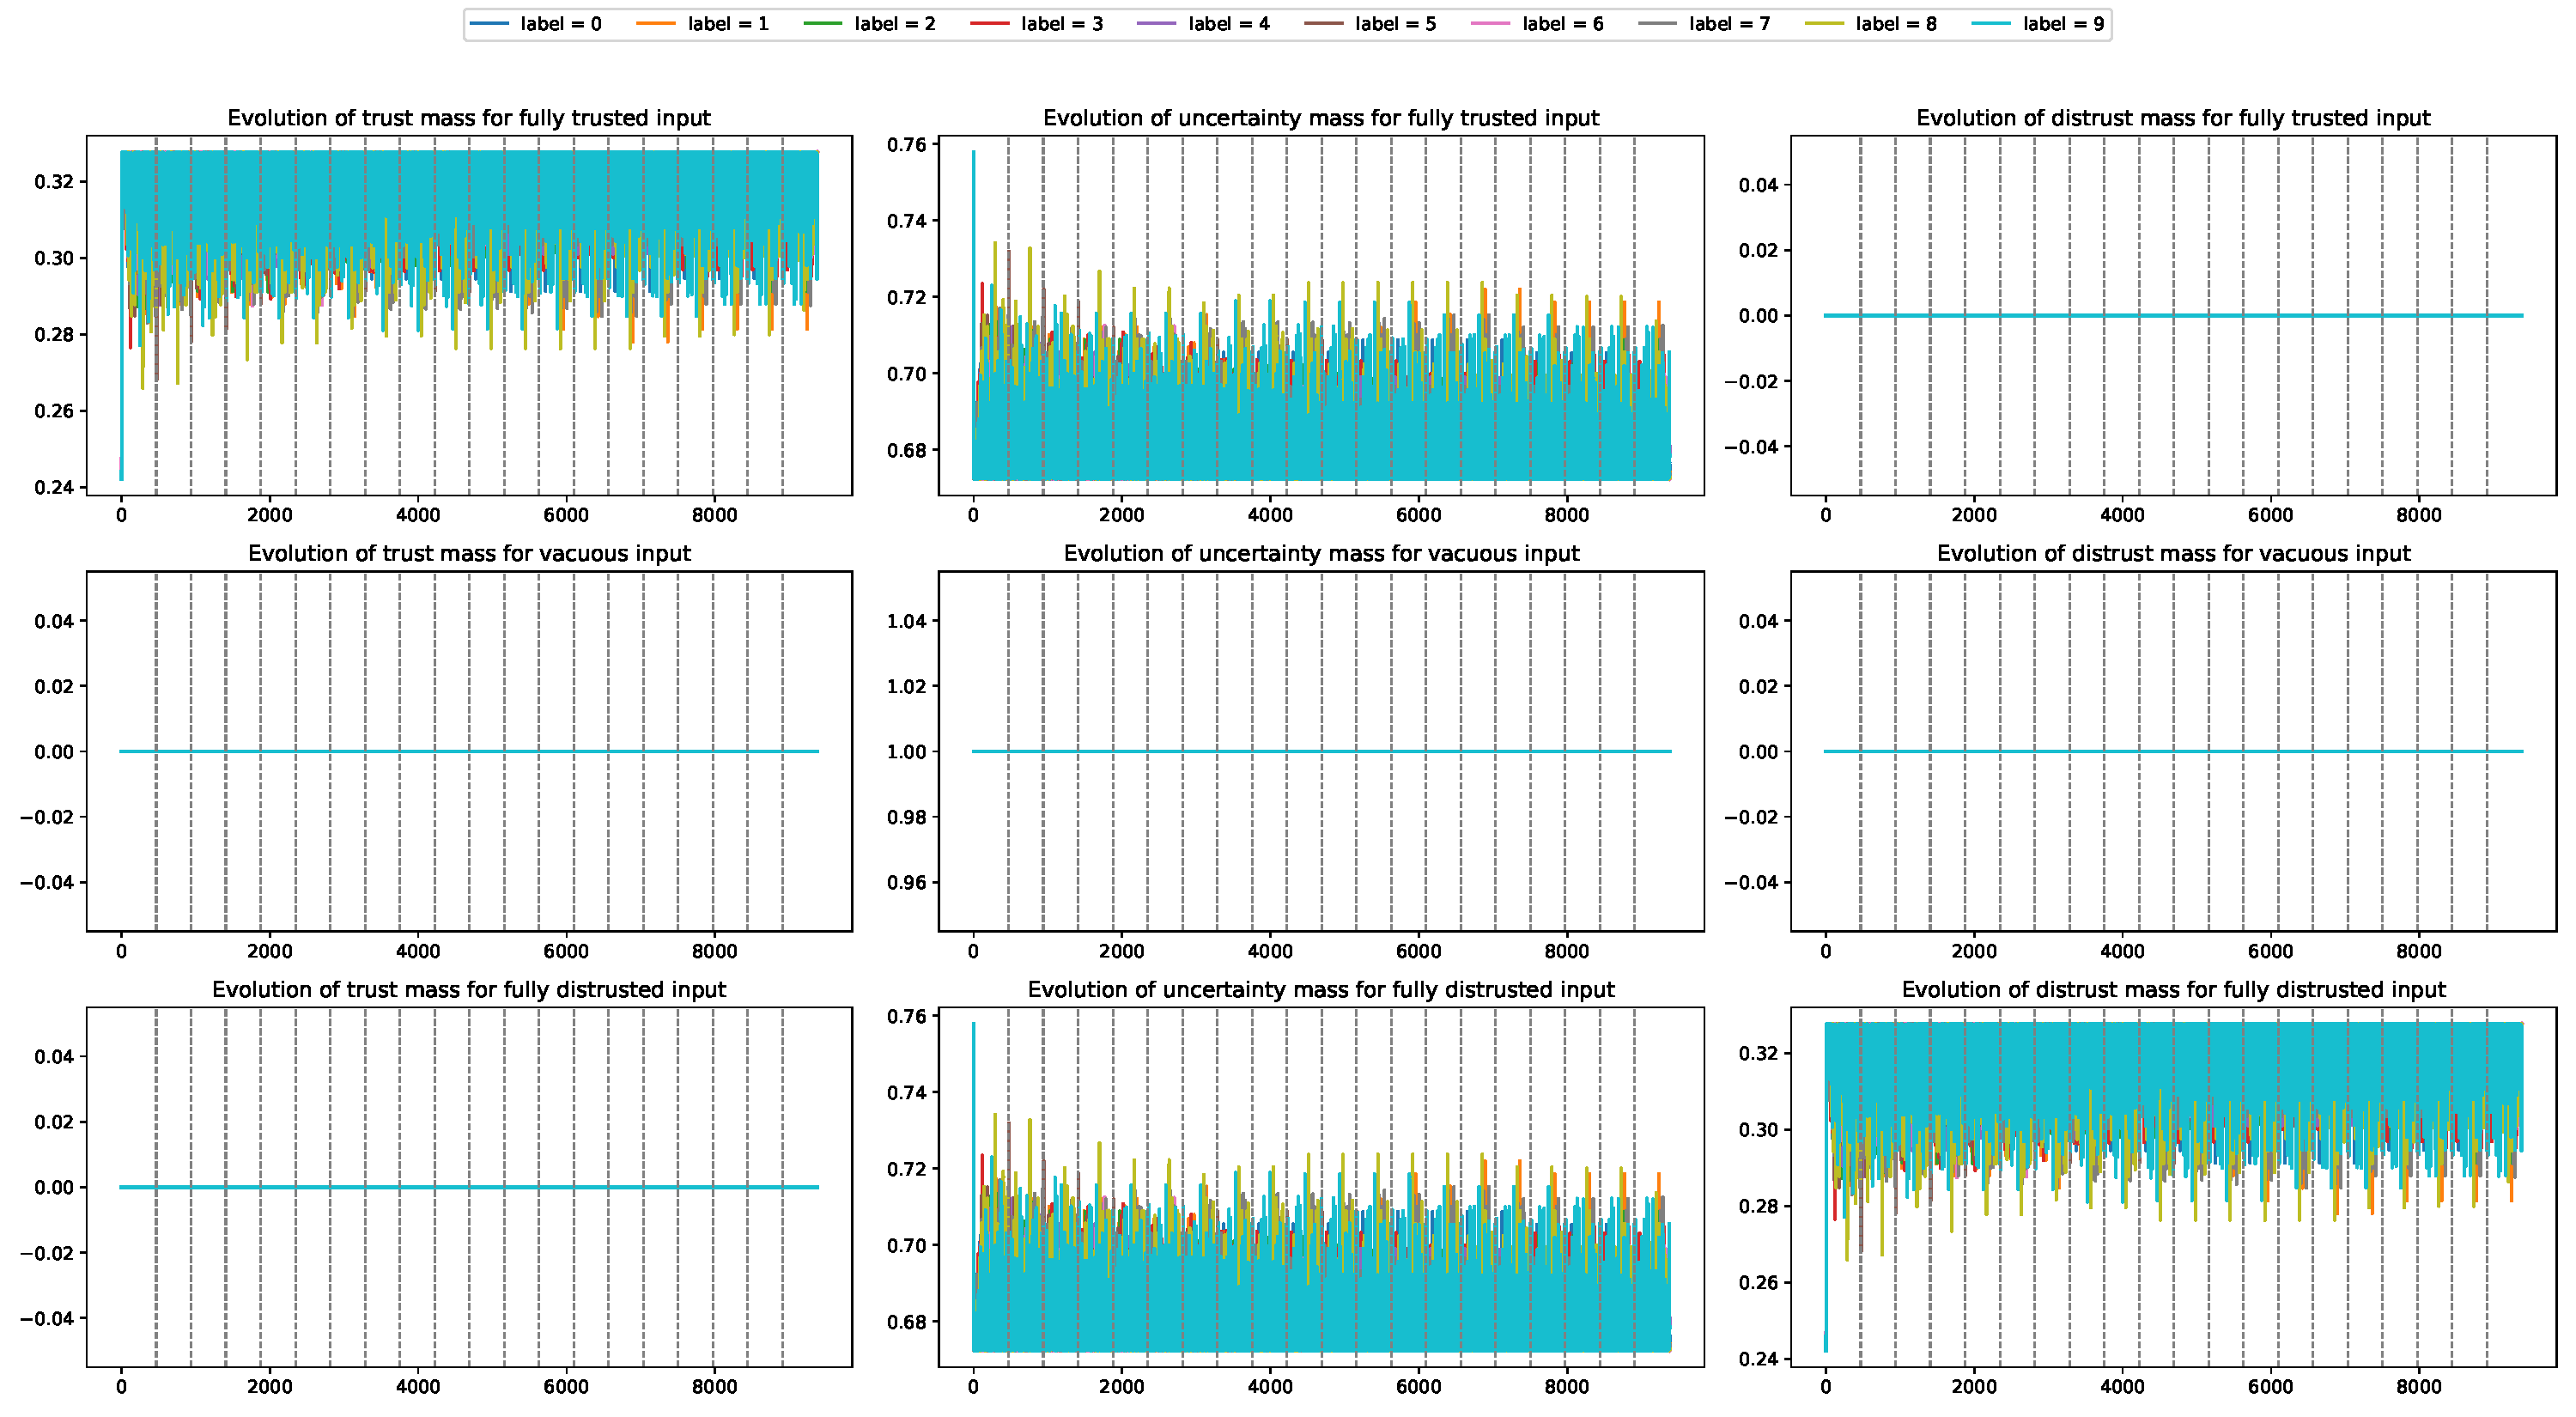
\includegraphics[width=0.8\textwidth]{latex/PTAS_Eval_mnist_32_vacuous_vacuous_eps_0.05_PathSize_None__plot_ptas.pdf}
\caption{mnist\_32\_vacuous\_vacuous, $\varepsilon$=0.05}
\end{figure}

\begin{figure}[htbp]
\centering
  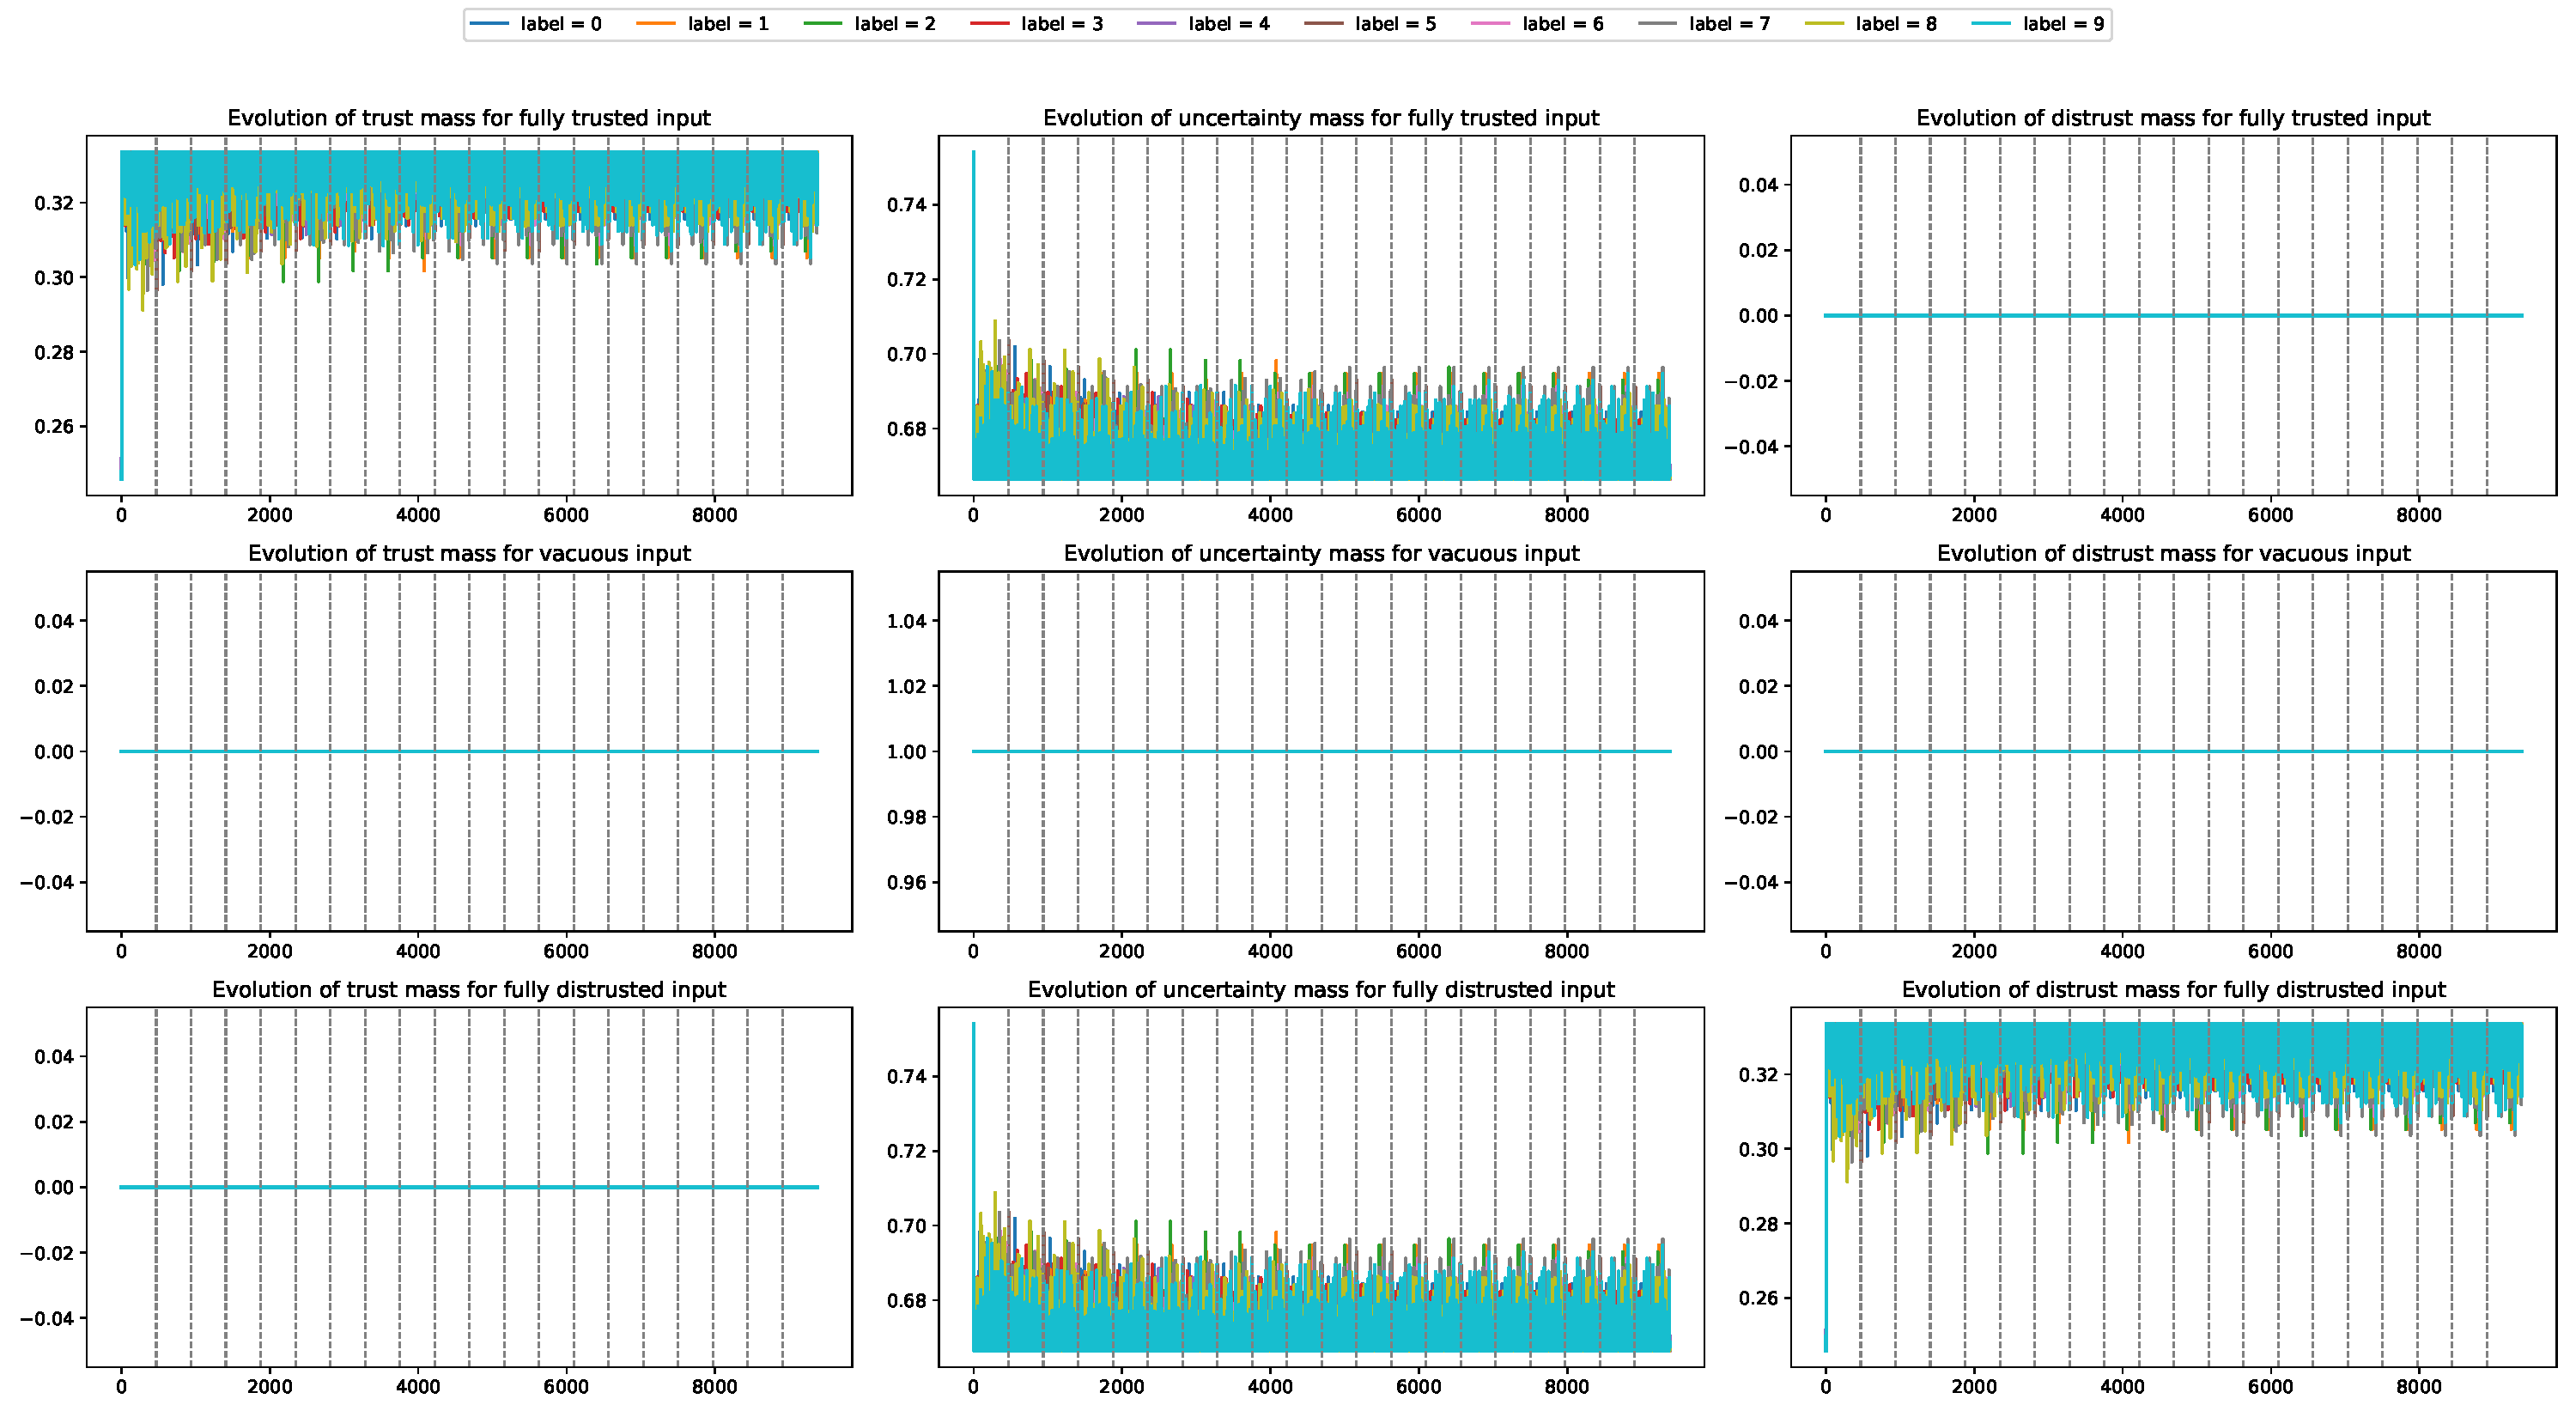
\includegraphics[width=0.8\textwidth]{latex/PTAS_Eval_mnist_64_vacuous_vacuous_eps_0.05_PathSize_None__plot_ptas.pdf}
\caption{mnist\_64\_vacuous\_vacuous, $\varepsilon$=0.05}
\end{figure}

\subsection{\ac{IPTA}}

\begin{figure}[htbp]
\centering
\subfloat[{mnist\_128\_trust\_trust, ps=1}]{%
  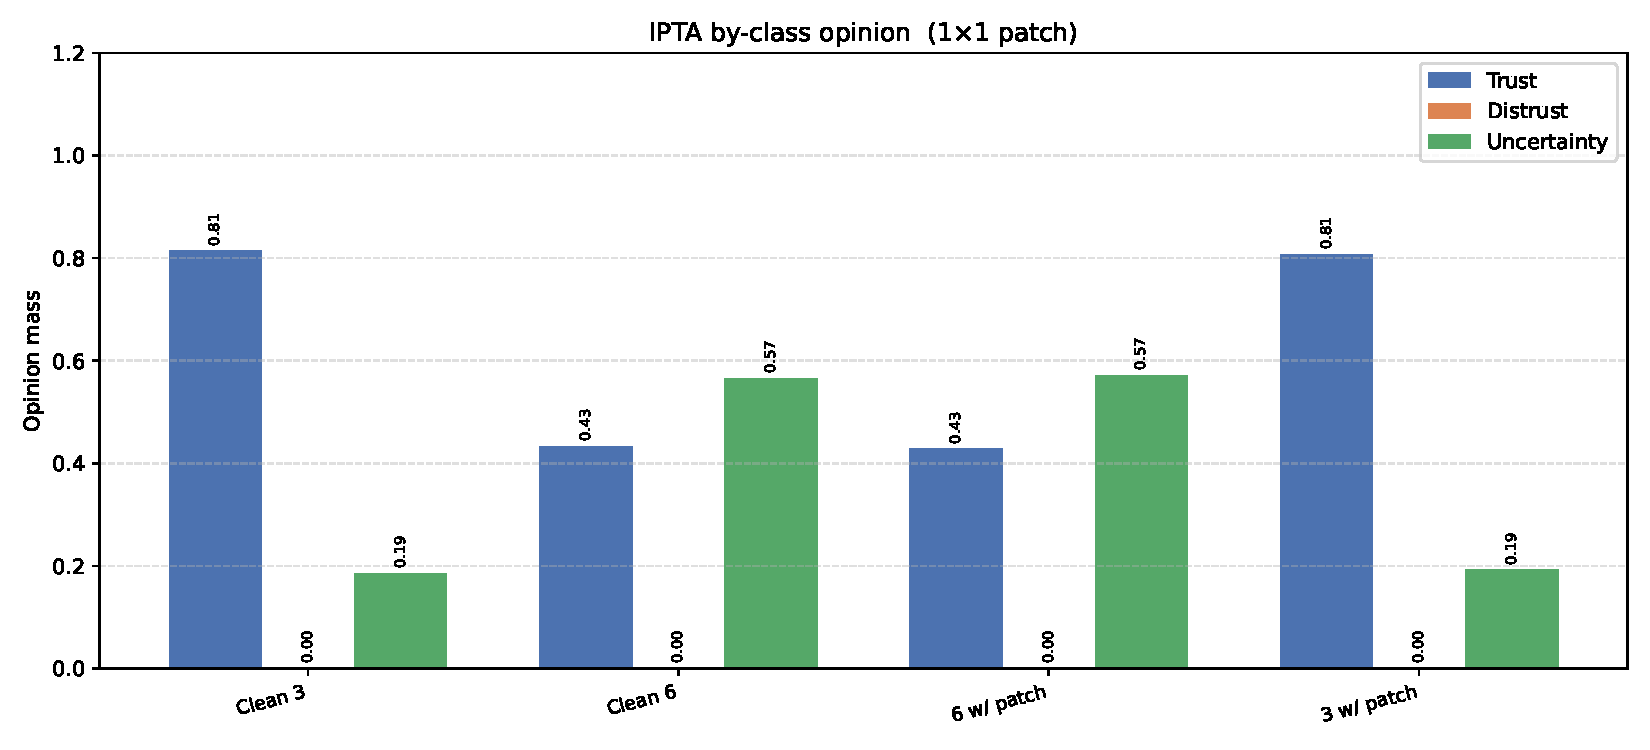
\includegraphics[width=0.3\textwidth]{latex/NN_Train_mnist_128_trust_trust_PathSize_1__ipta_table2a.pdf}%
}
\subfloat[{mnist\_128\_trust\_trust, ps=10}]{%
  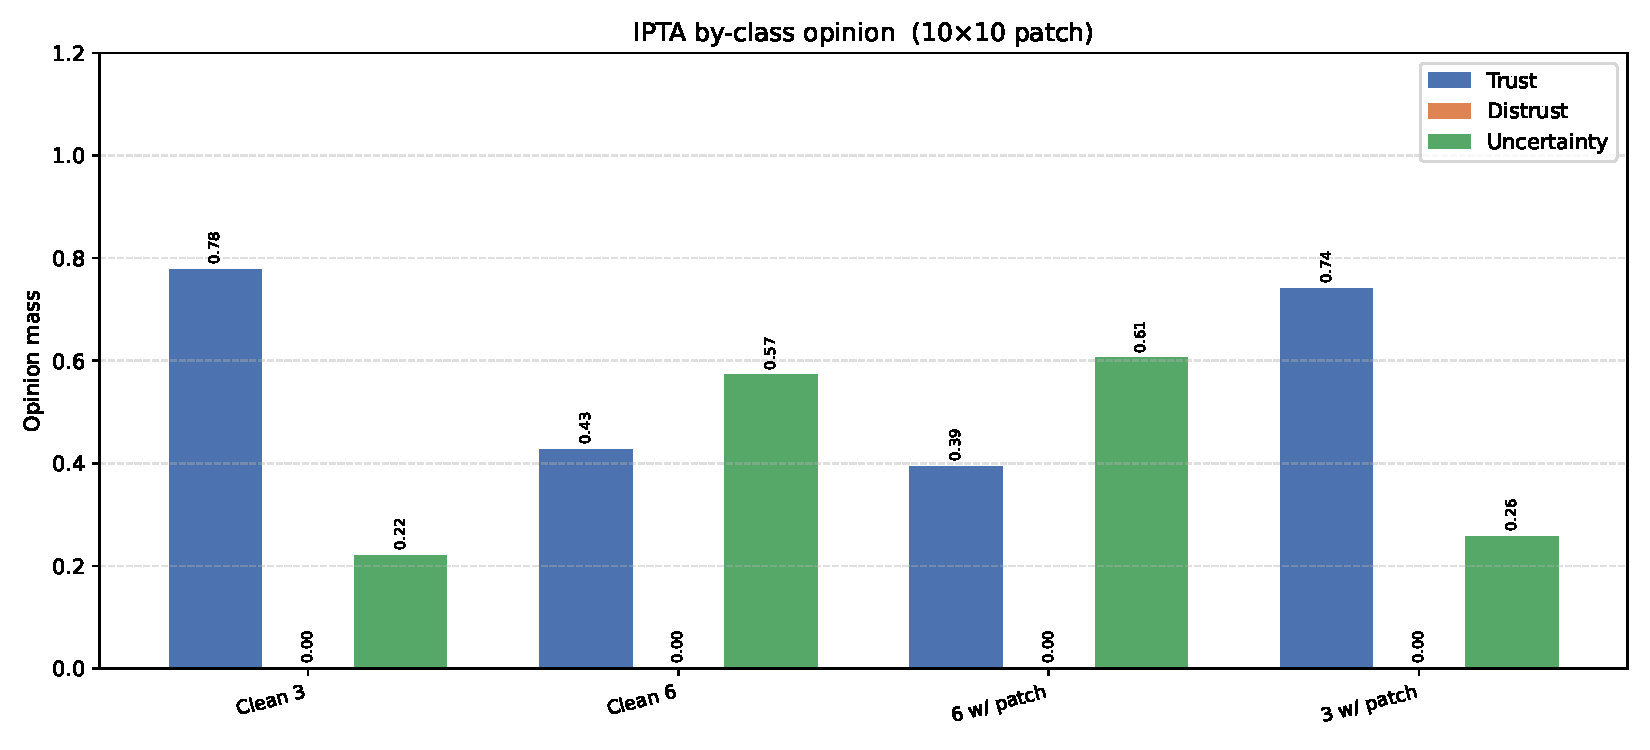
\includegraphics[width=0.3\textwidth]{latex/NN_Train_mnist_128_trust_trust_PathSize_10__ipta_table2a.pdf}%
}
\subfloat[{mnist\_128\_trust\_trust, ps=27}]{%
  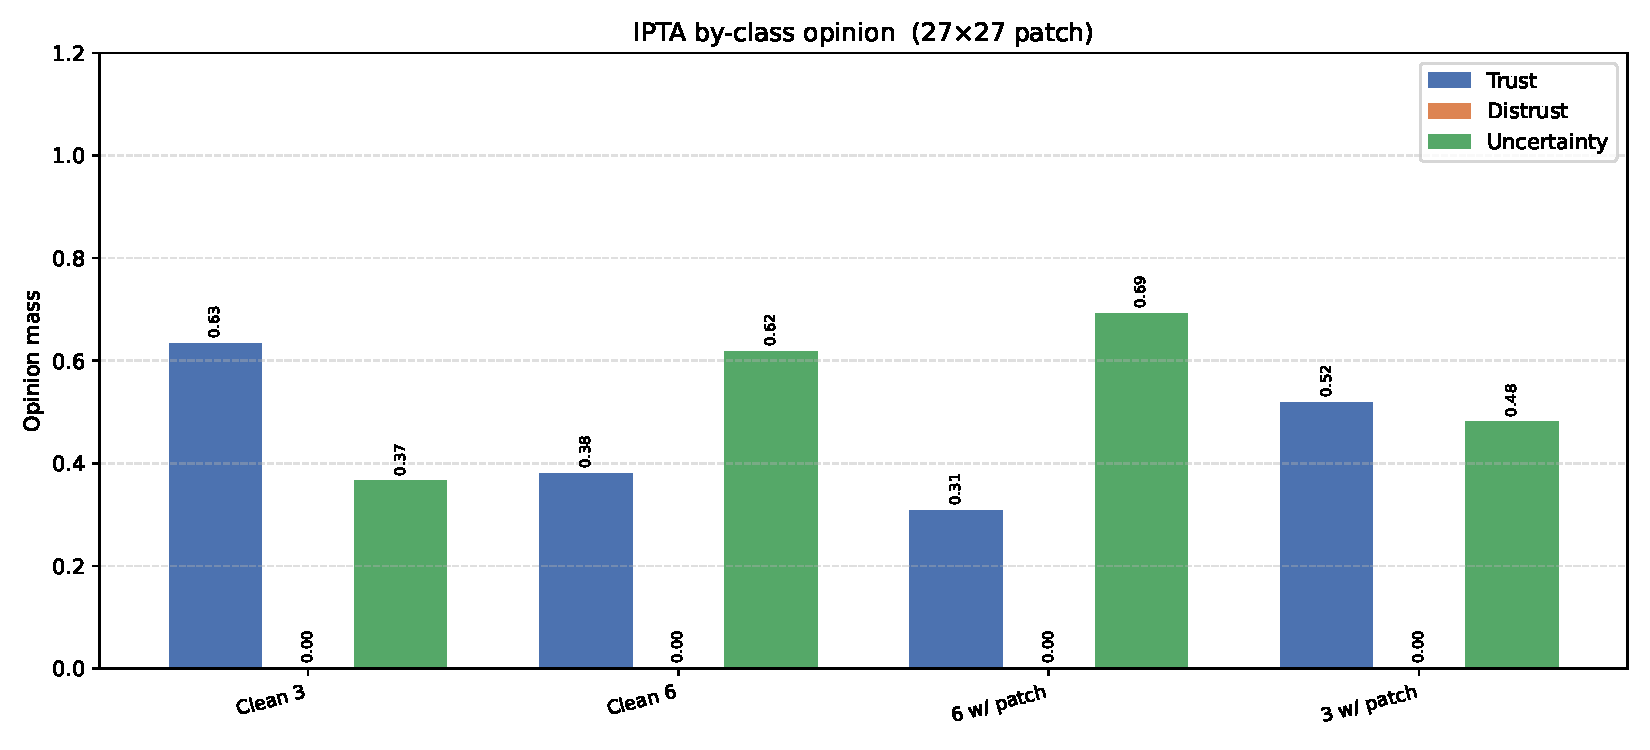
\includegraphics[width=0.3\textwidth]{latex/NN_Train_mnist_128_trust_trust_PathSize_27__ipta_table2a.pdf}%
}
\\
\subfloat[{mnist\_128\_trust\_trust, ps=4}]{%
  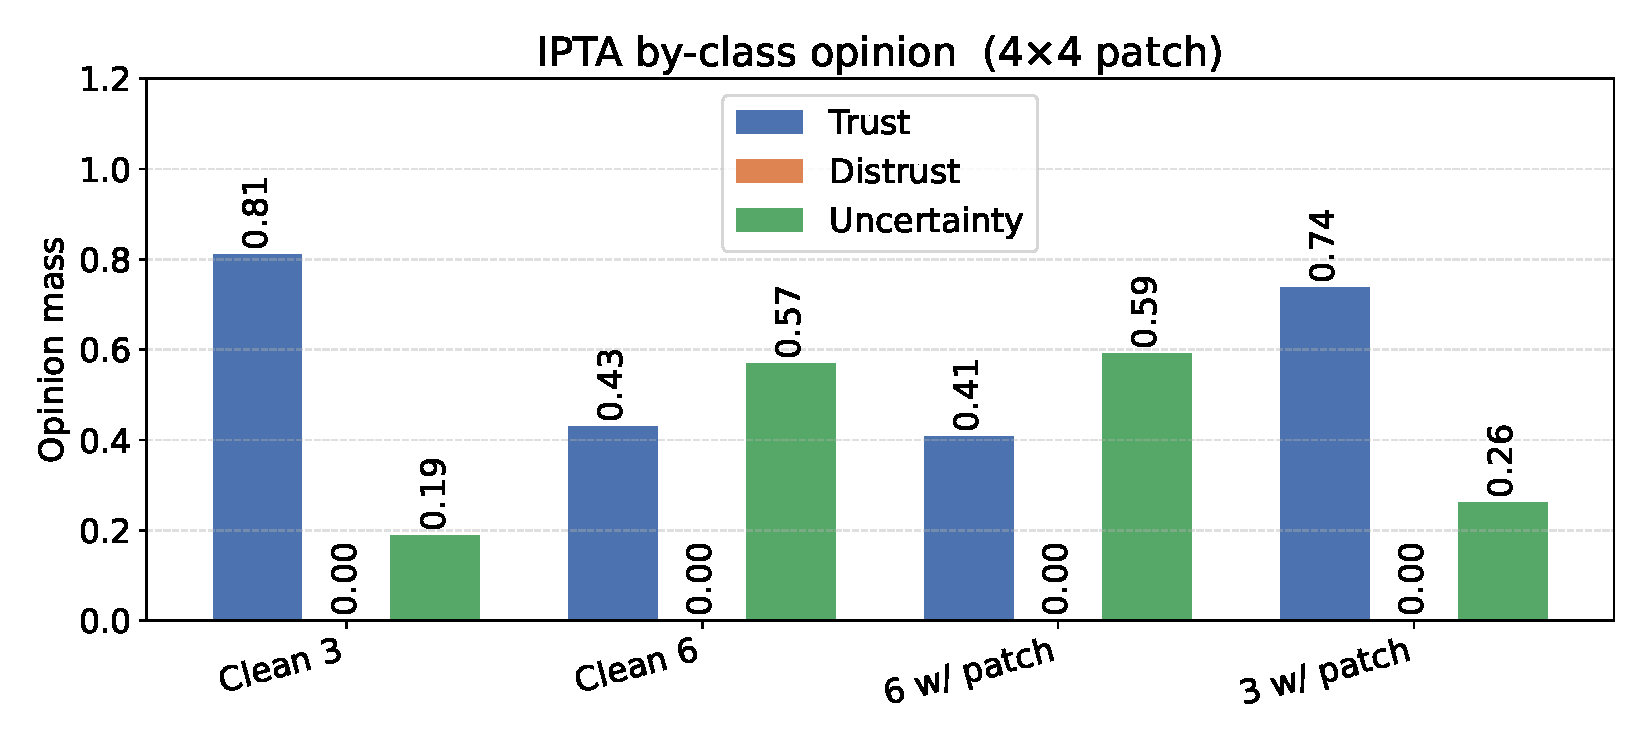
\includegraphics[width=0.3\textwidth]{latex/NN_Train_mnist_128_trust_trust_PathSize_4__ipta_table2a.pdf}%
}
\caption{IPTA -- Table 2a}
\end{figure}


\begin{figure}[htbp]
\centering
\subfloat[{mnist\_128\_trust\_trust, ps=1}]{%
  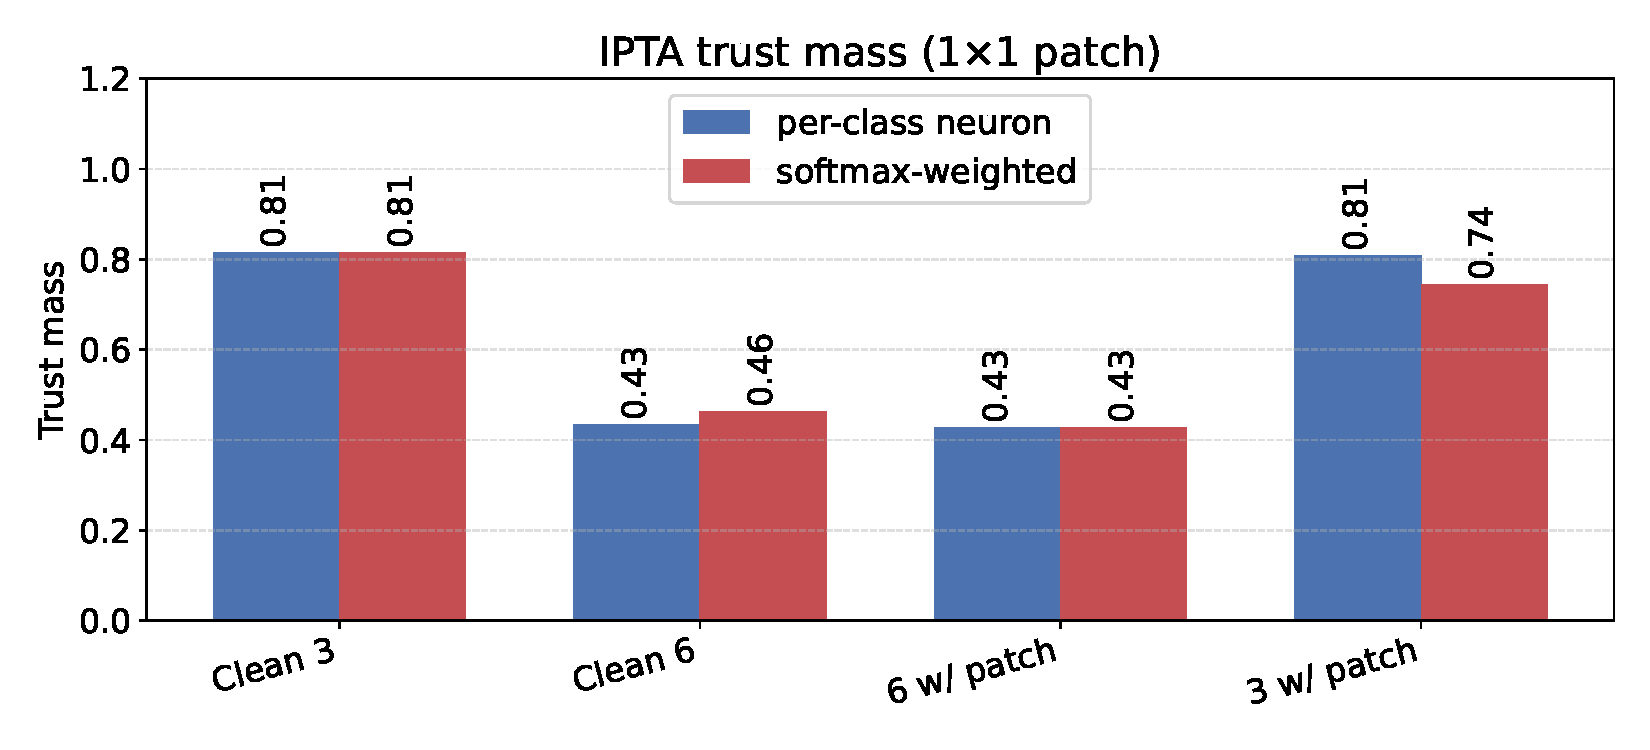
\includegraphics[width=0.3\textwidth]{latex/NN_Train_mnist_128_trust_trust_PathSize_1__ipta_trust_2a_vs_2c.pdf}%
}
\subfloat[{mnist\_128\_trust\_trust, ps=10}]{%
  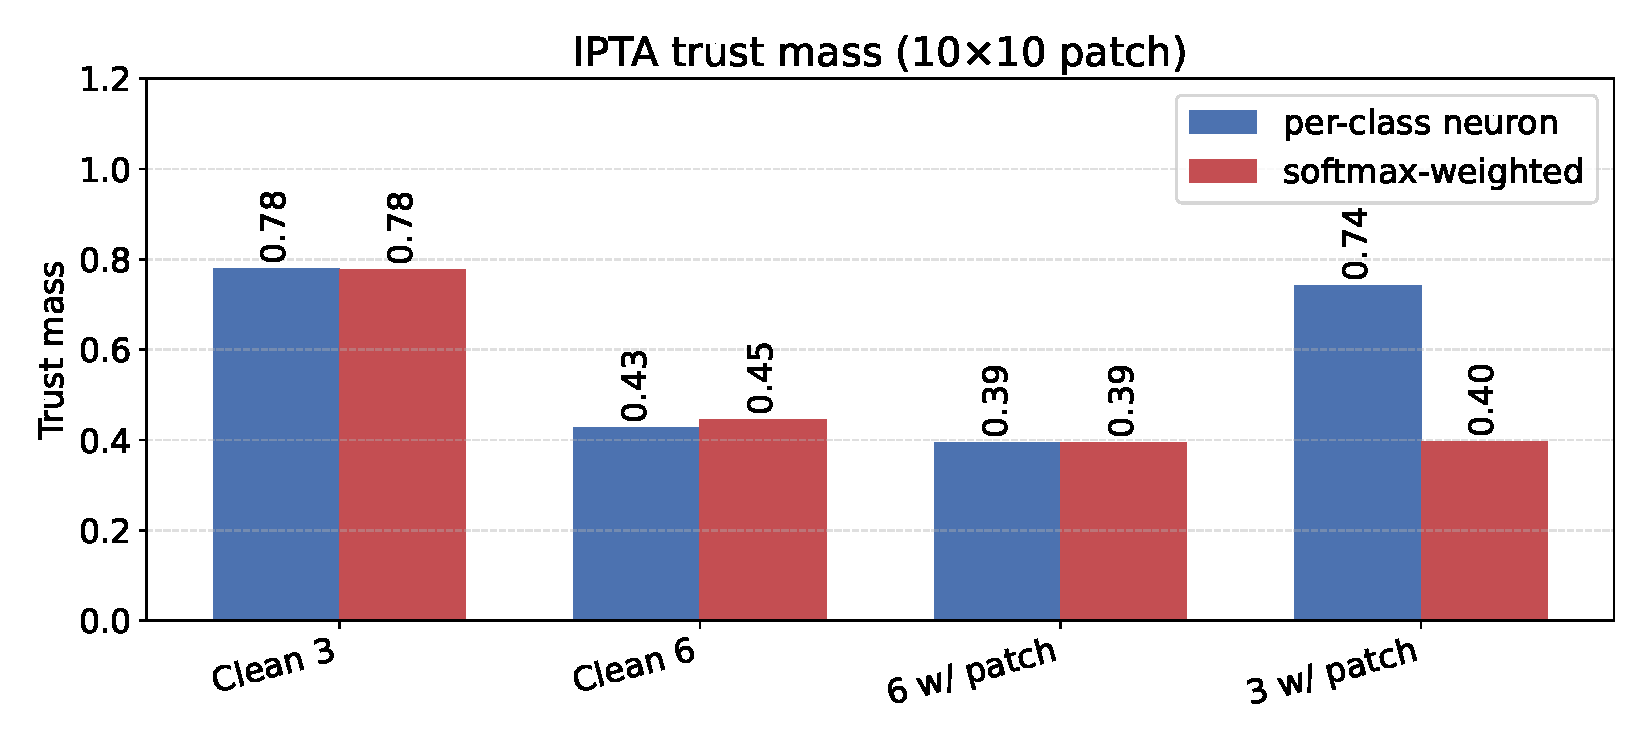
\includegraphics[width=0.3\textwidth]{latex/NN_Train_mnist_128_trust_trust_PathSize_10__ipta_trust_2a_vs_2c.pdf}%
}
\subfloat[{mnist\_128\_trust\_trust, ps=27}]{%
  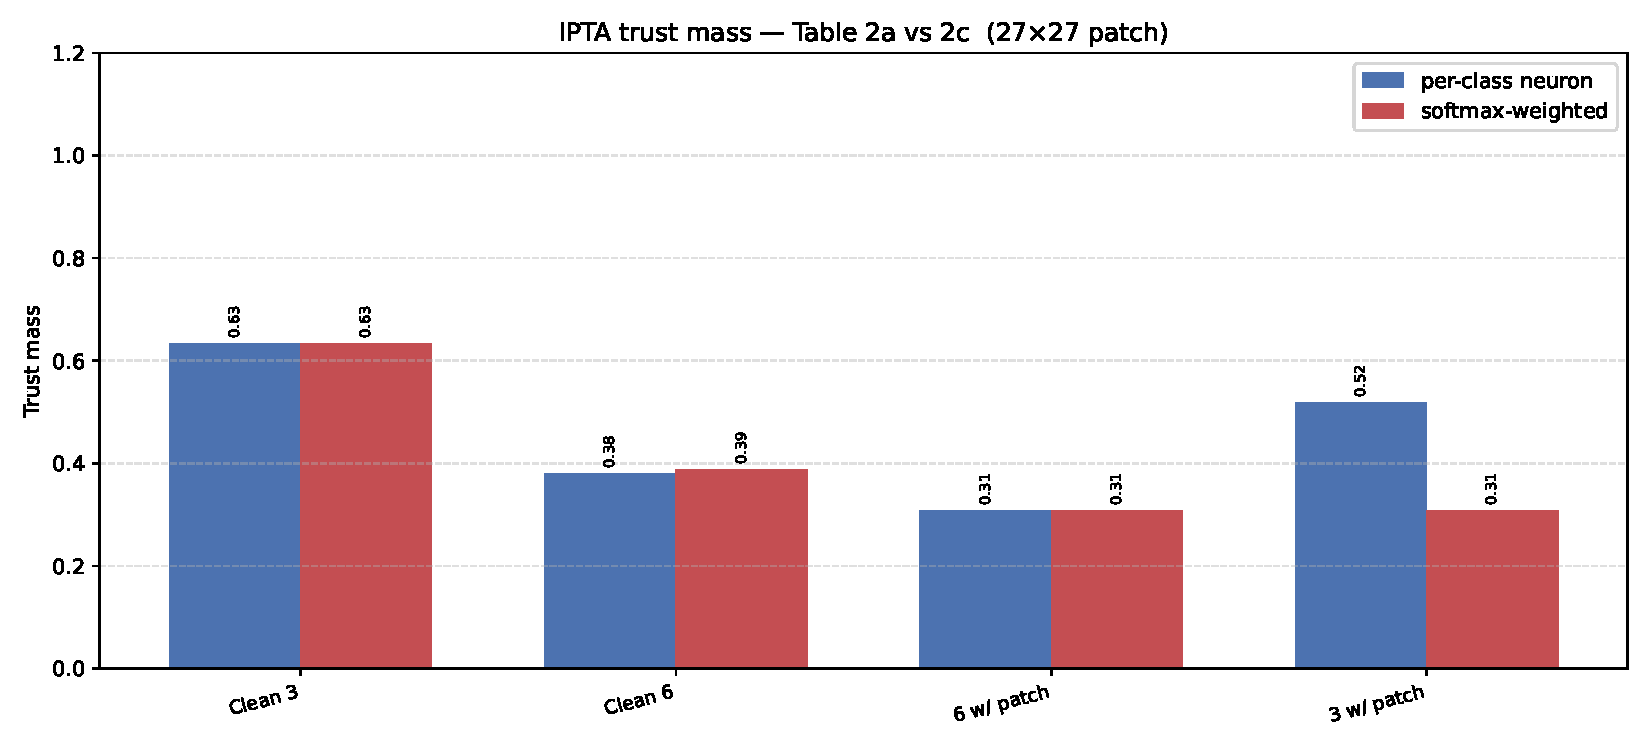
\includegraphics[width=0.3\textwidth]{latex/NN_Train_mnist_128_trust_trust_PathSize_27__ipta_trust_2a_vs_2c.pdf}%
}
\\
\subfloat[{mnist\_128\_trust\_trust, ps=4}]{%
  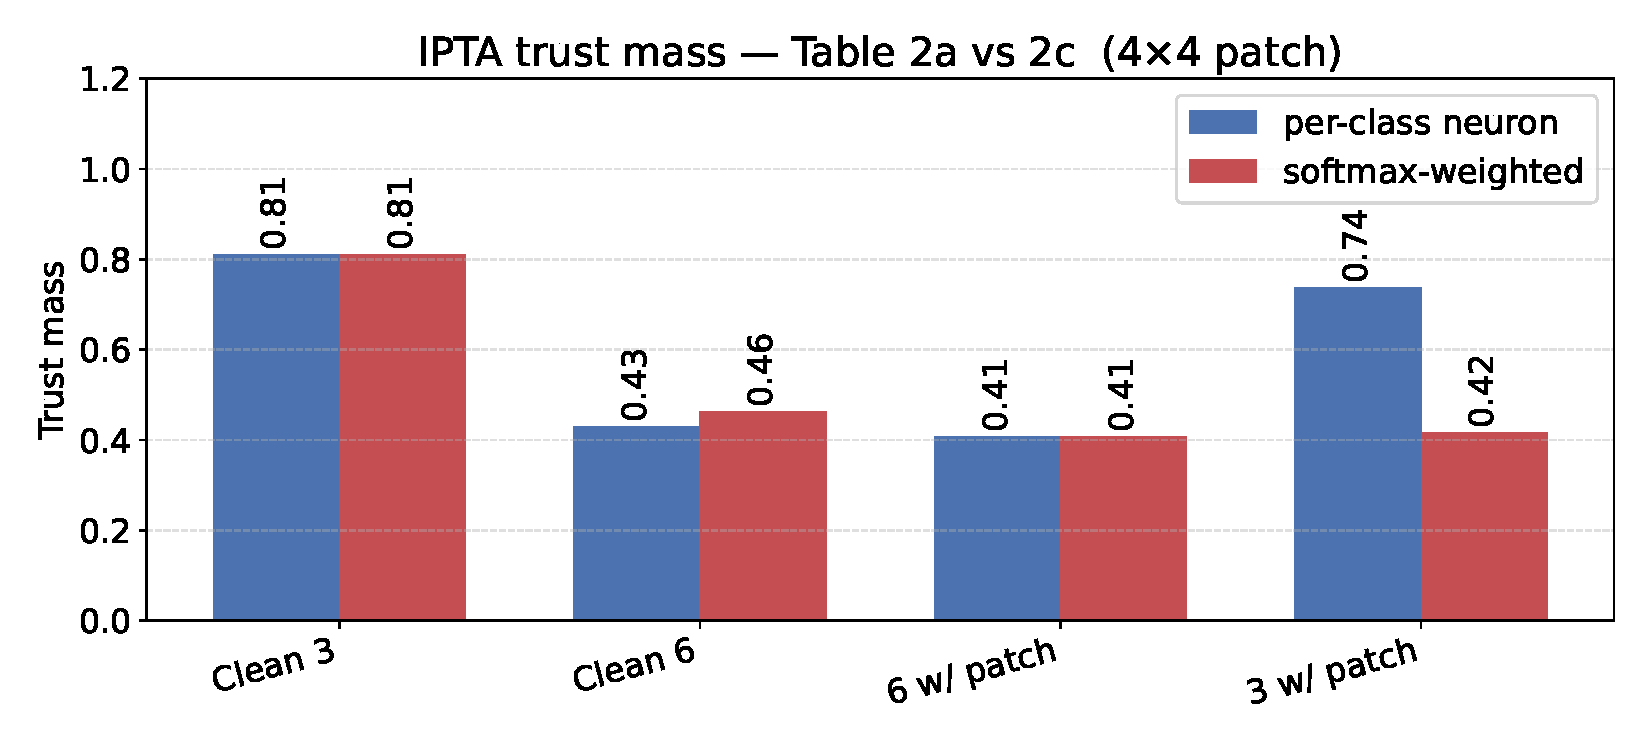
\includegraphics[width=0.3\textwidth]{latex/NN_Train_mnist_128_trust_trust_PathSize_4__ipta_trust_2a_vs_2c.pdf}%
}
\caption{IPTA -- Trust 2a vs 2c}
\end{figure}
